%% LyX 2.3.3 created this file.  For more info, see http://www.lyx.org/.
%% Do not edit unless you really know what you are doing.
\documentclass[12pt,english]{article}
\usepackage[osf]{mathpazo}
\renewcommand{\sfdefault}{lmss}
\renewcommand{\ttdefault}{lmtt}
\usepackage[T1]{fontenc}
\usepackage[latin9]{inputenc}
\usepackage[paperwidth=30cm,paperheight=35cm]{geometry}
\geometry{verbose,tmargin=3cm,bmargin=3cm}
\setlength{\parindent}{0bp}
\usepackage{mathrsfs}
\usepackage{amsmath}
\usepackage{amssymb}

\makeatletter
%%%%%%%%%%%%%%%%%%%%%%%%%%%%%% User specified LaTeX commands.
\usepackage{tikz}
\usetikzlibrary{matrix,arrows,decorations.pathmorphing}
\usetikzlibrary{shapes.geometric}
\usepackage{tikz-cd}
\usepackage{amsthm}
\usepackage{xparse,etoolbox}

\theoremstyle{plain}
\newtheorem{theorem}{Theorem}[section]
\newtheorem{lemma}[theorem]{Lemma}
\newtheorem{prop}{Proposition}[section]
\newtheorem{cor}{Corollary}
\theoremstyle{definition}
\newtheorem{defn}{Definition}[section]
\newtheorem{ex}{Exercise}
\newtheorem{sol}{Solution} 
\newtheorem{example}{Example}[section]
\theoremstyle{remark}
\newtheorem{rem}{Remark}
\newtheorem*{note}{Note}
\newtheorem{case}{Case}
\usepackage{graphicx}
\usepackage{amssymb}
\usepackage{tikz-cd}
\usetikzlibrary{calc,arrows,decorations.pathreplacing}
\tikzset{mydot/.style={circle,fill,inner sep=1.5pt},
commutative diagrams/.cd,
  arrow style=tikz,
  diagrams={>=latex},
}

\usepackage{babel}
\usepackage{hyperref}
\hypersetup{
    colorlinks,
    citecolor=blue,
    filecolor=blue,
    linkcolor=blue,
    urlcolor=blue
}
\usepackage{pgfplots}
\usetikzlibrary{decorations.markings}
\pgfplotsset{compat=1.9}


\newcommand{\blocktheorem}[1]{%
  \csletcs{old#1}{#1}% Store \begin
  \csletcs{endold#1}{end#1}% Store \end
  \RenewDocumentEnvironment{#1}{o}
    {\par\addvspace{1.5ex}
     \noindent\begin{minipage}{\textwidth}
     \IfNoValueTF{##1}
       {\csuse{old#1}}
       {\csuse{old#1}[##1]}}
    {\csuse{endold#1}
     \end{minipage}
     \par\addvspace{1.5ex}}
}

\raggedbottom

\blocktheorem{theorem}% Make theo into a block
\blocktheorem{defn}% Make defi into a block
\blocktheorem{lemma}% Make lem into a block
\blocktheorem{rem}% Make rem into a block
\blocktheorem{cor}% Make col into a block
\blocktheorem{prop}% Make prop into a block


\makeatletter
\newcommand*{\@old@slash}{}\let\@old@slash\slash
\def\slash{\relax\ifmmode\delimiter"502F30E\mathopen{}\else\@old@slash\fi}
\makeatother

\def\backslash{\delimiter"526E30F\mathopen{}}



\usepackage[bottom]{footmisc}

\makeatother

\usepackage{babel}
\begin{document}
\title{Measure Theory}

\maketitle
\tableofcontents{}

\newpage{}

\part{Class Notes}

\section{Introduction}

Measure theory is a central subject in analysis. Let us consider four
problems which helped lead to the development of measure theory.

\hfill

1) When we studied inner-products in Hilbert spaces, we considered
the inner-product space $(C[a,b],\langle\cdot,\cdot\rangle_{1})$,
where $C[a,b]$ is the $\mathbb{C}$-vector space of all continuous
functions defined on the interval $[a,b]$ and $\langle\cdot,\cdot\rangle_{1}$
is the inner-product defined by
\begin{equation}
\langle f,g\rangle=\int_{a}^{b}f(x)\overline{g(x)}\mathrm{d}x\label{eq:L1normbeg}
\end{equation}
for all $f,g\in C[a,b]$. One of the problems that we ran into when
studying this inner-product space is that it is \emph{not }a Hilbert
space. In other words, $C[a,b]$ is not complete with respect to topology
induced by this inner-product. It turns out however that just as how
$\mathbb{R}$ can be viewed as the ``completion'' of $\mathbb{Q}$
with respect to the usual topology on $\mathbb{Q}$ induced by the
usual absolute value $|\cdot|$, there is a similar space which can
be viewed as the ``completion'' of $C[a,b]$ with respect to the
topology induced by the inner-product $\langle\cdot,\cdot\rangle_{1}$.
Measure theory will give us a nice interpretation of what this completed
space looks like. 

\hfill

2) Now consider the normed linear space $(C[a,b],\|\cdot\|_{\infty})$,
where $\|\cdot\|_{\infty}$ is the supremum norm. This time $C[a,b]$
\emph{is} complete with respect to the topology induced by this norm.
In other words, $(C[a,b],\|\cdot\|_{\infty})$ is a Banach space.
In this case, we'd like to know what the dual space looks like. Recall
that the dual of a normed linear space $(\mathcal{X},\|\cdot\|)$
is defined to be the space $(\mathcal{X}^{*},\|\cdot\|)$ where
\[
\mathcal{X}^{*}:=\{\ell\colon\mathcal{X}\to\mathbb{C}\mid\ell\text{ is a bounded linear functional}\}
\]
and where the norm, denoted $\|\cdot\|$ again, is defined by
\[
\|\ell\|=\sup\{|\ell(x)|\mid\|x\|\leq1\}
\]
for all $\ell\in\mathcal{X}^{*}$. For instance, here are three examples
of a bounded linear functionals on $C[a,b]$ (with respect to the
sup norm)
\begin{align*}
\ell_{1}(f) & =\int_{a}^{b}f(x)\mathrm{d}x\\
\ell_{2}(f) & =f(a)\\
\ell_{3}(f) & =f(a)+f(b).
\end{align*}
Here again we will find that measure theory will give us a natural
interpretation of what the dual space of $C[a,b]$ looks like. We
shall that see that, in a certain sense, the bounded linear functionals
on $C[a,b]$ will correspond to different ways you can integrate on
$[a,b]$.

\hfill

3) The third problem we consider goes as follows: let $T\colon\mathcal{H}\to\mathcal{H}$
be a bounded linear map from a Hilbert space to itself. If $T$ is
compact and self-adjoint, then the Spectral Theorem tells us that
there exists an orthonormal basis of eigenvectors $(e_{n})$ with
eigenvalues $(\lambda_{n})$ such that
\[
Tx=\sum_{n=1}^{\infty}\lambda_{n}\langle x,e_{n}\rangle e_{n}
\]
for all $x\in\mathcal{H}$. Can we still get a spectral theorem if
we remove the compactness condition? It turns out that there is a
way to do this. We may not be able to completely show this in this
class (perhaps in a functional analysis class), but we will make progress
using measure theory.

\hfill

4) The foundations of probability theory is based on measure theory.
We will better understand the connection between probability theory
and measure theory. 

\hfill

~~~Let's go back to $C[a,b]$ equipped with the inner-product $\langle\cdot,\cdot\rangle_{1}$
described above. As we said, the main problem with $(C[a,b],\langle\cdot,\cdot\rangle_{1})$
is that this space is not complete. Ideally, we would like to be able
to measure ``the length'' of any subset of $\mathbb{R}$ such that
\begin{enumerate}
\item the length of an interval $(c,d)$ is $d-c$,
\item if we translate a set, its length should stay the same,
\item if $(E_{n})$ is a sequence of pairwise disjoint subsets of $\mathbb{R}$
with lengths $\mu(E_{n})$, then the length of their union satisfy
\[
\mu\left(\bigcup_{n=1}^{\infty}E_{n}\right)=\sum_{n=1}^{\infty}\mu(E_{n}).
\]
\end{enumerate}

\section{Intervals, Algebras, and Measures}

Throughout the rest of this section, we consider the normed linear
space $(C[a,b],\|\cdot\|)$\footnote{Unless otherwise specified, we will often simply write $C[a,b]$ instead
of $(C[a,b],\|\cdot\|)$ and view $C[a,b]$ as a normed linear space
equipped with the $L_{1}$ norm. } where, unless otherwise specified, $\|\cdot\|$ is the $L_{1}$ norm:
\[
\|f\|:=\int_{a}^{b}|f(x)|\mathrm{d}x
\]
for all $f\in C[a,b]$ where the integral is understood to be the
Riemann integral. It is easy to prove that $C[a,b]$ equipped with
the $L_{1}$ norm is a normed linear space, but it is not complete.
As shown in the Appendix, we know that we can construct the completion
of $C[a,b]$ using Cauchy sequences, but this space is a little too
abstract for our desires. We would like to describe the completion
of $C[a,b]$ in a more concrete way. More specifically, we'd like
to realize the completion of $C[a,b]$ as a quotient of a certain
space of functions (rather than as a quotient of a space of Cauchy
sequences). 

~~~Indeed, if $\mathcal{Y}$ is a dense subspace of a normed linear
space $\mathcal{X}$, then every bounded linear functional $\ell\colon\mathcal{Y}\to\mathbb{C}$
can be extended in a unique way to a bounded linear functional $\widetilde{\ell}\colon\mathcal{X}\to\mathbb{C}$
with the same norm. That is, $\widetilde{\ell}|_{\mathcal{Y}}=\ell$
and $\|\widetilde{\ell}\|=\|\ell\|$. The linear functional $\ell\colon C[a,b]\to\mathbb{C}$
defined by
\[
\ell(f)=\int_{a}^{b}f(x)\mathrm{d}x
\]
for all $f\in C[a.b]$ is bounded with $\|\ell\|=1$. So if we can
define the completion of $C[a,b]$ as a quotient of a space of functions,
then we will be able to compute $\widetilde{\ell}(f)$ for every $f$.
In turn, this can be naturally viewed as computing $\int_{a}^{b}f(x)\mathrm{d}x$.
This new integral will be called the \textbf{Lebesgue integral }and
the representative functions in this space will be called \textbf{Lebesgue
measurable functions}. Let us denote the completion of $C[a,b]$ with
respect to $\|\cdot\|$ by $(\mathscr{C}[a,b],\|\cdot\|)$, or more
simply $\mathscr{C}[a,b]$. 

\subsection{Intervals}

Unless otherwise specified, by a a \textbf{subinterval} \textbf{of
$[a,b]$}, we shall mean a subinterval of $[a,b]$ of the following
types: $(c,d)$, $(c,b]$, $[c,b)$, and $[c,d]$, where 
\[
-\infty<a\leq c\leq d\leq b<\infty.
\]
Note that $(c,c)=\emptyset$ and $[c,c]=\{c\}$ are considered intervals
as well. If $I$ is a subinterval of $[a,b]$, then the \textbf{indicator
function} $1_{I}\colon[a,b]\to\{0,1\}$ with respect to $I$ is defined
by
\[
1_{I}(x)=\begin{cases}
1 & \text{if }x\in I\\
0 & \text{if }x\notin I
\end{cases}
\]
for all $x\in[a,b]$. If $I$ is a subinterval of $[a,b]$, then it
closure in $[a,b]$ has the form
\[
\overline{I}=[c,d]
\]
for some $a\leq c\leq d\leq b$. In this case, we define the \textbf{length
}of $I$ to be
\[
\mathrm{length}(I)=d-c.
\]

We denote by $\mathcal{I}_{[a,b]}$ (or more simply just $\mathcal{I}$
if context is clear) to be the collection of all finite unions of
subintervals of $[a,b]$. 

\subsubsection{Collection of all Subintervals of $[a,b]$ Forms a Semialgebra of
Sets}

\begin{defn}\label{defn} A nonempty collection $\mathcal{E}$ of
subsets of $X$ is said to be a \textbf{semialgebra }of sets if it
satisfies the following properties:
\begin{enumerate}
\item $\emptyset\in\mathcal{E}$;
\item If $E,F\in\mathcal{E}$, then $E\cap F\in\mathcal{E}$;
\item If $E\in\mathcal{E}$, then $E^{c}$ is a finite disjoint union of
sets from $\mathcal{E}$. 
\end{enumerate}
\end{defn}

\begin{prop}\label{prop} The collection of all subintervals of $[a,b]$
forms a semialgebra of sets. \end{prop}

\begin{proof} Let $\mathcal{I}$ denote the collection of all subintervals
of $[a,b]$. We have $\emptyset\in\mathcal{I}$ since $\emptyset=(c,c)$
for any $c\in[a,b]$. Now we show $\mathcal{I}$ is closed under finite
intersections. Let $I_{1}$ and $I_{2}$ be subintervals of $[a,b]$.
Taking the closure of $I_{1}$ and $I_{2}$ gives us closed intervals,
say
\[
\overline{I}_{1}=[c_{1},d_{1}]\quad\text{and}\quad\overline{I}_{2}=[c_{2},d_{2}].
\]

Assume without loss of generality that $c_{1}\leq c_{2}$. If $d_{1}<c_{2}$,
then $I_{1}\cap I_{2}=\emptyset$, so assume that $d_{1}\geq c_{2}$.
If $d_{1}\geq d_{2}$, then $I_{1}\cap I_{2}=I_{2}$, so assume that
$d_{1}<d_{2}$. If $c_{1}=c_{2}$, then $I_{1}\cap I_{2}=I_{1}$,
so assume that $c_{2}>c_{1}$. So we have reduced the case to where
\[
c_{1}<c_{2}\leq d_{1}<d_{2}.
\]

With these assumptions in mind, we now consider four cases:

\hfill

\textbf{Case 1: }If\textbf{ $I_{1}=[c_{1},d_{1}]$ }or $I_{1}=(c_{1},d_{1}]$\textbf{
}and $I_{2}=[c_{2},d_{2}]$ or $I_{2}=[c_{2},d_{2})$, then $I_{1}\cap I_{2}=[c_{2},d_{1}]$.

\hfill

\textbf{Case 2: }If\textbf{ $I_{1}=[c_{1},d_{1})$ }or $I_{1}=(c_{1},d_{1})$\textbf{
}and $I_{2}=[c_{2},d_{2}]$ or $I_{2}=[c_{2},d_{2})$, then $I_{1}\cap I_{2}=[c_{2},d_{1})$.

\hfill

\textbf{Case 3: }If\textbf{ $I_{1}=[c_{1},d_{1}]$ }or $I_{1}=(c_{1},d_{1})$\textbf{
}and $I_{2}=(c_{2},d_{2}]$ or $I_{2}=(c_{2},d_{2})$, then $I_{1}\cap I_{2}=(c_{2},d_{1})$.

\hfill

\textbf{Case 4: }If\textbf{ $I_{1}=[c_{1},d_{1})$ }or $I_{1}=(c_{1},d_{1})$\textbf{
}and $I_{2}=(c_{2},d_{2}]$ or $I_{2}=(c_{2},d_{2})$, then $I_{1}\cap I_{2}=(c_{2},d_{1})$.

\hfill

In all cases, we see that $I_{1}\cap I_{2}$ is a subinterval of $[a,b]$. 

~~~Now we show that compliments can be expressed as finite disjoint
unions. Let $I$ be a subinterval of $[a,b]$ and write $\overline{I}=[c,d]$.
We consider four cases:

\hfill

\textbf{Case 1: }If $I=[c,d]$, then $I^{c}=[a,c)\cup(d,b]$.

\hfill

\textbf{Case 2: }If $I=(c,d]$, then $I^{c}=[a,c]\cup(d,b]$.

\hfill

\textbf{Case 3: }If $I=[c,d)$, then $I^{c}=[a,c)\cup[d,b]$.

\hfill

\textbf{Case 4: }If $I=(c,d)$, then $I^{c}=[a,c]\cup[d,b]$.

\hfill

Thus in all cases, we can express $I^{c}$ as a disjoint union of
intervals since $a\leq c\leq d\leq b$. \end{proof}

\subsubsection{Indicator Function $1_{I}$ Represents an Element in $\mathscr{C}[a,b]$}

The next proposition tells us that $1_{I}$ should represent an element
in $\mathscr{C}[a,b]$ for all subintervals $I$ of $[a,b]$ and that
$\|1_{I}\|=\mathrm{length}(I)$. 

\begin{prop}\label{prop} Let $I$ be a subinterval of $[a,b]$. Then
there exists a Cauchy sequence $(f_{n})$ in $(C[a,b],\|\cdot\|)$
such that $(f_{n})$ converges pointwise to $1_{I}$ on $[a,b]$.
Moreover we have
\[
\lim_{n\to\infty}\|f_{n}\|=\mathrm{length}(I).
\]
\end{prop}

\begin{proof} If $I=\emptyset$, then we take $f_{n}=0$ for all
$n\in\mathbb{N}$. Thus assume $I$ is a nonempty subinterval of $[a,b]$.
We consider two cases; namely $I=(c,d)$ and $I=[c,d]$. The other
cases ($I=(c,d]$ and $I=[c,d)$) will easily be seen to be a mixture
of these two cases.

\hfill

\textbf{Case 1}: Suppose $I=[c,d]$. For each $n\in\mathbb{N}$, define

\[
f_{n}(x)=\begin{cases}
0 & \text{if }a\leq x<c-\left(\frac{c-a}{n}\right)\\
\frac{n}{c-a}(x-c)+1 & \text{if }c-\left(\frac{c-a}{n}\right)\leq x<c\\
1 & \text{if }c\leq x\leq d\\
\frac{n}{d-b}(x-d)+1 & \text{if }d<x\leq d+\left(\frac{b-d}{n}\right)\\
0 & \text{if }d+\left(\frac{b-d}{n}\right)<x\leq b
\end{cases}
\]

The image below gives the graphs for $f_{1}$, $f_{2}$, and $f_{3}$
in the case where $[a,b]=[0,3]$ and $[c,d]=[1,2]$. 

\begin{center}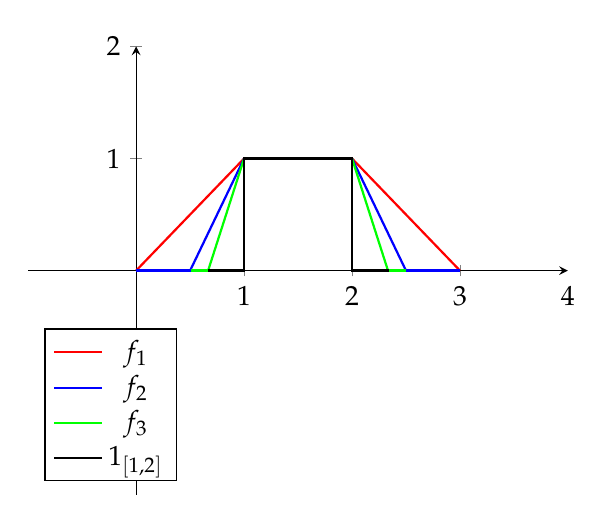
\begin{tikzpicture}\begin{axis}[axis lines = middle, 
xmin=-1,xmax=4,
ymin=-2,ymax=2,     
xtick={0,1,2,3,4},     
ytick={1,2},
legend pos= south west,]


\addplot [domain=0:1,samples=100,color=red,thick] ({x}, {x});
\addplot [domain=0:0.5,samples=100,color=blue,thick] ({x}, {0});
\addplot [domain=0.51:0.666,samples=100,color=green,thick] ({x}, {0});
\addplot [domain=0.666:1,samples=100,color=black,thick] ({x}, {0});


\addplot [domain=1:2,samples=100,color=red,thick] ({x}, {1});
\addplot [domain=2:3,samples=100,color=red,thick] ({x}, {-x + 3});

\addplot [domain=0:0.5,samples=100,color=blue,thick] ({x}, {0});
\addplot [domain=0.5:1,samples=100,color=blue,thick] ({x}, {2*x - 1});
\addplot [domain=1:2,samples=100,color=blue,thick] ({x}, {1});
\addplot [domain=2:2.5,samples=100,color=blue,thick] ({x}, {-2*x + 5});
\addplot [domain=2.5:3,samples=100,color=blue,thick] ({x}, {0});

\addplot [domain=0.51:0.666,samples=100,color=green,thick] ({x}, {0});
\addplot [domain=0.666:1,samples=100,color=green,thick] ({x}, {3*x - 2});
\addplot [domain=1:2,samples=100,color=green,thick] ({x}, {1});
\addplot [domain=2:2.333,samples=100,color=green,thick] ({x}, {-3*x + 7});
\addplot [domain=2.333:2.49,samples=100,color=green,thick] ({x}, {0});

\addplot [domain=0.666:1,samples=100,color=black,thick] ({x}, {0});
\addplot [domain=1:2,samples=100,color=black,thick] ({x}, {1});
\addplot [domain=2:2.333,samples=100,color=black,thick] ({x}, {0});


\node[] (x) at (axis cs:1,-0.1) {$$};
\node[] (y) at (axis cs:1,1.1) {$$};
\node[] (z) at (axis cs:2,-0.1) {$$};
\node[] (w) at (axis cs:2,1.1) {$$};

\draw [color=black,thick] (x) -- (y);
\draw [color=black,thick] (z) -- (w);



\addlegendentry{$ f_1 $} 
\addlegendentry{$ f_2 $}
\addlegendentry{$ f_3 $} 
\addlegendentry{$ 1_{[1,2] }$} 

\end{axis}\end{tikzpicture}\end{center}

For each $n\in\mathbb{N}$, the function $f_{n}$ is continuous since
each of its segments is continuous and are equal on their boundaries.

~~~Let us check that $(f_{n})$ converges pointwise to $1_{I}$:
If $x\in[a,c)$, then we choose $N\in\mathbb{N}$ such that 
\[
x\leq c-\left(\frac{c-a}{N}\right).
\]
Then $f_{n}(x)=0$ for all $n\geq N$. Thus
\[
\lim_{n\to\infty}f_{n}(x)=0=1_{I}(x).
\]

Similarly, if $x\in(d,b]$, then we choose $N\in\mathbb{N}$ such
that
\[
x\geq d+\left(\frac{b-d}{N}\right).
\]
Then $f_{n}(x)=0$ for all $n\geq N$. Thus
\[
\lim_{n\to\infty}f_{n}(x)=0=1_{I}(x).
\]

Finally, if $x\in[c,d]$, then $f_{n}(x)=1$ for all $n\in\mathbb{N}$
by definition and thus
\[
\lim_{n\to\infty}f_{n}(x)=0=1_{I}(x).
\]

~~~Let us check that $(f_{n})$ is Cauchy in $(C[a,b],\|\cdot\|_{1})$.
Let $\varepsilon>0$. Choose $N\in\mathbb{N}$ such that 
\[
\frac{c-a+b-d}{n}<\varepsilon
\]
for all $n\geq N$. Then $n\geq m\geq N$ implies
\begin{align*}
\|f_{n}-f_{m}\|_{1} & =\int_{a}^{b}|f_{n}(x)-f_{m}(x)|\mathrm{d}x\\
 & =\int_{a}^{b}(f_{n}(x)-f_{m}(x))\mathrm{d}x\\
 & =\int_{c-\left(\frac{c-a}{m}\right)}^{c}(f_{n}(x)-f_{m}(x))\mathrm{d}x+\int_{d}^{d+\left(\frac{b-d}{m}\right)}(f_{n}(x)-f_{m}(x))\mathrm{d}x\\
 & \leq\int_{c-\left(\frac{c-a}{m}\right)}^{c}\mathrm{d}x+\int_{d}^{d+\left(\frac{b-d}{m}\right)}\mathrm{d}x\\
 & =\frac{c-a}{m}+\frac{b-d}{m}\\
 & =\frac{c-a+b-d}{m}\\
 & <\varepsilon.
\end{align*}
Thus the sequence $(f_{n})$ is Cauchy in $(C[a,b],\|\cdot\|_{1})$. 

~~~Finally, we check that $\|f_{n}\|_{1}\to\mathrm{length}(I)$
as $n\to\infty$. We have
\begin{align*}
d-c & \leq\|f_{n}\|_{1}\\
 & =\int_{a}^{b}|f_{n}(x)|\mathrm{d}x\\
 & =\int_{a}^{b}f_{n}(x)\mathrm{d}x\\
 & =\int_{c-\left(\frac{c-a}{n}\right)}^{c}f_{n}(x)\mathrm{d}x+\int_{c}^{d}\mathrm{d}x+\int_{d}^{d+\left(\frac{b-d}{n}\right)}f_{n}(x)\mathrm{d}x\\
 & \leq\int_{c-\left(\frac{c-a}{n}\right)}^{c}\mathrm{d}x+\int_{c}^{d}\mathrm{d}x+\int_{d}^{d+\left(\frac{b-d}{n}\right)}\mathrm{d}x\\
 & =\frac{c-a}{n}+d-c+\frac{b-d}{n}\\
 & \to d-c.
\end{align*}
Thus for each $n\in\mathbb{N}$, we have 
\begin{equation}
d-c\leq\|f_{n}\|_{1}\leq d-c+\frac{c-a+b-d}{n}.\label{eq:ineqca}
\end{equation}
By taking $n\to\infty$ in (\ref{eq:ineqca}), we see that
\begin{align*}
\lim_{n\to\infty}\|f_{n}\|_{1} & =d-c\\
 & =\mathrm{length}(I).
\end{align*}

\hfill

\textbf{Case 2}: Suppose $I=(c,d)$. For each $n\geq2$, define

\[
f_{n}(x)=\begin{cases}
0 & \text{if }a\leq x\leq c\\
\frac{n}{d-c}(x-c) & \text{if }c<x\leq c+\left(\frac{d-c}{n}\right)\\
1 & \text{if }c+\left(\frac{d-c}{n}\right)\leq x\leq d-\left(\frac{d-c}{n}\right)\\
\frac{n}{c-d}(x-d) & \text{if }d-\left(\frac{d-c}{n}\right)\leq x\leq d\\
0 & \text{if }d\leq x\leq b
\end{cases}
\]

The image below gives the graphs for $f_{2}$, $f_{3}$, and $f_{4}$
in the case where $[a,b]=[0,3]$ and $(c,d)=(1,2)$. 

\begin{center}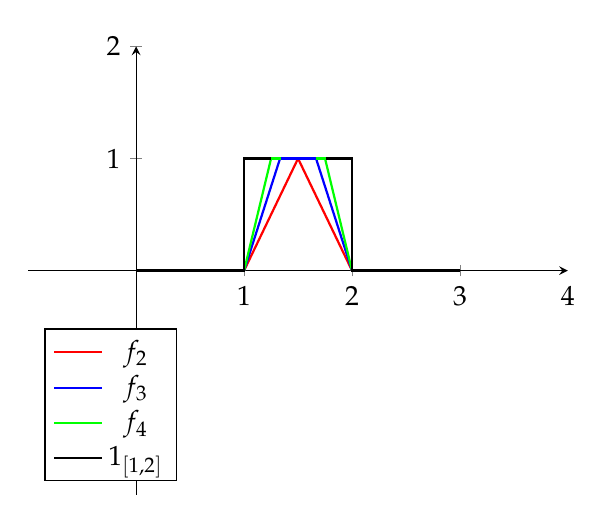
\begin{tikzpicture}\begin{axis}[axis lines = middle, 
xmin=-1,xmax=4,
ymin=-2,ymax=2,     
xtick={0,1,2,3,4},     
ytick={1,2},
legend pos= south west,]



\addplot [domain=0:1,samples=100,color=red,thick] ({x}, {0});
\addplot [domain=0:1,samples=100,color=blue,thick] ({x}, {0});
\addplot [domain=0:1,samples=100,color=green,thick] ({x}, {0});
\addplot [domain=0:1,samples=100,color=black,thick] ({x}, {0});





\addplot [domain=1:1.5,samples=100,color=red,thick] ({x}, {2*x - 2});
\addplot [domain=1.5:2,samples=100,color=red,thick] ({x}, {-2*x +4 });
\addplot [domain=2:3,samples=100,color=red,thick] ({x}, {0});

\addplot [domain=1:1.333,samples=100,color=blue,thick] ({x}, {3*x - 3});
\addplot [domain=1.333:1.666,samples=100,color=blue,thick] ({x}, {1});
\addplot [domain=1.666:2,samples=100,color=blue,thick] ({x}, {-3*x +6 });
\addplot [domain=2:3,samples=100,color=blue,thick] ({x}, {0});

\addplot [domain=1:1.25,samples=100,color=green,thick] ({x}, {4*x - 4});
\addplot [domain=1.25:1.333,samples=100,color=green,thick] ({x}, {1});
\addplot [domain=1.666:1.75,samples=100,color=green,thick] ({x}, {1});
\addplot [domain=1.75:2,samples=100,color=green,thick] ({x}, {-4*x +8 });
\addplot [domain=2:3,samples=100,color=green,thick] ({x}, {0});

\addplot [domain=1:1.24,samples=100,color=black,thick] ({x}, {1});
\addplot [domain=1.76:2,samples=100,color=black,thick] ({x}, {1});
\addplot [domain=2:3,samples=100,color=black,thick] ({x}, {0});


\node[] (x) at (axis cs:1,-0.1) {$$};
\node[] (y) at (axis cs:1,1.1) {$$};
\node[] (z) at (axis cs:2,-0.1) {$$};
\node[] (w) at (axis cs:2,1.1) {$$};

\draw [color=black,thick] (x) -- (y);
\draw [color=black,thick] (z) -- (w);


\addlegendentry{$ f_2 $} 
\addlegendentry{$ f_3 $}
\addlegendentry{$ f_4 $} 
\addlegendentry{$ 1_{[1,2] }$} 



\end{axis}\end{tikzpicture}\end{center}

That $(f_{n})$ is a Cauchy sequence of continuous funtions in $(C[a,b],\|\cdot\|_{1})$
which converges pointwise to $1_{I}$ and $\|f_{n}\|_{1}\to\mathrm{length}(I)$
as $n\to\infty$ follows from similar arguments used in case 1. \end{proof} 

\begin{rem}\label{rem} Note that $1_{[c,c]}$ is not the zero function,
even though $\|1_{[c,c]}\|=0$. Thus we need to identify the function
$1_{[c,c]}$ and the constant zero function in $\mathscr{C}[a,b]$.
In other words, $1_{[c,c]}$ and the constant zero function should
represent the same element in $\mathscr{C}[a,b]$. Similarly, we have
\begin{align*}
\|1_{(c,d]}-1_{(c,d)}\| & =\|1_{[d,d]}\|\\
 & =0,
\end{align*}
and so the functions $1_{(c,d]}$ and $1_{(c,d)}$ should represent
the same element in $\mathscr{C}[a,b]$. \end{rem}

\subsubsection{Finite Sums of Indicator Functions of Intervals Represents Elements
in $\mathscr{C}[a,b]$}

Let $E$ be any finite union of intervals. Since the collection of
all intervals forms a semialgebra, we can express $E$ as a finite
union of disjoint intervals, say
\[
E=\bigcup_{i=1}^{k}I_{i}
\]
where $I_{i}\cap I_{j}=\emptyset$ whenever $i\neq j$. The next proposition
tells us that $1_{E}$ should represent an element in $\mathscr{C}[a,b]$
and that 
\[
\|1_{E}\|=\sum_{i=1}^{k}\mathrm{length}(I_{i})
\]
. 

\begin{prop}\label{prop} With the notation as above, there exists
a Cauchy sequence $(f_{n})$ in $(C[a,b],\|\cdot\|)$ such that $(f_{n})$
converges pointwise to $1_{E}$ on $[a,b]$. Moreover we have
\begin{equation}
\lim_{n\to\infty}\|f_{n}\|=\sum_{i=1}^{k}\mathrm{length}(I_{i}).\label{eq:sumcauchydisjoint}
\end{equation}

\end{prop}

\begin{proof} For each $1\leq i\leq k$, choose a Cauchy sequence
$(f_{n}^{i})_{n\in\mathbb{N}}$ such that $(f_{n}^{i})$ converges
pointwise to $1_{I_{i}}$ on $[a,b]$ and satisfies 
\[
\lim_{n\to\infty}\|f_{n}^{i}\|=\mathrm{length}(I_{i}).
\]
For each $n\in\mathbb{N}$, set $f_{n}=\sum_{i=1}^{k}f_{n}^{i}$.
We claim that $(f_{n})$ is a Cauchy sequence that converges pointwise
to $1_{E}$ and satisfies (\ref{eq:sumcauchydisjoint}). Indeed, it
is Cauchy since a sum of Cauchy sequences is Cauchy. Let us check
that it converges pointwise to $1_{E}$. Let $x\in E$ and let $\varepsilon>0$.
Then $x\in I_{i}$ for some $1\leq i\leq k$, and so there exists
an $N\in\mathbb{N}$ such that $n\geq N$ implies
\[
|f_{n}^{i}(x)-1_{I^{i}}(x)|<\frac{\varepsilon}{k}
\]
for all $1\leq i\leq n$. Choose such an $N\in\mathbb{N}$. Then $n\geq N$
implies
\begin{align*}
|f_{n}(x)-1_{E}(x)| & =\left|\sum_{i=1}^{k}f_{n}^{i}(x)-\sum_{i=1}^{k}1_{I_{i}}(x)\right|\\
 & \leq\sum_{i=1}^{k}|f_{n}^{i}(x)-1_{I_{i}}(x)|\\
 & <\sum_{i=1}^{k}\frac{\varepsilon}{k}\\
 & =\varepsilon.
\end{align*}
It follows that $f_{n}$ converges pointwise to $1_{E}$. Finally,
let us check that (\ref{eq:sumcauchydisjoint}) holds. Let $\varepsilon>0$.
Without loss of generality, we may assume that $\|f_{n}^{i}\|\geq\mathrm{length}(I_{i})$
and $\|f_{n}\|\geq\mathrm{length}(E)$ for all $1\leq i\leq k$ and
for all $n\in\mathbb{N}$. Choose $N\in\mathbb{N}$ such that $n\geq N$
implies
\[
\|f_{n}^{i}\|-\mathrm{length}(I_{i})<\frac{\varepsilon}{k}
\]
for all $i=1,\dots,k$. Then $n\geq N$ implies
\begin{align*}
\|f_{n}\|-\mathrm{length}(E) & =\left\Vert \sum_{i=1}^{k}f_{n}^{i}\right\Vert -\mathrm{length}\left(\bigcup_{i=1}^{k}I_{i}\right)\\
 & =\left\Vert \sum_{i=1}^{k}f_{n}^{i}\right\Vert -\sum_{i=1}^{k}\mathrm{length}(I_{i})\\
 & \leq\sum_{i=1}^{k}\|f_{n}^{i}\|-\sum_{i=1}^{k}\mathrm{length}(I_{i})\\
 & <\varepsilon.
\end{align*}
It follows that (\ref{eq:sumcauchydisjoint}) holds. \end{proof}

\subsubsection{Well-Definedness of Length}

Given the result above, it seems logical that the indiciator function
of any set $E$ which can be expressed as a finite disjoint union
of intervals should represent an element in $\mathscr{C}[a,b]$. Moreover,
the norm of $1_{E}$ (or the measure of $E$) ought to be the sums
of the norms of $1_{I_{i}}$ (or the sum of the lengths of $I_{i}$).
We need to be careful though! We may have two different ways of expressing
$E$ as a finite disjoint union, say
\[
E=\bigcup_{i=1}^{k}I_{i}\quad\text{and}\quad E=\bigcup_{i'=1}^{k'}I'_{i'}.
\]
We must check that if this is the case, then
\[
\sum_{i=1}^{k}\mathrm{length}(I_{i})=\sum_{i'=1}^{k'}\mathrm{length}(I'_{i'}).
\]
It turns out that this is indeed true, but we will leave the proof
of this to the reader.

\subsection{Algebras}

\begin{defn} Let $\mathcal{A}$ be a nonempty collection of subsets
of $X$. We make the following definitions. 
\begin{enumerate}
\item We say $\mathcal{A}$ is an \textbf{algebra }if it is closed under
finite intersections and is closed under complements. To be closed
under finite intersections means that if $A,B\in\mathcal{A}$, the
$A\cap B\in\mathcal{A}$. To be closed under complements means that
if $A\in\mathcal{A}$, then $A^{c}\in\mathcal{A}$. Note that in this
case, we automatically have $\emptyset\in\mathcal{A}$. Indeed, since
$\mathcal{A}$ is nonempty, we can choose $A\in\mathcal{A}$. Then
$\emptyset=A\cap A^{c}\in\mathcal{A}$. Note also that $\mathcal{A}$
is closed under finite unions. This means that if $A,B\in\mathcal{A}$,
then $A\cup B\in\mathcal{A}$. Indeed, we have
\begin{align*}
A\cup B & =((A\cup B)^{c})^{c}\\
 & =(A^{c}\cap B^{c})^{c}\\
 & \in\mathcal{A}.
\end{align*}
\item We say $\mathcal{A}$ is a \textbf{semialgebra }if it contains the
emptyset, is closed under finite intersections, and complements can
be expressed by finite disjoint unions of members of $\mathcal{A}$.
The last part means if $A\in\mathcal{A}$, then there exists a pairwise
disjoint sequence $A_{1},\dots,A_{n}\in\mathcal{A}$ such that $A^{c}=\bigcup_{i=1}^{n}A_{i}.$
Here we need include $\emptyset\in\mathcal{A}$ as part of the definition,
since we don't necessarily get this from the other two axioms. However
something that we do get from the other two aximos is that \emph{relative
}complements can be expressed by finite disjoint unions of members
of $\mathcal{A}$. Indeed, let $A,B\in\mathcal{A}$. Choose a pairwise
disjoint sequence $B_{1},\dots,B_{n}\in\mathcal{A}$ such that $B^{c}=\bigcup_{i=1}^{n}B_{i}$.
Then we have
\begin{align*}
A\backslash B & =A\cap B^{c}\\
 & =A\cap\left(\bigcup_{i=1}^{n}B_{i}\right)\\
 & =\bigcup_{i=1}^{n}A\cap B_{i},
\end{align*}
where $A\cap B_{1},\dots A\cap B_{n}$ is a pairwise disjoint sequence
of members of $\mathcal{A}$. Clearly every algebra is a semialgebra. 
\item We say $\mathcal{A}$ is a $\sigma$\textbf{-algebra }if it is closed
under \emph{countable }intersections and is closed under complements.
To be closed under countable intersections means that if $(A_{n})$
is a sequence of members of $\mathcal{A}$, the $\bigcup_{n=1}^{\infty}A_{n}\in\mathcal{A}$.
Clearly every $\sigma$-algebra is an algebra.
\end{enumerate}
\end{defn}

\begin{rem}\label{rem} We typically use $\mathcal{E}$ to denote
a semialgebra, $\mathcal{A}$ to denote an algebra, and $\mathcal{M}$
to denote a $\sigma$-algebra. \end{rem}

\subsubsection{Obtaining an Algebra from a Semialgebra}

\begin{prop}\label{prop} Let $\mathcal{E}$ be a semialgebra of subsets
of $X$. Then the collection $\mathcal{A}$ consisting of all sets
which are finite disjoint union of sets in $\mathcal{E}$ forms an
algebra of sets. \end{prop}

\begin{proof} Let us show that $\mathcal{A}$ is closed under finite
intersections. Let $A,A'\in\mathcal{A}$ and express $A$ and $A'$
as a finite disjoint union of members of $\mathcal{E}$, say
\[
A=E_{1}\cup\cdots\cup E_{n}\quad\text{and}\quad A'=E'_{1}\cup\cdots\cup E'_{n'}.
\]
Then we have
\begin{align*}
A\cap A' & =\left(\bigcup_{i=1}^{n}E_{i}\right)\cap\left(\bigcup_{i'=1}^{n'}E'_{i'}\right)\\
 & =\bigcup_{i'=1}^{n'}\left(\left(\bigcup_{i=1}^{n}E_{i}\right)\cap E'_{i'}\right)\\
 & =\bigcup_{i'=1}^{n'}\left(\bigcup_{i=1}^{n}E_{i}\cap E'_{i'}\right)\\
 & =\bigcup_{\substack{1\leq i\leq n\\
1\leq i'\leq n'
}
}E_{i}\cap E'_{i'}
\end{align*}
where the union is disjoint since the $E_{i}$ and $E'_{i'}$ are
disjoint from one another whenever $i\neq i'$. Thus $A\cap A'\in\mathcal{A}$,
and hence $\mathcal{A}$ is closed under finite intersections. 

~~~Now let us show that $\mathcal{A}$ is closed under complements.
Let $A\in\mathcal{A}$ and express $A$ as a finite disjoint union
of members of $\mathcal{E}$, say
\[
A=\bigcup_{i=1}^{n}E_{i}.
\]
For each $E_{i}$, express $E_{i}^{c}$ as a finite disjoint union
of members of $E$, say
\[
E_{i}^{c}=\bigcup_{j_{i}=1}^{n_{i}}E_{i,j_{i}}.
\]
Then we have
\begin{align*}
A^{c} & =\left(\bigcup_{i=1}^{n}E_{i}\right)^{c}\\
 & =\bigcap_{i=1}^{n}E_{i}^{c}\\
 & =\bigcap_{i=1}^{n}\bigcup_{j_{i}=1}^{n_{i}}E_{i,j_{i}}\\
 & =\bigcup_{j_{i}=1}^{n_{i}}\bigcap_{i=1}^{n}E_{i,j_{i}}
\end{align*}
where we were allowed to commute the union with the intersection from
the third line to the fourth line since these are finite unions and
finite intersections. Also, the union is disjoint since the $E_{i,j_{i}}$
and $E_{i,j_{i}'}$ are disjoint from one another whenever $j_{i}\neq j_{i}'$.
Thus $A^{c}\in\mathcal{A}$, and hence $\mathcal{A}$ is closed complements.
\end{proof}

\subsubsection{Ascendification, Contractifcation, and Disjointification}

Let $\mathcal{A}$ be an algebra of subsets of $X$ and let $(A_{n})$
be a sequence in $\mathcal{A}$. There are several operations we can
perform on $(A_{n})$ to obtain a new sequence in $\mathcal{A}$.
They are called \textbf{ascendification}, \textbf{contractification},
and \textbf{disjointification}.

\begin{defn}\label{defn} Let $\mathcal{A}$ be an algebra of subsets
of $X$ and let $(A_{n})$ be a sequence in $\mathcal{A}$.
\begin{enumerate}
\item Define the sequence $(B_{n})$ as follows: for all $n\in\mathbb{N}$,
we set $B_{n}=\bigcup_{i=1}^{n}A_{i}$. Since $\mathcal{A}$ is closed
under finite unions, it is clear that $(B_{n})$ is a sequence in
$\mathcal{A}$. The $(B_{n})$ is an \textbf{ascending sequence},
which means $B_{n}\subseteq B_{n+1}$ for all $n\in\mathbb{N}$. We
call $(B_{n})$ the \textbf{ascendification }of the sequence $(A_{n})$.
Note that
\[
\bigcup_{n=1}^{N}A_{n}=\bigcup_{n=1}^{N}B_{n}
\]
for all $N\in\mathbb{N}$, and thus in particular, we have
\[
\bigcup_{n=1}^{\infty}A_{n}=\bigcup_{n=1}^{\infty}B_{n}.
\]
\item Define the sequence $(C_{n})$ as follows: for all $n\in\mathbb{N}$,
we set $C_{n}=\bigcap_{i=1}^{n}A_{i}$. Since $\mathcal{A}$ is closed
under finite intersections, it is clear that $(C_{n})$ is a sequence
in $\mathcal{A}$. The $(C_{n})$ is a \textbf{contracting sequence},
which means $C_{n}\supseteq C_{n+1}$ for all $n\in\mathbb{N}$. We
call $(C_{n})$ the \textbf{ascendification }of the sequence $(A_{n})$.
Note that
\[
\bigcap_{n=1}^{N}A_{n}=\bigcap_{n=1}^{N}C_{n}
\]
for all $N\in\mathbb{N}$, and thus in particular, we have
\[
\bigcap_{n=1}^{\infty}A_{n}=\bigcap_{n=1}^{\infty}C_{n}.
\]
\item Define the sequence $(D_{n})$ as follows: for all $n\in\mathbb{N}$,
we set $D_{n}=A_{n}\setminus\left(\bigcup_{i=1}^{n-1}A_{i}\right)$.
Since $\mathcal{A}$ is closed under finite unions and is closed under
relative complements, it is clear that $(D_{n})$ is a sequence in
$\mathcal{A}$. The $(D_{n})$ is a \textbf{pairwise disjoint sequence},
which means $D_{m}\cap D_{n}=\emptyset$ whenever $m\neq n$. . We
call $(D_{n})$ the \textbf{disjointification }of the sequence $(A_{n})$.
Note that
\[
\bigcup_{n=1}^{N}A_{n}=\bigcup_{n=1}^{N}D_{n}
\]
for all $N\in\mathbb{N}$, and thus in particular, we have
\[
\bigcup_{n=1}^{\infty}A_{n}=\bigcup_{n=1}^{\infty}D_{n}.
\]
\end{enumerate}
\end{defn}

\subsubsection{Equivalent Definitions For $\sigma$-Algebra}

\begin{prop}\label{prop} Let $\mathcal{A}$ be an algebra of subsets
of $X$. Then $\mathcal{A}$ is a $\sigma$-algebra if and only if
$\mathcal{A}$ is closed under ascending unions: if $(A_{n})$ is
an ascending sequence of members of $\mathcal{A}$, then $\bigcup_{n=1}^{\infty}A_{n}\in\mathcal{A}$.
\end{prop}

\begin{proof} Clearly, if $\mathcal{A}$ is a $\sigma$-algebra,
then it is closed under ascending unions since it is closed under
countable unions. Conversely, suppose $\mathcal{A}$ is an algebra
and that is is closed under ascending unions. Let $(A_{n})$ be a
sequence in $\mathcal{A}$. Let $(B_{n})$ be the ascendification
of the sequence $(A_{n})$. Then we have
\[
\bigcup_{n=1}^{\infty}A_{n}=\bigcup_{n=1}^{\infty}B_{n}\in\mathcal{A}.
\]
Thus $\mathcal{A}$ is closed under countable unions. It follows that
$\mathcal{A}$ is a $\sigma$-algebra. \end{proof}

\subsubsection{Generating $\sigma$-Algebra from a Collection of Subsets}

\begin{prop} Let $X$ be a set and let $\mathcal{C}$ be a nonempty
collection of subsets of $X$. Then there exists a smallest $\sigma$-algebra
which contains $\mathcal{C}$. It is called the \textbf{$\sigma$-algebra
generated by }$\mathcal{C}$ and is denoted by $\sigma(\mathcal{C})$.
\end{prop}

\begin{proof} Let $\mathscr{F}$ be the family of all $\sigma$-algebras
$\mathcal{F}$ such that $\mathcal{F}$ contains $\mathcal{C}$. The
family $\mathscr{F}$ is nonempty since the power set $\mathcal{P}(X)$
of $X$ is a $\sigma$-algebra which contains $\mathcal{C}$. Define
\[
\sigma(\mathcal{C}):=\bigcap_{\mathcal{F}\in\mathscr{F}}\mathcal{F}.
\]
We claim that $\sigma(\mathcal{C})$ is the smallest $\sigma$-algebra
which contains $\mathcal{C}$.

~~~Let us first show that $\sigma(\mathcal{C})$ is a $\sigma$-algebra.
Let $(A_{n})$ be a sequence of sets in $\sigma(\mathcal{C})$ and
let $A$ be a set in $\sigma(\mathcal{C})$. Then $(A_{n})$ is a
sequence of sets in $\mathcal{F}$ and $A$ is a set in $\mathcal{F}$
for all $\mathcal{F}\in\mathscr{F}$. Therefore $\bigcup_{n=1}^{\infty}A_{n}\in\mathcal{F}$
and $X\backslash A\in\mathcal{F}$ for all $\mathcal{F}\in\mathscr{F}$
(as each $\mathcal{F}$ is a $\sigma$-algebra). Therefore $\bigcup_{n=1}^{\infty}A_{n}\in\sigma(\mathcal{C})$
and $X\backslash A\in\sigma(\mathcal{C})$.

~~~Now we will show that $\sigma(\mathcal{C})$ is the smallest
algebra which contains $\mathcal{C}$. Suppose $\Sigma'$ is a another
$\sigma$-algebra which contains $\mathcal{C}$. Then $\Sigma'\in\mathscr{F}$,
hence 
\[
\sigma(\mathcal{C})\subseteq\bigcap_{\mathcal{F}\in\mathscr{F}}\mathcal{F}\subseteq\Sigma'.
\]
\end{proof}

\begin{defn}\label{defn} The smallest $\sigma$-algebra containing
$\mathcal{I}$ is called the \textbf{Borel $\sigma$-algebra} and
the elements of this $\sigma$-algebra are called \textbf{Borel sets}.
\end{defn}

\subsection{Premeasures and Measures}

\begin{defn} Let $\mathcal{A}$ be an algebra of subsets of $X$
and let $\mu\colon\mathcal{A}\to[0,\infty]$. We make the following
definitions:
\begin{enumerate}
\item The function $\mu$ is \textbf{monotone }if $\mu(A)\leq\mu(B)$ whenever
$A,B\in\mathcal{A}$ such that $A\subseteq B$. In this case, we say
$\mu$ is \textbf{finite }if $\mu(X)<\infty$. Thus if $\mu$ is finite,
we have $\mu(A)<\infty$ for all $A\in\mathcal{A}$ by monotonicity
of $\mu$.
\item The function $\mu$ is \textbf{finitely additive} if $\mu(\emptyset)=0$
and 
\[
\mu(A\cup B)=\mu(A)+\mu(B)
\]
for all $A,B\in\mathcal{A}$ such that $A\cap B=\emptyset$. In this
case, $\mu$ is automatically monotone. Indeed, assume that $A,B\in\mathcal{A}$
such that $A\subseteq B$. Then
\begin{align*}
\mu(B) & =\mu((B\backslash A)\cup A)\\
 & =\mu(B\backslash A)+\mu(A).
\end{align*}
Since $\mu(B\backslash A)\in[0,\infty]$, we conclude that $\mu(A)\leq\mu(B)$.
If moreover $\mu(A)<\infty$, then we may subtract $\mu(A)$ from
both sides to obtain 
\[
\mu(B\backslash A)=\mu(B)-\mu(A).
\]
\item The function $\mu$ is \textbf{countably subadditive} if $\mu(\emptyset)=0$
and 
\[
\mu\left(\bigcup_{n=1}^{\infty}A_{n}\right)\leq\sum_{n=1}^{\infty}\mu(A_{n})
\]
 for all sequences $(A_{n})$ in $\mathcal{A}$ such that $\bigcup_{n=1}^{\infty}A_{n}\in\mathcal{A}$. 
\item The function $\mu$ is \textbf{countably additive }if $\mu(\emptyset)=0$
and 
\[
\mu\left(\bigcup_{n=1}^{\infty}A_{n}\right)=\sum_{n=1}^{\infty}\mu(A_{n})
\]
for all pairwise disjoint sequences $(A_{n})$ in $\mathcal{A}$ such
that $\bigcup_{n=1}^{\infty}A_{n}\in\mathcal{A}$. In this case, we
call the function $\mu$ a \textbf{premeasure }and we call the triple
$(X,\mathcal{A},\mu)$ a \textbf{premeasure space}. If $\mathcal{A}$
is a $\sigma$-algebra, then we call $\mu$ a \textbf{measure }and
we call the triple $(X,\mathcal{A},\mu)$ a \textbf{measure space}. 
\end{enumerate}
\end{defn}

\subsubsection{Equivalent Definitions for Premeasure}

\begin{prop}\label{prop} Let $\mathcal{A}$ be an algebra of subsets
of $X$ and let $\mu\colon\mathcal{A}\to[0,\infty]$. The following
statements are equivalent.
\begin{enumerate}
\item $\mu$ is a premeasure;
\item $\mu$ is finitely additive and countably subadditive;
\item $\mu$ is finitely additive and satisfies
\begin{equation}
\mu\left(\bigcup_{n=1}^{\infty}A_{n}\right)=\lim_{n\to\infty}\mu(A_{n}).\label{eq:ascendinglimit}
\end{equation}
for all ascending sequences $(A_{n})$ in $\mathcal{A}$ such that
$\bigcup_{n=1}^{\infty}A_{n}\in\mathcal{A}$. 
\end{enumerate}
\end{prop}

\begin{proof} We first show 1 implies 2. Suppose that $\mu$ is a
premeasure. Then $\mu(\emptyset)=0$ by definition. Let $A,B\in\mathcal{A}$
such that $A\cap B=\emptyset$. Then set $A_{1}=A$, $A_{2}=B$, and
$A_{n}=\emptyset$ for all $n\geq3$. Then
\begin{align*}
\mu(A\cup B) & =\mu\left(\bigcup_{n=1}^{\infty}A_{n}\right)\\
 & =\sum_{n=1}^{\infty}\mu(A_{n})\\
 & =\mu(A_{1})+\mu(A_{2}).
\end{align*}
Thus $\mu$ is finitely additive. It is also countably subadditive.
Indeed, let $(A_{n})$ be any sequence in $\mathcal{A}$. Disjointify
the sequence $(A_{n})$ to the sequence $(D_{n})$: set $D_{1}=A_{1}$
and $D_{n}=A_{n}\backslash\bigcup_{m=1}^{n-1}A_{m}$ for all $n>1$.
Then
\begin{align*}
\mu\left(\bigcup_{n=1}^{\infty}A_{n}\right) & =\mu\left(\bigcup_{n=1}^{\infty}D_{n}\right)\\
 & =\sum_{n=1}^{\infty}\mu(D_{n})\\
 & \leq\sum_{n=1}^{\infty}\mu(A_{n}).
\end{align*}
Thus $\mu$ is countably subadditive. 

~~~Now we show 2 implies 1. Suppose that $\mu$ is finitely additive
and countably subadditive. Then $\mu(\emptyset)=0$ by definition.
Let $(A_{n})$ be a sequence of pairwise disjoint sets in $\mathcal{A}$
such that $\bigcup_{n=1}^{\infty}A_{n}\in\mathcal{A}$. Countable
subadditivity of $\mu$ gives us
\[
\mu\left(\bigcup_{n=1}^{\infty}A_{n}\right)\leq\sum_{n=1}^{\infty}\mu(A_{n}).
\]
For the reverse inequality, observe that for each $N\in\mathbb{N}$,
finite additivity of $\mu$ gives us
\begin{align*}
\mu\left(\bigcup_{n=1}^{\infty}A_{n}\right) & \geq\mu\left(\bigcup_{n=1}^{N}A_{n}\right)\\
 & =\sum_{n=1}^{N}\mu(A_{n}).
\end{align*}
Taking $N\to\infty$, we find that
\[
\mu^{*}\left(\bigcup_{n=1}^{\infty}A_{n}\right)\geq\sum_{n=1}^{\infty}\mu^{*}(A_{n}).
\]

Thus $\mu$ is a premeasure.

~~~Now we will show 1 implies 3. Suppose $\mu$ is a premeasure.
Let $A,B\in\mathcal{A}$ such that $A\cap B=\emptyset$. Then set
$A_{1}=A$, $A_{2}=B$, and $A_{n}=\emptyset$ for all $n\geq3$.
Then
\begin{align*}
\mu(A\cup B) & =\mu\left(\bigcup_{n=1}^{\infty}A_{n}\right)\\
 & =\sum_{n=1}^{\infty}\mu(A_{n})\\
 & =\mu(A_{1})+\mu(A_{2}).
\end{align*}
Thus $\mu$ is finitely additive. Next let $(A_{n})$ be an ascending
sequence in $\mathcal{A}$ such that $\bigcup_{n=1}^{\infty}A_{n}\in\mathcal{A}$.
Disjointify $(A_{n})$ into the sequence $(D_{n})$: let $D_{1}=A_{1}$
and $D_{n}=A_{n}\backslash\bigcup_{m=1}^{n-1}A_{m}$ for all $n\in\mathbb{N}$.
Then we have
\begin{align*}
\mu\left(\bigcup_{n=1}^{\infty}A_{n}\right) & =\mu\left(\bigcup_{n=1}^{\infty}D_{n}\right)\\
 & =\sum_{n=1}^{\infty}\mu(D_{n})\\
 & =\lim_{m\to\infty}\sum_{m=1}^{n}\mu(D_{m})\\
 & =\lim_{m\to\infty}\mu\left(\bigcup_{m=1}^{n}D_{m}\right)\\
 & =\lim_{n\to\infty}\mu(A_{n}).
\end{align*}
Therefore $\mu$ satisfies (\ref{eq:ascendinglimit}). 

~~~Now we will show 3 implies 1. Suppose $\mu$ is finitely additive
and satisfied (\ref{eq:ascendinglimit}). Let $(A_{n})$ be a sequence
of pairwise disjoint sets in $\mathcal{A}$ such that $\bigcup_{n=1}^{\infty}A_{n}\in\mathcal{A}$.
Construct an ascending sequence $(B_{n})$ in $\mathcal{A}$ as follows:
we set $B_{1}=A_{1}$ and $B_{n}=\bigcup_{m=1}^{n}A_{n}$ for all
$n\in\mathbb{N}$. Clearly $B_{n}\in\mathcal{A}$ for all $n\in\mathbb{N}$,
and their union is equal to $\bigcup_{n=1}^{\infty}A_{n}$. Thus
\begin{align*}
\mu\left(\bigcup_{n=1}^{\infty}A_{n}\right) & =\mu\left(\bigcup_{n=1}^{\infty}B_{n}\right)\\
 & =\lim_{n\to\infty}\mu(B_{n})\\
 & =\lim_{n\to\infty}\mu\left(\bigcup_{m=1}^{n}A_{m}\right)\\
 & =\lim_{n\to\infty}\sum_{m=1}^{n}\mu(A_{m})\\
 & =\sum_{m=1}^{\infty}\mu(A_{m}).
\end{align*}

Thus $\mu$ is a premeasure. \end{proof}

\subsubsection{Measure of descending sequences may not commute with limits}

It seems reasonable to expect that, if $(X,\Sigma,\mu)$ is a measure
space and $(A_{n})$ is a descending sequence of sets in $\Sigma$,
then 
\[
\lim_{n\to\infty}\mu(A_{n})=\mu\left(\bigcap_{n=1}^{\infty}A_{n}\right).
\]
Unfortunately, this assertion can fail to be true. For example, consider
the case where $X=\mathbb{Z}_{\geq0}$, $\Sigma=\mathcal{P}(\mathbb{Z}_{\geq0})$,
and $\mu$ is the counting measure. Define $A_{m}:=\left\{ n\in\mathbb{Z}_{\geq0}\mid n\geq m\right\} $
for all $m\in\mathbb{N}$. Then 
\begin{align*}
\lim_{m\to\infty}\mu(A_{m}) & =\lim_{m\to\infty}\infty\\
 & =\infty\\
 & \neq0\\
 & =\mu(\emptyset)\\
 & =\mu\left(\bigcap_{m=1}^{\infty}A_{m}\right).
\end{align*}

~~~On the other hand, there is a positive statement we can make
about descending sequences. This is done in the following proposition.

\begin{prop}\label{prop} Let $(X,\Sigma,\mu)$ be a measure space
and let $(A_{n})$ be a descending sequence of sets in $\Sigma$ such
that $\mu(A_{1})<\infty$. Then
\[
\lim_{n\to\infty}\mu(A_{n})=\mu\left(\bigcap_{n=1}^{\infty}A_{n}\right).
\]

\end{prop}

\begin{proof}\label{proof} The sequence $(A_{1}\backslash A_{n})$
is an ascending sequence, hence 
\begin{align*}
\mu(A_{1})-\lim_{n\to\infty}\mu(A_{n}) & =\lim_{n\to\infty}\mu(A_{1})-\lim_{n\to\infty}\mu(A_{n})\\
 & =\lim_{n\to\infty}\left(\mu(A_{1})-\mu(A_{n})\right)\\
 & =\lim_{n\to\infty}\mu(A_{1}\backslash A_{n})\\
 & =\mu\left(\bigcup_{n=1}^{\infty}(A_{1}\backslash A_{n})\right)\\
 & =\mu\left(A_{1}\backslash\left(\bigcap_{n=1}^{\infty}A_{n}\right)\right)\\
 & =\mu(A_{1})-\mu\left(\bigcap_{n=1}^{\infty}A_{n}\right),
\end{align*}
where we used the fact that $\mu(A_{1})<\infty$ to get from line
2 to line 3. Also since $\mu(A_{1})<\infty$, we can subtract $\mu(A_{1})$
from both sides to obtain
\[
\lim_{n\to\infty}\mu(A_{n})=\mu\left(\bigcap_{n=1}^{\infty}A_{n}\right).
\]
\end{proof}

\subsubsection{Outer Measure}

\begin{defn}\label{defn} Let $\mu\colon\mathcal{P}(X)\to[0,\infty]$.
We say $\mu$ is an \textbf{outer measure }if $\mu$ is monotone and
countably subadditive. \end{defn}

\begin{prop}\label{prop} Let $(X,\mathcal{A},\mu)$ be a premeasure
space. Define $\mu^{*}\colon\mathcal{P}(X)\to[0,\infty]$ by
\[
\mu^{*}(S)=\inf\left\{ \sum_{n=1}^{\infty}\mu(A_{n})\mid\{A_{n}\}\subseteq\mathcal{A}\text{ covers }S\text{, that is, }S\subseteq\bigcup_{n=1}^{\infty}A_{n}\right\} .
\]
Then $\mu^{*}$ is an outer measure. \end{prop}

\begin{proof} We first show $\mu^{*}$ is monotone. Let $S,T\in\mathcal{P}(X)$
such that $S\subseteq T$. Suppose that $\{A_{n}\}\subseteq\mathcal{A}$
covers $T$. Then $\{A_{n}\}\subseteq\mathcal{A}$ covers $S$ too
since $S\subseteq T$. Since the covering $\{A_{n}\}$ was arbitrary,
we see that
\begin{align*}
\mu^{*}(S) & \leq\inf\left\{ \sum_{n=1}^{\infty}\mu(A_{n})\mid\{A_{n}\}\subseteq\mathcal{A}\text{ covers }T\right\} \\
 & =\mu^{*}(T).
\end{align*}

Now we will show that $\mu^{*}$ is countably subadditive. First observe
that $\{\emptyset\}$ is a covering of $\emptyset$. Thus
\begin{align*}
0 & \leq\mu^{*}(\emptyset)\\
 & \leq\mu(\emptyset)\\
 & =0
\end{align*}
implies $\mu^{*}(\emptyset)=0$. Now let $(S_{n})$ be a sequence
in $\mathcal{P}(X)$ and let $\varepsilon>0$. For each $n\in\mathbb{N}$
choose a covering $\{A_{n,k}\}_{k\in\mathbb{N}}\subseteq\mathcal{A}$
of $S_{n}$ such that
\[
\sum_{k=1}^{\infty}\mu(A_{n,k})\leq\mu^{*}(S_{n})+\frac{\varepsilon}{2^{n}}.
\]
Then observe that $\{A_{n,k}\}_{k,n\in\mathbb{N}}\subseteq\mathcal{A}$
is a covering of $\bigcup_{n=1}^{\infty}S_{n}$, and so we have
\begin{align*}
\mu^{*}\left(\bigcup_{n=1}^{\infty}S_{n}\right) & \leq\sum_{n=1}^{\infty}\sum_{k=1}^{\infty}\mu(A_{n,k})\\
 & \leq\sum_{n=1}^{\infty}\left(\mu^{*}(S_{n})+\frac{\varepsilon}{2^{n}}\right)\\
 & =\sum_{n=1}^{\infty}\mu^{*}(S_{n})+\varepsilon.
\end{align*}
Taking $\varepsilon\to0$ gives us our desired result. \end{proof}

\section{Extending Finite Premeasures}

Throughout this section, let $(X,\mathcal{A},\mu)$ be a finite premeasure
space. Our goal in this section is to show that $\mu$ can be \emph{uniquely
}extended to a measure on $\sigma(\mathcal{A})$. In other words,
there exists a measure $\widetilde{\mu}$ on $\mathcal{\sigma}(\mathcal{A})$
such that $\widetilde{\mu}|_{\mathcal{A}}=\mu$. Furthermore, if $\nu$
is any other measure on $\sigma(\mathcal{A})$ such that $\nu|_{\mathcal{A}}=\mu$,
then $\widetilde{\mu}=\nu$. Let us state this as a theorem up front.

\begin{theorem}\label{theoremchkextension} (Caratheodory, Hahn, Kolmogorov)
Let $(X,\mathcal{A},\mu)$ be a finite premeasure space. Then $\mu$
has a unique extension to a measure on $\sigma(\mathcal{A})$. \end{theorem}

Our proof of Theorem~(\ref{theoremchkextension}) will involve Topology,
where much is known about unique extensions of continuous functions.
In particular, we will realize $\mathcal{A}$ as a topological space
and we will realize $\mu\colon\mathcal{A}\to[0,\infty)$ as a continuous
function defined on $\mathcal{A}$. In this setting, it will be easy
to show that $\mu$ can be uniquely extended to a continuous function
on the larger space $\sigma(\mathcal{A})$.

\subsection{Defining a Pseudometric on $\mathcal{P}(X)$}

The first step is to construct a pseudometric on $\mathcal{P}(X)$.\footnote{See the Appendix for more details on pseudometric spaces.}
In particular, we define $\mathrm{d}_{\mu}\colon\mathcal{P}(X)\times\mathcal{P}(X)\to[0,\infty]$
by
\[
\mathrm{d}_{\mu}(A,B)=\mu^{*}(A\Delta B)
\]
for all $A,B\in\mathcal{P}(X)$. 

\begin{prop}\label{propdmuispseudometric} $\mathrm{d}_{\mu}$ is
a pseudometric on $\mathcal{P}(X)$. \end{prop}

\begin{proof} We first check reflexivity of $\mathrm{d}_{\mu}$.
Let $A\in\mathcal{P}(X)$, then have
\begin{align*}
\mathrm{d}_{\mu}(A,A) & =\mu^{*}(A\Delta A)\\
 & =\mu^{*}(\emptyset)\\
 & =0.
\end{align*}
Next we check symmetry of $\mathrm{d}_{\mu}$. Let $A,B\in\mathcal{P}(X)$.
Then we have
\begin{align*}
\mathrm{d}_{\mu}(A,B) & =\mu^{*}(A\Delta B)\\
 & =\mu^{*}(B\Delta A)\\
 & =\mathrm{d}_{\mu}(B,A).
\end{align*}
Finally, we check triangle inequality. Let $A,B,C\in\mathcal{P}(X)$.
Then we have
\begin{align*}
\mathrm{d}_{\mu}(A,C) & =\mu^{*}(A\Delta C)\\
 & =\mu^{*}(A\Delta B\Delta B\Delta C)\\
 & \le\mu^{*}((A\Delta B)\cup(B\Delta C))\\
 & \leq\mu^{*}(A\Delta B)+\mu^{*}(B\Delta C)\\
 & =\mathrm{d}_{\mu}(A,B)+\mathrm{d}_{\mu}(B,C),
\end{align*}
where we obtained the third line from the second line by monotonicity
of $\mu^{*}$, and where we obtained the fourth line from the third
line by finite subadditivity of $\mu^{*}$. \end{proof} 

\subsubsection{Metric Space Induced by Pseudometric Space}

Proposition~(\ref{propdmuispseudometric}) tells us that $(\mathcal{P}(X),\mathrm{d}_{\mu})$
is a pseudometric space. The reason $\mathrm{d}_{\mu}$ is a pseudometric
and not a metric is because we not have identity of indiscernibles:
we may have $\mu^{*}(A\Delta B)=0$ with $A\neq B$. All is not lost
however as every pseudometric space induces a metric space in a natural
way. Let us briefly describe the metric space induced by the pseudometric
space $(\mathcal{P}(X),\mathrm{d}_{\mu})$. More details can be found
in the Appendix. We introduce an equivalence relation $\sim$ on $\mathcal{P}(X)$
as follows: let $A,B\in\mathcal{P}(X)$. Then
\[
A\sim B\text{ if and only if }\mathrm{d}_{\mu}(A,B)=0.
\]
One checks that $\sim$ is an equivalence relation on $\mathcal{P}(X)$
and so we may consider quotient space 
\[
[\mathcal{P}(X)]:=\mathcal{P}(X)\slash\sim.
\]
We shall use the notation $[A]$ to denote a coset in $[A]$ with
$A\in\mathcal{P}(X)$ as a particular representative. We define a
metric $[\mathrm{d}_{\mu}]$ on $[\mathcal{P}(X)]$ by
\begin{equation}
[\mathrm{d}_{\mu}]([A],[B])=\mathrm{d}_{\mu}(A,B)\label{eq:metricwelldefined}
\end{equation}
One checks that (\ref{eq:metricwelldefined}) is well-defined and
satisfies all of the properties required for it to be a metric. Furthermore,
one shows that the quotient topology on $[\mathcal{P}(X)]$ is the
same as the topology induced by the metric $[\mathrm{d}_{\mu}]$.
In particular, the projection map
\[
\pi\colon\mathcal{P}(X)\to[\mathcal{P}(X)]
\]
is continuous, and for any topological space $Y$ (such as $[0,\infty]$!)
we have a bijection
\[
\left\{ \begin{array}{c}
\text{continuous functions from }\mathcal{P}(X)\text{ to }Y\\
\text{which are constant on equivalence classes}
\end{array}\right\} \cong\left\{ \text{continuous functions from }[\mathcal{P}(X)]\text{ to }Y\right\} .
\]
Indeed, if $\nu\colon[\mathcal{P}(X)]\to Y$ is continuous, then the
function $\nu\circ\pi\colon\mathcal{P}(X)\to Y$ is continuous since
it is a composition of continuous functions and it is constant on
equivalence classes: if $A\sim B$, then
\begin{align*}
(\nu\circ\pi)(A) & =\nu(\pi(A))\\
 & =\nu(\pi(B))\\
 & =(\nu\circ\pi)(B).
\end{align*}
Convsersely, if $\eta\colon\mathcal{P}(X)\to Y$ is continuous and
constant on equivalence classes, then it induces a unique continuous
function $\nu\colon[\mathcal{P}(X)]\to Y$ such that $\nu\circ\pi=\eta$. 

~~~There many other properties which are both shared by $(\mathcal{P}(X),\mathrm{d}_{\mu})$
and $([\mathcal{P}(X)],[\mathrm{d}_{\mu}])$. For instance, $(\mathcal{P}(X),\mathrm{d}_{\mu})$
is complete if and only if $([\mathcal{P}(X)],[\mathrm{d}_{\mu}])$
complete. For this and many other reasons, we choose to work in the
pseudometric space $(\mathcal{P}(X),\mathrm{d}_{\mu})$ rather than
the metric space $([\mathcal{P}(X)],[\mathrm{d}_{\mu}])$. 

\subsubsection{Complement Map is Isometry}

\begin{prop}\label{prop} The complement map $-^{c}\colon\mathcal{P}(X)\to\mathcal{P}(X)$
given by
\[
-^{c}(A)=A^{c}
\]
for all $A\in\mathcal{P}(X)$ is an isometry on $[\mathcal{P}(X)]$.
\end{prop}

\begin{proof} We first check that $-^{c}$ is constant on equivalence
classes. Suppose $A,A'\in\mathcal{P}(X)$ with $A\sim A'$ (so $A\Delta A'=\emptyset$).
Then
\begin{align*}
A^{c}\Delta A'^{c} & =A\Delta A\\
 & =\emptyset.
\end{align*}
Thus $A^{c}\sim A'^{c}$, and so the complement map is constant on
equivalence classes. Now we check that it is an isometry. Let $A,B\in\mathcal{P}(X)$.
Then
\begin{align*}
\mathrm{d}_{\mu}(A,B) & =\mu^{*}(A\Delta B)\\
 & =\mu^{*}(A^{c}\Delta B^{c})\\
 & =\mathrm{d}_{\mu}(A^{c},B^{c}).
\end{align*}
Thus $-^{c}$ is an isometry. \end{proof}

\subsubsection{Continuity of Finite Unions and Finite Intersections }

\begin{prop}\label{prop} The union map $\cup\colon\mathcal{P}(X)\times\mathcal{P}(X)\to\mathcal{P}(X)$,
defined by
\[
\cup(A,B)=A\cup B
\]
for all $(A,B)\in\mathcal{P}(X)$, is continuous on $[\mathcal{P}(X)]\times[\mathcal{P}(X)]$.
\end{prop}

\begin{proof} We first check that the union map is constant on equivalence
classes. Suppose $A\sim A'$ and $B\sim B'$ where $A,A',B,B'\in\mathcal{P}(X)$.
Thus $A\Delta A'=0$ and $B\Delta B'=0$. Then
\begin{align*}
(A\cup B)\Delta(A'\cup B') & \subseteq(A\Delta A')\cup(B\Delta B')\\
 & =\emptyset\cup\emptyset\\
 & =\emptyset.
\end{align*}
It follows that $A\cup B\sim A'\cup B'$. Now we will show that the
union map is continuous. Suppose $A_{n}\to A$ and $B_{n}\to B$ in
$(\mathcal{P}(X),\mathrm{d}_{\mu})$. Let $\varepsilon>0$ and choose
$N\in\mathbb{N}$ such that
\[
\mathrm{d}_{\mu}(A_{n},A)<\frac{\varepsilon}{2}\quad\text{and}\quad\mathrm{d}_{\mu}(B_{n},B)<\frac{\varepsilon}{2}.
\]
Then $n\geq N$ implies
\begin{align*}
\mathrm{d}_{\mu}((A_{n}\cup B_{n}),(A\cup B)) & =\mu^{*}((A_{n}\cup B_{n})\Delta(A\cup B))\\
 & =\mu^{*}((A_{n}\cup B_{n})\Delta(A\cup B))\\
 & \leq\mu^{*}((A_{n}\Delta A)\cup(B_{n}\Delta B))\\
 & \leq\mu^{*}(A_{n}\Delta A)+\mu^{*}(B_{n}\Delta B)\\
 & <\mathrm{d}_{\mu}(A_{n},A)+\mathrm{d}_{\mu}(B_{n},B)\\
 & <\frac{\varepsilon}{2}+\frac{\varepsilon}{2}\\
 & =\varepsilon.
\end{align*}
It follows that the union map is continuous on $[\mathcal{P}(X)]\times[\mathcal{P}(X)]$.
\end{proof}

\begin{prop}\label{prop} The intersection map $\cap\colon\mathcal{P}(X)\times\mathcal{P}(X)\to\mathcal{P}(X)$,
defined by
\[
\cap(A,B)=A\cap B
\]
for all $(A,B)\in\mathcal{P}(X)$, is continuous on $[\mathcal{P}(X)]\times[\mathcal{P}(X)]$.
\end{prop}

\begin{proof} The intersection is a composition of the union map
with the complement map. Thus it is a composition of continuous functions,
and hence must be continuous. \end{proof}

\subsubsection{Uniform Continuity of $\mu^{*}$}

\begin{prop}\label{propmustarisextensionofmu} The function $\mu^{*}\colon\mathcal{P}(X)\to[0,\infty]$
is Lipschitz continuous on $[\mathcal{P}(X)]$. \end{prop}

\begin{proof} Let $A,B\in\mathcal{P}(X)$. Then
\begin{align*}
|\mu^{*}(A)-\mu^{*}(B)| & \leq\max\{\mu^{*}(A\backslash B),\mu^{*}(B\backslash A)\}\\
 & \leq\mu^{*}((A\backslash B)\cup(B\backslash A))\\
 & =\mu^{*}(A\Delta B)\\
 & =\mathrm{d}_{\mu}(A,B).
\end{align*}
It follows that $\mu^{*}$ is Lipschitz continuous on $\mathcal{P}(X)$.
To see that it is Lipschitz continuous on $[\mathcal{P}(X)]$, we
just need to check that it is constant on equivalence classes. Let
$A,A'\in\mathcal{P}(X)$ such that $A\sim A'$ (so $\mu^{*}(A\Delta A')=0$).
Then
\begin{align*}
\mu^{*}(A') & =\mu^{*}((A\Delta A)\Delta A')\\
 & =\mu^{*}(A\Delta(A\Delta A'))\\
 & \leq\mu^{*}(A\cup(A\Delta A'))\\
 & \leq\mu^{*}(A)+\mu^{*}(A\Delta A')\\
 & =\mu^{*}(A).
\end{align*}
By a similar argument, we also have $\mu^{*}(A)\geq\mu^{*}(A')$.
Thus $\mu^{*}$ is constant on equivalence classes. \end{proof}

\begin{rem}\label{rem} Since $\mu^{*}|_{\mathcal{A}}=\mu$, we have
also shown that $\mu$ is continuous on $[\mathcal{A}]$ and that
$\mu^{*}$ is a continuous extension of $\mu$. \end{rem}

\subsection{Completion of $(\mathcal{A},\mathrm{d}_{\mu})$}

The pseudometric $\mathrm{d}_{\mu}$ on $\mathcal{P}(X)$ restricts
to a pseudometric on $\sigma(\mathcal{A})$ and it also restricts
to a pseudometric on $\mathcal{A}$. Formally, we should denote these
restrictions by $\mathrm{d}_{\mu}|_{\sigma(\mathcal{A})\times\sigma(\mathcal{A})}$
and $\mathrm{d}_{\mu}|_{\mathcal{A}\times\mathcal{A}}$ respectively,
however in order to clean notation, we will simply denote these restricts
by $\mathrm{d}_{\mu}$. Thus we have the following inclusions of pseudometric
spaces
\[
(\mathcal{A},\mathrm{d}_{\mu})\subseteq(\sigma(\mathcal{A}),\mathrm{d}_{\mu})\subseteq(\mathcal{P}(X),\mathrm{d}_{\mu}).
\]
Our goal in this subsection is to show that $(\mathcal{A},\mathrm{d}_{\mu})$
is dense in $(\sigma(\mathcal{A}),\mathrm{d}_{\mu})$ and that $(\sigma(\mathcal{A}),\mathrm{d}_{\mu})$
is complete. Thus $(\sigma(\mathcal{A}),\mathrm{d}_{\mu})$ is the
completion of $(\mathcal{A},\mathrm{d}_{\mu})$. Before doing this,
we introduce the limsup and liminf of a sequence of sets.

\subsubsection{Limit Supremum and Limit Infimum}

Recall that if $(a_{n})$ is a sequence of real numbers, we define
its limit supremum by the formula
\[
\limsup a_{n}=\inf_{N\geq1}\sup_{n\geq N}a_{n}.
\]

Similarly, we define its limit infimum by the formula
\[
\liminf a_{n}=\sup_{N\geq1}\inf_{n\geq N}a_{n}.
\]
There is an analagous notion of limit supremum and limit infimum of
a sequence of sets. 

\begin{defn}\label{defn} Let $(A_{n})$ be a sequence of sets. The
\textbf{limit supremum }of $(A_{n})$ is defined to be
\[
\limsup A_{n}=\bigcap_{N\geq1}\bigcup_{n\geq N}A_{n}.
\]
The \textbf{limit infimum }of $(A_{n})$ is defined by
\[
\liminf A_{n}=\bigcup_{N\geq1}\bigcap_{n\geq N}A_{n}.
\]
\end{defn}

\subsubsection{$(\sigma(\mathcal{A}),\mathrm{d}_{\mu})$ is complete}

We now want to show that $(\sigma(\mathcal{A}),\mathrm{d}_{\mu})$
is complete. In fact, we will do better than this. We will show that
$(\Sigma,\mathrm{d}_{\mu})$ is complete, where $\Sigma$ is any $\sigma$-algebra
which contains $\mathcal{A}$. Recall that this means that every Cauchy
sequence in $(\Sigma,\mathrm{d}_{\mu})$ converges to a limit in $(\Sigma,\mathrm{d}_{\mu})$
. Before we prove this, we need to establish two lemmas.

\begin{lemma}\label{lemmaconvsubseq} Let $(X,\mathrm{d})$ be a pseudometric
space and let $(x_{n})$ be a Cauchy sequence in $X$. Suppose there
exists a subsequence $(x_{\pi(n)})$ of the sequence $(x_{n})$ such
that $x_{\pi(n)}\to x$ for some $x\in X$. Then $x_{n}\to x$. \end{lemma}

\begin{proof} Let $\varepsilon>0$. Since $(x_{\pi(n)})$ is convergent,
there exists an $N\in\mathbb{N}$ such that $\pi(n)\geq N$ implies
\[
\mathrm{d}(x_{\pi(n)},x)<\frac{\varepsilon}{2}.
\]
Since $(x_{n})$ is Cauchy, there exists $M\in\mathbb{N}$ such that
$m,n\geq M$ implies
\[
\mathrm{d}(x_{m},x_{n})<\frac{\varepsilon}{2}.
\]
Choose such $M$ and $N$ and assume without loss of generality that
$N\geq M$. Then $\pi(n)\geq n\geq N$ implies
\begin{align*}
\mathrm{d}(x_{n},x) & \leq\mathrm{d}(x_{\pi(n)},x_{n})+\mathrm{d}(x_{\pi(n)},x)\\
 & <\frac{\varepsilon}{2}+\frac{\varepsilon}{2}\\
 & =\varepsilon.
\end{align*}
It follows that $x_{n}\to x$. \end{proof}

\begin{lemma}\label{lemmasymmetricdifident} Let $(A_{n})$ be a sequence
in $\mathcal{P}(X)$. Then
\[
\bigcup_{n=1}^{\infty}(A_{n}\Delta A_{n+1})=\bigcup_{n=1}^{\infty}A_{n}\backslash\bigcap_{m=1}^{\infty}A_{m}.
\]

\end{lemma}

\begin{proof} Suppose $x\in\bigcup_{n=1}^{\infty}(A_{n}\Delta A_{n+1})$.
Choose $n\in\mathbb{N}$ such that $x\in A_{n}\Delta A_{n+1}$. Thus
either $x\in A_{n}\backslash A_{n+1}$ or $x\in A_{n+1}\backslash A_{n}$.
Without loss of generality, say $x\in A_{n}\backslash A_{n+1}$. Then
since $x\in A_{n}$, we see that $x\in\bigcup_{n=1}^{\infty}A_{n}$
and since $x\notin A_{n+1}$, we see that $x\notin\bigcap_{n=1}^{\infty}A_{n}$.
Therefore $x\in\bigcup_{n=1}^{\infty}A_{n}\backslash\bigcap_{m=1}^{\infty}A_{m}$.
This implies
\[
\bigcup_{n=1}^{\infty}(A_{n}\Delta A_{n+1})\subseteq\bigcup_{n=1}^{\infty}A_{n}\backslash\bigcap_{m=1}^{\infty}A_{m}.
\]

~~~Conversely, suppose $x\in\bigcup_{n=1}^{\infty}A_{n}\backslash\bigcap_{m=1}^{\infty}A_{m}$.
Since $x\in\bigcup_{n=1}^{\infty}A_{n}$, there exists some $n\in\mathbb{N}$
such that $x\in A_{n}$. Since $x\notin\bigcap_{m=1}^{\infty}A_{m}$,
there exists some $k\in\mathbb{N}$ such that $x\notin A_{k}$. Assume
without loss of generality that $k<n$. Choose $m$ to be the least
natural number number such that $x\in A_{m}$, $x\notin A_{m-1}$,
and $k<m\leq n$. Clearly this number exists since $x\notin A_{k}$
and $x\in A_{n}$. Then $x\in A_{m}\Delta A_{m-1}$, which implies
$x\in\bigcup_{n=1}^{\infty}(A_{n}\Delta A_{n+1})$. Thus
\[
\bigcup_{n=1}^{\infty}(A_{n}\Delta A_{n+1})\supseteq\bigcup_{n=1}^{\infty}A_{n}\backslash\bigcap_{m=1}^{\infty}A_{m}.
\]

\end{proof}

\begin{theorem}\label{theorem} Let $\Sigma$ be any $\sigma$-algebra
which contains $\mathcal{A}$. Then $(\Sigma,\mathrm{d}_{\mu})$ is
complete. \end{theorem}

\begin{proof} Let $(A_{n})$ be a Cauchy sequence in $(\Sigma,\mathrm{d}_{\mu})$
. To show that $(A_{n})$ is convergent, it suffices to show that
a subsequence of $(A_{n})$ is convergent, by Lemma~(\ref{lemmaconvsubseq}).
We construct such a subsequence as follows: Since $(A_{n})$ is Cauchy,
for each $n\geq1$ there exists a $\pi(n)\geq n$ such that $k,m\geq\pi(n)$
implies
\[
\mathrm{d}_{\mu}(A_{k},A_{m})<\frac{1}{2^{n}}.
\]
Choose such $\pi(n)\geq n$ such that $m<n$ implies $\pi(m)<\pi(n)$.
In particular, for each $n\geq1$, we have
\begin{equation}
\mathrm{d}_{\mu}(A_{\pi(n)},A_{\pi(n+1)})<\frac{1}{2^{n}}.\label{eq:refinecauchysequence}
\end{equation}
By passing to the subsequence $(A_{\pi(n)})$ of $(A_{n})$ if necessary,
we may as well assume that
\[
\mathrm{d}_{\mu}(A_{n},A_{n+1})<\frac{1}{2^{n}}
\]
for all $n\geq1$. Now set $A=\limsup A_{n}$. We claim that $A_{n}\to A$.
Indeed, let $\varepsilon>0$ and choose $N\geq1$ such that $2^{2-N}<\varepsilon$.
Then $n\ge N$ implies
\begin{align*}
\mathrm{d}_{\mu}(A,A_{n}) & =\mu^{*}(A\Delta A_{n})\\
 & \leq\mu^{*}(A\backslash A_{n})+\mu^{*}(A_{n}\backslash A) &  & \text{finite subadditivity of }\mu^{*}\\
 & \leq\mu^{*}\left(\bigcup_{m\geq N}A_{m}\backslash\bigcap_{m\geq N}A_{m}\right)+\mu^{*}\left(\bigcup_{m\geq N}A_{m}\backslash\bigcap_{m\geq N}A_{m}\right) &  & \text{monotonicity of }\mu^{*}\\
 & =2\mu^{*}\left(\bigcup_{m\geq N}A_{m}\backslash\bigcap_{m\geq N}A_{m}\right)\\
 & =2\mu^{*}\left(\bigcup_{m\geq N}(A_{m}\Delta A_{m+1})\right)\\
 & \leq2\sum_{m\geq N}\mu^{*}(A_{m}\Delta A_{m+1})\\
 & =2\sum_{m\geq N}\mathrm{d}_{\mu}(A_{m}\Delta A_{m+1})\\
 & <2\sum_{m\geq N}\frac{1}{2^{m}}\\
 & =2^{2-N}\\
 & <\varepsilon.
\end{align*}
It follows that $(A_{n})$ converges to $A$. Finally, note that 
\begin{align*}
A & =\limsup A_{n}\\
 & =\bigcap_{N\geq1}\bigcup_{n\geq N}A_{n}\\
 & \in\Sigma.
\end{align*}
Thus every Cauchy sequence of sets in $(\Sigma,\mathrm{d}_{\mu})$
converges to a set in $(\Sigma,\mathrm{d}_{\mu})$. Therefore $(\Sigma,\mathrm{d}_{\mu})$
is complete. \end{proof}

\subsubsection{$(\mathcal{A},\mathrm{d}_{\mu})$ is dense in $(\sigma(\mathcal{A}),\mathrm{d}_{\mu})$}

Now we want to show that $(\mathcal{A},\mathrm{d}_{\mu})$ is dense
subset in $(\sigma(\mathcal{A}),\mathrm{d}_{\mu})$. In other words,
we want to show that $\overline{\mathcal{A}}=\sigma(\mathcal{A})$,
where $\overline{\mathcal{A}}$ denotes the closure of $\mathcal{A}$
in the pseudometric space $(\mathcal{P}(X),\mathrm{d}_{\mu})$. Recall
that $\overline{\mathcal{A}}$ is the \emph{smallest }closed set which
contains $\mathcal{A}$. Since $\sigma(\mathcal{A})$ is complete,
it is certainly closed in $(\mathcal{P}(X),\mathrm{d}_{\mu})$, and
so we have
\[
\overline{\mathcal{A}}\subseteq\sigma(\mathcal{A}).
\]
On the other hand, $\sigma(\mathcal{A})$ is the \emph{smallest }$\sigma$-algebra
which contains $\mathcal{A}$. Thus if we can show that $\overline{\mathcal{A}}$
is a $\sigma$-algebra, then we will have the reverse inclusion.

\begin{prop}\label{propabarissigmaalg} $\overline{\mathcal{A}}$
is a $\sigma$-algebra. \end{prop}

\begin{proof} The proof consists of three steps.

\hfill

\textbf{Step 1: }We first show that \textbf{$\mathcal{\overline{\mathcal{A}}}$
}is an algebra. We have $\emptyset\in\mathcal{A}\subseteq\overline{\mathcal{A}}$.
Next, let $A\in\overline{\mathcal{A}}$. Choose a sequence $(A_{n})$
in $\mathcal{A}$ such that $A_{n}\to A$. Then since taking complements
is continuous, we have $A_{n}^{c}\to A^{c}$, which implies $A^{c}\in\overline{\mathcal{A}}$.
Finally, let $A,B\in\overline{\mathcal{A}}$. Choose sequences $(A_{n})$
and $(B_{n})$ in $\mathcal{A}$ such that $A_{n}\to A$ and $B_{n}\to B$.
Then since taking unions is continuous, we have $A_{n}\cup B_{n}\to A\cup B$,
which implies $A\cup B\in\overline{\mathcal{A}}$.

\hfill

\textbf{Step 2: }We show that $\mu^{*}$ restricts to a measure on
$\overline{\mathcal{A}}$. It suffices to show that $\mu^{*}$ is
finitely additive on $\overline{\mathcal{A}}$ since we already know
it is countably subadditive. Let $A$ and $B$ be two disjoint members
of $\overline{\mathcal{A}}$ and choose sequences $(A_{n})$ and $(B_{n})$
in $\mathcal{A}$ such that $A_{n}\to A$ and $B_{n}\to B$. Then
$A_{n}\cup B_{n}\to A\cup B$, and so it follows by continuity of
$\mu^{*}$ that
\begin{align*}
\mu^{*}(A\cup B) & =\lim_{n\to\infty}\mu^{*}(A_{n}\cup B_{n})\\
 & =\lim_{n\to\infty}\mu(A_{n}\cup B_{n})\\
 & =\lim_{n\to\infty}(\mu(A_{n})+\mu(B_{n})-\mu(A_{n}\cap B_{n}))\\
 & =\lim_{n\to\infty}(\mu^{*}(A_{n})+\mu^{*}(B_{n})-\mu^{*}(A_{n}\cap B_{n}))\\
 & =\mu^{*}(A)+\mu^{*}(B)-\mu^{*}(A\cap B)\\
 & =\mu^{*}(A)+\mu^{*}(B)-\mu^{*}(\emptyset)\\
 & =\mu^{*}(A)+\mu^{*}(B).
\end{align*}
where we needed to use the fact that $\mu$ is a finite measure in
order to get the third line from the second line.

\hfill

\textbf{Step 3:} We now show that $\overline{\mathcal{A}}$ is a $\sigma$-algebra.
Let $(A_{n})$ be a sequence of sets in $\overline{\mathcal{A}}$.
We want to show $\bigcup_{n=1}^{\infty}A_{n}\in\overline{\mathcal{A}}$.
To do this, we will shows that $\bigcup_{n=1}^{N}A_{n}\to\bigcup_{n=1}^{\infty}A_{n}$
as $N\to\infty$. Then since $\bigcup_{n=1}^{N}A_{n}\in\overline{\mathcal{A}}$
since $\overline{\mathcal{A}}$ is an algebra by step 2, it will then
follow that $\bigcup_{n=1}^{\infty}A_{n}\in\overline{\mathcal{A}}$. 

~~~Disjointify the sequence $(A_{n})$ to the sequence $(B_{n})$:
set $B_{1}=A_{1}$ and $B_{n}=A_{n}\backslash\bigcup_{i=1}^{n-1}A_{i}$
for all $n>1$. Then $(B_{n})$ is a sequence of pairwise disjoint
sets in $\overline{\mathcal{A}}$ since $\overline{\mathcal{A}}$
is an algebra by step 2. Moreover, for each $N\in\mathbb{N}$, we
have
\begin{align*}
\mathrm{d}_{\mu}\left(\bigcup_{n=1}^{\infty}A_{n},\bigcup_{n=1}^{N}A_{n}\right) & =\mathrm{d}_{\mu}\left(\bigcup_{n=1}^{\infty}B_{n},\bigcup_{n=1}^{N}B_{n}\right)\\
 & =\mu^{*}\left(\left(\bigcup_{n=1}^{\infty}B_{n}\right)\Delta\left(\bigcup_{n=1}^{N}B_{n}\right)\right)\\
 & =\mu^{*}\left(\bigcup_{n=N+1}^{\infty}B_{n}\right)\\
 & =\sum_{n=N+1}^{\infty}\mu^{*}(B_{n}),
\end{align*}
where the last term tends to $0$ as $N\to\infty$ since it is the
tail of a convergent series:
\begin{align*}
\sum_{n=1}^{\infty}\mu^{*}(B_{n}) & =\mu^{*}\left(\bigcup_{n=1}^{\infty}B_{n}\right)\\
 & \leq\mu^{*}(X)\\
 & <\infty.
\end{align*}
Therefore $\bigcup_{n=1}^{N}A_{n}\to\bigcup_{n=1}^{\infty}A_{n}$
as $N\to\infty$. \end{proof}

\subsection{Uniqueness of Measure}

Recall that in the proof of Proposition~(\ref{propabarissigmaalg})
we showed that $\mu^{*}$ restricts to a measure on $\overline{\mathcal{A}}=\sigma(\mathcal{A})$.
In particular, since $\mu^{*}|_{\mathcal{A}}=\mu$, we see that the
measure $\mu^{*}|_{\sigma(\mathcal{A})}$ is an extension of $\mu$
to all of $\sigma(\mathcal{A})$. This gives us precisely one example
of a measure which extends $\mu$ to all of $\sigma(\mathcal{A})$.
It is not at all clear however that this is the \emph{only }such extension.
If $\mu$ is not finite, then there may be more than one extension.
Indeed, see problem 6 in homework 2 for an example of this. In our
case however where $\mu$ is finite, we shall see that this extension
is in fact unique. We will use ideas from Topology to show this. All
of the topological work we just did is about to payoff! 

\subsubsection{Uniqueness Extensions of Continuous Functions}

\begin{prop}\label{propuniquenessofextensions} Let $X$ be a topological
space, let $A$ be a dense subspace of $X$, let $Y$ be a Hausdorff
space, and let $f\colon A\to Y$ be a continuous function. If there
exists a continuous extension of $f$ to all of $X$, then it must
be unique, that is, if $\widetilde{f}_{1}\colon X\to Y$ and $\widetilde{f}_{2}\colon X\to Y$
are two continuous functions such that 
\[
\widetilde{f}_{1}|_{A}=f=\widetilde{f}_{2}|_{A},
\]
then $\widetilde{f}_{1}=\widetilde{f}_{2}$. \end{prop}

\begin{proof} Assume for a contradiction that $\widetilde{f}_{1}\colon X\to Y$
and $\widetilde{f}_{2}\colon X\to Y$ are two continuous extensions
of $f$ such that $\widetilde{f}_{1}\neq\widetilde{f}_{2}$. Choose
$x\in X$ such that $\widetilde{f}_{1}(x)\neq\widetilde{f}_{2}(x)$.
Since $Y$ is Hausdorff, we may choose open neighborhoods $V_{1}$
and $V_{2}$ of $\widetilde{f}_{1}(x)$ and $\widetilde{f}_{2}(x)$
respectively such that $V_{1}\cap V_{2}=\emptyset$. Then $\widetilde{f}_{1}^{-1}(V_{1})\cap\widetilde{f}_{2}^{-1}(V_{2})$
is an open neighborhood of $x$, and so it must have a nonempty intersection
with $A$. Choose $a\in A\cap\widetilde{f}_{1}^{-1}(V_{1})\cap\widetilde{f}_{2}^{-1}(V_{2})$.
Then
\[
f(a)=\widetilde{f}_{1}(a)\in V_{1}.
\]
Similarly, 
\[
f(a)=\widetilde{f}_{2}(a)\in V_{2}.
\]
Thus $f(a)\in V_{1}\cap V_{2}$, which is a contradiction since $V_{1}$
and $V_{2}$ were chosen to disjoint from one another. \end{proof}

\subsubsection{Continuity of Finite Measure}

\begin{lemma}\label{lemma} Let $\mathcal{A}$ be an algebra and let
$\mu$ be a measure on $\sigma(\mathcal{A})$. Then
\[
(\mu|_{\mathcal{A}})^{*}(A)\geq\mu(A)
\]
for all $A\in\sigma(\mathcal{A})$. \end{lemma}

\begin{proof} Let $A\in\sigma(\mathcal{A})$. Then
\begin{align*}
(\mu|_{\mathcal{A}})^{*}(A) & =\inf\left\{ \sum_{n=1}^{\infty}(\mu|_{\mathcal{A}})(E_{n})\mid(E_{n})\text{ is a sequence in }\mathcal{A}\text{ such that }A\subseteq\bigcup_{n=1}^{\infty}E_{n}\right\} \\
 & =\inf\left\{ \sum_{n=1}^{\infty}\mu(E_{n})\mid(E_{n})\text{ is a sequence in }\mathcal{A}\text{ such that }A\subseteq\bigcup_{n=1}^{\infty}E_{n}\right\} \\
 & \geq\inf\left\{ \mu\left(\bigcup_{n=1}^{\infty}E_{n}\right)\mid(E_{n})\text{ is a sequence in }\mathcal{A}\text{ such that }A\subseteq\bigcup_{n=1}^{\infty}E_{n}\right\} \\
 & \geq\mu(A),
\end{align*}
where we used countable subadditivity of $\mu$ to get from the second
line to the third line, and where we used monotonicity of $\mu$ to
get from the third line to the fourth line. \end{proof}

\begin{prop}\label{propcontinuousme}\label{prop} Let $\mathcal{A}$
be an algebra and let $\mu$ be a finite measure on $\sigma(\mathcal{A})$.
Then $\mu$ is Lipschitz continuous with respect to $\mathrm{d}_{\mu|_{\mathcal{A}}}$.
\end{prop}

\begin{proof} Let $A,B\in\sigma(\mathcal{A})$. Assume without loss
of generality that $\mu(A)\geq\mu(B)$. Then
\begin{align*}
\mu(A)-\mu(B) & \leq\mu(A\backslash B)\\
 & \leq\mu((A\backslash B)\cup(B\backslash A))\\
 & =\mu(A\Delta B)\\
 & \leq(\mu|_{\mathcal{A}})^{*}(A\Delta B)\\
 & =\mathrm{d}_{\mu|_{\mathcal{A}}}(A,B),
\end{align*}
where we used the fact that $\mu$ is finite in the first line. \end{proof} 

\subsubsection{Uniqueness of Extension for Measures}

\begin{theorem}\label{theorem} Let $\mu$ and $\nu$ be two finite
measures defined on $\sigma(\mathcal{A})$ which coincide on $\mathcal{A}$.
Then $\mu=\nu$. \end{theorem}

\begin{proof} We first note that $\mathrm{d}_{\mu|_{\mathcal{A}}}=\mathrm{d}_{\nu|_{\mathcal{A}}}$
since $\mu$ and $\nu$ agree on $\mathcal{A}$. Indeed, let $A,B\in\sigma(\mathcal{A})$.
Then we have
\begin{align*}
\mathrm{d}_{\mu|_{\mathcal{A}}}(A,B) & =(\mu|_{\mathcal{A}})^{*}(A\Delta B)\\
 & =\inf\left\{ \sum_{n=1}^{\infty}(\mu|_{\mathcal{A}})(E_{n})\mid(E_{n})\text{ is a sequence in }\mathcal{A}\text{ such that }A\Delta B\subseteq\bigcup_{n=1}^{\infty}E_{n}\right\} \\
 & =\inf\left\{ \sum_{n=1}^{\infty}(\nu|_{\mathcal{A}})(E_{n})\mid(E_{n})\text{ is a sequence in }\mathcal{A}\text{ such that }A\Delta B\subseteq\bigcup_{n=1}^{\infty}E_{n}\right\} \\
 & =(\nu|_{\mathcal{A}})^{*}(A\Delta B)\\
 & =\mathrm{d}_{\nu|_{\mathcal{A}}}(A,B).
\end{align*}
Therefore $\mathrm{d}_{\mu|_{\mathcal{A}}}$ and $\mathrm{d}_{\nu|_{\mathcal{A}}}$
induce a common topology on $\sigma(\mathcal{A})$. Both $\mu\colon\sigma(\mathcal{A})\to[0,\infty]$
and $\nu\colon\sigma(\mathcal{A})\to[0,\infty]$ are continuous extensions
of $\mu|_{\mathcal{A}}=\nu|_{\mathcal{A}}$ with respect to this common
topology by Proposition~(\ref{propcontinuousme}). Since $[0,\infty]$
is Hausdorff and since $\mathcal{A}$ is dense in $\sigma(\mathcal{A})$
with respect to this common topology, it follows from Proposition~(\ref{propuniquenessofextensions})
that $\mu=\nu$. \end{proof}

\subsection{Measurability}

We've just shown that any finite premeasure space $(X,\mathcal{A},\mu)$
can be uniquely extended to the finite measure space $(X,\sigma(\mathcal{A}),\mu^{*}|_{\sigma(\mathcal{A})})$.
In fact, since $\mu^{*}|_{\sigma(\mathcal{A})}$ is unique, we may
as well simply denote it by $\mu$. It turns out that $(X,\mathcal{A},\mu)$
can be uniquely extended to an even bigger measure space $(X,\mathcal{M},\mu^{*}|_{\mathcal{M}})$.
Let us define what this bigger measure space is. 

\begin{defn}\label{defn} Let $\mu$ be an outer measure on a set
$X$. A subset $A$ of $X$ is said to be $\mu$-\textbf{measurable
}if 
\begin{equation}
\mu^{*}(S)\geq\mu^{*}(S\cap A)+\mu^{*}(S\backslash A)\label{eq:mumeasurability}
\end{equation}
holds for every subset $S$ of $X$. Note that (\ref{eq:mumeasurability})
is equivalent to the equation 
\[
\mu^{*}(S)=\mu^{*}(S\cap A)+\mu^{*}(S\backslash A)
\]
since $\mu^{*}$ is finitely subadditive. Note also that (\ref{eq:mumeasurability})
holds for every subset $S$ of $X$ is equivalent to the assertion
that this inequality holds for every subset $S$ of $X$ for which
$\mu^{*}(S)<\infty$. We denote by $\mathcal{M}_{\mu}$ (or more simply
just $\mathcal{M}$ if $\mu$ is clear from context) to be the set
of all $\mu$-measurable sets. \end{defn}

\subsubsection{$\mathcal{M}_{\mu^{*}}$ contains $\mathcal{A}$}

\begin{prop}\label{prop} Let $(X,\mathcal{A},\mu)$ be a premeasure
space. Then $\mathcal{A}\subseteq\mathcal{M}_{\mu^{*}}$. \end{prop}

\begin{proof} Let $A\in\mathcal{A}$, let $S\in\mathcal{P}(X)$,
and let $\varepsilon>0$. Choose a covering $\{A_{n}\}\in\mathcal{A}$
of $S$ such that
\[
\sum_{n=1}^{\infty}\mu(A_{n})\leq\mu^{*}(S)+\varepsilon.
\]
Then $\{A_{n}\cap A\}$ is a covering of $S\cap A$ and $\{A_{n}\backslash A\}$
is a covering of $S\backslash A$, and so
\begin{align*}
\mu^{*}(S) & \geq\sum_{n=1}^{\infty}\mu(A_{n})-\varepsilon\\
 & =\sum_{n=1}^{\infty}\mu((A_{n}\cap A)\cup(A_{n}\backslash A))-\varepsilon\\
 & =\sum_{n=1}^{\infty}\mu(A_{n}\cap A)+\sum_{n=1}^{\infty}\mu(A_{n}\backslash A)-\varepsilon\\
 & \geq\mu^{*}(S\cap A)+\mu^{*}(S\backslash A)-\varepsilon.
\end{align*}
Taking $\varepsilon\to0$ gives us
\[
\mu^{*}(S)\geq\mu^{*}(S\cap A)+\mu^{*}(S\backslash A).
\]
Therefore $A$ is $\mu^{*}$-measurable since $S$ was arbitrary.
\end{proof}

\subsubsection{$(X,\mathcal{M}_{\mu^{*}},\mu^{*}|_{\mathcal{M}_{\mu^{*}}})$ is
a measure space}

\begin{prop}\label{propsigmaalgebramumeasurable} Let $(X,\mathcal{A},\mu)$
be a premeasure space. Then $(X,\mathcal{M}_{\mu^{*}},\mu^{*}|_{\mathcal{M}_{\mu^{*}}})$
is a measure space. \end{prop}

\begin{proof} To clean notation in what follows, we denote $\mathcal{M}=\mathcal{M}_{\mu^{*}}$
and $\mu^{*}=\mu^{*}|_{\mathcal{M}_{\mu^{*}}}$. We prove this proposition
in several steps:

\hfill

\textbf{Step 1: }We first show\textbf{ $\mathcal{M}$ }is an algebra.
First we show it is closed under finite unions. Let $A,B\in\mathcal{M}$
and let $S\in\mathcal{P}(X)$. Then
\begin{align*}
\mu^{*}(S) & =\mu^{*}\left(S\cap A\right)+\mu^{*}\left(S\backslash A\right)\\
 & =\mu^{*}\left(S\cap A\right)+\mu^{*}\left(\left(S\backslash A\right)\cap B\right)+\mu^{*}\left(\left(S\backslash A\right)\backslash B\right)\\
 & \geq\mu^{*}\left(\left(S\cap A\right)\cup\left(\left(S\backslash A\right)\cap B\right)\right)+\mu^{*}\left(\left(S\backslash A\right)\backslash B\right)\\
 & =\mu^{*}\left(S\cap\left(A\cup B\right)\right)+\mu^{*}\left(S\backslash\left(A\cup B\right)\right)
\end{align*}
 Therefore $A\cap B\in\mathcal{M}$.

~~~Next we shows it is closed under complements. Let $A\in\mathcal{M}$
and let $S\in\mathcal{P}(X)$. Then 

\begin{align*}
\mu^{*}(S) & \geq\mu^{*}(S\cap A)+\mu^{*}(S\backslash A)\\
 & =\mu^{*}\left(S\backslash\left(X\backslash A\right)\right)+\mu^{*}(S\backslash A)\\
 & =\mu^{*}\left(S\backslash\left(X\backslash A\right)\right)+\mu^{*}\left(S\cap\left(X\backslash A\right)\right).
\end{align*}
Therefore $X\backslash A\in\mathcal{M}$.

\hfill

\textbf{Step 2: }We show that $\mu^{*}$ restricts to a measure on
$\mathcal{M}$. To do this, we just need to show that $\mu^{*}$ is
finitely additive on $\mathcal{M}$. In fact, we claim that for any
$S\in\mathcal{P}(X)$ and pairwise disjoint $A_{1},\dots,A_{n}\in\mathcal{M}$,
we have 
\begin{equation}
\mu^{*}\left(S\cap\left(\bigcup_{m=1}^{n}A_{m}\right)\right)=\sum_{m=1}^{n}\mu^{*}\left(S\cap A_{m}\right).\label{eq:finiteadditivitymustar}
\end{equation}

We prove (\ref{eq:finiteadditivitymustar}) by induction on $n$.
The equality holds trivially for $n=1$. For the induction step, assume
that it holds for some $n\geq1$. Let $S$ be a subset of $X$ and
let$A_{1},\dots,A_{n+1}$ be a finite sequence of members in $\mathcal{M}$.
Then 
\begin{align*}
\mu^{*}\left(S\cap\left(\bigcup_{m=1}^{n+1}A_{m}\right)\right) & \geq\mu^{*}\left(S\cap\left(\bigcup_{m=1}^{n+1}A_{m}\right)\cap A_{n+1}\right)+\mu^{*}\left(S\cap\left(\bigcup_{m=1}^{n+1}A_{m}\right)\cap\left(X\backslash A_{n+1}\right)\right)\\
 & =\mu^{*}\left(S\cap A_{n+1}\right)+\mu^{*}\left(S\cap\left(\bigcup_{m=1}^{n}A_{m}\right)\right)\\
 & =\mu^{*}\left(S\cap A_{n+1}\right)+\sum_{m=1}^{n}\mu^{*}(S\cap A_{m})\\
 & =\sum_{m=1}^{n+1}\mu^{*}(S\cap A_{m}).
\end{align*}
This establishes (\ref{eq:finiteadditivitymustar}). Setting $S=X$
in (\ref{eq:finiteadditivitymustar}) gives us finite additivity of
$\mu^{*}$ on $\mathcal{M}$. 

\hfill

\textbf{Step 3: }We prove that $\mathcal{M}$ is a $\sigma$-algebra.
Since $\mathcal{M}$ was already shown to be an algebra, it suffices
to show that $\mathcal{M}$ is closed under countable unions. Let
$(A_{n})$ be a sequence in $\mathcal{M}$. Disjointify the sequence
$(A_{n})$ to the sequence $(D_{n})$: set $D_{1}=A_{1}$ and $D_{n}=A_{n}\backslash\bigcup_{m=1}^{n-1}A_{m}$
for all $n>1$. Note that $(D_{n})$ is a sequence in $\mathcal{M}$
since $\mathcal{M}$ is algebra. Let $S\in\mathcal{P}(X)$ and $n\in\mathbb{N}$.
Observe that
\begin{align*}
\mu^{*}(S) & \geq\mu^{*}\left(S\cap\left(\bigcup_{m=1}^{n}D_{m}\right)\right)+\mu^{*}\left(S\backslash\left(\bigcup_{m=1}^{n}D_{m}\right)\right)\\
 & \geq\mu^{*}\left(S\cap\left(\bigcup_{m=1}^{n}D_{m}\right)\right)+\mu^{*}\left(S\backslash\left(\bigcup_{n\in\mathbb{N}}A_{n}\right)\right)\\
 & =\sum_{m=1}^{n}\mu^{*}\left(S\cap D_{m}\right)+\mu^{*}\left(S\backslash\left(\bigcup_{n\in\mathbb{N}}A_{n}\right)\right),
\end{align*}
where we applied finite-additivity of $\mu^{*}$ to the first term
on the right-hand side and we applied monotonicity of $\mu^{*}$ to
the second term on the right-hand side. Taking the limit as $n\to\infty$.
We obtain
\begin{align*}
\mu^{*}(S) & \geq\sum_{m=1}^{\infty}\mu^{*}\left(S\cap D_{m}\right)+\mu^{*}\left(S\backslash\left(\bigcup_{n\in\mathbb{N}}A_{n}\right)\right)\\
 & \geq\mu^{*}\left(\bigcup_{n\in\mathbb{N}}\left(S\cap D_{m}\right)\right)+\mu^{*}\left(S\backslash\left(\bigcup_{n\in\mathbb{N}}A_{n}\right)\right)\\
 & =\mu^{*}\left(S\cap\bigcup_{n\in\mathbb{N}}D_{m}\right)+\mu^{*}\left(S\backslash\left(\bigcup_{n\in\mathbb{N}}A_{n}\right)\right)\\
 & =\mu^{*}\left(S\cap\left(\bigcup_{n\in\mathbb{N}}A_{m}\right)\right)+\mu^{*}\left(S\backslash\left(\bigcup_{n\in\mathbb{N}}A_{n}\right)\right),
\end{align*}
where we applied countable subadditivity of $\mu^{*}$ to the first
expression on the right-hand side. Thus $\bigcup_{n\in\mathbb{N}}A_{n}\in\mathcal{M}$.
\end{proof}

\begin{rem}\label{rem} One should compare the proof that $(X,\sigma(\mathcal{A}),\mu^{*}|_{\sigma(\mathcal{A})})$
is a measure space with the proof that $(X,\mathcal{M},\mu^{*}|_{\mathcal{M}})$
is a measure space. They both have three similar steps. However in
the former case, we needed to use continuity of $\mu^{*}$ to prove
these steps, whereas in the latter case, we needed to use $\mu^{*}$-measurability
to prove these steps. Actually, we did prove a slightly stronger result
in the former case, namely that $\overline{\mathcal{A}}=\sigma(\mathcal{A})$.
\end{rem}

~~~In general, $\mathcal{M}_{\mu^{*}}$ strictly contains $\sigma(\mathcal{A})$.
The $\sigma$-algebra $\mathcal{M}$ has the following additional
property: if $E$ is a member of $\mathcal{M}$ and $\mu^{*}(E)=0$,
then every subset of $E$ is also a member of $\mathcal{M}$. Indeed,
if $S\subseteq E$, then for any $A\in\mathcal{A}$, we have
\begin{align*}
\mu^{*}(S\cap A)+\mu^{*}(S\backslash A) & \leq\mu^{*}(E)+\mu^{*}(S\backslash A)\\
 & =\mu^{*}(S\backslash A)\\
 & \leq\mu^{*}(S),
\end{align*}
which implies $S\in\mathcal{M}$. This property is not necessarily
true for $\sigma(\mathcal{A})$. In the special case $\mathcal{A}=\mathcal{I}$
interval algebra, we call this $\sigma$-algebra $\mathcal{M}$ the
$\sigma$-algebra of \textbf{Lebesgue measurable sets}. Recall that
$\sigma(\mathcal{I})$ is called the $\sigma$-algebra of \textbf{Borel
measurable sets}. It is known that not every Lebesgue measurable set
is Borel measurable. The extension of the length measure $\mathrm{m}$
from $\mathcal{I}$ to $\sigma(\mathcal{I})$ or $\mathcal{M}$ is
called \emph{the} \textbf{Lebesgue measure}. By \emph{a} \textbf{Borel
measure}, we mean any measure defined on $\sigma(\mathcal{I})$. There
are many Borel measures but there is only one Lebesgue measure. 

\subsection{The Borel Algebra}

For an algebra $\mathcal{A}$, we define $\mathcal{A}_{\sigma}$ to
be the collection of all countable unions of elements in $\mathcal{A}$.
We define $\mathcal{A}_{\delta}$ to be the collection of all countable
intersections of elements in $\mathcal{A}$. We define $\mathcal{A}_{\delta\sigma}=(\mathcal{A}_{\delta})_{\sigma}$
and in the same way, we define $\mathcal{A}_{\sigma\delta}=(\mathcal{A}_{\sigma})_{\delta}$.
In general,
\[
\mathcal{A}_{\sigma\delta\sigma\delta\cdots}\quad\text{and}\quad\mathcal{A}_{\delta\sigma\delta\sigma\cdots}
\]
are not equal to $\sigma(\mathcal{A})$. 

\begin{prop}\label{prop} Let $E\in\sigma(\mathcal{A})$. Then
\begin{enumerate}
\item for all $\varepsilon>0$, there exists $G\in\mathcal{A}_{\delta}$
and $F\in A_{\mathcal{\sigma}}$ such that
\[
G\subseteq E\subseteq F
\]
and $\mu(F\backslash E)<\varepsilon$ and $\mu(E\backslash G)<\varepsilon$.
\item there exists $B\in\mathcal{A_{\sigma\delta}}$ such that $E\subseteq B$
and $\mu(E)=\mu(B)$.
\end{enumerate}
\end{prop}

\begin{proof} 1. Let $\varepsilon>0$. Choose a cover $\{A_{n}\}\subseteq\mathcal{A}$
of $E$ such that
\[
\sum_{n=1}^{\infty}\mu(A_{n})<\mu(E)+\varepsilon.
\]
where we denote by $\mu\colon\sigma(\mathcal{A})\to[0,\infty]$ to
be the unique extension of $\mu\colon\mathcal{A}\to[0,\infty]$. Now
set 
\[
F=\bigcup_{n=1}^{\infty}A_{n}\in\mathcal{A}_{\sigma}.
\]
Then $E\subseteq F$ and 
\begin{align*}
\mu(F\backslash E) & =\mu(F)-\mu(E)\\
 & =\mu\left(\bigcup_{n=1}^{\infty}A_{n}\right)-\mu(E)\\
 & \leq\sum_{n=1}^{\infty}\mu(A_{n})-\mu(E)\\
 & <\varepsilon.
\end{align*}
Now we apply what we just proved to the set $E^{c}\in\sigma(\mathcal{A})$.
This means we can find a set $F\in\mathcal{A}_{\sigma}$ such that
$E^{c}\subseteq F$ and
\[
\mu(F\backslash E^{c})<\varepsilon.
\]
Now we set $G=F^{c}$. Then observe that $G\in\mathcal{A}_{\delta}$
and 
\begin{align*}
\mu(E\backslash G) & =\mu(E\cap G^{c})\\
 & =\mu(E\cap(F^{c})^{c})\\
 & =\mu(F\cap(E^{c})^{c})\\
 & =\mu(F\backslash E^{c})\\
 & <\varepsilon.
\end{align*}

\hfill

2. For each $n\in\mathbb{N}$, choose $F_{n}\in\mathcal{A}_{\sigma}$
such that $E\subseteq F_{n}$ and
\[
\mu(F_{n}\backslash E)<\frac{1}{n}.
\]
Let $B:=\bigcap_{n=1}^{\infty}F_{n}$. Then $B\in\mathcal{A}_{\sigma\delta}$
and $E\subseteq B$ since $E\subseteq F_{n}$ for each $n\in\mathbb{N}$.
Finally, observe that
\begin{align*}
\mu(B\backslash E) & \leq\mu(F_{n}\backslash E)\\
 & <\frac{1}{n}
\end{align*}
for all $n\in\mathbb{N}$. This implies $\mu(B\backslash E)=0$.\end{proof}

\subsubsection{Borel $\sigma$-Algebra on $\mathbb{R}$}

\begin{defn}\label{defn} The \textbf{Borel $\sigma$-algebra }on
$\mathbb{R}$ is defined to be
\[
\mathcal{B}(\mathbb{R})=\{E\subseteq\mathbb{R}\mid E\cap[n,n+1)\text{ is a Borel set in }[n,n+1)\text{ for all }n\in\mathbb{Z}\}.
\]
For $E\in\mathcal{B}(\mathbb{R})$, we define
\[
\mathrm{m}(E)=\sum_{n\in\mathbb{Z}}\mathrm{m}(E\cap[n,n+1)).
\]

Denote by $\mathcal{I}_{n}$ the interval algebra on $[n,n+1)$. Denote
by $\mathcal{B}_{n}=\sigma(\mathcal{I}_{n})$ the Borel $\sigma$-algebra
on $[n,n+1)$. It is easy to show that
\[
\mathcal{B}(\mathbb{R})=\sigma\left(\bigcup_{n=-\infty}^{\infty}\mathcal{B}_{n}\right).
\]
Indeed, we have
\[
\mathcal{B}(\mathbb{R})\supseteq\sigma\left(\bigcup_{n=-\infty}^{\infty}\mathcal{B}_{n}\right),
\]
since $\bigcup_{n}\mathcal{B}_{n}\subseteq\mathcal{B}(\mathbb{R})$
for all $n\in\mathbb{Z}$ and $\sigma\left(\bigcup_{n}\mathcal{B}_{n}\right)$
is the smallest $\sigma$-algebra which contains all the $\bigcup_{n}\mathcal{B}_{n}$.
For the reverse inclusion, let $E\in\mathcal{B}(\mathbb{R})$. Then
$E\cap[n,n+1)\in\mathcal{B}_{n}$ for all $n\in\mathbb{Z}$. Therefore
\begin{align*}
E & =\bigcup_{n=-\infty}^{\infty}(E\cap[n,n+1))\\
 & \in\bigcup_{n=-\infty}^{\infty}\mathcal{B}_{n}.
\end{align*}
Thus 
\[
\mathcal{B}(\mathbb{R})\subseteq\sigma\left(\bigcup_{n=-\infty}^{\infty}\mathcal{B}_{n}\right).
\]

\end{defn}

\subsubsection{Translation Invariance}

\begin{prop}\label{prop} For all $E\in\mathcal{B}(\mathbb{R})$ and
$t\in\mathbb{R}$, we have 
\[
\mathrm{m}(E)=\mathrm{m}(E+t).
\]
\end{prop}

\begin{proof} Define $\mu\colon\mathcal{B}(\mathbb{R})\to[0,\infty]$
by
\[
\mu(E)=\mathrm{m}(E+t)
\]
for all $E\in\mathcal{B}(\mathbb{R})$. We need to show that $\mathrm{m}(E)=\mu(E)$
for all $E\in\mathcal{B}(\mathbb{R})$. Let $[c,d]\subseteq[n,n+1)$
(where $[c,d]$ can be open or half-open). Then $\mathrm{m}([c,d])=d-c$.
Note
\begin{align*}
\mu([c,d]) & =\mathrm{m}([c+t,d+t])\\
 & =\sum_{k=-\infty}^{\infty}\mathrm{m}([c+t,d+t]\cap[n,n+1)).
\end{align*}
Suppose that $[c+t,d+t]\subseteq[k,k+1)$ for some $k\in\mathbb{Z}$.
Then 
\[
\mathrm{m}([c+t,d+t]\cap[n,n+1))=\begin{cases}
d-c & \text{if }n=k\\
0 & \text{if }n\neq k.
\end{cases}
\]
So $\mu([c,d])=d-c$. Now suppose that $[c+t,d+t]\subseteq[k,k+1)\cup[k+1,k+2)$
for some $k\in\mathbb{N}$. Then
\begin{align*}
\mathrm{m}([c+t,d+t]) & =\mathrm{m}([c+t,d+t]\cap[k,k+1])+\mathrm{m}([c+t,d+t]\cap[k+1,k+2])\\
 & =\mathrm{m}([c+t,k+1])+\mathrm{m}([k+1,d+t])\\
 & =k+1-(c+t)+d+t-(k+1)\\
 & =d-c\\
 & =\mathrm{m}([c,d]).
\end{align*}
So for each interval $[c,d]\subseteq[n,n+1)$, we have
\[
\mu([c,d])=\mathrm{m}([c,d]).
\]
By finite additivity of $\mathrm{m}$ and $\mu$, this implies $\mu(E)=\mathrm{m}(E)$
for all $E\in\mathcal{I}_{n}$. Since $\mu|_{\mathcal{B}_{n}}$ and
$\mathrm{m}|_{\mathcal{B}_{n}}$ are both finite measures that coincide
on $\mathcal{I}_{n}$, they must coincide on $\sigma(\mathcal{I}_{n})=\mathcal{B}_{n}$
by the uniqueness part of the extension theorem. Now for every $E\in\mathcal{B}(\mathbb{R})$,
we have
\begin{align*}
\mathrm{m}(E) & =\sum_{n\in\mathbb{Z}}\mathrm{m}(E\cap[n,n+1))\\
 & =\sum_{n\in\mathbb{Z}}\mu(E\cap[n,n+1))\\
 & =\mu(E).
\end{align*}
\end{proof}

\subsubsection{Existence of non-Borel sets}

\begin{lemma}\label{lemma} Let $E\subseteq[0,1)$ be a Borel set.
For $t\in[0,1)$, define the \textbf{cyclic translation}
\[
E\oplus t=\{x\oplus t\mid x\in E\}
\]
where 
\[
x\oplus t=\begin{cases}
x+t & \text{if }x+t<1\\
x+t-1 & \text{if }x+t\geq1
\end{cases}
\]
The set $E\oplus t$ is a Borel set for all $t\in[0,1)$, and 
\[
\mathrm{m}(E\oplus t)=\mathrm{m}(E).
\]
\end{lemma}

\begin{proof} Let $E_{1}=E\cap[1-t,1)$ and $E_{2}=E\cap[0,1-t)$.
Clearly $E=E_{1}\cup E_{2}$ and $E_{1}$ and $E_{2}$ are disjoint.
Since $E_{2}+t\subseteq[0,1)$, we have
\begin{align*}
\mathrm{m}(E_{2}+t) & =\mathrm{m}(E_{2}\oplus t)\\
 & =\mathrm{m}(E_{2})
\end{align*}
Also $E_{1}+t=[1,1+t)$ implies $E_{1}\oplus t=E_{1}+t-1$, which
implies
\begin{align*}
\mathrm{m}(E_{1}\oplus t) & =\mathrm{m}(E_{1}+(t-1))\\
 & =\mathrm{m}(E_{1}).
\end{align*}
Thus since $(E_{1}\oplus t)\cap(E_{2}\oplus t)=\emptyset$, we have
\begin{align*}
\mathrm{m}(E\oplus t) & =\mathrm{m}(E_{1}\oplus t)+\mathrm{m}(E_{2}\oplus t)\\
 & =\mathrm{m}(E_{1})+\mathrm{m}(E_{2})\\
 & =\mathrm{m}(E_{1}\cup E_{2})\\
 & =\mathrm{m}(E).
\end{align*}
\end{proof}

\begin{prop}\label{prop} There exists a set $N\subseteq[0,1)$ which
is not a Borel set. \end{prop}

\begin{proof} Define a relation $\sim$ on $[0,1)$ by $x\sim y$
if $x-y\in\mathbb{Q}$. It's easy to see that $\sim$ is an equivalence
relation. Define a set $N$ by picking one element in each equivalence
class of this relation. Denote by $(q_{n})$ the sequence of all rational
numbers in $[0,1)$. Notice that 
\[
(N\oplus q_{n})\cap(N\oplus q_{m})=\emptyset
\]
for all $q_{n}\neq q_{m}$. Furthermore, we have
\[
[0,1)=\bigcup_{n=1}^{\infty}(N\oplus q_{n}).
\]
Indeed, one inclusion is clear, so let's show the other inclusion.
Assume for a contradiction that $[0,1)$ is not contained in $\bigcup_{n}N\oplus q_{n}$.
Choose $x\in[0,1)$ such that $x\notin\bigcup_{n}(N\oplus q_{n})$.
Let $y\in N$ such that $y\sim x$. \end{proof}

\section{Integration}

\subsection{Simple Functions}

\begin{defn}\label{defn} Let $(X,\mathcal{M})$ be a measurable space.
A function $\varphi\colon X\to\mathbb{R}$ is said to be a \textbf{simple
function }(with respect to the measure space $(X,\mathcal{M}$)) if
it is a linear combination of indicators of measurable sets, that
is, it has the form
\begin{equation}
\varphi=\sum_{i=1}^{n}a_{i}1_{A_{i}}\label{eq:representationofsimpfunction}
\end{equation}
where $a_{i}\in\mathbb{R}$ and $A_{i}\in\mathcal{M}$ for all $1\leq i\leq n$.
We call the expression (\ref{eq:representationofsimpfunction}) a
\textbf{representation }of $\varphi$. If $i\neq i'$ implies $A_{i}\cap A_{i'}=\emptyset$,
then we call (\ref{eq:representationofsimpfunction}) a \textbf{disjoint
representation} of $\varphi$. If $i\neq i'$ implies $a_{i}\neq a_{i'}$
and $A_{i}\cap A_{i'}=\emptyset$, then we call (\ref{eq:representationofsimpfunction})
\emph{the }\textbf{canonical representation }of\textbf{ $\varphi$}.
It is clear that this representation uniquely determines $\varphi$
(which is why we say it is \emph{the canonical} \emph{representation}).
\end{defn}

\subsubsection{Integrating nonnegative simple functions}

\begin{defn}\label{defn} Let $(X,\mathcal{M},\mu)$ be a measure
space and let $\varphi\colon X\to[0,\infty)$ be a nonnegative simple
function with canonical representation 
\[
\varphi=\sum_{i=1}^{n}a_{i}1_{A_{i}}.
\]
We define the \textbf{integral of $\varphi$ }by
\begin{equation}
\int_{X}\varphi\mathrm{d}\mu:=\sum_{i=1}^{n}a_{i}\mu(A_{i}).\label{eq:integralofnonnegativesim}
\end{equation}

\end{defn}

~~~Note that there are no issues with well-definedness of (\ref{eq:integralofnonnegativesim})
since the canonical representation is uniquely determined by $\varphi$.
It will actually turn out that it doesn't matter how we represent
$\varphi$; if $\varphi=\sum_{i=1}^{m}c_{i}1_{E_{i}}$ is any representation
of $\varphi$ (canonical or not) then we will have $\int_{X}\varphi\mathrm{d}\mu=\sum_{i=1}^{m}c_{i}\mu(E_{i})$.
Let us show this for disjoint representations of $\varphi$. 

\begin{lemma}\label{lemma} Let $\varphi$ be a simple function and
suppose
\begin{equation}
\varphi=\sum_{i=1}^{m}c_{i}1_{E_{i}}\label{eq:noncanonrepss}
\end{equation}
is a disjoint representation of $\varphi$. Then
\[
\int_{X}\varphi\mathrm{d}\mu=\sum_{i=1}^{m}c_{i}\mu(E_{i}).
\]
\end{lemma}

\begin{proof} Note that the representation (\ref{eq:noncanonrepss})
is not necessarily canonical since we may have $c_{i}=c_{i'}$ for
some $i\neq i'$. So express $\varphi$ in terms of its canonical
representation, say $\varphi=\sum_{j=1}^{n}a_{j}1_{A_{j}}$. For each
$j$ we have
\[
A_{j}=\bigcup_{i\mid c_{i}=a_{j}}E_{i},
\]
and so
\begin{align*}
a_{j}\mu(A_{j}) & =a_{j}\sum_{i\mid c_{i}=a_{j}}\mu(E_{i})\\
 & =\sum_{i\mid c_{i}=a_{j}}a_{j}\mu(E_{i})\\
 & =\sum_{i\mid c_{i}=a_{j}}c_{i}\mu(E_{i}).
\end{align*}
Now sum over all $j$ to get
\begin{align*}
\int_{X}\varphi\mathrm{d}\mu(x) & =\sum_{j=1}^{n}a_{j}\mu(A_{j})\\
 & =\sum_{j=1}^{n}a_{j}\sum_{i\mid c_{i}=a_{j}}\mu(E_{i})\\
 & =\sum_{j=1}^{n}\sum_{i\mid c_{i}=a_{j}}c_{i}\mu(E_{i})\\
 & =\sum_{i=1}^{m}c_{i}\mu(E_{i}).
\end{align*}
\end{proof}

\subsubsection{$\mathbb{R}_{\protect\geq0}$-Scaling, Monotonicity, and Additivity
of Integration for Nonnegative Simple Functions}

\begin{prop}\label{proprnotscalingmonaddnon} Let $\varphi,\psi\colon X\to[0,\infty)$
be nonnegative simple functions and let $a\geq0$. Then we have
\begin{enumerate}
\item $\mathbb{R}_{\geq0}$-scaling of integration for nonnegative simple
functions.:
\begin{equation}
\int_{X}a\varphi\mathrm{d}\mu=a\int_{X}\varphi\mathrm{d}\mu.\label{eq:Rgeq0scalinginte-1}
\end{equation}
\item Monotonicity of integration for nonnegative simple functions: if $\varphi\leq\psi$,
then
\[
\int_{X}\varphi\mathrm{d}\mu\leq\int_{X}\psi\mathrm{d}\mu.
\]
\item Additivity of integration for nonnegative simple functions:
\[
\int_{X}(\varphi+\psi)\mathrm{d}\mu=\int_{X}\varphi\mathrm{d}\mu+\int_{X}\psi\mathrm{d}\mu.
\]
\end{enumerate}
\end{prop}

\begin{proof} 1. Express $\varphi$ in terms of its canonical representation,
say $\varphi=\sum_{i=1}^{n}a_{i}1_{A_{i}}$. Then $a\varphi$ is a
nonnegative simple function with canonical representation $a\varphi=\sum_{i=1}^{n}aa_{i}1_{A_{i}}$.
Therefore
\begin{align*}
a\int_{X}\varphi\mathrm{d}\mu & =a\sum_{i=1}^{n}a_{i}\mu(A_{i})\\
 & =\sum_{i=1}^{n}aa_{i}\mu(A_{i})\\
 & =\int_{X}a\varphi\mathrm{d}\mu
\end{align*}

Thus we have $\mathbb{R}_{\geq0}$-scaling of integration for nonnegative
simple functions.

\hfill

2. Assume $\varphi\leq\psi$. Express $\varphi$ and $\psi$ in terms
of their canonical representations, say $\varphi=\sum_{i=1}^{m}a_{i}1_{A_{i}}$
and $\psi=\sum_{j=1}^{n}b_{j}1_{B_{j}}$. Since $\varphi\leq\psi$,
we have
\begin{align*}
\varphi & =\sum_{i=1}^{m}a_{i}1_{A_{i}}\\
 & =\sum_{\substack{1\leq i\leq m\\
1\leq j\leq n
}
}\min(a_{i},b_{j})1_{A_{i}\cap B_{j}}\\
 & \leq\sum_{\substack{1\leq i\leq m\\
1\leq j\leq n
}
}\max(a_{i},b_{j})1_{A_{i}\cap B_{j}}\\
 & =\sum_{j=1}^{n}b_{j}1_{B_{j}}\\
 & =\psi.
\end{align*}

Therefore
\begin{align*}
\int_{X}\varphi & \mathrm{d}\mu=\sum_{\substack{1\leq i\leq m\\
1\leq j\leq n
}
}\min(a_{i},b_{j})\mu(A_{i}\cap B_{j})\\
 & \leq\sum_{\substack{1\leq i\leq m\\
1\leq j\leq n
}
}\max(a_{i},b_{j})\mu(A_{i}\cap B_{j})\\
 & =\int_{X}\psi\mathrm{d}\mu.
\end{align*}

Thus we have monotonicity of integration for nonnegative simple functions.

\hfill

3. Express $\varphi$ and $\psi$ in terms of their canonical representations,
say $\varphi=\sum_{i=1}^{m}a_{i}1_{A_{i}}$ and $\psi=\sum_{j=1}^{n}b_{j}1_{B_{j}}$.
Then $\varphi+\psi$ is a nonnegative simple function with a disjoint
representation given by 
\[
\varphi+\psi=\sum_{\substack{1\leq i\leq m\\
1\leq j\leq n
}
}(a_{i}+b_{j})1_{A_{i}\cap B_{j}}
\]
Therefore
\begin{align*}
\int_{X}(\varphi+\psi)\mathrm{d}\mu & =\sum_{\substack{1\leq i\leq m\\
1\leq j\leq n
}
}(a_{i}+b_{j})\mu(A_{i}\cap B_{j})\\
 & =\sum_{\substack{1\leq i\leq m\\
1\leq j\leq n
}
}a_{i}\mu(A_{i}\cap B_{j})+\sum_{\substack{1\leq i\leq m\\
1\leq j\leq n
}
}b_{j}\mu(A_{i}\cap B_{j})\\
 & =\sum_{1\leq i\leq m}a_{i}\mu\left(\bigcup_{j=1}^{n}(A_{i}\cap B_{j})\right)+\sum_{1\leq j\leq n}b_{j}\mu\left(\bigcup_{i=1}^{m}A_{i}\cap B_{j}\right)\\
 & =\sum_{1\leq i\leq m}a_{i}\mu(A_{i})+\sum_{1\leq j\leq n}b_{j}\mu(B_{j})\\
 & =\int_{X}\varphi\mathrm{d}\mu+\int_{X}\psi\mathrm{d}\mu.
\end{align*}
Thus we have additivity of integration for nonnegative simple functions.
\end{proof} 

\subsection{Measurable Functions}

We want to be able to integrate more general nonnegative functions.
The functions that we want to consider now are called measurable functions.
Before we explain what these functions are how to integrate them,
let's define them in a more general context first.

\begin{defn}\label{defnmeasurabled} Let $(X,\mathcal{M})$ and $(Y,\mathcal{N})$
be measurable spaces and let $f\colon X\to Y$ be a function. We say
$f$ is \textbf{measurable with respect to $\mathcal{M}$ and $\mathcal{N}$
}if $f^{-1}(\mathcal{N})\subseteq\mathcal{M}$ where 
\[
f^{-1}(\mathcal{N})=\{f^{-1}(B)\mid B\in\mathcal{N}\}.
\]
In other words, $f$ is measurable with respect to $\mathcal{M}$
and $\mathcal{N}$ if for all $B\in\mathcal{N}$ we have 
\[
f^{-1}(B)=\{x\in X\mid f(x)\in B\}\in\mathcal{M}.
\]
Thus $f$ is measurable with respect to $\mathcal{M}$ and $\mathcal{N}$
if the inverse image of a measurable set is a measurable set. If $\mathcal{M}=\mathcal{N}$,
then we will just say $f$ is measurable with respect to $\mathcal{M}$.
If the $\sigma$-algebras $\mathcal{M}$ and $\mathcal{N}$ are clear
from context, then we will just say $f$ is measurable. \end{defn}

~~~For our purposes, we will mostly be interested in the case where
$Y=\mathbb{R}$ and $\mathcal{N}=\mathcal{B}(\mathbb{R})$ (or $Y=[0,\infty]$
and $\mathcal{N}=\mathcal{B}[0,\infty]$). We want to find another
criterion for a function $f\colon X\to\mathbb{R}$ to be measurable
(rather than the inverse image of a Borel-measurable set is a $\mathcal{M}$-measurable
set). We state this criterion as a corollary following the next two
propositions:

\begin{prop}\label{equivalentdefofmeasurable} Let $(X,\mathcal{M})$
and $(Y,\mathcal{N})$ be measurable spaces and let $f\colon X\to Y$
be a function. Suppose that $\mathcal{N}$ is generated as a $\sigma$-algebra
by the collection $\mathcal{C}$ of subsets of $Y$. Then $f^{-1}(\mathcal{N})\subseteq\mathcal{M}$
if and only if $f^{-1}(\mathcal{C})\subseteq\mathcal{M}$. \end{prop}

\begin{proof} One direction is clear, so we just prove the other
direction. Suppose $f^{-1}(\mathcal{C})\subseteq\mathcal{M}$. Observe
that
\[
\{B\in\mathcal{P}(Y)\mid f^{-1}(B)\in\mathcal{M}\}
\]
is a $\sigma$-algebra which contains $\mathcal{C}$. Indeed, it is
a $\sigma$-algebra since $f^{-1}$ maps the emptyset set to the emptyset
and maps the whole space $Y$ to the whole space $X$, and since $f^{-1}$
commutes with unions and complements. Furthemore, this $\sigma$-algebra
contains $\mathcal{C}$ since $f^{-1}(\mathcal{C})\subseteq\mathcal{M}$.
Since $\mathcal{N}$ is the \emph{smallest }$\sigma$-algebra which
contains $\mathcal{C}$, it follows that
\[
\mathcal{N}\subseteq\{B\in\mathcal{P}(Y)\mid f^{-1}(B)\in\mathcal{M}\}.
\]
In particular, if $B\in\mathcal{N}$, then $f^{-1}(B)\in\mathcal{M}$.
Thus $f$ is measurable. \end{proof}

\begin{prop}\label{propborelsigmaalgebragen} Let $\mathcal{C}=\{(-\infty,c)\mid c\in\mathbb{R}\}$.
Then $\mathcal{B}(\mathbb{R})=\sigma(\mathcal{C})$. \end{prop}

\begin{proof} Let $\mathcal{I}_{n}$ be the collection of all subintervals
of $[n,n+1)$ and let $\mathcal{B}_{n}=\sigma(\mathcal{I}_{n})$.
So 
\[
\mathcal{B}(\mathbb{R})=\{E\subseteq\mathbb{R}\mid E\cap[n,n+1)\in\mathcal{B}_{n}\text{ for all }n\in\mathbb{Z}\}.
\]
Let $c\in\mathbb{R}$. Then since $(-\infty,c)\cap[n,n+1]$ is a subinterval
of $[n,n+1]$ for all $n\in\mathbb{Z}$, it follows that $(-\infty,c)\in\mathcal{B}$
for all $n\in\mathbb{Z}$. Thus $\mathcal{C}\subseteq\mathcal{B}$
which implies $\sigma(\mathcal{C})\subseteq\mathcal{B}$ (as $\sigma(\mathcal{C})$
is the \emph{smallest }$\sigma$-algebra which contains $\mathcal{C}$).
Conversely, note that $\sigma(\mathcal{C})$ contains all subintervals
of $[n,n+1)$ for all $n\in\mathbb{Z}$. Thus $\sigma(\mathcal{C})\supseteq\mathcal{B}_{n}$
for all $n\in\mathbb{Z}$ (as $\mathcal{B}_{n}$ is the \emph{smallest
}$\sigma$-algebra which contains all subintervals of $[n,n+1)$.
Since $\mathcal{B}(\mathbb{R})=\sigma\left(\bigcup_{n\in\mathbb{Z}}\mathcal{B}_{n}\right)$,
it follows that $\mathcal{B}(\mathbb{R})\subseteq\sigma(\mathcal{C})$.
\end{proof}

\begin{cor}\label{corequivdefofmeas} Let $(X,\mathcal{M})$ be a
measurable space and let $f\colon X\to\mathbb{R}$ be a function.
Then $f$ is measurable with respect to $\mathcal{M}$ and $\mathcal{B}(\mathbb{R})$
if and only if $\{f<c\}\in\mathcal{M}$ for all $c\in\mathbb{R}$.
\end{cor}

\begin{proof} Follows from Proposition~(\ref{propborelsigmaalgebragen})
and Proposition~(\ref{equivalentdefofmeasurable}). \end{proof}

\begin{rem}\label{rem} Here $\{f<c\}$ denotes the set $\{x\in X\mid f(x)<c\}$.
In fact, we shall often use this shorthand notation for other sets
like this. For instance, we write
\begin{align*}
\{f<c\} & =\{x\in X\mid f(x)<c\}\\
\{f\leq c\} & =\{x\in X\mid f(x)\leq c\}\\
\{f>c\} & =\{x\in X\mid f(x)>c\}\\
\{f\geq c\} & =\{x\in X\mid f(x)\geq c\}\\
\{f=c\} & =\{x\in X\mid f(x)=c\}\\
\{f\neq c\} & =\{x\in X\mid f(x)\neq c\}.
\end{align*}
This is notation is very common throughout the literature. \end{rem}

\subsubsection{Combining Measurable Functions to get More Measurable Functions}

\begin{prop}\label{prop} Let $f,g\colon X\to\mathbb{R}$ be measurable
functions and let $a\in\mathbb{R}$. Then $af$, $f+g$, $f^{2}$,
$|f|$, $fg$, $\max\{f,g\}$, and $\min\{f,g\}$ are all measurable.
\end{prop}

\begin{proof} We first show $af$ is measurable. If $a=0$, then
$af$ is the zero function, which is measurable, so assume $a\neq0$.
Then for any $c\in\mathbb{R}$ we have
\[
\{af<c\}=\begin{cases}
\{f<c/a\}\in\mathcal{M} & \mbox{if }a>0\\
\{f>c/a\}\in\mathcal{M} & \mbox{if }a<0
\end{cases}
\]
It follows that $af$ is measurable. 

~~~Next we show that $f+g$ is measurable. Observe that for any
$c\in\mathbb{R}$, we have
\begin{align*}
x\in\{f+g<c\} & \iff f(x)+g(x)<c\\
 & \iff\text{there exists an }r\in\mathbb{Q}\text{ such that }f(x)<r\text{ and }r<c-g(x)\\
 & \iff\text{there exists an }r\in\mathbb{Q}\text{ such that }x\in\{f<r\}\cap\{g<c-r\}.\\
 & \iff x\in\bigcup_{r\in\mathbb{Q}}\{f<r\}\cap\{g<c-r\}.
\end{align*}
Therefore
\[
\{f+g<c\}=\bigcup_{r\in\mathbb{Q}}\{f<r\}\cap\{g<c-r\}\in\mathcal{M}.
\]
It follows that $f+g$ is measurable. 

~~~Next we show that $f^{2}$ is measurable. For any $c\in\mathbb{R}$,
we have
\[
\{f^{2}>c\}=\begin{cases}
\{f>\sqrt{c}\}\cup\{f<-\sqrt{c}\}\in\mathcal{M} & c\geq0\\
X\in\mathcal{M} & c<0
\end{cases}
\]
It follows that $f^{2}$ is measurable. 

~~~Next we show that $|f|$ is measurable. For any $c\in\mathbb{R}$,
we have
\[
\{|f|>c\}=\begin{cases}
\{f>c\}\cup\{f<-c\}\in\mathcal{M} & c\geq0\\
X\in\mathcal{M} & c<0
\end{cases}
\]
It follows that $|f|$ is measurable. 

~~~Finally, note that the remaining functions can be expressed
as combinations of the previous ones. Indeed, 
\begin{align*}
fg & =\frac{1}{4}\left((f+g)^{2}-(f-g)^{2}\right)\\
\max\{f,g\} & =\frac{1}{2}(|f+g|+|f-g|)\\
\min\{f,g\} & =\frac{1}{2}(|f+g|-|f-g|)
\end{align*}
It follows that they are all measurable. \end{proof}

\begin{prop}\label{proppointwiseconvmeas} Let $(f_{n}\colon X\to\mathbb{R})$
be a sequence of measurable functions. Then $\sup f_{n}$, $\inf f_{n}$,
$\limsup f_{n}$, and $\liminf f_{n}$ are all measurable. In particular,
if 
\[
\lim_{n\to\infty}f_{n}(x)
\]
exists for all $x\in X$. The corresponding function is also measurable.
\end{prop}

\begin{proof} Let $c\in\mathbb{R}$. Then we have
\[
\{\sup f_{n}>c\}=\bigcup_{n\geq1}\{f_{n}>c\}.
\]
This implies $\sup f_{n}$ is measurable. Similarly, we have
\[
\{\inf f_{n}<c\}=\bigcup_{n\geq1}\{f_{n}<c\}.
\]
This implies $\inf f_{n}$ is measurable. Finally since 
\[
\limsup f_{n}=\inf_{N\geq1}\sup_{n\geq N}f_{n}\qquad\text{and}\qquad\liminf f_{n}=\sup_{N\geq1}\inf_{n\geq N}f_{n},
\]
we see that both $\limsup f_{n}$ and $\liminf f_{n}$ are measurable.
\end{proof}

\subsubsection{Criterion for Nonnegative Function to be Measurable}

If $f\colon X\to\mathbb{R}$ is a nonnegative function, then we have
another criterion for $f$ to be measurable. 

\begin{prop}\label{prop} Let $f\colon X\to[0,\infty]$ be a nonnegative
function (which possibly takes infinite values). The following are
equivalent:
\begin{enumerate}
\item $f$ is measurable.
\item There exists an increasing sequence of nonnegative simple functions
$(\varphi_{n}\colon X\to[0,\infty])$ such that $(\varphi_{n})$ converges
pointwise to $f$. 
\end{enumerate}
\end{prop}

\begin{proof} Proposition~(\ref{proppointwiseconvmeas}) gives us
2 implies 1 (since simple functions are measurable!), so we just need
to show 1 implies 2. Suppose $f$ is measurable. For each $n\in\mathbb{N}$
and for each $1\leq i\leq2^{n}$, we define
\[
E_{n}=\{f\geq n\}\text{ and }E_{n,i}=\left\{ \frac{i-1}{2^{n}}\leq f<\frac{i}{2^{n}}\right\} .
\]
Note that $E_{n},E_{n,i}\in\mathcal{M}$. For each $n\in\mathbb{N}$
we define $\varphi_{n}\colon X\to[0,\infty]$ by
\[
\varphi_{n}=n1_{E_{n}}+\sum_{i=1}^{2^{n}}\left(\frac{i-1}{2^{n}}\right)1_{E_{n,i}}
\]

Therefore each $\varphi_{n}$ is a simple function. It's easy to check
that $(\varphi_{n})$ is an increasing sequence of nonnegative functions.
Let us check that $(\varphi_{n})$ converges pointwise to $f$. Let
$x\in X$. If $f(x)=\infty$, then $\varphi_{n}(x)=n$ for all $n\in\mathbb{N}$,
and thus
\begin{align*}
\varphi_{n}(x) & =n\\
 & \to\infty\\
 & =f(x)
\end{align*}
as $n\to\infty$, so assume $f(x)<\infty$. Let $\varepsilon>0$ and
choose $N\in\mathbb{N}$ such that $2^{-N}<\varepsilon$. Then $n\geq N$
implies
\begin{align*}
f(x)-\varphi_{n}(x) & <2^{-n}\\
 & \leq2^{-N}\\
 & <\varepsilon.
\end{align*}
This implies $\varphi_{n}(x)\to f(x)$ as $n\to\infty$. Since $x$
was arbitrary, we see that $(\varphi_{n})$ converges pointwise to
$f$. \end{proof}

\subsection{The Integral of a Nonnegative Measurable Function}

We are now ready to describe how to integrate nonnegative measurable
functions. 

\begin{defn}\label{defn} Let $f\colon X\to[0,\infty]$ be a nonnegative
measurable function. The \textbf{integral of $f$ }is defined to be
\[
\int_{X}f\mathrm{d}\mu:=\sup\left\{ \int_{X}\varphi\mathrm{d}\mu\mid\varphi\text{ is a nonnegative simple function and }\varphi\leq f\right\} .
\]

\end{defn}

~~~Recall that integrating nonnegative simple functions satisfies
three very nice properties; namely $\mathbb{R}_{\geq0}$-scaling,
monotonicity, and additivity. In fact, these three properties continue
to hold when integrating nonnegative measurable functions. The first
two are easy to show, but additivity requires a little more effort
(it will follow from the so-called Monotone Convergence Theorem).

\subsubsection{Monotone Convergence Theorem}

\begin{theorem}\label{theorem} (MCT) Let $(f_{n}\colon X\to[0,\infty])$
be an increasing sequence of nonnegative measurable functions which
converges pointwise to a nonnegative function $f\colon X\to[0,\infty]$.
Then
\[
\lim_{n\to\infty}\int_{X}f_{n}\mathrm{d}\mu=\int_{X}f\mathrm{d}\mu.
\]
\end{theorem}

\begin{proof} The fact that $f\colon X\to[0,\infty]$ is measurable
follows from (Proposition~(\ref{proppointwiseconvmeas}). Therefore
$\int_{X}f\mathrm{d}\mu$ is defined. Since $f_{n}\leq f$ for all
$n$, we have
\begin{align*}
\lim_{n\to\infty}\int_{X}f_{n}\mathrm{d}\mu & \leq\int_{X}f\mathrm{d}\mu.
\end{align*}
by monotonicity of integration for nonnegative functions. For the
reverse inequality, we just need to show that
\begin{equation}
\lim_{n\to\infty}\int_{X}f_{n}\mathrm{d}\mu\geq\int_{X}\varphi\mathrm{d}\mu\label{eq:reverseinmct}
\end{equation}
for any nonnegative simple function $\varphi$ such that $\varphi\leq f$,
so let $\varphi$ be such a nonnegative simple function and let $c\in(0,1)$.
For each $n\in\mathbb{N}$, define 
\[
A_{n}:=\{f_{n}-c\varphi>0\}.
\]
Then $A_{n}$ is measurable since $f_{n}-c\varphi$ is measurable
for all $n$. Also, $(A_{n})$ is an ascending sequence of sets such
that
\[
\bigcup_{n=1}^{\infty}A_{n}=X
\]
since $f_{n}$ converges pointwise to $f$. Therefore
\begin{align*}
\lim_{n\to\infty}\int_{X}f_{n}\mathrm{d}\mu & \geq\lim_{n\to\infty}\int_{X}f_{n}1_{A_{n}}\mathrm{d}\mu\\
 & \geq\lim_{n\to\infty}\int_{X}c\varphi1_{A_{n}}\mathrm{d}\mu\\
 & =c\lim_{n\to\infty}\int_{X}\varphi1_{A_{n}}\mathrm{d}\mu\\
 & =c\int_{X}\varphi\mathrm{d}\mu
\end{align*}
where we obtained the fourth line from the third line from the fact
that the function $\nu\colon\mathcal{M}\to[0,\infty]$ defined by
\[
\nu(E)=\int_{X}\varphi1_{E}\mathrm{d}\mu
\]
for all $E\in\mathcal{M}$ is a measure. In particular
\begin{align*}
\lim_{n\to\infty}\int_{X}\varphi1_{A_{n}}\mathrm{d}\mu & =\lim_{n\to\infty}\nu(A_{n})\\
 & =\nu\left(\bigcup_{n=1}^{\infty}A_{n}\right)\\
 & =\nu(X)\\
 & =\int_{X}\varphi1_{X}\mathrm{d}\mu\\
 & =\int_{X}\varphi\mathrm{d}\mu.
\end{align*}
 Now we take $c\to1$ to get (\ref{eq:reverseinmct}). \end{proof}

\subsubsection{$\mathbb{R}_{\protect\geq0}$-Scaling, Monotonicity, and Additivity
of Integration for Nonnegative Measurable Functions}

\begin{prop}\label{proprnotscalingmonaddnon} Let $f,g\colon X\to[0,\infty]$
be measurable and let $a\geq0$. Then we have
\begin{enumerate}
\item $\mathbb{R}_{\geq0}$-scaling of integration for nonnegative measurable
functions.:
\begin{equation}
\int_{X}af\mathrm{d}\mu=a\int_{X}f\mathrm{d}\mu.\label{eq:Rgeq0scalinginte}
\end{equation}
\item Monotonicity of integration for nonnegative measurable functions:
if $f\leq g$, then
\[
\int_{X}f\mathrm{d}\mu\leq\int_{X}g\mathrm{d}\mu.
\]
\item Additivity of integration for nonnegative measurable functions.:
\[
\int_{X}(f+g)\mathrm{d}\mu=\int_{X}f\mathrm{d}\mu+\int_{X}g\mathrm{d}\mu.
\]
\end{enumerate}
\end{prop}

\begin{proof} 1) If $a=0$, then (\ref{eq:Rgeq0scalinginte}) is
obvious, so assume $a>0$. Let $\varepsilon>0$ and choose a nonnegative
simple function $\varphi\colon X\to[0,\infty]$ such that $\varphi\leq f$
and
\[
\int_{X}f\mathrm{d}\mu-\varepsilon<\int_{X}\varphi\mathrm{d}\mu.
\]
Then $a\varphi$ is a nonnegative simple function such that $a\varphi\leq af$.
Furthermore, we have

\begin{align*}
\int_{X}af\mathrm{d}\mu & \geq\int_{X}a\varphi\mathrm{d}\mu\\
 & =a\int_{X}\varphi\mathrm{d}\mu\\
 & >a\left(\int_{X}f\mathrm{d}\mu-\varepsilon\right)\\
 & =a\int_{X}f\mathrm{d}\mu-a\varepsilon.
\end{align*}
Taking $\varepsilon\to0$ gives us 
\[
\int_{X}af\mathrm{d}\mu\geq a\int_{X}f\mathrm{d}\mu.
\]

This gives us one inequality. 

~~~For the reverse inequality, let $\varepsilon>0$ and choose
a nonnegative simple function $\varphi\colon X\to[0,\infty]$ such
that $\varphi\leq af$ and
\[
\int_{X}af\mathrm{d}\mu-\varepsilon<\int_{X}\varphi\mathrm{d}\mu.
\]

Then $a^{-1}\varphi$ is a nonnegative simple function such that $a^{-1}\varphi\leq f$.
Furthermore, we have 
\begin{align*}
a\int_{X}f\mathrm{d}\mu & \geq a\int_{X}a^{-1}\varphi\mathrm{d}\mu\\
 & =\int_{X}\varphi\mathrm{d}\mu\\
 & >\int_{X}af\mathrm{d}\mu-\varepsilon
\end{align*}
Taking $\varepsilon\to0$ gives us
\[
\int_{X}af\mathrm{d}\mu\leq a\int_{X}f\mathrm{d}\mu.
\]

Thus we have $\mathbb{R}_{\geq0}$-scaling of integration for nonnegative
measurable functions. 

\hfill

2. Assume $f\leq g$. Let $\varphi\colon X\to[0,1]$ be a nonnegative
simple function such that $\varphi\leq f$. Then $\varphi\leq g$
since $f\leq g$. This implies
\begin{align*}
\int_{X}f\mathrm{d}\mu & :=\sup\left\{ \int_{X}\varphi\mathrm{d}\mu\mid\varphi\text{ is a nonnegative simple function and }\varphi\leq f\right\} \\
 & \leq\sup\left\{ \int_{X}\varphi\mathrm{d}\mu\mid\varphi\text{ is a nonnegative simple function and }\varphi\leq g\right\} \\
 & :=\int_{X}g\mathrm{d}\mu.
\end{align*}
Thus we have monotonicity of integration nonnegative measurable functions.

\hfill

3. Choose an increasing sequence $(\varphi_{n}\colon X\to[0,\infty])$
of nonnegative simple functions which converges pointwise to $f$
(we can do this since $f$ is a nonnegative measurable function).
Similarly, choose an increasing sequence $(\psi_{n}\colon X\to[0,\infty])$
of nonnegative simple functions which converges pointwise to $g$
(we can do this since $g$ is a nonnegative measurable function).
Then $(\varphi_{n}+\psi_{n})$ is an increasing sequence of nonnegative
simple functions which converges pointwise to $f+g$. It follows from
MCT that
\begin{align*}
\int_{X}(f+g)\mathrm{d}\mu & =\lim_{n\to\infty}\int_{X}(\varphi_{n}+\psi_{n})\mathrm{d}\mu\\
 & =\lim_{n\to\infty}\int_{X}\varphi_{n}\mathrm{d}\mu+\lim_{n\to\infty}\int_{X}\psi_{n}\mathrm{d}\mu\\
 & =\int_{X}f\mathrm{d}\mu+\int_{X}g\mathrm{d}\mu.
\end{align*}
Thus we have additivity of integration for nonnegative measurable
functions. \end{proof}

\begin{rem}\label{rem} Note that in each proof for the three statements
in Proposition~(\ref{proprnotscalingmonaddnon}), we needed to use
the fact that these three statements hold when integrating nonnegative
\emph{simple }functions. \end{rem}

\subsubsection{Fatou's Lemma}

\begin{prop}\label{prop} (Fatou's Lemma) Let $(f_{n}\colon X\to[0,\infty])$
be a sequence of nonnegative measurable functions. Then 
\[
\int_{X}\liminf f_{n}\mathrm{d}\mu\leq\liminf\int_{X}f_{n}\mathrm{d}\mu.
\]
In particular, if $(f_{n})$ converges to a function $f\colon X\to[0,\infty]$
pointwise, then
\begin{equation}
\int_{X}f\mathrm{d}\mu\leq\liminf\int_{X}f_{n}\mathrm{d}\mu.\label{eq:pointwiseconvfl}
\end{equation}
\end{prop}

\begin{proof} For each $N\in\mathbb{N}$, set $g_{N}=\inf_{n\geq N}f_{n}$.
Then $(g_{N})$ is an increasing sequence of nonnegative measurable
functions which converges pointwise to $\liminf f_{n}$. Indeed, for
any $x\in X$, we have
\begin{align*}
\lim_{N\to\infty}g_{N}(x) & =\lim_{N\to\infty}\inf_{n\geq N}f_{n}(x)\\
 & :=\liminf f_{n}(x)
\end{align*}
It follows from the MCT that
\begin{align*}
\int_{X}\liminf f_{n}\mathrm{d}\mu & =\lim_{N\to\infty}\int_{X}g_{N}\mathrm{d}\mu\\
 & =\lim_{N\to\infty}\int_{X}\inf_{n\geq N}f_{n}\mathrm{d}\mu\\
 & \leq\lim_{N\to\infty}\inf_{n\geq N}\int_{X}f_{n}\mathrm{d}\mu\\
 & :=\liminf\int_{X}f_{n}\mathrm{d}\mu,
\end{align*}
where we obtained the third line from the second line from monotonicity
of integration (for any $m\geq N$ we have $f_{m}\geq\inf_{n\geq N}f_{n}$
which implies $\int_{X}f_{m}\mathrm{d}\mu\geq\int_{X}\inf_{n\geq N}f_{n}\mathrm{d}\mu$
which implies $\inf_{n\geq N}\int_{X}f_{n}\mathrm{d}\mu\geq\int_{X}\inf_{n\geq N}f_{n}\mathrm{d}\mu$).
The identity (\ref{eq:pointwiseconvfl}) follows from the fact that
if $(f_{n})$ converges to $f$ pointwise, then $f=\liminf f_{n}$.
\end{proof}

\subsection{Integrable Functions}

\begin{defn}\label{defn} Let $(X,\mathcal{M},\mu)$ be a measure
space and let $f\colon X\to[-\infty,\infty]$ be a measurable function.
The \textbf{positive part }of $f$, denoted \textbf{$f^{+}$}, and
the \textbf{negative part }of $f$, denoted\textbf{ }$f^{-}$, are
defined by
\[
f^{+}(x)=\max\{f(x),0\}\quad\text{and}\quad f^{-}(x)=-\min\{f(x),0\}
\]
for all $x\in X$. Note that both $f^{+}$ and $f^{-}$ are both nonnegative
measurable functions. Furthermore, we have 
\[
f=f^{+}-f^{-}\quad\text{and}\quad|f|=f^{+}+f^{-}.
\]
We say $f$ is \textbf{integrable }if 
\[
\int_{X}f^{+}\mathrm{d}\mu<\infty\quad\text{and}\quad\int_{X}f^{-}\mathrm{d}\mu<\infty.
\]
Since $|f|=f^{+}+f^{-}$, this is equivalent to saying
\[
\int_{X}|f|\mathrm{d}\mu<\infty.
\]
In this case, we define the \textbf{integral }of $f$ to be
\[
\int_{X}f\mathrm{d}\mu:=\int_{X}f^{+}\mathrm{d}\mu-\int_{X}f^{-}\mathrm{d}\mu,
\]
\end{defn}

\subsubsection{$\mathbb{R}$-Scaling, Monotonicity, and Additivity of Integration
for Integrable Functions}

\begin{prop}\label{proprnotscalingmonaddnondsss} Let $f,g\colon X\to\mathbb{R}$
be integrable functions and let $a\in\mathbb{R}$. Then we have
\begin{enumerate}
\item $\mathbb{R}$-scaling of integration for integrable functions:
\begin{equation}
\int_{X}af\mathrm{d}\mu=a\int_{X}f\mathrm{d}\mu.\label{eq:Rgeq0scalinginte-2}
\end{equation}
\item Additivity of integration for integrable functions:
\[
\int_{X}(f+g)\mathrm{d}\mu=\int_{X}f\mathrm{d}\mu+\int_{X}g\mathrm{d}\mu.
\]
\item Monotonicity of integration for integrable functions: if $f\leq g$,
then
\[
\int_{X}f\mathrm{d}\mu\leq\int_{X}g\mathrm{d}\mu.
\]
\end{enumerate}
\end{prop}

\begin{proof} 1. If $a\geq0$, then $(af)^{+}=af^{+}$ and $(af)^{-}=af^{-}$.
Therefore
\begin{align*}
\int_{X}af\mathrm{d}\mu & =\int_{X}af^{+}\mathrm{d}\mu-\int_{X}af^{-}\mathrm{d}\mu\\
 & =a\int_{X}f^{+}\mathrm{d}\mu-a\int_{X}f^{-}\mathrm{d}\mu\\
 & =a\left(\int_{X}f^{+}\mathrm{d}\mu-\int_{X}f^{-}\mathrm{d}\mu\right)\\
 & =a\int_{X}f\mathrm{d}\mu.
\end{align*}
 If $a<0$, then $(af)^{+}=-af^{-}$ and $(af)^{-}=-af^{+}$. Therefore
\begin{align*}
\int_{X}af\mathrm{d}\mu & =\int_{X}-af^{-}\mathrm{d}\mu-\int_{X}-af^{+}\mathrm{d}\mu\\
 & =-a\int_{X}f^{-}\mathrm{d}\mu+a\int_{X}f^{+}\mathrm{d}\mu\\
 & =a\left(\int_{X}f^{+}\mathrm{d}\mu-\int_{X}f^{-}\mathrm{d}\mu\right)\\
 & =a\int_{X}(f^{+}-f^{-})\mathrm{d}\mu\\
 & =a\int_{X}f\mathrm{d}\mu.
\end{align*}
Thus we have $\mathbb{R}$-scaling of integration for integrable functions. 

\hfill

2. Observe that
\begin{align*}
f+g & =f^{+}-f^{-}+g^{+}-g^{-}\\
 & =f^{+}+g^{+}-(f^{-}+g^{-}).
\end{align*}
It follows from Proposition~(\ref{propintegraldecomps}) that
\begin{align*}
\int_{X}(f+g)\mathrm{d}\mu & =\int_{X}(f^{+}+g^{+})\mathrm{d}\mu-\int_{X}(f^{-}+g^{-})\mathrm{d}\mu\\
 & =\int_{X}f^{+}\mathrm{d}\mu+\int_{X}g^{+}\mathrm{d}\mu-\int_{X}f^{-}\mathrm{d}\mu-\int_{X}g^{-}\mathrm{d}\mu\\
 & =\int_{X}f^{+}\mathrm{d}\mu-\int_{X}f^{-}\mathrm{d}\mu+\int_{X}g^{+}\mathrm{d}\mu-\int_{X}g^{-}\mathrm{d}\mu\\
 & =\int_{X}f\mathrm{d}\mu+\int_{X}g\mathrm{d}\mu.
\end{align*}
Thus we have additivity of integration for integrable functions. 

\hfill

3. Assume $f\leq g$. Observe that $f\leq g$ implies $g-f\geq0$.
It follows from 1 and 2 that.
\begin{align*}
\int_{X}g\mathrm{d}\mu-\int_{X}f\mathrm{d}\mu & =\int_{X}(g-f)\mathrm{d}\mu\\
 & \geq0.
\end{align*}
This implies $\int_{X}g\mathrm{d}\mu\geq\int_{X}f\mathrm{d}\mu$.
\end{proof}

\begin{rem}\label{rem} Note that in each proof for the three statements
in Proposition~(\ref{proprnotscalingmonaddnondsss}), we needed to
use the fact that these three statements hold when integrating nonnegative
\emph{measurable }functions. \end{rem}

\subsubsection{Lebesgue Dominated Convergence Theorem}

\begin{theorem}\label{theorem} (DCT) Let $g\colon X\to[0,\infty]$
be a nonnegative integrable function. Suppose $(f_{n}\colon X\to\mathbb{R})$
is a sequence of integrable functions such that
\begin{enumerate}
\item $(f_{n})$ converges pointwise to $f\colon X\to\mathbb{R}$.
\item $|f_{n}|\leq g$ pointwise for all $n\in\mathbb{N}$. 
\end{enumerate}
Then 
\[
\lim_{n\to\infty}\int_{X}f_{n}\mathrm{d}\mu=\int_{X}f\mathrm{d}\mu.
\]

\end{theorem}

\begin{proof} Since $|f_{n}|\leq g$ for all $n\in\mathbb{N}$, we
have (by taking limits) $|f|\leq g$. Thus $f$ is integrable by monotonicity
of integration for integrable functions. Observe that $(g-f_{n})$
is a sequence of nonnegative measurable functions. Thus by Fatou's
Lemma, we have
\begin{align*}
\int_{X}g\mathrm{d}\mu-\int_{X}f\mathrm{d}\mu & =\int_{X}(g-f)\mathrm{d}\mu\\
 & \leq\liminf_{n\to\infty}\int_{X}(g-f_{n})\mathrm{d}\mu\\
 & =\int_{X}g\mathrm{d}\mu-\limsup_{n\to\infty}\int f_{n}\mathrm{d}\mu.
\end{align*}
In other words, we have
\[
\limsup_{n\to\infty}\int_{X}f_{n}\mathrm{d}\mu\leq\int_{X}f\mathrm{d}\mu.
\]

Now we apply the same argument with functions $g+f_{n}$ in place
of $g-f_{n}$, and we obtain
\[
\liminf_{n\to\infty}\int_{X}f_{n}\mathrm{d}\mu\geq\int_{X}f\mathrm{d}\mu.
\]
\end{proof}

\subsubsection{Chebyshev-Markov Inequality}

\begin{prop}\label{prop} (C-M) Let $f\colon X\to\mathbb{R}$ be an
integrable function and let $c>0$. Then
\[
\mu\{|f|\geq c\}\leq\frac{1}{c}\int_{X}|f|\mathrm{d}\mu.
\]
\end{prop}

\begin{proof} We have
\begin{align*}
\int_{X}|f|\mathrm{d}\mu & \geq\int_{X}|f|1_{\{|f|\geq c\}}\mathrm{d}\mu\\
 & \geq\int_{X}c1_{\{|f|\geq c\}}\mathrm{d}\mu\\
 & =c\mu\{|f|\geq c\}.
\end{align*}
\end{proof}

\begin{prop}\label{prop} Let $(X,\mathcal{M},\mu)$ be a measure
space and let $f$ be a measurable function. Then $\mu\{f\neq0\}=0$
if and only if $\int_{X}|f|\mathrm{d}\mu=0$. \end{prop}

\begin{proof} We first note that that $\{f\neq0\}=\{|f|\neq0\}$.
Now suppose $\mu\{f\neq0\}=0$. Then we have
\begin{align*}
\int_{X}|f|\mathrm{d}\mu & =\int_{\{f=0\}}|f|\mathrm{d}\mu+\int_{\{f\neq0\}}|f|\mathrm{d}\mu\\
 & =\int_{\{f\neq0\}}|f|\mathrm{d}\mu\\
 & =\sup\{\int_{\{f\neq0\}}\varphi\mathrm{d}\mu\mid\varphi\leq|f|\text{ is nonnegative simple function}\}\\
 & =\sup\{0\mid\varphi\leq|f|\text{ is nonnegative simple function}\}\\
 & =0.
\end{align*}
Conversely, suppose $\int_{X}|f|\mathrm{d}\mu=0.$ Then by Chebyshev-Markov's
inequality, we have
\begin{align*}
\mu\{f\neq0\} & =\mu\{|f|\neq0\}\\
 & =\mu\left(\bigcup_{n=1}^{\infty}\{|f|\geq1/n\}\right)\\
 & =\lim_{n\to\infty}\mu(\{|f|\geq1/n\})\\
 & \leq\lim_{n\to\infty}n\int_{X}|f|\mathrm{d}\mu\\
 & =0.
\end{align*}
\end{proof}

\begin{defn}\label{defn} A property is said to hold \textbf{$\mu$-almost
everywhere }(or more simpwith respect to $\mu$ (denoted $\mu$ a.e.)
if it is true everywhere except on a set of measure zero. If the measure
$\mu$ is understood from context, then we will simply write ``almost
everywhere'' instead of ``$\mu$-almost everywhere''. \end{defn}

\begin{cor}\label{corf=gaeiff} Let $(X,\mathcal{M},\mu)$ be a measure
space and let $f$ and $g$ be integrable functions. Then $f=g$ be
almost everywhere if and only if $\int_{X}|f|\mathrm{d}\mu=\int_{X}|g|\mathrm{d}\mu$.
\end{cor}

\begin{proof} Suppose $f=g$ almost everywhere. Then also $|f|=|g|$
almost everywhere, and so we have
\begin{align*}
\int_{X}|f|\mathrm{d}\mu & =\int_{\{f=g\}}|f|\mathrm{d}\mu+\int_{\{f\neq g\}}|f|\mathrm{d}\mu\\
 & =\int_{\{f=g\}}|f|\mathrm{d}\mu\\
 & =\int_{\{f=g\}}|g|\mathrm{d}\mu\\
 & =\int_{\{f=g\}}|g|\mathrm{d}\mu+\int_{\{f\neq g\}}|g|\mathrm{d}\mu\\
 & =\int_{X}|g|\mathrm{d}\mu.
\end{align*}
Conversely, suppose $\int_{X}|f|\mathrm{d}\mu=\int_{X}|g|\mathrm{d}\mu$.
Then we have
\begin{align*}
0 & =\int_{X}|f|\mathrm{d}\mu-\int_{X}|g|\mathrm{d}\mu\\
 & =\int_{X}(|f|-|g|)\mathrm{d}\mu.
\end{align*}
It follows that $|f|-|g|=0$ almost everywhere, which implies $f=g$
almost everywhere. \end{proof}

\subsection{$L^{1}$-Spaces}

Throughout this subsection, let $(X,\mathcal{M},\mu)$ be a measure
space. The set of all integrable function $f\colon X\to\mathbb{R}$
is denoted $\mathrm{Int}^{1}(X,\mathcal{M},\mu)$. By Proposotion~(\ref{proprnotscalingmonaddnondsss})
we see that $\mathrm{Int}^{1}(X,\mathcal{M},\mu)$ is an $\mathbb{R}$-vector
space. We define a relation $\sim$ on $\mathrm{Int}^{1}(X,\mathcal{M},\mu)$
as follows, if $f,g\in\mathrm{Int}^{1}(X,\mathcal{M},\mu)$, then
we set $f\sim g$ if and only if $f=g$ almost everywhere. One checks
that $\sim$ is in fact an equivalence relation. We will denote
\[
[\mathrm{Int}^{1}(X,\mathcal{M},\mu)]:=\mathrm{Int}^{1}(X,\mathcal{M},\mu)\slash\sim.
\]
Thus $[\mathrm{Int}^{1}(X,\mathcal{M},\mu)]$ is the set of all integrable
functions from $X$ to $\mathbb{R}$ where two such functions are
identified if they agree almost everywhere. Technically speaking,
elements in $[\mathrm{Int}^{1}(X,\mathcal{M},\mu)]$ are \emph{cosets
}of functions. Thus an element in $[\mathrm{Int}^{1}(X,\mathcal{M},\mu)]$
should be expressed like $[f]$, where $f$ is an integrable function
which represents the coset $[f]$. In practice however, we tend to
abuse notation by dropping the square brackets around $[f]$ altogether. 

~~~We can give $\mathrm{Int}^{1}(X,\mathcal{M},\mu)$ the structure
of a pseudo-normed space as follows: We define $\|\cdot\|_{1}\colon\mathrm{Int}^{1}(X,\mathcal{M},\mu)\to[0,\infty)$
by
\[
\|f\|_{1}:=\int_{X}|f|\mathrm{d}\mu
\]
for all $f\in\mathrm{Int}^{1}(X,\mathcal{M},\mu)$. Observe that monotonicity
of integration implies subadditivity of $\|\cdot\|_{1}$. Also linearity
of integration combined with absolute homogeneity of $|\cdot|$ implies
absolute homogeneity of $\|\cdot\|_{1}$. The reason why $\|\cdot\|_{1}$
is just a pseudo-norm and not a norm is because it lacks the positive-definiteness
property: there exists $f\in\mathrm{Int}^{1}(X,\mathcal{M},\mu)$
such that $f\neq0$ but $\|f\|_{1}=0$. On the other hand, $\|\cdot\|_{1}$
induces a genuine norm when we pass to the quotient space $[\mathrm{Int}^{1}(X,\mathcal{M},\mu)]$!
Indeed, we define a norm on $[\mathrm{Int}^{1}(X,\mathcal{M},\mu)]$,
which again denote by $\|\cdot\|_{1}$, by
\begin{equation}
\|f\|_{1}:=\int_{X}|f|\mathrm{d}\mu\label{eq:l1normwelld}
\end{equation}
for all $f\in[\mathrm{Int}^{1}(X,\mathcal{M},\mu)]$. Note that (\ref{eq:l1normwelld})
is well-defined by Corollary~(\ref{corf=gaeiff}). In fact, Corollary~(\ref{corf=gaeiff})
tells us that $[\mathrm{Int}^{1}(X,\mathcal{M},\mu)]$ is the normed
linear space induced by $\mathrm{Int}^{1}(X,\mathcal{M},\mu)$ with
respect to the equivalence relation $\sim$ introduced above. We will
denote this normed linear space by
\[
L^{1}(X,\mathcal{M},\mu):=([\mathrm{Int}^{1}(X,\mathcal{M},\mu)],\|\cdot\|_{1}).
\]
We often refer to $\|\cdot\|_{1}$ as the $L^{1}$\textbf{-norm}.

\subsubsection{$L^{1}$-Completeness}

We now wish to show that $L^{1}(X,\mathcal{M},\mu)$ is not just any
normed linear space; it is a Banach space. 

\begin{theorem}\label{theoreml1complete} $L^{1}(X,\mathcal{M},\mu)$
is a Banach space. \end{theorem}

To prove this we'll use the following criterion to test for completeness
in a normed linear space. 

\begin{lemma}\label{lemmaabsconvsertestforcomp} Let $\mathcal{X}$
be a normed linear space. Then $\mathcal{X}$ is a Banach space if
and only if every absolutely convergent series in $\mathcal{X}$ is
convergent. \end{lemma}

\begin{proof} Suppose first that every absolutely convergent series
in $\mathcal{X}$ is convergent. Let $(x_{n})$ be a Cauchy sequence
in $\mathcal{X}$. To show that $(x_{n})$ is convergent, it suffices
to show that a subsequence of $(x_{n})$ is convergent, by Lemma~(\ref{lemmaconvsubseq}).
Choose a subsequence $(x_{\pi(n)})$ of $(x_{n})$ such that
\[
\|x_{\pi(n)}-x_{\pi(n-1)}\|<\frac{1}{2^{n}}
\]
and for all $n\in\mathbb{N}$ (we can do this since $(x_{n})$ is
Cauchy). Then the series $\sum_{n=1}^{\infty}(x_{\pi(n)}-x_{\pi(n-1)})$
is absolutely convergent since
\begin{align*}
\sum_{n=1}^{\infty}\|x_{\pi(n)}-x_{\pi(n-1)}\| & <\sum_{n=1}^{\infty}\frac{1}{2^{n}}\\
 & =1.
\end{align*}
Therefore it must be convergent, say $\sum_{n=1}^{\infty}(x_{\pi(n)}-x_{\pi(n-1)})\to x$.
On the other hand, for each $n\in\mathbb{N}$, we have
\begin{align*}
x_{\pi(n)}-x_{\pi(1)} & =\sum_{m=1}^{n}(x_{\pi(m)}-x_{\pi(1)}).
\end{align*}
In particular, $x_{\pi(n)}\to x-x_{\pi(1)}$ as $n\to\infty$. Thus
$(x_{\pi(n)})$ is a convergent subsequence of $(x_{n})$.

~~~Conversely, suppose $\mathcal{X}$ is a Banach space and suppose
$\sum_{n=1}^{\infty}x_{n}$ is absolutely convergent. Let $\varepsilon>0$
and choose $K\in\mathbb{N}$ such that $N\geq M\geq K$ implies
\[
\sum_{n=M}^{N}\|x_{n}\|<\varepsilon.
\]
Then $N\geq M\geq K$ implies
\begin{align*}
\left\Vert \sum_{n=1}^{N}x_{n}-\sum_{n=1}^{M}x_{n}\right\Vert  & =\left\Vert \sum_{n=M}^{N}x_{n}\right\Vert \\
 & \leq\sum_{n=M}^{N}\|x_{n}\|\\
 & <\varepsilon.
\end{align*}
It follows that the sequence of partial sums $(\sum_{n=1}^{N}x_{n})_{N}$
is Cauchy. Since $\mathcal{X}$ is a Banach space, it follows that
$\sum_{n=1}^{\infty}x_{n}$ is convergent. \end{proof}

~~~Now we prove Theorem~(\ref{theoreml1complete}).

\begin{proof} By Lemma~(\ref{lemmaabsconvsertestforcomp}), it suffices
to show that every absolutely convergent sequence is convergent. Suppose
$(f_{n})$ is a sequence in $L^{1}(X,\mathcal{M},\mu)$ such that
$\sum_{n=1}^{\infty}\|f_{n}\|_{1}<\infty$. Denote by
\[
G_{N}=\sum_{n=1}^{N}|f_{n}|\quad\text{and}\quad G=\sum_{n=1}^{\infty}|f_{n}|.
\]
Observe that $(G_{N})$ is an increasing sequence of nonnegative measurable
functions which converges pointwise to $G$. Therefore by MCT we have
\begin{align*}
\|G\|_{1} & =\lim_{N\to\infty}\|G_{N}\|_{1}\\
 & =\lim_{N\to\infty}\int_{X}G_{N}\mathrm{d}\mu\\
 & =\lim_{N\to\infty}\int_{X}\sum_{n=1}^{N}|f_{n}|\mathrm{d}\mu\\
 & =\lim_{N\to\infty}\sum_{n=1}^{N}\int_{X}|f_{n}|\mathrm{d}\mu\\
 & =\lim_{N\to\infty}\sum_{n=1}^{N}\|f_{n}\|_{1}\mathrm{d}\mu\\
 & =\sum_{n=1}^{\infty}\|f_{n}\|_{1}\\
 & <\infty.
\end{align*}
It follows that $G\in L^{1}(X,\mathcal{M},\mu)$. In particular, $\{G=\infty\}$
has measure zero, so if we denote $F_{N}=\sum_{n=1}^{N}f_{n}$ and
if we define $F\colon X\to\mathbb{R}$ by
\[
F(x)=\begin{cases}
0 & \text{if }G(x)=\infty\\
\sum_{n=1}^{\infty}f_{n}(x) & \text{if }G(x)<\infty
\end{cases}
\]
then we see that $(F_{N})$ converges pointwise to $F$ almost everywhere,
so the sequence $(F-F_{N})$ converges pointwise to the zero function
almost everywhere. Note that if $G(x)<\infty$, then $\sum_{n=1}^{\infty}f_{n}(x)$
converges since it converges absolutely, so the definition of $F$
is well-posed. Also note that $F_{N},F\in L^{1}(X,\mathcal{M},\mu)$
since $|F_{N}|,|F|\leq G$ and $G\in L^{1}(X,\mathcal{M},\mu)$. Finally,
we note that $(F-F_{N})$ is dominated by the integrable function
$2G$. It follows from the DCT that
\begin{align*}
\lim_{N\to\infty}\|F-F_{N}\|_{1} & =\lim_{N\to\infty}\int_{X}|F_{N}-F|\mathrm{d}\mu\\
 & =\int_{X}0\mathrm{d}\mu\\
 & =0.
\end{align*}
Therefore every absolutely convergent series is convergent, which
implies $L^{1}(X,\mathcal{M},\mu)$ is complete. \end{proof}

~~~What do we need to choose $(X,\mathcal{M},\mu)$ to be such
that $L^{1}(X,\mathcal{M},\mu)=\ell^{1}(\mathbb{N})$. We need $X=\mathbb{N}$,
$\mathcal{M}=\mathcal{P}(\mathbb{N})$, and $\mu$ to be counting
measure. In this case, if $f\colon\mathbb{N}\to[0,\infty)$, then
we have
\begin{align*}
\|f\|_{1} & =\int_{\mathbb{N}}f\mathrm{d}\mu\\
 & =\sum_{n=1}^{\infty}f(n)\mu(\{n\})\\
 & =\sum_{n=1}^{\infty}f(n)\\
 & =\sum_{n=1}^{\infty}|f(n)).
\end{align*}
By using $f=f^{+}-f^{-}$ we can easily see that $\|f\|_{1}=\sum_{n=1}^{\infty}f(n)$. 

\subsubsection{Set of all Integrable Simple Functions is a Dense Subspace of $L^{1}(X,\mathcal{M},\mu)$}

We denote by $\mathrm{S}(X,\mathcal{M},\mu)$ to be the set of all
integrable simple functions where we identify two simple functions
if they agree almost everywhere. It is easy to check that $\|\cdot\|_{1}$
restricts to a norm on $\mathrm{S}(X,\mathcal{M},\mu)$ making it
into a normed linear subspace of $L^{1}(X,\mathcal{M},\mu)$. We now
want to show that $\mathrm{S}(X,\mathcal{M},\mu)$ is a dense subspace
of $L^{1}(X,\mathcal{M},\mu)$. 

\begin{prop}\label{prop} $\mathrm{S}(X,\mathcal{M},\mu)$ is a dense
subspace of $L^{1}(X,\mathcal{M},\mu)$. \end{prop}

\begin{proof} Let $f\in L^{1}(X,\mathcal{M},\mu)$. Decompose $f$
into its positive and negative parts:
\[
f=f^{+}-f^{-}.
\]
There exists an increasing sequence $(\varphi_{n})$ of nonnegative
simple functions which converges to $f^{+}$ pointwise. Similarly,
there exists an increasing sequence $(\psi_{n})$ of nonnegative simple
functions which converges to $f^{-}$ pointwise. Then $(\varphi_{n}+\psi_{n})$
is an increasing sequence of nonnegative simple functions which converges
pointwise to $|f|$. Also note that $(\varphi_{n}-\psi_{n})$ is a
sequence of simple functions which converges pointwise to $f$. Now
set $s_{n}=\varphi_{n}-\psi_{n}$. We claim that $\|s_{n}-f\|_{1}\to0$
as $n\to\infty$. In other words, we claim that
\[
\int_{X}|s_{n}-f|\mathrm{d}\mu\to0
\]
as $n\to\infty$. To this, we'll use DCT. Observe that for each $n\in\mathbb{N}$
we have
\begin{align*}
|s_{n}-f| & \leq|s_{n}|+|f|\\
 & =|\varphi_{n}-\psi_{n}|+|f|\\
 & \leq\varphi_{n}+\psi_{n}+|f|\\
 & \leq|f|+|f|\\
 & \leq2|f|
\end{align*}
So $2|f|$ is a dominating function, which means we can apply DCT.
Therefore
\begin{align*}
\lim_{n\to\infty}\|s_{n}-f\|_{1} & =\lim_{n\to\infty}\int_{X}|s_{n}-f|\mathrm{d}\mu\\
 & =\int_{X}0\mathrm{d}\mu\\
 & =0.
\end{align*}
\end{proof}

\subsubsection{$C[a,b]$ is a dense subspace of $L^{1}[a,b]$}

\begin{prop}\label{prop} The space of continuous functions $C[a,b]$
is a dense subspace of $L^{1}[a,b]$. \end{prop}

\begin{proof} By the previous proposition, it is enough to show that
any simple function can be approximated arbitrarily well with a continuous
function. Let $\varphi$ be a simple function and write its canonical
form as
\[
\varphi=\sum_{k=1}^{n}c_{k}1_{E_{k}}
\]
where each $E_{k}$ is a Borel subset of $[a,b]$. We proved earlier
in the semester that for each $\varepsilon>0$ and Borel set $E_{k}$
there exists $A_{k}$ in the interval algebra of $[a,b]$ such that
$\mathrm{d}_{m}(E_{k},A_{k})<\varepsilon$ where $\mathrm{m}$ is
the Lebesgue measure. In fact, we have
\[
\mathrm{m}(E_{k}\Delta A_{k})<\varepsilon\iff\int_{a}^{b}|1_{E_{k}}-1_{A_{k}}|\mathrm{d}\mathrm{m}<\varepsilon\iff\|1_{E_{k}}-1_{A_{k}}\|_{1}<\varepsilon.
\]
Since each $A_{k}$ in the interval algebra is a finite union of intervals,
it is enough to show that $1_{I}$, where $I$ is a subinterval of
$[a,b]$ can be approximated arbitrarily well by a continuous function.
For this we can use trapezoid functions just like in HW1. Thus $L^{1}[a,b]$
is a completion of $C[a,b]$ with respect to $\|\cdot\|_{1}$ norm.
\end{proof}

\subsection{$L^{p}$-Spaces}

Throughout this subsection, let $(X,\mathcal{M},\mu)$ be a measure
space. Let $1<p<\infty$. Just as we defined the notion of an integral
function, we can also define the notion of a $p$\textbf{-integral
}function. In particular, if $f$ is a measurable function, then we
say it is $p$-integral if 
\[
\int_{X}|f|^{p}\mathrm{d}\mu<\infty.
\]
We denote by $\mathrm{Int}^{p}(X,\mathcal{M},\mu)$ to be the set
of all $p$-integral functions from $X$ to $\mathbb{R}$. It is straightforward
to check that $\mathrm{Int}^{p}(X,\mathcal{M},\mu)$ is an $\mathbb{R}$-vector
space just like in the case of $\mathrm{Int}^{1}(X,\mathcal{M},\mu)$,
and just like before, we denote $[\mathrm{Int}^{p}(X,\mathcal{M},\mu)]$
to be the quotient space induced by $\sim$. We can equip $[\mathrm{Int}^{p}(X,\mathcal{M},\mu)]$
with another norm, which we call the $L^{p}$\textbf{-norm}. It is
defined by
\[
\|f\|_{p}=\left(\int_{X}|f|^{p}\mathrm{d}\mu\right)^{\frac{1}{p}}
\]
for all $f\in[\mathrm{Int}^{p}(X,\mathcal{M},\mu)]$. We will denote
this normed linear space by
\[
L^{p}(X,\mathcal{M},\mu):=([\mathrm{Int}^{p}(X,\mathcal{M},\mu)],\|\cdot\|_{p}).
\]

Absolute homogeneity and positive-definiteness of $\|\cdot\|_{p}$
are straightforward to check. It turns out that subadditivity of $\|\cdot\|_{p}$
takes a little more work to show. The idea is to use the so called
\textbf{H�lder's inequality}. However this inequality itself relies
on another inequality called \textbf{Young's inequality}, so let's
begin with that. We often refer to $\|\cdot\|_{1}$ as the $L^{1}$\textbf{-norm}.

\subsubsection{Young's Inequality}

\begin{lemma}\label{lemmapreyoungineq} Let $x$ and $y$ be nonnegative
real numbers and let $0<\gamma<1$. Then we have
\begin{equation}
x^{\gamma}y^{1-\gamma}\leq\gamma x+(1-\gamma)y.\label{eq:ineqyoung-1}
\end{equation}

\end{lemma}

\begin{proof} We may assume that $x,y>0$ since otherwise it is trivial.
Set $t=x/y$ and rewrite (\ref{eq:ineqyoung}) as
\begin{equation}
t^{\gamma}-\gamma t\leq1-\gamma.\label{eq:rewrityoungin-1}
\end{equation}
Thus, to show (\ref{eq:ineqyoung}) for all $x,y>0$, we just need
to show (\ref{eq:rewrityoungin}) for all $t>0$. To see why (\ref{eq:rewrityoungin})
holds, define $f\colon\mathbb{R}_{>0}\to\mathbb{R}$ by
\[
f(t)=t^{\gamma}-\gamma t
\]
for all $t\in\mathbb{R}_{>0}$. Observe that $f$ is a smooth function
on $\mathbb{R}_{>0}$, with it's first derivative and second derivative
given by
\[
f'(t)=\gamma t^{\gamma-1}-\gamma\quad\text{and}\quad f''(t)=\gamma(\gamma-1)t^{\gamma-2}
\]
for all $t\in\mathbb{R}_{>0}$ respectively. Observe that
\begin{align*}
f'(t)=0 & \iff\gamma t^{\gamma-1}=\gamma\\
 & \iff t^{\gamma-1}=1\\
 & \iff t=1,
\end{align*}
where the last if and only if follows from the fact that $t$ is a
positive real number. Also, we clearly have $f''(t)<0$ for all $t\in\mathbb{R}_{>0}$.
Thus, since $f$ is concave down on all of $\mathbb{R}_{>0}$, and
$f'(t)=0$ if and only if $t=1$, it follows that $f$ has a global
maximum at $t=1$. In particular, we have
\begin{align*}
t^{\gamma}-\gamma t & =f(t)\\
 & \leq f(1)\\
 & \leq1^{\gamma}-\gamma\cdot1\\
 & =1-\gamma
\end{align*}
for all $t\in\mathbb{R}_{>0}$. \end{proof}

\begin{prop}\label{prop} (Young's inequality) Let $a$ and $b$ be
nonnegative real numbers and let $1\leq p,q<\infty$ such that $1/p+1/q=1$.
Then we have 
\[
ab\leq\frac{a^{p}}{p}+\frac{b^{q}}{q}.
\]
\end{prop}

\begin{proof} Set $\gamma=1/p$ (so $1-\gamma=1/q$), $a=x^{\gamma}$,
and $b=y^{1-\gamma}$. Then Young's Inequality becomes (\ref{eq:ineqyoung-1}),
which was proved in Lemma~(\ref{lemmapreyoungineq}). \end{proof}

\subsubsection{H�lder's Inequality}

\begin{prop}\label{prop} (H�lder's inequality) Let $1<p,q<\infty$
such that $1/p+1/q=1$, let $f\in L^{p}(X,\mathcal{M},\mu)$, and
let $g\in L^{q}(X,\mathcal{M},\mu)$. Then $fg\in L^{1}(X,\mathcal{M},\mu)$
and 
\begin{equation}
\|fg\|_{1}\leq\|f\|_{p}\|g\|_{q}.\label{eq:holderin}
\end{equation}

\end{prop}

\begin{proof} If $\|f\|_{p}=0$ or $\|g\|_{q}=0$, then one of them
is equal to $0$ almost everywhere. In this case $fg=0$ almost everywhere.
Thus the inquality is trivial in this case, so we may assume that
$\|f\|_{p}\neq0$ and $\|g\|_{q}\neq0$. We will first show the inequality
in the special case where $\|f\|_{p}=1=\|g\|_{q}$. Then the righthand
side of (\ref{eq:holderin}) is $1$, so we need to show $\|fg\|_{1}\leq1$.
This follows immediately from Young's inequality:
\begin{align*}
\|fg\|_{1} & =\int_{X}|fg|\mathrm{d}\mu\\
 & \leq\int_{X}\left(\frac{|f|^{p}}{p}+\frac{|g|^{q}}{q}\right)\mathrm{d}\mu\\
 & =\frac{1}{p}\int_{X}|f|^{p}\mathrm{d}\mu+\frac{1}{q}\int_{X}|g|^{q}\mathrm{d}\mu\\
 & =\frac{1}{p}+\frac{1}{q}\\
 & =1.
\end{align*}
Now we prove the general case. Let $F=f/\|f\|_{p}$ and $G=g/\|g\|_{q}$.
Then $\|F\|_{p}=1=\|G\|_{q}$. Applying the special case that we just
proved, we have
\begin{align*}
1 & \geq\int_{X}|FG|\mathrm{d}\mu\\
 & =\int_{X}\left|\frac{f}{\|f\|_{p}}\frac{g}{\|g\|_{q}}\right|\mathrm{d}\mu\\
 & =\frac{1}{\|f\|_{p}\|g\|_{q}}\int_{X}|fg|\mathrm{d}\mu\\
 & =\frac{1}{\|f\|_{p}\|g\|_{q}}\|fg\|_{1}.
\end{align*}
After multiplying both sides by $\|f\|_{p}\|g\|_{q}$, we obtain H�lder's
inequality. \end{proof}

\subsubsection{Minkowski's Inequality}

For historical reasons, subadditivity of $\|\cdot\|_{p}$ is refered
to as \textbf{Minkowski's inequality}. 

\begin{prop}\label{prop} (Minkowski's inequality) Let $1\leq p<\infty$
and let $f,g\in L^{p}(X,\mathcal{M},\mu)$. Then
\[
\|f+g\|_{p}\leq\|f\|_{p}+\|g\|_{p}.
\]
\end{prop}

\begin{proof} We proved this for $p=1$, so let $p>1$. If $\|f+g\|_{p}=0$,
then the inequality is obvious, so we can assume $\|f+g\|_{p}>0$.
Observe that for $q$ such that $1/p+1/q=1$, we have $(p-1)q=p$.
Thus we have
\begin{align*}
\|f+g\|_{p} & =\||f+g|^{p}\|_{1}^{1/p}\\
 & =\||f+g|^{p}\|_{1}^{1-1/q}\\
 & =\||f+g|^{p}\|_{1}\||f+g|^{p}\|_{1}^{-1/q}\\
 & =\||f+g||f+g|^{p-1}\|_{1}\||f+g|^{p}\|_{1}^{-1/q}\\
 & \leq\left(\||f||f+g|^{p-1}\|_{1}+\||g||f+g|^{p-1}\|_{1}\right)\||f+g|^{p}\|_{1}^{-1/q}\\
 & \leq\left(\|f\|_{p}\||f+g|^{p-1}\|_{q}+\|g\|_{p}\||f+g|^{p-1}\|_{q}\right)\||f+g|^{p}\|_{1}^{-1/q}\\
 & =(\|f\|_{p}+\|g\|_{p})\||f+g|^{p-1}\|_{q}\||f+g|^{p}\|_{1}^{-1/q}\\
 & =(\|f\|_{p}+\|g\|_{p})\||f+g|^{q(p-1)}\|_{1}^{1/q}\||f+g|^{p}\|_{1}^{-1/q}\\
 & =(\|f\|_{p}+\|g\|_{p})\||f+g|^{p}\|_{1}^{1/q}\||f+g|^{p}\|_{1}^{-1/q}\\
 & =\|f\|_{p}+\|g\|_{p}.
\end{align*}
 \end{proof}

\subsection{Types of Convergences}

In this subsection, we wish to to discuss various types of convergences
of sequences of functions. 

\begin{defn}\label{defnuniformconvergence} Let $(X,\mathcal{M},\mu)$
be a measure space, let $(f_{n}\colon X\to\mathbb{R})$ be a sequence
of functions, and let $f\colon X\to\mathbb{R}$ be a function. 
\begin{enumerate}
\item We say $(f_{n})$ converges \textbf{pointwise }to $f$, denoted $f_{n}\xrightarrow{\mathrm{pw}}f$,
if for all $x\in X$ and for all $\varepsilon>0$ there exists $N_{x,\varepsilon}\in\mathbb{N}$
(which depends on $x$ and $\varepsilon$) such that $n\geq N_{x,\varepsilon}$
implies
\[
|f_{n}(x)-f(x)|<\varepsilon.
\]
\item We say $(f_{n})$ converges \textbf{uniformly }to $f$, denoted $f_{n}\xrightarrow{\mathrm{u}}f$,
if for all $\varepsilon>0$ there exists $N_{\varepsilon}\in\mathbb{N}$
(which only depends on $\varepsilon$) such that $n\geq N_{\varepsilon}$
implies
\[
|f_{n}(x)-f(x)|<\varepsilon
\]
\item We say $(f_{n})$ converges to $f$ \textbf{almost uniformly}, denoted
$f_{n}\xrightarrow{\mathrm{au}}f$,\textbf{ }if for all $\delta>0$
there exists a set $E_{\delta}\subseteq X$ with $\mu(E_{\delta})<\delta$
such that $f_{n}\to f$ uniformly on $E_{\delta}^{c}$. In other words,
$(f_{n})$ converges to $f$ almost uniformly if for all $\varepsilon,\delta>0$
there exists $E_{\delta}\subseteq X$ with $\mu(E_{\delta})<\delta$
and $N_{\varepsilon,\delta}\in\mathbb{N}$ such that $n\geq N_{\varepsilon}$
implies
\[
|f_{n}(x)-f(x)|<\varepsilon
\]
for all $x\in E_{\delta}^{c}$. 
\item We say $(f_{n})$ converges to $f$ in \textbf{measure zero}, denoted
$f_{n}\xrightarrow{\mathrm{m}}f$, if for all $\varepsilon>0$ we
have
\[
\mu\{f_{n}-f\geq\varepsilon\}\to0
\]
as $n\to\infty$. In other words, for all $\varepsilon,\delta>0$,
there exists $N_{\varepsilon,\delta}\in\mathbb{N}$ such that $n\geq N_{\varepsilon,\delta}$
implies
\[
\mu\{f_{n}-f\geq\varepsilon\}<\delta.
\]
\item A convergence is said to hold \textbf{almost everywhere }if there
exists a set $E\in\mathcal{M}$ such that $\mu(E)=0$ and such that
the convergence holds on $E^{c}$. 
\end{enumerate}
\end{defn}

\subsubsection{Almost Pointwise is Equivalent to Pointwise Almost Everywhere}

It may seem reasonable to make an additonal defintion: we say $(f_{n})$
converges \textbf{almost pointwise }to $f$ if for all $\delta>0$
there exists $E_{\delta}\in\mathcal{M}$ such that $\mu(E_{\delta})<\delta$
and $(f_{n})$ converges pointwise to $f$ on $E_{\delta}^{c}$. It's
clear that if $(f_{n})$ converges to $f$ pointwise almost everywhere,
then $(f_{n})$ converges almost pointwise to $f$. In fact, the converse
holds too! So ``almost pointwise'' and ``pointwise almost everywhere''
are equivalent notions. Let us show this.

\begin{prop}\label{prop} Let $(X,\mathcal{M},\mu)$ be a measure
space, let $(f_{n}\colon X\to\mathbb{R})$ be a sequence of functions,
and let $f\colon X\to\mathbb{R}$ be a function. Then $(f_{n})$ converges\textbf{
}almost pointwise to $f$ if and only if $(f_{n})$ converges to $f$
pointwise almost everywhere. \end{prop}

\begin{proof} We just need to show that almost pointwise implies
pointwise almost everywhere, since the converse direction is trivial.
Suppose $(f_{n})$ converges\textbf{ }almost pointwise to $f$. For
each $k\in\mathbb{N}$, choose $E_{k}\in\mathcal{M}$ such that $\mu(E_{k})<1/k$
and $(f_{n})$ converges to $f$ pointwise on $E_{k}^{c}$. Set 
\[
E=\bigcap_{k=1}^{\infty}E_{k}.
\]
Clearly we have $\mu(E)=0$. We claim that $(f_{n})$ converges to
pointwise to $f$ on $E^{c}$. Indeed, let $x\in E^{c}$ and let $\varepsilon>0$.
Since
\[
E^{c}=\bigcup_{k=1}^{\infty}E_{k}^{c},
\]
there exists a $k\in\mathbb{N}$ such that $x\in E_{k}^{c}$, so we
choose such a $k\in\mathbb{N}$. Then since $(f_{n})$ converges pointwise
to $f$ on $E_{k}^{c}$, we can choose $N\in\mathbb{N}$ such that
$n\geq N$ implies
\[
|f_{n}(x)-f(x)|<\varepsilon.
\]
It follows that $(f_{n})$ converges pointwise to $f$ almost everywhere.
Note that $N$ depends on $k$, $\varepsilon$, and $x$, but this
isn't a problem! \end{proof} 

\subsubsection{Uniform Convergence on Finite Measure Space Implies $L^{p}$ Convergence }

\begin{prop}\label{prop} Let $(X,\mathcal{M},\mu)$ be a finite measure
space, let $(f_{n}\colon X\to\mathbb{R})$ be a sequence of functions,
let $f\colon X\to\mathbb{R}$ be a function, and let $0<p<\infty$.
Suppose $(f_{n})$ converges to $f$ uniformly on $X$. Then $(f_{n})$
converges to $f$ in the $L^{p}$-norm. \end{prop}

\begin{proof} Let $\varepsilon>0$. Choose $N\in\mathbb{N}$ such
that $n\geq N$ implies
\[
|f_{n}(x)-f(x)|<\frac{\varepsilon^{1/p}}{\mu(X)}
\]
for all $x\in X$. Then $n\geq N$ implies
\begin{align*}
\|f_{n}-f\|_{p} & =\int_{X}|f_{n}-f|^{p}\mathrm{d}\mu\\
 & \leq\sup|f_{n}-f|^{p}\mu(X)\\
 & <\frac{\varepsilon^{1/p}}{\mu(X)}\mu(X)\\
 & =\varepsilon.
\end{align*}
It follows that $(f_{n})$ converges to $f$ in the $L^{p}$-norm.
\end{proof}

\subsubsection{Convergence in $L^{p}$ Implies Convergence in Measure Zero}

\begin{prop}\label{prop} Let $(X,\mathcal{M},\mu)$ be a measure
space, let $(f_{n}\colon X\to\mathbb{R})$ be a sequence of functions,
let $f\colon X\to\mathbb{R}$ be a function, and let $0<p<\infty$.
Suppose $(f_{n})$ converges to $f$ in the $L^{p}$-norm. Then $(f_{n})$
converges to $f$ in measure zero. \end{prop}

\begin{proof} Let $\varepsilon,\delta>0$. Choose $N_{\varepsilon,\delta}\in\mathbb{N}$
such that $n\geq N_{\varepsilon,\delta}$ implies
\[
\|f_{n}-f\|_{p}<\varepsilon^{1/p}\delta^{1/p}.
\]
Then it follows from Chebyshev's inequality that
\begin{align*}
\mu\{|f_{n}-f|\geq\varepsilon^{1/p}\} & \leq\mu\{|f_{n}-f|^{p}\geq\varepsilon\}\\
 & \leq\frac{1}{\varepsilon}\|f_{n}-f\|_{p}^{p}\\
 & <\frac{1}{\varepsilon}\varepsilon\delta\\
 & =\delta.
\end{align*}
Therefore $(f_{n})$ converges to $f$ in meaure zero. \end{proof}

\subsubsection{Convergence in $L^{p}$ Does Not Imply Convergence Pointwise Almost
Everywhere and Vice-Versa}

\begin{example}\label{example} Let $(X,\mathcal{M},\mu)$ be a measure
space, let $(f_{n}\colon X\to\mathbb{R})$ be a sequence of functions,
let $f\colon X\to\mathbb{R}$ be a function, and let $0<p<\infty$.
Clearly pointwise almost everywhere convergence does not imply $L^{p}$-convergence.
It also turns out that if $(f_{n})$ converges to $f$ in the $L^{p}$-norm,
then it is not necessarily the case that $(f_{n})$ converges to $f$
pointwise almost everywhere. Similarly, if $(f_{n})$ converges to
$f$ pointwise almost everywhere, then it is not necessarily the case
that $(f_{n})$ converges to $f$ in the $L^{p}$-norm. To see this,
consider the case where $X=[0,1]$, $\mu=\mathrm{m}$ is the Lebesgue
measure, and $(f_{n})$ is the sequence of functions which starts
out as
\begin{align*}
f_{1} & =1_{[0,1]}\\
f_{2} & =1_{[0,1/2]}\\
f_{3} & =1_{[1/2,1]}\\
f_{4} & =1_{[0,1/4]}\\
f_{5} & =1_{[1/4,1/2]}\\
f_{6} & =1_{[1/2,3/4]}\\
f_{7} & =1_{[3/4,1]}\\
f_{8} & =1_{[0,1/8]}\\
 & \vdots
\end{align*}
and so on. It is easy to check that $(f_{n})$ converges to the $0$
function in the $L^{1}$-norm. However it does not converge pointwise
almost everywhere to any function! Indeed, for any $x\in[0,1]$, we
have $f_{n}(x)=0$ for infinitely many $n$ and $f_{n}(x)=1$ for
infinitely many $n$. \end{example}

\subsubsection{Convergence in Measure Zero Implies a Subsequence Converges Pointwise
Almost Everywhere}

\begin{lemma}\label{lemmameasureoflimsupequals0givenfinitecondition}
Let $(X,\mathcal{M},\mu)$ be a measure space and let $(E_{n})$ be
a sequence in $\mathcal{M}$ such that $\sum_{n=1}^{\infty}\mu(E_{n})<\infty$.
Then
\[
\mu\left(\limsup E_{n}\right)=0.
\]
\textbf{ }\end{lemma}

\begin{proof}\label{proof} Note that the sequence
\[
\left(\bigcup_{n\geq N}E_{n}\right)_{N\in\mathbb{N}}
\]
is a descending sequence in $N$. This together with the fact that
$\mu\left(\bigcup_{n=1}^{\infty}E_{n}\right)<\infty$ implies
\begin{align*}
\mu\left(\limsup E_{n}\right) & =\mu\left(\bigcap_{N=1}^{\infty}\left(\bigcup_{n\geq N}E_{n}\right)\right)\\
 & =\lim_{N\to\infty}\mu\left(\bigcup_{n\geq N}E_{n}\right)\\
 & \leq\lim_{N\to\infty}\sum_{n=N}^{\infty}\mu(E_{n})\\
 & =0,
\end{align*}
where the last equality follows since $\sum_{n=1}^{\infty}\mu(E_{n})<\infty$.
\end{proof}

\begin{prop}\label{prop} Let $(X,\mathcal{M},\mu)$ be a measure
space, let $(f_{n}\colon X\to\mathbb{R})$ be a sequence of functions,
and let $f\colon X\to\mathbb{R}$ be a function. Suppose $(f_{n})$
converges to $f$ in measure zero. Then there exists a subsequence
$(f_{\pi(n)})$ of $(f_{n})$ such that $(f_{\pi(n)})$ converges
to $f$ pointwise almost everywhere. \end{prop}

\begin{proof} For each $m\in\mathbb{N}$ choose $\pi(m)\geq m$ such
that $n\geq\pi(m)$ implies
\begin{equation}
\mu\{|f_{n}-f|\geq1/2^{m}\}<1/2^{m}.\label{eq:m0ispaeeq}
\end{equation}
In fact, we don't need to know that (\ref{eq:m0ispaeeq}) holds for
\emph{every }$n\geq\pi(m)$, we just need to know that it holds for
$n=\pi(m)$! Indeed, for each $m\in\mathbb{N}$, denote
\[
E_{m}=\{|f_{\pi(m)}-f|\geq1/2^{m}\}
\]
Then $\mu(E_{m})<1/2^{m}$ since this is a special case of (\ref{eq:m0ispaeeq})
where $n=\pi(m)$. Next, denote
\[
E=\limsup E_{m}=\bigcap_{M\geq1}\bigcup_{m\geq M}E_{m}
\]
Observe that $\sum_{m=1}^{\infty}\mu(E_{m})<1$. It follows from Lemma~(\ref{lemmameasureoflimsupequals0givenfinitecondition})
that $\mu(E)=0$. We claim that $(f_{n})$ converges pointwise to
$f$ on $E^{c}$. To see this, let $x\in E^{c}$. Then there exists
some $M$ such that $x\notin\bigcup_{m\geq M}E_{m}$. In other words,
there exists some $M$ such that $x\notin E_{m}$ for any $m\geq M$.
In other words, there exists some $M$ such that
\[
|f_{\pi(m)}(x)-f(x)|<1/2^{m}
\]
for all $m\geq M$. Therefore $f_{\pi(m)}(x)\to f(x)$ as $m\to\infty$.
This implies $(f_{\pi(m)})$ converges to $f$ pointwise almost everywhere.
\end{proof}

\begin{cor}\label{cor} Let $(X,\mathcal{M},\mu)$ be a measure space,
let $(f_{n}\colon X\to\mathbb{R})$ be a sequence of functions, and
let $f\colon X\to\mathbb{R}$ be a function. Suppose $(f_{n})$ converges
to $f$ in the $L^{p}$-norm. Then there exists a subsequence $(f_{\pi(n)})$
of $(f_{n})$ such that $(f_{\pi(n)})$ converges to $f$ pointwise
almost everywhere. \end{cor}

\subsubsection{Convergence Pointwise Almost Everywhere on a Finite Measure Space
Implies Almost Uniform Convergence}

\begin{prop}\label{prop} Let $(X,\mathcal{M},\mu)$ be a finite measure
space, let $(f_{n}\colon X\to\mathbb{R})$ be a sequence of functions,
let $f\colon X\to\mathbb{R}$ be a function, and let $0<p<\infty$.
Suppose $(f_{n})$ converges to $f$ pointwise almost everywhere.
Then $(f_{n})$ converges to $f$ almost uniformly. \end{prop}

\begin{proof} Let $\varepsilon,\delta>0$. We must find an $E_{\delta}\in\mathcal{M}$
and an $N_{\varepsilon,\delta}\in\mathbb{N}$ such that $\mu(E_{\delta})<\delta$
and $n\geq N_{\varepsilon,\delta}$ implies
\[
|f_{n}(x)-f(x)|<\frac{1}{k}
\]
for all $x\in E_{\delta}^{c}$. Before we begin with the proof, let
us state up front what $E_{\delta}$ and $N_{\varepsilon,\delta}$
will be. We will have
\[
E_{\delta}=\bigcup_{k=1}^{\infty}\bigcup_{n\geq\pi(k)}\{|f_{n}-f|\geq1/k\}.
\]
Here, $\pi(k)\geq k$ will be chosen large enough such that $\mu(E_{\delta})<\delta$.
So $x\in E_{\delta}$ if and only if there exists $k\in\mathbb{N}$
and an $n\geq\pi(k)$ such that
\[
|f_{n}(x)-f(x)|\ge\frac{1}{k}
\]
and $x\in E_{\delta}^{c}$ if and only if for all $k\in\mathbb{N}$
we have
\[
|f_{n}(x)-f(x)|<\frac{1}{k}
\]
for all $n\geq\pi(k)$. Thus if we choose $k\in\mathbb{N}$ such that
$1/k<\varepsilon$, then we set $N_{\varepsilon,\delta}=\pi(k)$.
It will then follow that $n\geq N_{\varepsilon,\delta}$ implies 
\[
|f_{n}(x)-f(x)|<\varepsilon
\]
for all $x\in E_{\delta}^{c}$. This will imply almost uniform convergence.
So the main goal of the proof is to find $\pi(k)$ for each $k$ such
that $\mu(E_{\delta})<\delta$. 

\hfill

~~~For each $k,N\in\mathbb{N}$, let
\[
E_{N}(k)=\bigcup_{n\geq N}\{|f_{n}-f|\geq1/k\}.
\]
Observe that $(E_{N}(k))_{N\in\mathbb{N}}$ is a descending sequence
of sets in $N$. Furthermore, we observe that 
\[
\mu\left(\bigcap_{N=1}^{\infty}E_{N}(k)\right)=0.
\]
Indeed, $x\in\bigcap_{N=1}^{\infty}E_{N}(k)$ if and only if there
exists a subsequence $(f_{\rho(n)})$ of $(f_{n})$ such that
\[
|f_{\rho(n)}(x)-f(x)|\geq1/k
\]
for all $n\in\mathbb{N}$ if and only if $f_{n}(x)\not\to f(x)$.
This set has measure zero by assumption. Now, since $\mu(X)<\infty$,
we have $\mu(E_{1}(k))<\infty$, and thus
\begin{align*}
\lim_{N\to\infty}\mu(E_{N}(k)) & =\mu\left(\bigcap_{N=1}^{\infty}E_{N}(k)\right)\\
 & =0.
\end{align*}
It follows that for each $k\in\mathbb{N}$, we can choose $\pi(k)\in\mathbb{N}$
such that
\[
\mu(E_{\pi(k)}(k))<\frac{\delta}{2^{k}}.
\]
Now as we discuss earlier, we set $E_{\delta}=\bigcup_{k=1}^{\infty}E_{\pi(k)}(k)$.
Then we have
\begin{align*}
\mu(E_{\delta}) & =\mu\left(\bigcup_{k=1}^{\infty}E_{\pi(k)}(k)\right)\\
 & \leq\sum_{k=1}^{\infty}\mu\left(E_{\pi(k)}(k)\right)\\
 & <\sum_{k=1}^{\infty}\frac{\delta}{2^{k}}\\
 & =\delta.
\end{align*}
\end{proof}

\subsubsection{Convergences Diagram}

We summarize our findings in the convergence implications diagram
below. 

\begin{center}\begin{tikzcd} & f_n \xrightarrow{\mathrm{u}} f \arrow[dl] \arrow[dr,"\mu (X) < \infty "]

\\ f_n \xrightarrow{\mathrm{au}} f \arrow[dd,shift left = 1] \arrow[ddrr,shift right = 1] && f_n \xrightarrow{L^1 } f \arrow[dd]

\\\\

 f_n \xrightarrow{\mathrm{pwae}} f \arrow[uu,shift left=1,"\mu (X) < \infty " ] && f_n \xrightarrow{\mathrm{m}} f \arrow[ll, "\text{subseq}",dashed] \arrow[uull,"\text{subseq}",swap,shift right = 1, dashed]

\end{tikzcd}\end{center}

An unlabeled undashed arrow indicates implication. For instance, $f_{n}\xrightarrow{\mathrm{u}}f$
implies $f_{n}\xrightarrow{\mathrm{au}}f$. A labeled undashed arrows
indicates implication if the labeled condition holds. For instance,
if $\mu(X)<\infty$, then $f_{n}\xrightarrow{\mathrm{u}}f$ implies
$f_{n}\xrightarrow{L^{1}}f$. Finally a labeled dashed arrow indicaties
partial implication. For instance, $f_{n}\xrightarrow{\mathrm{m}}f$
implies $f_{\pi(n)}\xrightarrow{\mathrm{pwae}}f$ for some subsequence
$(f_{\pi(n)})$ of $(f_{n})$. 

\section{Product Measures}

Recall the following HW problem:
\begin{equation}
\sum_{n=1}^{\infty}\int_{X}f_{n}\mathrm{d}\mu=\int_{X}\left(\sum_{n=1}^{\infty}f_{n}\right)\mathrm{d}\mu\label{eq:productcountjk}
\end{equation}
whenever $f_{n}$ is a nonnegative measurable function. We can think
of $\sum_{n=1}^{\infty}$ as an integral on $\mathbb{N}$ with respect
to the counting measure. If we denote the counting measure by $\sigma$,
we can write (\ref{eq:productcountjk}) as
\[
\int_{\mathbb{N}}\int_{X}f(x,n)\mathrm{d}\mu(x)\mathrm{d}\sigma(n)=\int_{X}\int_{\mathbb{N}}f(x,n)\mathrm{d}\sigma(n)\mathrm{d}\mu(x).
\]
Thus we can exchange the order of integration whenever $f(x,n)\geq0$. 

\subsection{Definining the Product $\sigma$-Algebra}

Throughout the rest of this section, let $(X,\mathcal{M},\mu)$ and
$(Y,\mathcal{N},\nu)$ be two finite measure spaces. We want to equip
$X\times Y$ with a $\sigma$-algebra from the $\sigma$-algebras
$\mathcal{M}$ and $\mathcal{N}$ and we want to equip a measure to
this $\sigma$-algebra from the measures $\mu$ and $\nu$. Clearly
any set of the form $A\times B$ where $A\in\mathcal{M}$ and $B\in\mathcal{N}$
shoud be included in this $\sigma$-algebra that we want to construct.
These sets are called \textbf{measurable rectangles}. Let us denote
by $\mathcal{R}(\mathcal{M},\mathcal{N})$ to the collection of all
measurable rectangles. If $\mathcal{M}$ and $\mathcal{N}$ are understood
from context (as in our case at the moment), then we simply denote
this by $\mathcal{R}$ rather than $\mathcal{R}(\mathcal{M},\mathcal{N})$.
Observe that $\mathcal{R}$ forms a semialgebra. Indeed,
\begin{enumerate}
\item It is closed under finite intersections: $(A_{1}\times B_{1})\cap(A_{2}\times B_{2})=(A_{1}\cap A_{2})\times(B_{1}\cap B_{2})$
\item Complements can be expressed as finite pairwise disjoint unions: $(A\times B)^{c}=(X\times B^{c})\cup(A^{c}\times Y)$
\end{enumerate}
If $\mathcal{M}$ and $\mathcal{N}$ are understood from context,
then we simply denote this by $\mathcal{R}$ rather than $\mathcal{R}(\mathcal{M},\mathcal{N})$.
Unfortunately $\mathcal{R}$ does not form a $\sigma$-algebra. The\textbf{
product $\sigma$-algebra} $\mathcal{M}\otimes\mathcal{N}$ is defined
to be the smallest $\sigma$-algebra which contains all the measurable
rectangles. Thus
\[
\mathcal{M}\otimes\mathcal{N}=\sigma(\mathcal{R}).
\]

On the other hand, $\mathcal{R}$ forms a semi-algebra: 
\begin{enumerate}
\item It is closed under finite intersections: $(A_{1}\times B_{1})\cap(A_{2}\times B_{2})=(A_{1}\cap A_{2})\times(B_{1}\cap B_{2})$
\item Complements can be expressed as finite pairwise disjoint unions: $(A\times B)^{c}=(X\times B^{c})\cup(A^{c}\times B)$
\end{enumerate}
Therefore the collection $\mathcal{A}$ formed by the collection of
all finite disjoint unions of members of $\mathcal{R}$ forms an algebra.
Whenever we start with a finite premeasure on a semialgebra $\mathcal{R}$,
we can always extend it (uniquely!) to a finite premeasure to $\mathcal{A}$,
and then extend it (uniquely!) to a finite measure on $\sigma(\mathcal{A})$
. With this in mind, we define the\textbf{ product $\sigma$-algebra},
denoted $\mathcal{M}\otimes\mathcal{N}$, to be the smallest $\sigma$-algebra
which contains all the measurable rectangles. Thus
\[
\mathcal{M}\otimes\mathcal{N}=\sigma(\mathcal{A}).
\]
We define a finite measure on $\mathcal{M}\otimes\mathcal{N}$, denoted
$\mu\otimes\nu\colon\mathcal{M}\otimes\mathcal{N}\to[0,\infty]$,
by first definining on $\mathcal{R}$ by
\[
(\mu\otimes\nu)(A\times B)=\mu(A)\nu(B)
\]
for all $A\times B\in\mathcal{R}$, and then extending it uniquely
to all $\mathcal{A}$, and then finally extending it uniquely to all
of $\mathcal{M}\otimes\mathcal{N}$. The extension from $\mathcal{A}$
to $\mathcal{M}\otimes\mathcal{N}$ is obtained from Theorem~(\ref{theoremchkextension}).
How do we extend it from $\mathcal{R}$ to $\mathcal{A}$? We do this
as follows: let $A_{1}\times B_{1},\dots,A_{n}\times B_{n}$ be a
pairwise disjoint sequence of measurable rectangles. Then we define
\begin{equation}
\left(\mu\otimes\nu\right)\left(\bigcup_{i=1}^{n}A_{i}\times B_{i}\right)=\sum_{i=1}^{n}\mu(A_{i})\nu(B_{i}).\label{eq:welldefinedmeasurabless}
\end{equation}
One must be careful, as we need to check that (\ref{eq:welldefinedmeasurabless})
is well-defined. In particular, suppose $A\times B=\bigcup_{i=1}^{n}(A_{i}\times B_{i})$
where $A_{1}\times B_{1},\dots,A_{n}\times B_{n}$ is a pairwise disjoint
sequence of measurable rectangles. Then one must show that
\[
\mu(A)\nu(B)=\sum_{i=1}^{n}\mu(A_{i})\nu(B_{i}).
\]
We leave this as an exercise. 

\subsection{Sections}

\begin{defn}\label{defn} Let $E\subseteq X\times Y$ and let $f\colon X\times Y\to\mathbb{R}$.
\begin{enumerate}
\item For each $x\in X$, we define the $x$\textbf{-section }of $E$, denoted
$E_{x}$, to be the set
\[
E_{x}=\{y\in Y\mid(x,y)\in E\}.
\]
We also define the $x$-\textbf{section }of $f$, denoted $f_{x}$,
to be the function $f_{x}\colon Y\to\mathbb{R}$ given by
\[
f_{x}(y)=f(x,y)
\]
for all $y\in Y$. Observe that if $g\colon X\times Y\to\mathbb{R}$
is another function, then we have $f_{x}+g_{x}=(f+g)_{x}$. Indeed,
for any $y\in Y$, we have
\begin{align*}
(f_{x}+g_{x})(y) & =f_{x}(y)+g_{x}(y)\\
 & =f(x,y)+g(x,y)\\
 & =(f+g)(x,y)\\
 & =(f+g)_{x}(y).
\end{align*}
Similarly, if $a\in\mathbb{R}$, then we have $(af)_{x}=af_{x}$.
Indeed, for any $y\in Y$, we have
\begin{align*}
(af)_{x}(y) & =(af)(x,y)\\
 & =af(x,y)\\
 & =af_{x}(y).
\end{align*}
Thus we can view $(-)_{x}$ as an $\mathbb{R}$-linear map from the
set of functions from $X\times Y\to\mathbb{R}$ to itself. Another
important property that we observe which is easy to prove is that
$(1_{E})_{x}=1_{E_{x}}$. 
\item For each $y\in Y$, we define the $y$\textbf{-section }of $E$, denoted
$E^{y}$, to be the set
\[
E^{y}=\{x\in X\mid(x,y)\in E\}.
\]
We also define the $y$-\textbf{section }of $f$, denoted $f^{y}$,
to be the function $f^{y}\colon X\to\mathbb{R}$ given by
\[
f^{y}(x)=f(x,y)
\]
for all $x\in X$. Similar to what mentioned above, we can view $(-)^{y}$
an $\mathbb{R}$-linear map from the set of functions from $X\times Y\to\mathbb{R}$
to itself, and we also have $(1_{E})^{y}=E^{y}$. 
\end{enumerate}
\end{defn}

\begin{prop}\label{prop} \end{prop}

\begin{prop}\label{proppretonneli} The following statements hold:
\begin{enumerate}
\item For any $E\in\mathcal{M}\otimes\mathcal{N}$, we have $E_{x}\in\mathcal{N}$
for all $x\in X$. Similarly, for any $E\in\mathcal{M\otimes\mathcal{N}}$,
we have $E^{y}\in\mathcal{M}$ for all $y\in Y$.
\item For any $E\in\mathcal{M}\otimes\mathcal{N}$, the function $\nu(E_{(-)})\colon X\to\mathbb{R}$
defined by 
\[
\nu(E_{(-)})(x)=\nu(E_{x})
\]
for all $x\in X$ is $\mathcal{M}$-measurable. Similarly, for any
$E\in\mathcal{M}\otimes\mathcal{N}$, the function $\mu(E^{-})\colon Y\to\mathbb{R}$
defined by 
\[
\mu(E^{(-)})(y)=\mu(E^{y})
\]
 for all $y\in Y$ is $\mathcal{N}$-measurable. 
\item For any $E\in\mathcal{M}\otimes\mathcal{N}$, we have 
\[
\int_{X}\nu(E_{(-)})\mathrm{d}\mu=(\mu\otimes\nu)(E).
\]
Similarly, for any $E\in\mathcal{M}\otimes\mathcal{N}$, we have 
\[
(\mu\otimes\nu)(E)=\int_{Y}\mu(E^{(-)})\mathrm{d}\nu.
\]
\end{enumerate}
\end{prop}

\begin{proof} 1. It suffices to show the first part of this statement
since the proof of the second part is completely symmetrical to the
proof the first part. Let $x\in X$ and define
\[
\mathcal{C}=\{E\in\mathcal{M}\otimes\mathcal{N}\mid E_{x}\in\mathcal{N}\}.
\]
We will show that $\mathcal{C}$ is a $\sigma$-algebra which contains
$\mathcal{R}$, and this will force $\mathcal{C}=\mathcal{M}\otimes\mathcal{N}$
(which implies $E_{x}\in\mathcal{N}$ for all $E\in\mathcal{M}\otimes\mathcal{N}$
and for all $x\in X$). First, let us show that $\mathcal{C}$ contains
$R$. Let $A\times B\in\mathcal{R}$ (so $A\in\mathcal{M}$ and $B\in\mathcal{N}$).
Then
\[
(A\times B)_{x}=\begin{cases}
B & \text{if }x\in A\\
\emptyset & \text{if }x\in A^{c}
\end{cases}
\]
In either case, we see that $(A\times B)_{x}\in\mathcal{N}$, and
thus $A\times B\in\mathcal{C}$. Thus $\mathcal{C}$ contains $\mathcal{R}$. 

~~~Now we will show that $\mathcal{C}$ is a $\sigma$-algebra.
It is nonempty since $\mathcal{R}\subseteq\mathcal{C}$. Let us show
that $\mathcal{C}$ is closed under countable unions. Let $(E_{n})$
be a countable sequence of members of $\mathcal{C}$. Observe that
\begin{align*}
y\in\left(\bigcup_{n=1}^{\infty}E_{n}\right)_{x} & \iff(x,y)\in\bigcup_{n=1}^{\infty}E_{n}\\
 & \iff(x,y)\in E_{n}\text{ for some }n\\
 & \iff y\in(E_{n})_{x}\text{ for some }n\\
 & \iff y\in\bigcup_{n=1}^{\infty}(E_{n})_{x}.
\end{align*}
Therefore
\begin{align*}
\left(\bigcup_{n=1}^{\infty}E_{n}\right)_{x} & =\bigcup_{n=1}^{\infty}(E_{n})_{x}\in\mathcal{N}.
\end{align*}

This shows that $\mathcal{C}$ is closed under countable unions. Now
let us show that $\mathcal{C}$ is closed under complements. Let $E\in\mathcal{C}$.
Then observe that
\begin{align*}
y\in(E^{c})_{x} & \iff(x,y)\in E^{c}\\
 & \iff(x,y)\notin E\\
 & \iff y\notin E_{x}\\
 & \iff y\in(E_{x})^{c}.
\end{align*}
Therefore
\[
(E^{c})_{x}=(E_{x})^{c}\in\mathcal{N}.
\]
This shows that $\mathcal{C}$ is closed under complements. Thus we
have shown $\mathcal{C}$ is a $\sigma$-algebra which contains $\mathcal{R}$. 

\hfill

2. It suffices to show the first part of this statement since the
proof of the second part is completely symmetrical to the proof the
first part. We proceed as in the proof of part 1. Let
\[
\mathcal{C}=\{E\in\mathcal{M}\otimes\mathcal{N}\mid\nu(E_{(-)})\text{ is }\mathcal{M}\text{-measurable}\}.
\]
We will show that $\mathcal{C}$ is a $\sigma$-algebra which contains
$\mathcal{R}$ (just like in the proof of part 1). First we show it
contains $\mathcal{R}$. Let $A\times B\in\mathcal{R}$ and let $c\in\mathbb{R}$.
First note that for any $x\in X$, we have
\[
\nu((A\times B)_{x})=\begin{cases}
\nu(B) & \text{if }x\in A\\
0 & \text{if }x\in A^{c}
\end{cases}
\]
In particular, we see that $\nu(A\times B)_{(-)}$ is a simple function,
namely the simple function
\[
\nu(A\times B)_{(-)}=\nu(B)1_{A}.
\]

It follows easily from this that $\nu(A\times B)_{(-)}$ is measurable.
Thus, since $A\times B\in\mathcal{R}$ is arbitrary, we see that $\mathcal{C}$
contains $\mathcal{R}$. 

~~~Now we will show that $\mathcal{C}$ is a $\sigma$-algebra.
Let us first show that it is closed under complements. Let $E\in\mathcal{C}$. 

Then observe that for all $x\in X$, we have
\begin{align*}
\nu((E^{c})_{x}) & =\nu((E_{x})^{c})\\
 & =\nu(Y)-\nu(E_{x}),
\end{align*}
where we used the fact that $\nu$ if finite. Thus, $\nu((E^{c})_{(-)})=\nu(Y)-\nu(E_{(-)})$,
which implies $\nu((E^{c})_{(-)})$ is a $\mathcal{M}$-measurable
function. Thus $E^{c}\in\mathcal{C}$ and hence $\mathcal{C}$ is
closed under complements. Now let us show that $\mathcal{C}$ is closed
under ascending unions. Let $(E_{n})$ be an ascending sequence in
$\mathcal{C}$. Then observe that for all $x\in X$, we have
\begin{align*}
\nu\left(\left(\bigcup_{n=1}^{\infty}E_{n}\right)_{x}\right) & =\nu\left(\bigcup_{n=1}^{\infty}(E_{n})_{x}\right)\\
 & =\lim_{n\to\infty}\nu((E_{n})_{x})
\end{align*}
In particular, the sequence of $\mathcal{M}$-measurable functions
$(\nu(E_{n})_{(-)})$ converges pointwise to the function $\nu\left(\left(\bigcup_{n=1}^{\infty}E_{n}\right)_{(-)}\right)$.
Thus $\nu\left(\left(\bigcup_{n=1}^{\infty}E_{n}\right)_{(-)}\right)$
is a $\mathcal{M}$-measurable function, which implies $\bigcup_{n=1}^{\infty}E_{n}\in\mathcal{C}$.
Thus we have shown $\mathcal{C}$ is a $\sigma$-algebra which contains
$\mathcal{R}$. 

\hfill

3. It suffices to show the first part of this statement since the
proof of the second part is completely symmetrical to the proof the
first part. We proceed as in the proof of parts 1 and 2. Let
\[
\mathcal{C}=\{E\in\mathcal{M}\otimes\mathcal{N}\mid\int_{X}\nu(E_{(-)})=(\mu\otimes\nu)(E)\}.
\]
We will show that $\mathcal{C}$ is a $\sigma$-algebra which contains
$\mathcal{R}$ (just like in the proofs of part 1 and 2). First we
show it contains $\mathcal{R}$. Let $A\times B\in\mathcal{R}$. Then
we have
\begin{align*}
\int_{X}\nu((A\times B)_{(-)})\mathrm{d}\mu & =\int_{X}\nu(B)1_{A}\mathrm{d}\mu\\
 & =\mu(A)\nu(B)\\
 & =(\mu\otimes\nu)(A\times B).
\end{align*}
Thus, since $A\times B\in\mathcal{R}$ is arbitrary, we see that $\mathcal{C}$
contains $\mathcal{R}$. 

~~~Now we will show that $\mathcal{C}$ is a $\sigma$-algebra.
Let us first show that it is closed under complements. Let $E\in\mathcal{C}$.
Then we have
\begin{align*}
\int_{X}\nu((E^{c})_{(-)})\mathrm{d}\mu & =\int_{X}(\nu(Y)-\nu(E_{(-)}))\mathrm{d}\mu\\
 & =\int_{X}\nu(Y)\mathrm{d}\mu-\int_{X}\nu(E_{(-)})\mathrm{d}\mu\\
 & =\mu(X)\nu(Y)-(\mu\otimes\nu)(E)\\
 & =(\mu\otimes\nu)(X\times Y)-(\mu\otimes\nu)(E)\\
 & =(\mu\otimes\nu)(E^{c}).
\end{align*}
Thus $E^{c}\in\mathcal{C}$, and hence $\mathcal{C}$ is closed under
complements. Here, we need to remind the the reader that the manipulations
we did above crucially depend on the fact that both $(X,\mathcal{M},\mu)$
and $(Y,\mathcal{N},\nu)$ are finite measure spaces. For instance,
to get from the second line to the first line, we needed to use the
fact that $\nu(E_{-})$ is integrable (and not just $\mathcal{M}$-measurable).
The fact $\nu(E_{-})$ is integrable follows from the fact that both
$(X,\mathcal{M},\mu)$ and $(Y,\mathcal{N},\nu)$ are finite measure
spaces. 

~~~Now let us show that $\mathcal{C}$ is closed under ascending
unions. Let $(E_{n})$ be an ascending sequence in $\mathcal{C}$.
Then we have
\begin{align*}
\int_{X}\nu\left(\left(\bigcup_{n=1}^{\infty}E_{n}\right)_{(-)}\right)\mathrm{d}\mu & =\int_{X}\lim_{n\to\infty}\nu((E_{n})_{(-)})\mathrm{d}\mu\\
 & =\lim_{n\to\infty}\int_{X}\nu((E_{n})_{(-)})\mathrm{d}\mu\\
 & =\lim_{n\to\infty}(\mu\otimes\nu)(E_{n})\\
 & =(\mu\otimes\nu)\left(\bigcup_{n=1}^{\infty}E_{n}\right),
\end{align*}
where we used MCT to get from the first line to the second line (since
$(\nu((E_{n})_{(-)}))$ is an increasing sequence of nonnegative measurable
functions which converges pointwise to $\nu\left(\left(\bigcup_{n=1}^{\infty}E_{n}\right)_{(-)}\right)$).
Thus we have shown $\mathcal{C}$ is a $\sigma$-algebra which contains
$\mathcal{R}$. \end{proof}

\subsection{Tonelli's Theorem and Fubini's Theorem}

\begin{theorem}\label{theorem} The following statements hold.
\begin{enumerate}
\item (Tonelli) Let $f\colon X\times Y\to[0,\infty]$ be a nonnegative $\mathcal{M}\otimes\mathcal{N}$-measurable
function. Define the function $\int_{Y}f_{(-)}\mathrm{d}\nu\colon X\to[0,\infty]$
by
\[
\left(\int_{Y}f_{(-)}\mathrm{d}\nu\right)(x)=\int_{Y}f_{x}\mathrm{d}\nu
\]
for all $x\in X$. Then $\int_{Y}f_{(-)}\mathrm{d}\nu$ is $\mathcal{M}$-measurable.
Furthermore, 
\[
\int_{X}\left(\int_{Y}f_{(-)}\mathrm{d}\nu\right)\mathrm{d}\mu=\int_{X\times Y}f\mathrm{d}(\mu\otimes\nu)
\]
Similarly, define the function $\int_{X}f^{(-)}\mathrm{d}\mu\colon Y\to[0,\infty]$
by
\[
\left(\int_{X}f^{(-)}\mathrm{d}\mu\right)(y)=\int_{X}f^{y}\mathrm{d}\mu
\]
for all $y\in Y$. Then $\int_{X}f^{(-)}\mathrm{d}\mu$ is $\mathcal{N}$-measurable.
Furthermore, 
\[
\int_{X\times Y}f\mathrm{d}(\mu\otimes\nu)=\int_{Y}\left(\int_{X}f^{(-)}\mathrm{d}\mu\right)\mathrm{d}\nu.
\]
\item (Fubini) Let $f\colon X\times Y\to\mathbb{R}$ be a $\mathcal{M}\otimes\mathcal{N}$-integrable
function. Then the function $f_{(-)}$ is $\mathcal{N}$-integrable.
Furthemore,
\[
\int_{X}\left(\int_{Y}f_{(-)}\mathrm{d}\nu\right)\mathrm{d}\mu=\int_{X\times Y}f\mathrm{d}(\mu\otimes\nu).
\]
Similarly, for almost every $y\in Y$, the function $f^{(-)}$ is
$\mathcal{\mathcal{M}}$-integrable. Furthermore, 
\[
\int_{X\times Y}f\mathrm{d}(\mu\otimes\nu)=\int_{Y}\left(\int_{X}f^{(-)}\mathrm{d}\mu\right)\mathrm{d}\nu
\]
\end{enumerate}
\end{theorem}

\begin{proof} 1. (Tonelli) It suffices to show the first part of
this statement since the proof of the second part is completely symmetrical
to the proof the first part. First we prove this for nonnegative simple
functions. Let $\varphi\colon X\times Y\to[0,\infty]$ be a nonnegative
simple function, and suppose its canonical form is given by $\varphi=\sum_{i=1}^{n}c_{i}1_{E_{i}}$.
Then note that 
\begin{align*}
\int_{Y}\varphi_{(-)}\mathrm{d}\nu & =\int_{Y}\left(\sum_{i=1}^{n}c_{i}1_{E_{i}}\right)_{(-)}\mathrm{d}\nu\\
 & =\int_{Y}\sum_{i=1}^{n}c_{i}(1_{E_{i}})_{(-)}\mathrm{d}\nu\\
 & =\int_{Y}\sum_{i=1}^{n}c_{i}1_{(E_{i})_{(-)}}\mathrm{d}\nu\\
 & =\sum_{i=1}^{n}c_{i}\left(\int_{Y}1_{(E_{i})_{(-)}}\mathrm{d}\nu\right)\\
 & =\sum_{i=1}^{n}c_{i}\nu((E_{i})_{(-)}).
\end{align*}
Thus $\int_{Y}\varphi_{(-)}\mathrm{d}\nu$ is a sum of $\mathcal{M}$-measurable
functions, and is hence $\mathcal{M}$-measurable. Furthermore, we
have
\begin{align*}
\int_{X}\left(\int_{Y}\varphi_{(-)}\mathrm{d}\nu\right)\mathrm{d}\mu & =\int_{X}\sum_{i=1}^{n}c_{i}\nu((E_{i})_{(-)})\mathrm{d}\mu\\
 & =\sum_{i=1}^{n}c_{i}\left(\int_{X}\nu((E_{i})_{(-)})\mathrm{d}\mu\right)\\
 & =\sum_{i=1}^{n}c_{i}(\mu\otimes\nu)(E_{i})\\
 & =\int_{X\times Y}\varphi\mathrm{d}(\mu\otimes\nu).
\end{align*}

Now we prove it for more generally, let $f\colon X\times Y\to[0,\infty]$
be a nonnegative $\mathcal{M}\otimes\mathcal{N}$-measurable function.
Choose an increasing sequence $(\varphi_{n}\colon X\times Y\to[0,\infty])$
of nonngetative simple functions such that $(\varphi_{n})$ converges
to $f$ pointwise. Then note that for each $x\in X$, we have
\begin{align*}
\int_{Y}f_{x}\mathrm{d}\nu & =\int_{Y}\lim_{n\to\infty}((\varphi_{n})_{x})\mathrm{d}\nu\\
 & =\lim_{n\to\infty}\int_{Y}((\varphi_{n})_{x})\mathrm{d}\nu
\end{align*}
where we used MCT to get from the first line to the second line. Since
$x\in X$ was arbitary, it follows that the sequence $(\int_{Y}\varphi_{(-)}\mathrm{d}\nu)$
of nonnegative $\mathcal{M}$-measurable converges pointwise to the
function $\int_{Y}f_{(-)}\mathrm{d}\nu$. Hence $\int_{Y}f_{(-)}\mathrm{d}\nu$
is a nonnegative $\mathcal{M}$-measurable function. Furthermore,
we have
\begin{align*}
\int_{X}\left(\int_{Y}f_{(-)}\mathrm{d}\nu\right)\mathrm{d}\mu & =\int_{X}\left(\lim_{n\to\infty}\int_{Y}(\varphi_{n})_{(-)}\mathrm{d}\nu\right)\mathrm{d}\mu\\
 & =\lim_{n\to\infty}\left(\int_{X}\left(\int_{Y}(\varphi_{n})_{(-)}\mathrm{d}\nu\right)\mathrm{d}\mu\right)\\
 & =\lim_{n\to\infty}\int_{X\times Y}\varphi_{n}\mathrm{d}(\mu\otimes\nu)\\
 & =\int_{X\times Y}\lim_{n\to\infty}\varphi_{n}\mathrm{d}(\mu\otimes\nu)\\
 & =\int_{X\times Y}f\mathrm{d}(\mu\otimes\nu),
\end{align*}
where used MCT twice. 

\hfill

2. (Fubini) It suffices to show the first part of this statement since
the proof of the second part is completely symmetrical to the proof
the first part. To prove Fubini, we write $f=f^{+}-f^{-}$ and apply
Tonelli to both $f^{+}$ and $f^{-}$. We have
\begin{align*}
\int_{X\times Y}f\mathrm{d}(\mu\otimes\nu) & =\int_{X\times Y}f^{+}\mathrm{d}(\mu\otimes\nu)-\int_{X\times Y}f^{-}\mathrm{d}(\mu\otimes\nu).\\
 & =\int_{X}\left(\int_{Y}(f^{+})_{(-)}\mathrm{d}\nu\right)\mathrm{d}\mu-\int_{X}\left(\int_{Y}(f^{-})_{(-)}\mathrm{d}\nu\right)\mathrm{d}\mu\\
 & =\int_{X}\left(\int_{Y}(f^{+})_{(-)}\mathrm{d}\nu-\int_{Y}(f^{-})_{(-)}\mathrm{d}\nu\right)\mathrm{d}\mu\\
 & =\int_{X}\left(\int_{Y}f_{(-)}\mathrm{d}\nu\right)\mathrm{d}\mu.
\end{align*}
We need to justify some of the steps that we used above. The first
line is simply the definition of $\int_{X\times Y}f\mathrm{d}(\mu\otimes\nu)$.
We obtained the second line from the first line from Tonelli. To get
the third line from the second line, we needed to use the fact that
$\int_{Y}f_{(-)}\mathrm{d}\nu$ is $\mathcal{\mathcal{M}}$-integrable.
To see why $\int_{Y}f_{(-)}\mathrm{d}\nu$ is $\mathcal{\mathcal{M}}$-integrable,
it suffices to show that $(\int_{Y}f_{(-)}\mathrm{d}\nu)^{+}$ (the
positive part of $\int_{Y}f_{(-)}\mathrm{d}\nu$) and $(\int_{Y}f_{(-)}\mathrm{d}\nu)^{-}$
(the negative part of $\int_{Y}f_{(-)}\mathrm{d}\nu$) are $\mathcal{M}$-integrable.
To see why $(\int_{Y}f_{(-)}\mathrm{d}\nu)^{+}$ is $\mathcal{M}$-integrable,
observed that
\begin{align*}
\int_{X}\left(\int_{Y}f_{(-)}\mathrm{d}\nu\right)^{+}\mathrm{d}\mu & \leq\int_{X}\left(\int_{Y}(f_{(-)})^{+}\mathrm{d}\nu\right)\mathrm{d}\mu\\
 & =\int_{X}\left(\int_{Y}(f^{+})_{(-)}\mathrm{d}\nu\right)\mathrm{d}\mu\\
 & =\int_{X\times Y}f^{+}\mathrm{d}(\mu\otimes\nu)\\
 & <\infty.
\end{align*}
A similar proof shows that $(\int_{Y}f_{(-)}\mathrm{d}\nu)^{-}$ is
$\mathcal{M}$-integrable. Thus $\int_{Y}f_{(-)}\mathrm{d}\nu$ is
$\mathcal{\mathcal{M}}$-integrable. The last step that we need to
justify, is how we obtained fourth line from the third line. To see
why this holds, observe that for each $x\in X$, we have
\begin{align*}
\int_{Y}(f^{+})_{x}\mathrm{d}\nu-\int_{Y}(f^{-})_{x}\mathrm{d}\nu & =\int_{Y}(f_{x})^{+}\mathrm{d}\nu-\int_{Y}(f_{x})^{-}\mathrm{d}\nu\\
 & =\int_{Y}f_{x}\mathrm{d}\nu,
\end{align*}
where we applied the definition of $\int_{Y}f_{x}\mathrm{d}\nu$ to
obtain the second from the first line. Note that this makes sense
because $f_{x}$ is $\nu$-integrable almost everywhere. Indeed, since
\[
\int_{X}\left(\int_{Y}(f_{(-)})^{+}\mathrm{d}\nu\right)\mathrm{d}\mu<\infty,
\]
it follows that $\int_{Y}(f_{x})^{+}\mathrm{d}\nu<\infty$ for almost
all $x\in X$. Similarly, $\int_{Y}(f_{x})^{-}\mathrm{d}\nu<\infty$
for almost all $y\in Y$. Thus $\int_{Y}f_{(-)}\mathrm{d}\nu$ is
$\mathcal{N}$-integrable almost everywhere. \end{proof}

\begin{example}\label{example} Assume you need to compute
\[
\int_{X}\left(\int_{Y}f(x,y)\mathrm{d}\nu(y)\right)\mathrm{d}\mu(x).
\]
Assume you know how to compute
\[
\int_{Y}\left(\int_{X}f(x,y)\mathrm{d}\mu(x)\right)\mathrm{d}\nu(y).
\]
Assume $f$ is \emph{not }nonnegative. To apply Fubini, we need $f\in L^{1}(X\times Y)$.
Since $|f|$ is a nonnegative measurable function, we can apply Tonelli
to $|f|$ to get
\[
\int_{X\times Y}|f|\mathrm{d}(\mu\otimes\nu)=\int_{Y}\left(\int_{X}|f(x,y)|\mathrm{d}\mu(x)\right)\mathrm{d}\nu(y).
\]
If we can compute the last itterated integral and show it is $<\infty$,
then $f\in L^{1}(X\times Y)$. So we can use Fubini. \end{example}

\subsection{Signed Measures}

We'll discuss only \emph{finite }signed measures. Let $(X,\mathcal{M})$
be a measurable space.

\begin{defn}\label{defn} A measure $\nu\colon\mathcal{M}\to\mathbb{R}$
is said to be a (finite) \textbf{signed measure }if
\begin{enumerate}
\item $\nu(\emptyset)=0$
\item if $(E_{n})$ is sequence of pairwise disjoint sets in $\mathcal{M}$,
then
\[
\nu\left(\bigcup_{n=1}^{\infty}E_{n}\right)=\sum_{n=1}^{\infty}\nu(E_{n})
\]
where the series converges absolutely. 
\end{enumerate}
\end{defn}

\begin{example}\label{example} If $\mu_{1}$ and $\mu_{2}$ are usual
(positive) finite measures on $\mathcal{M}$, then $\nu=\mu_{1}-\mu_{2}$
is a signed measure. \end{example}

\begin{example}\label{example} If $\mu$ is a measure on $(X,\mathcal{M})$
and $f\in L^{1}(X,\mathcal{M},\mu)$, then
\[
\nu(E)=\int_{X}1_{E}f\mathrm{d}\mu
\]
is a signed measure. \end{example}

\begin{prop}\label{prop} Let $\nu$ be a finite signed measure on
$(X,\mathcal{M})$ and let $(E_{n})$ be a sequence in $\mathcal{M}$,
Then
\begin{enumerate}
\item if $(E_{n})$ is an ascending sequence, then $\nu\left(\bigcup_{n=1}^{\infty}E_{n}\right)=\lim_{n\to\infty}\nu(E_{n})$. 
\item if $(E_{n})$ is a descending sequence, then $\nu\left(\bigcap_{n=1}^{\infty}E_{n}\right)=\lim_{n\to\infty}\nu(E_{n})$. 
\end{enumerate}
\end{prop}

\begin{proof} Same proof as for usual measures. \end{proof}

\begin{defn}\label{defn} Let $E\in\mathcal{M}$. We say
\begin{enumerate}
\item $E$ is a \textbf{$\nu$-positive set }if $\nu(F)\geq0$ for all $F\subseteq E$
with $F\in\mathcal{M}$.
\item $E$ is \textbf{$\nu$-negative set }if $\nu(F)\leq0$ for all $F\subseteq E$
with $F\in\mathcal{M}$. 
\item $E$ is a \textbf{$\nu$-null set} if $\nu(F)=0$ for all $F\subseteq E$
with $F\in\mathcal{M}$.
\end{enumerate}
\end{defn}

\begin{example}\label{example} Let $a,b\in X$. We define
\[
\delta_{a}(E)=\begin{cases}
0 & \text{if }a\notin E\\
1 & \text{if }a\in E
\end{cases}
\]
We also define $\nu=\delta_{a}-\delta_{b}$. Then $\nu$ is signed
measure. If $a\in E$ and $b\notin E$, then $\nu(E)=1$. If $a\notin E$
and $b\in E$, then $\nu(E)=-1$. If $a,b\in E$, then $\nu(E)=0$.
\end{example}

\begin{lemma}\label{lemma} If $(P_{n})\subseteq\mathcal{M}$ is a
sequence of $\nu$-positive sets, then $\bigcup_{n=1}^{\infty}P_{n}$
is also a $\nu$-positive set. \end{lemma}

\begin{proof} By disjointifying if necessary, we may assume that
the sequence $(P_{n})$ is pairwise disjoint. Let $E\in\mathcal{M}$
such that $E\subseteq\bigcup_{n=1}^{\infty}P_{n}$. Then
\begin{align*}
\nu(E) & =\nu\left(E\cap\left(\bigcup_{n=1}^{\infty}P_{n}\right)\right)\\
 & =\nu\left(\bigcup_{n=1}^{\infty}(E\cap P_{n})\right)\\
 & =\sum_{n=1}^{\infty}\nu(E\cap P_{n})\\
 & \geq0.
\end{align*}
\end{proof}

\subsubsection{Hahn Decomposition Theorem}

\begin{theorem}\label{theorem} (Hahn decomposition theorem) If $\nu$
is a signed measure on $(X,\mathcal{M})$, then there exists $P\in\mathcal{M}$
$\nu$-positive and $Q\in\mathcal{M}$ $\nu$-negative such that $X=P\cup Q$
and $P\cap Q=\emptyset$. If $P',Q'$ is another such pair, then $P\Delta P'$
and $Q\Delta Q'$ are both $\nu$-null sets. \end{theorem}

\begin{proof} Let $m=\sup\{\nu(E)\mid E\text{ is }\nu$-positive\}.
Then for all $n\in\mathbb{N}$, there exists a $\nu$-positive set
$P_{n}$ such that
\[
m\geq\nu(P_{n})>m-\frac{1}{n}.
\]
Then $\lim_{n\to\infty}\nu(P_{n})=m$ . Take $P=\bigcup_{n=1}^{\infty}P_{n}$.
We showed last time $P$ is also $\nu$-positive and
\begin{align*}
\nu(P) & =\nu\left(\bigcup_{n=1}^{\infty}P_{n}\right)\\
 & =\lim_{n\to\infty}\nu(P_{n})\\
 & =m.
\end{align*}
Set $N=P^{c}$. We need to show $N$ is $\nu$-negative. First, we
make two observations. First, if $E\subseteq N$ is a $\nu$-positive
set, then $E$ must be a $\nu$-null set. Indeed, assume $\nu(E)>0$.
Then
\begin{align*}
\nu(E\cup P) & =\nu(E)+\nu(P)\\
 & =\nu(P)\\
 & =m
\end{align*}
and $E\cup P$ is $\nu$-positive, but this is a contradiction. This
establishes our first claim. The next claim we make is that if $A\subseteq N$
and $\nu(A)>0$, then there exists $B\subseteq A$ with $\nu(B)>\nu(A)$.
Indeed, we just proved that $A$ cannot be $\nu$-positive. Therefore
there exists $C\subseteq A$ such that $\nu(C)<0$. Take $B=A\backslash C$.
Then
\begin{align*}
\nu(B) & =\nu(A)-\nu(C)\\
 & >\nu(A).
\end{align*}
This establishes our second claim.

~~~Now we construct two sequence $(n_{k})\subseteq\mathbb{N}$
and $(A_{k})$ of subsets of $N$ in the following way: Set
\[
n_{1}=\min\{k\in\mathbb{N}\mid\exists B\subseteq N\text{ with }\nu(B)>1/k\}.
\]
Next we define $A_{1}$ to be one such subset $B$, so $A_{1}\subseteq N$
such that $\nu(A_{1})>1/n_{1}$. Next, we define
\[
n_{2}=\min\{k\in\mathbb{N}\mid\exists B\subseteq A_{1}\text{ with }\nu(B)>\nu(A_{1})+1/k\}.
\]
Next we define $A_{2}$ to be one such subset $B$, so $A_{2}\subseteq A_{1}$
such that $\nu(A_{2})>\nu(A_{1})+1/n_{2}$. Continuing in this way,
we obtain $(n_{k})$ and $(A_{k})$. Let $A=\bigcap_{n=1}^{\infty}A_{n}$.
Then
\begin{align*}
\nu(A) & =\lim_{k\to\infty}\nu(A_{k})\\
 & \geq\sum_{k=1}^{\infty}\frac{1}{n_{k}}.
\end{align*}
Since $\nu(A)$ is finite, we see that this series must be convergent.
Thus $1/n^{k}\to0$ as $k\to\infty$. Then there exists $B\subseteq A$
with the property that $\nu(B)>\nu(A)$. Let $N\in\mathbb{N}$ such
that $1/N<\nu(B)-\nu(A)$. There exists $j$ such that
\[
\frac{1}{n_{j}}<\frac{1}{N}<\nu(B)-\nu(A).
\]
That is, $\nu(B)>\nu(A)+1/n_{j}$. Also 
\begin{align*}
B & \subseteq A\\
 & =\bigcap_{k=1}^{\infty}A_{k}\\
 & \subseteq A_{j}.
\end{align*}
So our assumption that $N$ is not negative is wrong. Thus $N$ is
positive. The uniqueness part is simpler and left as an exercise.
\end{proof}

\subsubsection{Mutually Singular Signed Measures}

\begin{defn}\label{defn} The signed measures $\nu_{1},\nu_{2}$ on
$(X,\mathcal{M})$ are said to be \textbf{mutually singular}, denoted
$\nu_{1}\perp\nu_{2}$, if there exists $E,F\in\mathcal{M}$ such
that $E\cap F=\emptyset$, $E\cup F=X$, $E$ is a $\nu_{1}$-null
set and $F$ is a $\nu_{2}$-null set. \end{defn}

\subsubsection{Jordan Decomposition Theorem}

\begin{theorem}\label{theorem} (Jordan decomposotion theorem) If
$\nu$ is a signed measure on $(X,\mathcal{M})$, then there exists
a unique pair of measures $\nu^{+}$ and $\nu^{-}$ such that $\nu=\nu^{+}-\nu^{-}$
and $\nu^{+}\perp\nu^{-}$. \end{theorem}

\begin{proof} Let $X=P\cup N$ be a Hahn decomposition of $\nu$.
Define 
\[
\nu^{+}(E)=\nu(E\cap P)\quad\text{and}\quad\nu^{-}(E)=-\nu(E\cap N)
\]
 for all $E\in\mathcal{M}$. It is straightforward to check that $\nu^{+}$
and $\nu^{-}$ are both measures on $(X,\mathcal{M})$. Also, 
\begin{align*}
\nu(E) & =\nu(E\cap P)+\nu(E\cap N)\\
 & =\nu^{+}(E)-\nu^{-}(E).
\end{align*}
Thus $\nu=\nu^{+}-\nu^{-}$. Also $P$ is a $\nu^{-}$-null set. Indeed,
if $F\subseteq P$, then
\begin{align*}
\nu^{-}(F) & =-\nu(F\cap N)\\
 & =-\nu(\emptyset)\\
 & =0.
\end{align*}
Similarly, $N$ is a $\nu^{+}$-null set. It only remains to show
uniqueness of such a pair. So suppose $\nu=\mu^{+}-\mu^{-}$ for another
such pair $(\mu^{+},\mu^{-})$ with $\mu^{+}\perp\mu^{-}$. Since
$\mu^{+}\perp\mu^{-}$, there exists $E,F\in X$ such that $X=E\cup F$,
$E\cap F=\emptyset$, $E$ is a $\mu^{-}$-null set, and $F$ is a
$\mu^{+}$-null set. Then $X=E\cup F$ is another Hahn decomposition
(since $E$ is a $\mu$-positive set and $F$ is a $\nu$-negative
set). Therefore $P\Delta E$ and $Q\Delta F$ are both $\nu$-null
sets. Therefore if $A\in\mathcal{M}$, we have
\begin{align*}
\mu^{+}(A) & =\mu^{+}(A\cap E)+\mu^{+}(A\cap F)\\
 & =\nu(A\cap E)+0\\
 & =\nu(A\cap P)\\
 & =\nu^{+}(A),
\end{align*}
so $\mu^{+}=\nu^{+}$. Similarly, $\mu^{-}=\nu^{-}$. \end{proof}

\subsection{Absolute Continuity For Signed Measures}

\begin{defn}\label{defn} Let $\nu$ be a signed measure on $(X,\mathcal{M})$
and let $\mu$ be a usual measure on $(X,\mathcal{M})$. We say $\nu$
is \textbf{absolutely continuous }with respect to $\mu$ if for all
$E\in\mathcal{M}$, we have $\mu(E)=0$ implies $\nu(E)=0$. We denote
this by $\nu\ll\mu$. \end{defn}

~~~It's esay to prove that
\begin{align*}
\nu\ll\mu & \iff\nu^{+}\ll\mu\text{ and }\nu^{-}\ll\mu\\
 & \iff|\nu|\ll\mu.
\end{align*}
\begin{prop}\label{prop} $\nu\ll\mu$ if and only if for all $\varepsilon>0$
there exists $\delta>0$ such that for all $E\in\mathcal{M}$ with
$\mu(E)<\delta$, we have $\nu(E)<\delta$. \end{prop}

\begin{proof} $(\impliedby)$ is easy. $(\implies)$ assume $\nu\ll\mu$
but doesn't hold. Then there exists $\varepsilon>0$ fo rall $n\in\mathbb{N}$
ther exists $E_{n}\in\mathcal{M}$ with $\mu(E_{n})<1/2^{n}$ buth
$|\nu|(E_{n})\geq\varepsilon$. On the other hand, since $|\nu|(E_{n})\geq\varepsilon$,
we have $|\nu|(F)\geq0$ which contradicts
\[
|\nu|\ll\mu\iff\nu\ll\mu.
\]
 \end{proof}

\subsubsection{Radon-Nikodym}

\begin{theorem}\label{theorem} (Radon-Nikodym) $\nu\ll\mu$ implies
there exists $h\in L^{1}(\mu)$ such that 
\[
\nu(E)=\int_{X}1_{E}h\mathrm{d}\mu.
\]
\end{theorem}

\begin{proof} Assume first that $\nu$ is the usual measure. Consider
the Hilbert space $L^{2}(\mu+\nu)$. The map $\ell\colon L^{2}(\mu+\nu)\to\mathbb{R}$
defined by
\[
\ell(f)=\int_{X}f\mathrm{d}\mu
\]
for all $f\in L^{2}(\mu+\nu)$ is a linear functional and
\begin{align*}
|\ell(f)| & =\left|\int_{X}f\mathrm{d}\mu\right|\\
 & \leq\int_{X}|f|\mathrm{d}\mu\\
 & \leq\sqrt{\int_{X}|f|^{2}\mathrm{d}(\mu+\nu)}\sqrt{\int_{X}1^{2}\mathrm{d}(\mu+\nu})\\
 & =\|f||_{2}(\mu(X)+\nu(X)).
\end{align*}
So by the Riesz representation theorem, there exists $g\in L^{2}(\mu+\nu)$
such that
\[
\ell(f)=\langle f,g\rangle=\int_{X}fg\mathrm{d}(\mu+\nu).
\]
So 
\begin{align*}
\int_{X}f\mathrm{d}\mu & =\int_{X}fg\mathrm{d}(\mu+\nu)
\end{align*}
which is equivalent to 
\[
\int_{X}f(1-g)\mathrm{d}\mu=\int_{X}fg\mathrm{d}\nu.
\]
We claim that $0<g\leq1$ for $\mu$ almost everywhere. Define $F\in\mathcal{M}$
by
\[
F=\{x\in X\mid g(x)\leq0\}.
\]
Take $f=1_{F}$. Then 
\begin{align*}
\int_{X}1_{F}(1-g)\mathrm{d}\mu & =\int1_{F}g\mathrm{d}\nu\\
 & \leq0
\end{align*}
which implies $\mu(0)\leq0$ which implies $\mu(F)=0$ which implies
$0<g$ for $\mu$ a.e. Similarly, by considering the set
\[
G=\{x\in X\mid g(x)>1\},
\]
we can get $\mu(G)=0$ which implies $g\leq1$ for $\mu$ a.e. 

~~~Now we can define $h=(1-g)/g$. For $E\in\mathcal{M}$, pick
$f=1_{E}\cdot(1/g)$ plug in
\[
\int_{X}1_{E}\frac{1}{g}(1-g)\mathrm{d}\mu=\int1_{E}\mathrm{d}\nu
\]
this implies
\[
\int1_{E}h\mathrm{d}\mu=\int1_{E}\mathrm{d}\nu=\nu(E)
\]
Thus 
\[
\nu(E)=\int_{X}1_{E}h\mathrm{d}\mu.
\]
For general signed measures $\nu$, we write $\nu=\nu^{+}-\nu^{-}$
and we use $\nu\ll\mu$ to imply $\nu^{+}\ll\mu$ and $\nu^{-}\ll\mu$
to imlpies
\[
\nu^{+}(E)=\int1_{E}h_{1}\mathrm{d}\mu\quad\text{and }\nu^{-}(E)=\int1_{E}h_{2}\mathrm{d}\mu
\]
which implies 
\[
\nu(E)=\nu^{+}(E)-\nu^{-}(E)=\int1_{E}(h_{1}-h_{2})\mathrm{d}\mu.
\]
So we are done. \end{proof}

\part{Homework}

\section{Homework 1}

Throughout this homework, let $X$ be a set and let $\mathcal{P}(X)$
denote the set of all subsets of $X$. 

\subsection{Charactertistic Function Identities}

\begin{prop}\label{prop} Let $A,B\in\mathcal{P}(X)$. Then
\begin{enumerate}
\item $1_{A}=1_{B}$ if and only if $A=B$;
\item $1_{A\cap B}=1_{A}1_{B}$;
\item $1_{A\cup B}=1_{A}+1_{B}-1_{A}1_{B}$;
\item $1_{A^{c}}=1-1_{A};$
\item $1_{A\backslash B}=1_{A}-1_{B}$ if and only if $B\subseteq A$;
\item $1_{A}+1_{B}\equiv1_{A\Delta B}\mod2$. 
\end{enumerate}
\end{prop}

\begin{proof}\hfill

1. Suppose $1_{A}=1_{B}$ and let $x\in A$. Then
\begin{align*}
1 & =1_{A}(x)\\
 & =1_{B}(x)
\end{align*}
implies $x\in B$. Thus $A\subseteq B$. Similarly, if $x\in B$,
then
\begin{align*}
1 & =1_{B}(x)\\
 & =1_{A}(x)
\end{align*}
implies $x\in A$. Thus $B\subseteq A$. 

~~~Conversely, suppose $A=B$ and let $x\in X$. If $x\in A$,
then $x\in B$, hence
\begin{align*}
1_{A}(x) & =1\\
 & =1_{B}(x).
\end{align*}
If $x\notin A$, then $x\notin B$, hence
\begin{align*}
1_{A}(x) & =0\\
 & =1_{B}(x).
\end{align*}
Therefore the indicator functions $1_{A}$ and $1_{B}$ agree on all
of $X$, and hence must be equal to each other. 

\hfill

2. Let $x\in X$. If $x\in A\cap B$, then $x\in A$ and $x\in B$,
and thus we have
\begin{align*}
1_{A\cap B}(x) & =1\\
 & =1\cdot1\\
 & =1_{A}(x)1_{B}(x).
\end{align*}
If $x\notin A\cap B$, then either $x\notin A$ or $x\notin B$. Without
loss of generality, say $x\notin A$. Then we have
\begin{align*}
1_{A\cap B}(x) & =0\\
 & =0\cdot1_{B}(x)\\
 & =1_{A}(x)1_{B}(x).
\end{align*}
Therefore the functions $1_{A\cap B}$ and $1_{A}1_{B}$ agree on
all of $X$, and hence must be equal to each other. 

\hfill

3. Let $x\in X$. If $x\in A\cup B$, then either $x\in A$ or $x\in B$.
Without loss of generality, say $x\in A$. Then we have
\begin{align*}
1_{A\cup B}(x) & =1\\
 & =1+1_{B}(x)-1_{B}(x)\\
 & =1+1_{B}(x)-1\cdot1_{B}(x)\\
 & =1_{A}(x)+1_{B}(x)-1_{A}(x)1_{B}(x).
\end{align*}
If $x\notin A\cup B$, then $x\notin A$ and $x\notin B$. Therefore
we have
\begin{align*}
1_{A\cup B}(x) & =0\\
 & =0+0-0\cdot0\\
 & =1_{A}(x)+1_{B}(x)-1_{A}(x)1_{B}(x).
\end{align*}
Thus the functions $1_{A\cup B}$ and $1_{A}+1_{B}-1_{A}1_{B}$ agree
on all of $X$, and hence must be equal to each other. 

\hfill

4. Let $x\in X$. If $x\in A$, then $x\notin A^{c}$, hence
\begin{align*}
1_{A^{c}}(x) & =0\\
 & =1-1\\
 & =1-1_{A}(x).
\end{align*}
If $x\notin A$, then $x\in A^{c}$, hence
\begin{align*}
1_{A^{c}}(x) & =1\\
 & =1-0\\
 & =1-1_{A}(x).
\end{align*}
Therefore the functions $1_{A^{c}}$ and $1-1_{A}$ agree on all of
$X$, and hence must be equal to each other. 

\hfill

5. Suppose $B\subseteq A$ and let $x\in X$. If $x\in A\backslash B$,
then $x\in A$ and $x\notin B$, hence
\begin{align*}
1_{A\backslash B}(x) & =1\\
 & =1-0\\
 & =1_{A}(x)-1_{B}(x).
\end{align*}

If $x\in B$, then $x\in A$ but $x\notin A\backslash B$, hence
\begin{align*}
1_{A\backslash B}(x) & =0\\
 & =1-1\\
 & =1_{A}(x)-1_{B}(x).
\end{align*}
If $x\notin A$, then $x\notin B$ and $x\notin A\backslash B$, hence
\begin{align*}
1_{A\backslash B}(x) & =0\\
 & =0-0\\
 & =1_{A}(x)-1_{B}(x).
\end{align*}

Therefore the functions $1_{A\backslash B}$ and $1_{A}-1_{B}$ agree
on all of $X$, and hence must be equal to each other. 

~~~For converse direction, we prove the contrapositive statement.
Suppose $B\not\subseteq A$. Choose $b\in B$ such that $b\notin A$.
Then
\begin{align*}
1_{A\backslash B}(b) & =0\\
 & \neq-1\\
 & =0-1\\
 & =1_{A}(b)-1_{B}(b).
\end{align*}
Therefore $1_{A\backslash B}\neq1_{A}-1_{B}$. 

\hfill

5. Let $x\in X$. If $x\in A$, then $x\notin A^{c}$, hence
\begin{align*}
1_{A^{c}}(x) & =0\\
 & =1-1\\
 & =1-1_{A}(x).
\end{align*}
If $x\notin A$, then $x\in A^{c}$, hence
\begin{align*}
1_{A^{c}}(x) & =1\\
 & =1-0\\
 & =1-1_{A}(x).
\end{align*}
Therefore the functions $1_{A^{c}}$ and $1-1_{A}$ agree on all of
$X$, and hence must be equal to each other. 

\hfill

6. We have
\begin{align*}
1_{A\Delta B} & =1_{(A\backslash B)\cup(B\backslash A)}\\
 & =1_{A\backslash B}+1_{B\backslash A}-1_{A\backslash B}1_{B\backslash A}\\
 & =1_{A\backslash A\cap B}+1_{B\backslash A\cap B}-1_{(A\backslash B)\cap(B\backslash A)}\\
 & =1_{A}-1_{A\cap B}+1_{B}-1_{A\cap B}-1_{\emptyset}\\
 & =1_{A}+1_{B}-2\cdot1_{A\cap B}\\
 & \equiv1_{A}+1_{B}\text{ mod }2.
\end{align*}

\end{proof}

\subsection{Cauchy Sequence in $(C[a,b],\|\cdot\|_{1})$ Converging Pointwise
and in $L^{1}$ to Indicator Function}

\begin{prop}\label{prop} Let $I$ be a subinterval of $[a,b]$. Then
there exists a Cauchy sequence $(f_{n})$ in $(C[a,b],\|\cdot\|_{1})$
such that $(f_{n})$ converges pointwise to $1_{I}$ on $[a,b]$ and
moreover
\[
\lim_{n\to\infty}\|f_{n}\|_{1}=\mathrm{length}(I).
\]
\end{prop}

\begin{proof} If $I=\emptyset$, then we take $f_{n}=0$ for all
$n\in\mathbb{N}$. Thus assume $I$ is a nonempty subinterval of $[a,b]$.
We consider two cases; namely $I=(c,d)$ and $I=[c,d]$. The other
cases ($I=(c,d]$ and $I=[c,d)$) will easily be seen to be a mixture
of these two cases.

\hfill

\textbf{Case 1}: Suppose $I=[c,d]$. For each $n\in\mathbb{N}$, define

\[
f_{n}(x)=\begin{cases}
0 & \text{if }a\leq x<c-\left(\frac{c-a}{n}\right)\\
\frac{n}{c-a}(x-c)+1 & \text{if }c-\left(\frac{c-a}{n}\right)\leq x<c\\
1 & \text{if }c\leq x\leq d\\
\frac{n}{d-b}(x-d)+1 & \text{if }d<x\leq d+\left(\frac{b-d}{n}\right)\\
0 & \text{if }d+\left(\frac{b-d}{n}\right)<x\leq b
\end{cases}
\]

The image below gives the graphs for $f_{1}$, $f_{2}$, and $f_{3}$
in the case where $[a,b]=[0,3]$ and $[c,d]=[1,2]$. 

\begin{center}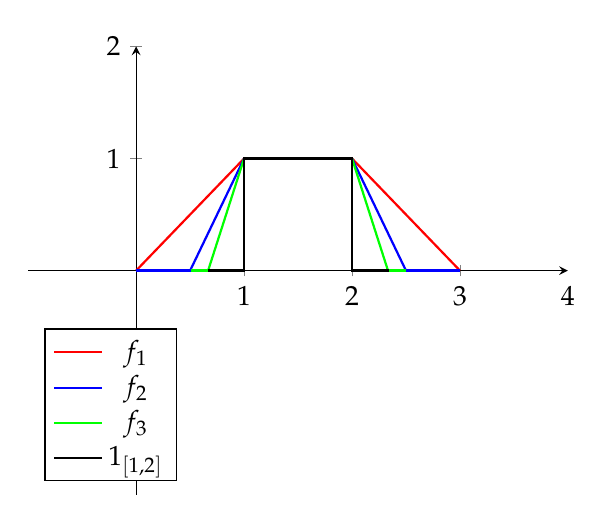
\begin{tikzpicture}\begin{axis}[axis lines = middle, 
xmin=-1,xmax=4,
ymin=-2,ymax=2,     
xtick={0,1,2,3,4},     
ytick={1,2},
legend pos= south west,]


\addplot [domain=0:1,samples=100,color=red,thick] ({x}, {x});
\addplot [domain=0:0.5,samples=100,color=blue,thick] ({x}, {0});
\addplot [domain=0.51:0.666,samples=100,color=green,thick] ({x}, {0});
\addplot [domain=0.666:1,samples=100,color=black,thick] ({x}, {0});


\addplot [domain=1:2,samples=100,color=red,thick] ({x}, {1});
\addplot [domain=2:3,samples=100,color=red,thick] ({x}, {-x + 3});

\addplot [domain=0:0.5,samples=100,color=blue,thick] ({x}, {0});
\addplot [domain=0.5:1,samples=100,color=blue,thick] ({x}, {2*x - 1});
\addplot [domain=1:2,samples=100,color=blue,thick] ({x}, {1});
\addplot [domain=2:2.5,samples=100,color=blue,thick] ({x}, {-2*x + 5});
\addplot [domain=2.5:3,samples=100,color=blue,thick] ({x}, {0});

\addplot [domain=0.51:0.666,samples=100,color=green,thick] ({x}, {0});
\addplot [domain=0.666:1,samples=100,color=green,thick] ({x}, {3*x - 2});
\addplot [domain=1:2,samples=100,color=green,thick] ({x}, {1});
\addplot [domain=2:2.333,samples=100,color=green,thick] ({x}, {-3*x + 7});
\addplot [domain=2.333:2.49,samples=100,color=green,thick] ({x}, {0});

\addplot [domain=0.666:1,samples=100,color=black,thick] ({x}, {0});
\addplot [domain=1:2,samples=100,color=black,thick] ({x}, {1});
\addplot [domain=2:2.333,samples=100,color=black,thick] ({x}, {0});


\node[] (x) at (axis cs:1,-0.1) {$$};
\node[] (y) at (axis cs:1,1.1) {$$};
\node[] (z) at (axis cs:2,-0.1) {$$};
\node[] (w) at (axis cs:2,1.1) {$$};

\draw [color=black,thick] (x) -- (y);
\draw [color=black,thick] (z) -- (w);



\addlegendentry{$ f_1 $} 
\addlegendentry{$ f_2 $}
\addlegendentry{$ f_3 $} 
\addlegendentry{$ 1_{[1,2] }$} 

\end{axis}\end{tikzpicture}\end{center}

For each $n\in\mathbb{N}$, the function $f_{n}$ is continuous since
each of its segments is continuous and are equal on their boundaries.

~~~Let us check that $(f_{n})$ converges pointwise to $1_{I}$:
If $x\in[a,c)$, then we choose $N\in\mathbb{N}$ such that 
\[
x\leq c-\left(\frac{c-a}{N}\right).
\]
Then $f_{n}(x)=0$ for all $n\geq N$. Thus
\[
\lim_{n\to\infty}f_{n}(x)=0=1_{I}(x).
\]

Similarly, if $x\in(d,b]$, then we choose $N\in\mathbb{N}$ such
that
\[
x\geq d+\left(\frac{b-d}{N}\right).
\]
Then $f_{n}(x)=0$ for all $n\geq N$. Thus
\[
\lim_{n\to\infty}f_{n}(x)=0=1_{I}(x).
\]

Finally, if $x\in[c,d]$, then $f_{n}(x)=1$ for all $n\in\mathbb{N}$
by definition and thus
\[
\lim_{n\to\infty}f_{n}(x)=0=1_{I}(x).
\]

~~~Let us check that $(f_{n})$ is Cauchy in $(C[a,b],\|\cdot\|_{1})$.
Let $\varepsilon>0$. Choose $N\in\mathbb{N}$ such that 
\[
\frac{c-a+b-d}{n}<\varepsilon
\]
for all $n\geq N$. Then $n\geq m\geq N$ implies
\begin{align*}
\|f_{n}-f_{m}\|_{1} & =\int_{a}^{b}|f_{n}(x)-f_{m}(x)|\mathrm{d}x\\
 & =\int_{a}^{b}(f_{n}(x)-f_{m}(x))\mathrm{d}x\\
 & =\int_{c-\left(\frac{c-a}{m}\right)}^{c}(f_{n}(x)-f_{m}(x))\mathrm{d}x+\int_{d}^{d+\left(\frac{b-d}{m}\right)}(f_{n}(x)-f_{m}(x))\mathrm{d}x\\
 & \leq\int_{c-\left(\frac{c-a}{m}\right)}^{c}\mathrm{d}x+\int_{d}^{d+\left(\frac{b-d}{m}\right)}\mathrm{d}x\\
 & =\frac{c-a}{m}+\frac{b-d}{m}\\
 & =\frac{c-a+b-d}{m}\\
 & <\varepsilon.
\end{align*}
Thus the sequence $(f_{n})$ is Cauchy in $(C[a,b],\|\cdot\|_{1})$. 

~~~Finally, we check that $\|f_{n}\|_{1}\to\mathrm{length}(I)$
as $n\to\infty$. We have
\begin{align*}
d-c & \leq\|f_{n}\|_{1}\\
 & =\int_{a}^{b}|f_{n}(x)|\mathrm{d}x\\
 & =\int_{a}^{b}f_{n}(x)\mathrm{d}x\\
 & =\int_{c-\left(\frac{c-a}{n}\right)}^{c}f_{n}(x)\mathrm{d}x+\int_{c}^{d}\mathrm{d}x+\int_{d}^{d+\left(\frac{b-d}{n}\right)}f_{n}(x)\mathrm{d}x\\
 & \leq\int_{c-\left(\frac{c-a}{n}\right)}^{c}\mathrm{d}x+\int_{c}^{d}\mathrm{d}x+\int_{d}^{d+\left(\frac{b-d}{n}\right)}\mathrm{d}x\\
 & =\frac{c-a}{n}+d-c+\frac{b-d}{n}\\
 & \to d-c.
\end{align*}
Thus for each $n\in\mathbb{N}$, we have 
\begin{equation}
d-c\leq\|f_{n}\|_{1}\leq d-c+\frac{c-a+b-d}{n}.\label{eq:ineqca-1}
\end{equation}
By taking $n\to\infty$ in (\ref{eq:ineqca-1}), we see that
\begin{align*}
\lim_{n\to\infty}\|f_{n}\|_{1} & =d-c\\
 & =\mathrm{length}(I).
\end{align*}

\hfill

\textbf{Case 2}: Suppose $I=(c,d)$. For each $n\geq2$, define

\[
f_{n}(x)=\begin{cases}
0 & \text{if }a\leq x\leq c\\
\frac{n}{d-c}(x-c) & \text{if }c<x\leq c+\left(\frac{d-c}{n}\right)\\
1 & \text{if }c+\left(\frac{d-c}{n}\right)\leq x\leq d-\left(\frac{d-c}{n}\right)\\
\frac{n}{c-d}(x-d) & \text{if }d-\left(\frac{d-c}{n}\right)\leq x\leq d\\
0 & \text{if }d\leq x\leq b
\end{cases}
\]

The image below gives the graphs for $f_{2}$, $f_{3}$, and $f_{4}$
in the case where $[a,b]=[0,3]$ and $(c,d)=(1,2)$. 

\begin{center}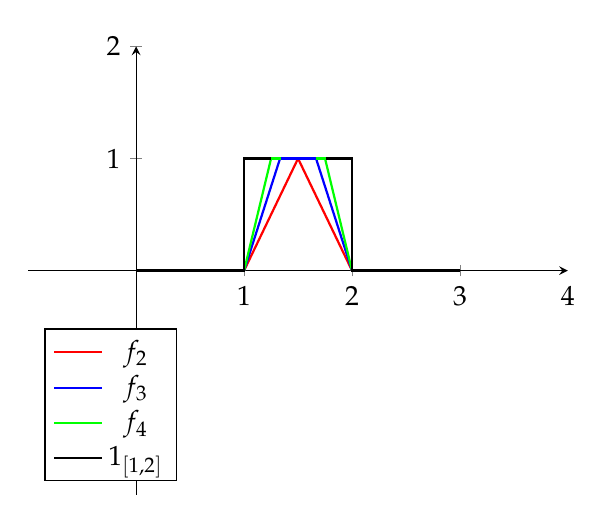
\begin{tikzpicture}\begin{axis}[axis lines = middle, 
xmin=-1,xmax=4,
ymin=-2,ymax=2,     
xtick={0,1,2,3,4},     
ytick={1,2},
legend pos= south west,]



\addplot [domain=0:1,samples=100,color=red,thick] ({x}, {0});
\addplot [domain=0:1,samples=100,color=blue,thick] ({x}, {0});
\addplot [domain=0:1,samples=100,color=green,thick] ({x}, {0});
\addplot [domain=0:1,samples=100,color=black,thick] ({x}, {0});





\addplot [domain=1:1.5,samples=100,color=red,thick] ({x}, {2*x - 2});
\addplot [domain=1.5:2,samples=100,color=red,thick] ({x}, {-2*x +4 });
\addplot [domain=2:3,samples=100,color=red,thick] ({x}, {0});

\addplot [domain=1:1.333,samples=100,color=blue,thick] ({x}, {3*x - 3});
\addplot [domain=1.333:1.666,samples=100,color=blue,thick] ({x}, {1});
\addplot [domain=1.666:2,samples=100,color=blue,thick] ({x}, {-3*x +6 });
\addplot [domain=2:3,samples=100,color=blue,thick] ({x}, {0});

\addplot [domain=1:1.25,samples=100,color=green,thick] ({x}, {4*x - 4});
\addplot [domain=1.25:1.333,samples=100,color=green,thick] ({x}, {1});
\addplot [domain=1.666:1.75,samples=100,color=green,thick] ({x}, {1});
\addplot [domain=1.75:2,samples=100,color=green,thick] ({x}, {-4*x +8 });
\addplot [domain=2:3,samples=100,color=green,thick] ({x}, {0});

\addplot [domain=1:1.24,samples=100,color=black,thick] ({x}, {1});
\addplot [domain=1.76:2,samples=100,color=black,thick] ({x}, {1});
\addplot [domain=2:3,samples=100,color=black,thick] ({x}, {0});


\node[] (x) at (axis cs:1,-0.1) {$$};
\node[] (y) at (axis cs:1,1.1) {$$};
\node[] (z) at (axis cs:2,-0.1) {$$};
\node[] (w) at (axis cs:2,1.1) {$$};

\draw [color=black,thick] (x) -- (y);
\draw [color=black,thick] (z) -- (w);


\addlegendentry{$ f_2 $} 
\addlegendentry{$ f_3 $}
\addlegendentry{$ f_4 $} 
\addlegendentry{$ 1_{[1,2] }$} 



\end{axis}\end{tikzpicture}\end{center}

That $(f_{n})$ is a Cauchy sequence of continuous funtions in $(C[a,b],\|\cdot\|_{1})$
which converges pointwise to $1_{I}$ and $\|f_{n}\|_{1}\to\mathrm{length}(I)$
as $n\to\infty$ follows from similar arguments used in case 1. \end{proof} 

\subsection{Algebra of Subsets of $X$ Closed under Symmetric Differenences and
Relative Compliments}

\begin{prop}\label{prop} Let $\mathcal{A}$ be an algebra of subsets
of $X$. Then
\begin{enumerate}
\item $\mathcal{A}$ is closed under finite unions: if $A,B\in\mathcal{A}$,
then $A\cup B\in\mathcal{A}$.
\item $\mathcal{A}$ is closed under relative compliments: if $A,B\in\mathcal{A}$,
then $A\backslash B\in\mathcal{A}$.
\item $\mathcal{A}$ is closed under symmetric differences: if $A,B\in\mathcal{A}$,
then $A\Delta B\in\mathcal{A}$.
\end{enumerate}
\end{prop}

\begin{proof}\label{proof}\hfill

1. Let $A,B\in\mathcal{A}$. Then
\begin{align*}
A\cup B & =((A\cup B)^{c})^{c}\\
 & =(A^{c}\cap B^{c})^{c}\\
 & \in\mathcal{A}.
\end{align*}

\hfill

2. Let $A,B\in\mathcal{A}$. Then
\begin{align*}
A\backslash B & =A\cap B^{c}\\
 & \in\mathcal{A}.
\end{align*}

\hfill

3. Let $A,B\in\mathcal{A}$. Then it follows from 1 and 2 that
\begin{align*}
A\Delta B & =(A\backslash B)\cup(B\backslash A)\\
 & \in\mathcal{A}.
\end{align*}

\end{proof}

\subsection{Collection of all Subintervals of $[a,b]$ Forms a Semialgebra}

\begin{defn}\label{defn} A nonempty collection $\mathcal{E}$ of
subsets of $X$ is said to be a \textbf{semialgebra }of sets if it
satisfies the following properties:
\begin{enumerate}
\item $\emptyset\in\mathcal{E}$;
\item If $E,F\in\mathcal{E}$, then $E\cap F\in\mathcal{E}$;
\item If $E\in\mathcal{E}$, then $E^{c}$ is a finite disjoint union of
sets from $\mathcal{E}$. 
\end{enumerate}
\end{defn}

\subsection*{Problem 4.a}

\begin{prop}\label{prop} The collection of all subintervals of $[a,b]$
forms a semialgebra of sets. \end{prop}

\begin{proof} Let $\mathcal{I}$ denote the collection of all subintervals
of $[a,b]$. We have $\emptyset\in\mathcal{I}$ since $\emptyset=(c,c)$
for any $c\in[a,b]$. 

~~~Now we show $\mathcal{I}$ is closed under finite intersections.
Let $I_{1}$ and $I_{2}$ be subintervals of $[a,b]$. Taking the
closure of $I_{1}$ and $I_{2}$ gives us closed intervals, say
\[
\overline{I}_{1}=[c_{1},d_{1}]\quad\text{and}\quad\overline{I}_{2}=[c_{2},d_{2}].
\]

Assume without loss of generality that $c_{1}\leq c_{2}$. If $d_{1}<c_{2}$,
then $I_{1}\cap I_{2}=\emptyset$, so assume that $d_{1}\geq c_{2}$.
If $d_{1}\geq d_{2}$, then $I_{1}\cap I_{2}=I_{2}$, so assume that
$d_{1}<d_{2}$. If $c_{1}=c_{2}$, then $I_{1}\cap I_{2}=I_{1}$,
so assume that $c_{2}>c_{1}$. So we have reduced the case to where
\[
c_{1}<c_{2}\leq d_{1}<d_{2}.
\]

With these assumptions in mind, we now consider four cases:

\hfill

\textbf{Case 1: }If\textbf{ $I_{1}=[c_{1},d_{1}]$ }or $I_{1}=(c_{1},d_{1}]$\textbf{
}and $I_{2}=[c_{2},d_{2}]$ or $I_{2}=[c_{2},d_{2})$, then $I_{1}\cap I_{2}=[c_{2},d_{1}]$.

\hfill

\textbf{Case 2: }If\textbf{ $I_{1}=[c_{1},d_{1})$ }or $I_{1}=(c_{1},d_{1})$\textbf{
}and $I_{2}=[c_{2},d_{2}]$ or $I_{2}=[c_{2},d_{2})$, then $I_{1}\cap I_{2}=[c_{2},d_{1})$.

\hfill

\textbf{Case 3: }If\textbf{ $I_{1}=[c_{1},d_{1}]$ }or $I_{1}=(c_{1},d_{1})$\textbf{
}and $I_{2}=(c_{2},d_{2}]$ or $I_{2}=(c_{2},d_{2})$, then $I_{1}\cap I_{2}=(c_{2},d_{1})$.

\hfill

\textbf{Case 4: }If\textbf{ $I_{1}=[c_{1},d_{1})$ }or $I_{1}=(c_{1},d_{1})$\textbf{
}and $I_{2}=(c_{2},d_{2}]$ or $I_{2}=(c_{2},d_{2})$, then $I_{1}\cap I_{2}=(c_{2},d_{1})$.

\hfill

In all cases, we see that $I_{1}\cap I_{2}$ is a subinterval of $[a,b]$. 

~~~Now we show that compliments can be expressed as finite disjoint
unions. Let $I$ be a subinterval of $[a,b]$ and write $\overline{I}=[c,d]$.
We consider four cases:

\hfill

\textbf{Case 1: }If $I=[c,d]$, then $I^{c}=[a,c)\cup(d,b]$.

\hfill

\textbf{Case 2: }If $I=(c,d]$, then $I^{c}=[a,c]\cup(d,b]$.

\hfill

\textbf{Case 3: }If $I=[c,d)$, then $I^{c}=[a,c)\cup[d,b]$.

\hfill

\textbf{Case 4: }If $I=(c,d)$, then $I^{c}=[a,c]\cup[d,b]$.

\hfill

Thus in all cases, we can express $I^{c}$ as a disjoint union of
intervals since $a\leq c\leq d\leq b$. 

\end{proof}

\subsection*{Problem 4.b}

\begin{prop}\label{prop} Let $\mathcal{I}$ be the collection of
all subintervals of $\mathbb{R}\cup\{\infty\}$ of the form $(a,b]$.
Then $\mathcal{I}$ forms a semialgebra of sets. \end{prop}

\begin{proof} We have $\emptyset\in\mathcal{I}$ since $\emptyset=(c,c]$
for any $c\in\mathbb{R}\cup\{\infty\}$. 

~~~Now we show $\mathcal{I}$ is closed under finite intersections.
Let $I_{1}=(c_{1},d_{1}]$ and $I_{2}=(c_{2},d_{2}]$. Assume without
loss of generality that $c_{1}\leq c_{2}$. Then
\begin{align*}
I_{1}\cap I_{2} & =\begin{cases}
(c_{2},d_{1}] & \text{if }c_{2}\leq d_{1}\\
\emptyset & \text{else}
\end{cases}
\end{align*}

~~~Now we show that compliments can be expressed as finite disjoint
unions. Let $I=(c,d]$. Then
\begin{align*}
I^{c} & =(-\infty,c]\cup(d,\infty],
\end{align*}
where the union is disjoint since $c\leq d$. \end{proof}

\subsection*{Problem 4.c}

\begin{prop}\label{prop} Let $\mathcal{E}$ be a semialgebra of sets.
Then the collection $\mathcal{A}$ consisting of all sets which are
finite disjoint union of sets in $\mathcal{E}$ forms an algebra of
sets. \end{prop}

\begin{proof} We have $\emptyset\in\mathcal{A}$ since $\emptyset\in\mathcal{E}$.

~~~Next we show that $\mathcal{A}$ is closed under finite intersections.
Let $A,A'\in\mathcal{A}$. Express $A$ and $A'$ as a disjoint union
of members of $\mathcal{E}$, say
\[
A=E_{1}\cup\cdots\cup E_{n}\quad\text{and}\quad A'=E'_{1}\cup\cdots\cup E'_{n'}.
\]
Then we have
\begin{align*}
A\cap A' & =\left(\bigcup_{i=1}^{n}E_{i}\right)\cap\left(\bigcup_{i'=1}^{n'}E'_{i'}\right)\\
 & =\bigcup_{i'=1}^{n'}\left(\left(\bigcup_{i=1}^{n}E_{i}\right)\cap E'_{i'}\right)\\
 & =\bigcup_{i'=1}^{n'}\left(\bigcup_{i=1}^{n}E_{i}\cap E'_{i'}\right)\\
 & =\bigcup_{\substack{1\leq i\leq n\\
1\leq i'\leq n'
}
}E_{i}\cap E'_{i'}
\end{align*}
where the union is disjoint since the $E_{i}$ and $E'_{i'}$ are
disjoint from one another. 

~~~Lastly we show that $\mathcal{A}$ is closed under compliments.
Let $A\in\mathcal{A}$. Express $A$ as a disjoint union of members
of $\mathcal{E}$, say
\[
A=E_{1}\cup\cdots\cup E_{n}.
\]
Then we have
\begin{align*}
A^{c} & =(E_{1}\cup\cdots\cup E_{n})^{c}\\
 & =E_{1}^{c}\cap\cdots\cap E_{n}^{c}.
\end{align*}
Since the $E_{i}^{c}$ belong to $\mathcal{A}$ and $\mathcal{A}$
is closed under finite intersections, it follows that $A^{c}\in\mathcal{A}$.
\end{proof}

\subsection{Collection of Subsets of $\mathbb{Z}$ Forms Algebra Under Certain
Conditions}

\begin{prop}\label{prop} Let $\mathcal{A}$ be a collection of subsets
of $\mathbb{Z}$ such that
\begin{enumerate}
\item $X$ is a member of $\mathcal{A}$;
\item $\mathcal{A}$ is closed under relative compliments: $A\backslash B\in\mathcal{A}$
for all $A,B\in\mathcal{A}$. 
\end{enumerate}
Then $\mathcal{A}$ is an algebra. \end{prop}

\begin{proof} We have $\emptyset\in\mathcal{A}$ since $\emptyset=X\backslash X\in\mathcal{A}$.
Clearly $\mathcal{A}$ is closed under compliments since it is closed
under relative compliments, so we just need to show that $\mathcal{A}$
is closed under finite intersections. Let $A,B\in\mathcal{A}$. Then
\begin{align*}
A\cap B & =A\cap(B^{c})^{c}\\
 & =A\backslash B^{c}\\
 & \in\mathcal{A}.
\end{align*}

\end{proof}

\subsection{Finite Complement Algebra}

\begin{prop}\label{prop} Let $\mathcal{A}$ be the collection of
subsets of $X$ which satisfies the property that if $A\in\mathcal{A}$
then either $A$ or $A^{c}$ is finite. Then $\mathcal{A}$ forms
an algebra. \end{prop}

\begin{proof} We have $\emptyset\in\mathcal{A}$ since $\emptyset$
is finite. Clearly $\mathcal{A}$ is closed under compliments since
$A\in\mathcal{A}$ implies either $A$ or $A^{c}$ is finite which
implies $A^{c}\in\mathcal{A}$. It remains to show that $\mathcal{A}$
is closed under finite intersections. Let $A,B\in\mathcal{A}$ and
suppose that $A\cap B$ is infinite. We must show that $(A\cap B)^{c}=A^{c}\cup B^{c}$
is finite. In other words, we need to show that both $A^{c}$ and
$B^{c}$ are finite. Assume for a contradiction that $A^{c}$ is infinite.
Then $A$ must be finite since $A\in\mathcal{A}$. But this implies
$A\cap B$ is finite, which is a contradiction. Thus $A^{c}$ must
be finite. Similarly, we can prove by contradiction that $B^{c}$
is finite too. \end{proof}

\subsection{Ascending Sequence of Algebras is an Algebra}

\begin{prop}\label{prop} Let $(\mathcal{A}_{n})$ be an ascending
sequence of algebras over $X$, that is, $\mathcal{A}_{n}$ is an
algebra of subsets of $X$ and $\mathcal{A}_{n}\subseteq\mathcal{A}_{n+1}$
for all $n\in\mathbb{N}$. Then
\[
\mathcal{A}:=\bigcup_{n\in\mathbb{N}}\mathcal{A}_{n}
\]
is an algebra. \end{prop}

\begin{proof} We have $\emptyset\in\mathcal{A}$ since $\emptyset\in A_{1}\subseteq\mathcal{A}$.
Next we show that $\mathcal{A}$ is closed under finite intersections.
Let $A,B\in\mathcal{A}$. Then $A\in A_{i}$ and $B\in\mathcal{A}_{j}$
for some $i,j\in\mathbb{N}$. Without loss of generality, assume that
$i\leq j$. Then $A\in\mathcal{A}_{i}\subseteq\mathcal{A}_{j}$. Thus
$A\cap B\in\mathcal{A}_{j}\subseteq\mathcal{A}$. Lastly we show that
$\mathcal{A}$ is closed under compliments. Let $A\in\mathcal{A}$.
Then $A\in A_{i}$ for some $i\in\mathbb{N}$. Thus $A^{c}\in\mathcal{A}_{i}\subseteq\mathcal{A}$.
\end{proof}

\begin{rem}\label{rem} The ascending condition is not necessary.
Indeed, consider $X=\{a,b,c\}$ and
\begin{align*}
\mathcal{A} & =\{\emptyset,X,\{a\},\{b,c\}\}\\
\mathcal{B} & =\{\emptyset,X,\{b\},\{a,c\}\}\\
\mathcal{C} & =\{\emptyset,X,\{c\},\{a,b\}\}
\end{align*}
Then $\mathcal{A}$, $\mathcal{B}$, and $\mathcal{C}$ are algebras
over $X$, and $\mathcal{A}\cup\mathcal{B}\cup\mathcal{C}=\mathcal{P}(X)$
is an algebra over $X$, but none of the $\mathcal{A}$, $\mathcal{B}$,
or $\mathcal{C}$ contain one another. \end{rem}

\section{Homework 2}

Throughout this homework, let $(X,\mathcal{M},\mu)$ be a measure
space. We say that $(X,\mathcal{M},\mu)$ is a \textbf{finite }measure
space if $\mu(X)<\infty$. Observe that in this case, we have $\mu(A)<\infty$
for all $A\in\mathcal{M}$, by monotonicity of $\mu$. 

\subsection{Countable Subadditivity of Finite Measure}

\begin{prop}\label{prop} Let $(E_{n})$ be a sequence of sets in
$\mathcal{M}$. Then
\[
\mu\left(\bigcup_{n=1}^{\infty}E_{n}\right)\leq\sum_{n=1}^{\infty}\mu(E_{n})
\]

\end{prop}

\begin{proof} Disjointify\footnote{See Appendix for details on disjointification.}
$(E_{n})$ into the sequence $(D_{n})$; set $D_{1}:=E_{1}$ and 
\[
D_{n}:=E_{n}\backslash\left(\bigcup_{i=1}^{n-1}E_{n}\right)
\]
for all $n>1$. Then we have
\begin{align*}
\mu\left(\bigcup_{n=1}^{\infty}E_{n}\right) & =\mu\left(\bigcup_{n=1}^{\infty}D_{n}\right)\\
 & =\sum_{n=1}^{\infty}\mu(D_{n})\\
 & \leq\sum_{n=1}^{\infty}\mu(E_{n}),
\end{align*}
where we use countable additivity of $\mu$ to get from the first
line to the second line and where we used monotonicity of $\mu$ to
get from the second line to the third line. \end{proof}

\subsection{Inverse Image of $\sigma$-Algebra is $\sigma$-Algebra}

\begin{prop}\label{proppullbacksemialgebra} Let $(Y,\mathcal{N},\nu)$
be a measure space and suppose $f\colon X\to Y$ is a function. Then
$(X,f^{-1}(\mathcal{N}),f^{-1}\mu)$ is a measure space, where
\[
f^{-1}(\mathcal{N})=\{f^{-1}(B)\subseteq X\mid B\in\mathcal{N}\}
\]
and where $f^{-1}\mu\colon f^{-1}(\mathcal{N})\to[0,\infty]$ is defined
by
\[
(f^{-1}\mu)(A)=\mu^{*}(f(A)).
\]
for all $A\in f^{-1}(\mathcal{N})$. \end{prop}

\begin{proof} We first show that $f^{-1}(\mathcal{N})$ is a $\sigma$-algebra.
This follows from the fact that $f^{-1}$ commutes with unions and
compliments: 
\[
f^{-1}\left(\bigcup_{j\in J}B_{j}\right)=\bigcup_{j\in J}f^{-1}\left(B_{j}\right)\quad\text{and}\quad f^{-1}\left(Y\backslash B\right)=f^{-1}(Y)\backslash f^{-1}(B)
\]
for all subsets $B$ and $B_{j}$ of $Y$ for all $j\in J$. Indeed,
we have 
\begin{align*}
x\in\bigcup_{j\in J}f^{-1}\left(B_{j}\right) & \iff x\in f^{-1}(B_{j})\text{ for some }j\in J\\
 & \iff f(x)\in B_{j}\text{ for some }j\in J\\
 & \iff f(x)\in\bigcup_{j\in J}B_{j}\\
 & \iff x\in f^{-1}\left(\bigcup_{j\in J}B_{j}\right)
\end{align*}

and we have
\begin{align*}
x\in f^{-1}\left(Y\backslash B\right) & \iff f(x)\in Y\backslash B\\
 & \iff f(x)\in Y\text{ and }f(a)\notin B\\
 & \iff x\in f^{-1}(Y)\text{ and }a\notin f^{-1}(B)\\
 & \iff x\in f^{-1}(Y)\backslash f^{-1}(B).
\end{align*}

~~~Now we show that the function $f^{*}\mu$ is a measure. We have
\begin{align*}
(f^{-1}\mu)(\emptyset) & =\inf\{\mu(B)\mid f(\emptyset)\subset B\}\\
 & =\inf\{\mu(B)\mid\emptyset\subset B\}\\
 & \leq\mu(\emptyset)\\
 & =0.
\end{align*}
Next, let $(A_{n})$ be a sequence of members of $f^{-1}(\mathcal{N})$.
Then 
\begin{align*}
(f^{-1}\mu)\left(\bigcup_{n=1}^{\infty}A_{n}\right) & =\mu^{*}\left(f\left(\bigcup_{n=1}^{\infty}A_{n}\right)\right)\\
 & =\mu^{*}\left(\bigcup_{n=1}^{\infty}f(A_{n})\right)\\
 & \leq\sum_{n=1}^{\infty}\mu^{*}(f(A_{n}))\\
 & =\sum_{n=1}^{\infty}(f^{-1}\mu)(A_{n}).
\end{align*}
Thus $f^{-1}\mu$ is countably subadditive. 

~~~Finally, let $A$ and $A'$ be two members in $f^{-1}(\mathcal{N})$
such that $A\cap A'=\emptyset$. Then
\begin{align*}
(f^{-1}\mu)(A\cup A') & =\mu^{*}(f(A)\cup f(A'))\\
 & =\\
 & =
\end{align*}

. \end{proof}

~~~We first show that
\[
\sum_{n=1}^{\infty}\inf\left\{ \mu(B_{n})\mid f(A_{n})\subset B_{n}\right\} \leq\inf\left\{ \mu(B)\mid\bigcup_{n=1}^{\infty}f(A_{n})\subset B\right\} .
\]
Let $\varepsilon>0$. Choose $ $

\subsection{Locally Measurable Sets}

\begin{defn}\label{defn} A set $E\subseteq X$ is called \textbf{locally
measurable }if $E\cap A\in\mathcal{M}$ for all $A\in\mathcal{M}$
with finite measure. \end{defn}

\begin{prop}\label{prop} Suppose $(X,\mathcal{M},\mu)$ is a finite
measure space. Let $\widetilde{\mathcal{M}}$ be the collection of
all locally measurable subsets of $X$. Then $\mathcal{M}=\widetilde{\mathcal{M}}$.
\end{prop}

\begin{proof} Let first show that $\mathcal{M}\subseteq\widetilde{\mathcal{M}}$.
Let $E\in\mathcal{M}$. Then $E\cap A\in\mathcal{M}$ for all $A\in\mathcal{M}$
since $\mathcal{M}$ is closed under finite intersections. In particular,
this implies $E\in\widetilde{\mathcal{M}}$. Thus $\mathcal{M}\subseteq\widetilde{\mathcal{M}}$.

~~~Now we show the reverse inclusion $\mathcal{M}\supseteq\widetilde{\mathcal{M}}$.
Let $E\in\widetilde{\mathcal{M}}$. Since $\mu(X)<\infty$ and $E$
is locally measurable, we have
\begin{align*}
E & =E\cap X\\
 & \in\mathcal{M}.
\end{align*}
Thus $\mathcal{M}\supseteq\widetilde{\mathcal{M}}$. \end{proof}

\subsection{If $\mu(A)<\infty$, then $\mu(B\backslash A)=\mu(B)-\mu(A)$}

\begin{lemma}\label{lemmameasuredif} Let $A,B\in\mathcal{M}$ such
that $A\subseteq B$. If $\mu(A)<\infty$, then 
\[
\mu(B\backslash A)=\mu(B)-\mu(A).
\]
\end{lemma}

\begin{proof} By finite additivity of $\mu$, we have 
\begin{align*}
\mu(B) & =\mu((B\backslash A)\cup A)\\
 & =\mu(B\backslash A)+\mu(A).
\end{align*}
If moreover $\mu(A)<\infty$, then we may subtract $\mu(A)$ from
both sides to obtain 
\[
\mu(B\backslash A)=\mu(B)-\mu(A).
\]
\end{proof}

\subsection*{Problem 4.a}

\begin{prop}\label{prop} Suppose $(X,\mathcal{M},\mu)$ is a finite
measure space. Then
\[
\mu(A\cup B)+\mu(A\cap B)=\mu(A)+\mu(B).
\]

for all $A,B\in\mathcal{M}$.\end{prop}

\begin{proof} Let $A,B\in\mathcal{M}$. Then by finite additivity
of $\mu$, we have
\begin{align*}
\mu(A\cup B) & =\mu(A\cup(B\backslash A))\\
 & =\mu(A)+\mu(B\backslash A)\\
 & =\mu(A)+\mu(B\backslash(A\cap B))\\
 & =\mu(A)+\mu(B)-\mu(A\cap B),
\end{align*}
where the last equality follows Lemma~(\ref{lemmameasuredif}) since
$(X,\mathcal{M},\mu)$ is a finite measure space. \end{proof}

\subsection{Countable Additivity of $\mu$ for ``Almost Pairwise Disjoint''
Sets}

\begin{prop}\label{prop} Let $(A_{n})$ be a sequence of ``almost
pairwise disjoint'' members of $\mathcal{M}$, in the sense that
$\mu(A_{i}\cap A_{j})=0$ whenever $i\neq j$. Then
\[
\mu\left(\bigcup_{n=1}^{\infty}A_{n}\right)=\sum_{n=1}^{\infty}\mu(A_{n}).
\]
\end{prop}

\begin{proof} First note that countable subadditivity of $\mu$ implies
\[
\mu\left(\bigcup_{n=1}^{\infty}A_{n}\right)\leq\sum_{n=1}^{\infty}\mu(A_{n}),
\]
so it suffices to show the reverse inequality. Before doing so, we
first prove by induction on $N\geq1$, that
\begin{equation}
\mu\left(\bigcup_{n=1}^{N}A_{n}\right)=\sum_{n=1}^{N}\mu(A_{n}).\label{eq:almostpairwisedisjoint}
\end{equation}
The base case $N=1$ holds trivially. Assume that we have shown (\ref{eq:almostpairwisedisjoint})
holds for some $N>1$. Then
\begin{align*}
\mu\left(\bigcup_{n=1}^{N+1}A_{n}\right) & =\mu\left(\left(\bigcup_{n=1}^{N}A_{n}\right)\cup A_{N+1}\right)\\
 & =\mu\left(\bigcup_{n=1}^{N}A_{n}\right)+\mu(A_{N+1})-\mu\left(\left(\bigcup_{n=1}^{N}A_{n}\right)\cap A_{N+1}\right)\\
 & =\sum_{n=1}^{N}\mu\left(A_{N}\right)+\mu(A_{N+1})-\mu\left(\bigcup_{n=1}^{N}(A_{n}\cap A_{N+1})\right)\\
 & \geq\sum_{n=1}^{N+1}\mu(A_{n})-\sum_{n=1}^{N}\mu(A_{n}\cap A_{N+1})\\
 & =\sum_{n=1}^{N+1}\mu(A_{n})-\sum_{n=1}^{N}0\\
 & =\sum_{n=1}^{N+1}\mu(A_{n}),
\end{align*}
where we used the induction hypothesis to get from the second line
to the third line, and where we used finite subadditivity of $\mu$
to get from the third line to the fourth line. We already have
\[
\mu\left(\bigcup_{n=1}^{N+1}A_{n}\right)\leq\sum_{n=1}^{N+1}\mu(A_{n})
\]
by finite subadditivity of $\mu$, and so it follows that
\[
\mu\left(\bigcup_{n=1}^{N+1}A_{n}\right)=\sum_{n=1}^{N+1}\mu(A_{n}).
\]
Therefore (\ref{eq:almostpairwisedisjoint}) holds for all $N\in\mathbb{N}$
induction. 

~~~Now we prove the reverse inequality: for each $N\in\mathbb{N}$,
we have 
\begin{align*}
\sum_{n=1}^{N}\mu(A_{n}) & =\mu\left(\bigcup_{n=1}^{N}A_{n}\right)\\
 & \subseteq\mu\left(\bigcup_{n=1}^{\infty}A_{n}\right)
\end{align*}
by monotonicity of $\mu$. By taking $N\to\infty$, we see that
\[
\sum_{n=1}^{\infty}\mu(A_{n})\leq\mu\left(\bigcup_{n=1}^{\infty}A_{n}\right).
\]

\end{proof} 

\subsection{Nonuniqueness of Extension of Algebra to $\sigma$-Algebra}

\begin{prop}\label{prop} Let $\mathcal{A}$ be the collection of
all finite unions of sets of the form $(a,b]\cap\mathbb{Q}$ where
$-\infty\leq a\leq b\leq\infty$. Then
\begin{enumerate}
\item $\mathcal{A}$ is an algebra of subsets of $\mathbb{Q}$;
\item $\sigma(\mathcal{A})=\mathcal{P}(\mathbb{Q})$ where $\mathcal{P}(\mathbb{Q})$
is the collection of all subsets of $\mathbb{Q}$;
\item the function $\mu\colon\mathcal{A}\to[0,\infty]$ defined by $\mu(\emptyset)=0$
and $\mu(A)=\infty$ for all nonempty $A\in\mathcal{A}$ is a measure
on $\mathcal{A}$;
\item there is more than one measure on $\sigma(\mathcal{A})$ whose restriction
to $\mathcal{A}$ is $\mu$;
\end{enumerate}
\end{prop}

\begin{proof} \hfill

1. In Homework 1, it was shown that $(\mathbb{R}\cup\{\infty\},\mathcal{T})$
was a semialgebra, where $\mathcal{T}$ consisted of all subintervals
of $\mathbb{R}\cup\{\infty\}$ of the form $(a,b]$ where $-\infty\leq a\leq b\leq\infty$.
If we let $\iota\colon\mathbb{Q}\to\mathbb{R}\cup\{\infty\}$ denote
the inclusion map, then we see that $\iota^{-1}(\mathcal{T})=\mathcal{S}$,
where $\mathcal{S}$ denotes the collection of all subintervals of
$\mathbb{Q}$ of the form $(a,b]\cap\mathbb{Q}$. It follows easily
from Proposition~(\ref{proppullbacksemialgebra}) that $\mathcal{S}$
is a semialgebra of subsets of $\mathbb{Q}$.\footnote{Technically we showed that the inverse image of a $\sigma$-algebra
is a $\sigma$-algebra. However the same reasoning used in that proof
shows that the inverse image of a semialgebra is a semialgebra: namely
$f^{-1}$ commutes with complements and unions.}

Therefore the set of all finite disjoint unions of members of $\mathcal{S}$
forms an algebra, and as any finite union of members of $\mathcal{S}$
can be expressed as a finite disjoint union of members of $\mathcal{S}$
(since $\mathcal{S}$ is a semialgebra), we see that $\mathcal{A}$
is an algebra.

\hfill

2. Clearly $\mathcal{P}(\mathbb{Q})\supseteq\sigma(\mathcal{A})$.
Let us prove the reverse inclusion. We first observe that $\{r\}\in\sigma(\mathcal{A})$
for all $r\in\mathbb{Q}$. Indeed, if $r\in\mathbb{Q}$, then we have
\begin{align*}
\{r\} & =\bigcap_{n\in\mathbb{N}}(r-1/n,r]\cap\mathbb{Q}\in\sigma(\mathcal{A})
\end{align*}
Now let $S\in\mathcal{P}(\mathbb{Q})$. Then since $S$ is countable,
we have
\begin{align*}
S & =\bigcup_{s\in S}\{s\}\in\sigma(\mathcal{A}).
\end{align*}

\hfill

3. We have $\mu(\emptyset)=0$ by definition. Let $(A_{n})$ be a
sequence of pairwise disjoint members of $\mathcal{A}$ whose union
also belongs to $\mathcal{A}$. If $\bigcup_{n=1}^{\infty}A_{n}\neq\emptyset$,
then $A_{n}\neq\emptyset$ for some $n\in\mathbb{N}$, and thus
\begin{align*}
\mu\left(\bigcup_{n=1}^{\infty}A_{n}\right) & =\infty\\
 & =\mu(A_{n})\\
 & =\sum_{n=1}^{\infty}\mu(A_{n}).
\end{align*}
Similarly, if $\bigcup_{n=1}^{\infty}A_{n}=\emptyset$, then $A_{n}=\emptyset$
for all $n\in\mathbb{N}$, and thus 
\begin{align*}
\mu\left(\bigcup_{n=1}^{\infty}A_{n}\right) & =0\\
 & =\sum_{n=1}^{\infty}0\\
 & =\sum_{n=1}^{\infty}\mu(A_{n}).
\end{align*}
In both cases, we have 
\[
\mu\left(\bigcup_{n=1}^{\infty}A_{n}\right)=\sum_{n=1}^{\infty}\mu(A_{n})
\]

\hfill

4. We define $\mu_{1}\colon\mathcal{P}(\mathbb{Q})\to[0,\infty]$
and $\mu_{2}\colon\mathcal{P}(\mathbb{Q})\to[0,\infty${]} by
\[
\mu_{1}(A)=\begin{cases}
|A| & \text{if }A\text{ is finite}\\
\infty & \text{else}
\end{cases}\quad\text{and}\quad\mu_{2}(A)=\begin{cases}
0 & \text{if }A=\emptyset\\
\infty & \text{if }A\neq\emptyset
\end{cases}
\]
for all $A\in\mathcal{P}(\mathbb{Q})$. Both $\mu_{1}$ and $\mu_{2}$
restrict to $\mu$ as functions since every member of $\mathcal{A}$
is infinite. They are also both distinct as functions since, for example,
$\mu_{1}(\{x\})=1$ and $\mu_{2}(\{x\})=\infty$ for any $x\in\mathbb{Q}$.
Thus it suffices to show that they are measures. That $\mu_{2}$ is
a measure follows from a similar argument as in the case of $\mu$,
so we just show that $\mu_{1}$ is a measure. We have $\mu_{1}(\emptyset)=0$
since $|\emptyset|=0$. Next we show it is finitely additive. Let
$A$ and $B$ be members of $\mathcal{P}(\mathbb{Q})$ such that $A\cap B=\emptyset$.
If $A=\emptyset$, then
\begin{align*}
\mu_{1}(A\cup B) & =\mu_{1}(\emptyset\cup B)\\
 & =\mu_{1}(B)\\
 & =0+\mu_{1}(B)\\
 & =\mu_{1}(\emptyset)+\mu_{1}(B)\\
 & =\mu_{1}(A)+\mu_{1}(B).
\end{align*}
Similarly, if $B=\emptyset$, then $\mu_{1}(A\cup B)=\mu_{1}(A)\cup\mu_{1}(B)$.
So assume neither $A$ nor $B$ is the emptyset. Write them as
\[
A=\{x_{1},\dots x_{m}\}\quad\text{and}\quad B=\{y_{1},\dots,y_{n}\}.
\]
Then 
\[
A\cup B=\{x_{1},\dots,x_{m},y_{1},\dots,y_{n}\},
\]
and so
\begin{align*}
\mu_{1}(A\cup B) & =m+n\\
 & =\mu_{1}(A)+\mu_{1}(B).
\end{align*}
It follows that $\mu_{1}$ is finitely additive. 

~~~Now, let $(A_{n})$ be a sequence of pairwise disjoint members
of $\mathcal{P}(\mathbb{Q})$. Suppose that $A_{n}\neq\emptyset$
for only finitely many $n$, say $n_{1},\dots,n_{k}$. Then it follows
from finite additivity of $\mu_{1}$ and the fact that $\mu(\emptyset)=0$
that
\begin{align*}
\mu_{1}\left(\bigcup_{n=1}^{\infty}A_{n}\right) & =\mu_{1}\left(\bigcup_{i=1}^{k}A_{n_{i}}\right)\\
 & =\sum_{i=1}^{k}\mu(A_{n_{i}})\\
 & =\sum_{n=1}^{\infty}\mu(A_{n}).
\end{align*}
Now suppose that $A_{n}\ne\emptyset$ for infinitely many $n$. By
taking a subsequence of $(A_{n})$ if necessary, we may assume that
$A_{n}\neq\emptyset$ for all $n$. Then $\bigcup_{n=1}^{\infty}A_{n}$
is infinite, and so
\begin{align*}
\mu_{1}\left(\bigcup_{n=1}^{\infty}A_{n}\right) & =\infty\\
 & \geq\sum_{n=1}^{\infty}\mu_{1}(A_{n})\\
 & \geq\sum_{n=1}^{\infty}1\\
 & =\infty.
\end{align*}
It follows that 
\[
\mu_{1}\left(\bigcup_{n=1}^{\infty}A_{n}\right)=\infty=\sum_{n=1}^{\infty}\mu_{1}(A_{n}).
\]
Therefore $\mu_{1}$ and $\mu_{2}$ are distinct measures which restrict
to $\mu$. \end{proof}

\begin{rem}\label{rem} Note that the extension theorem does not apply
here as $\mu$ is not a finite measure. \end{rem}

\subsection{Symmetric Difference Identities}

\begin{prop}\label{prop} Let $A,B\in\mathcal{P}(X)$. Then the following
properties hold
\begin{enumerate}
\item $A\Delta A=\emptyset$;
\item $(A\Delta B)\Delta C=A\Delta(B\Delta C)$;
\item $(A\Delta B)\Delta(B\Delta C)=A\Delta C$;
\item $(A\Delta B)\Delta(C\Delta D)=(A\Delta C)\Delta(B\Delta D)$;
\item $|1_{A}-1_{B}|=1_{A\Delta B}$.
\end{enumerate}
\end{prop}

\begin{proof}\hfill

1. We have
\begin{align*}
A\Delta A & =(A\backslash A)\cup(A\backslash A)\\
 & =\emptyset\cup\emptyset\\
 & =\emptyset.
\end{align*}

\hfill

2. We have
\begin{align*}
(A\Delta B)\Delta C & =((A\Delta B)\cup C)\cap((A\Delta B)\cap C)^{c}\\
 & =((A\Delta B)\cup C)\cap((A\Delta B)^{c}\cup C^{c})\\
 & =(((A\cup B)\cap(A\cap B)^{c})\cup C))\cap((A\cap B^{c})\cup(A^{c}\cap B))^{c}\cup C^{c})\\
 & =(((A\cup B)\cap(A^{c}\cup B^{c}))\cup C))\cap(((A\cap B^{c})^{c}\cap(A^{c}\cap B)^{c})\cup C^{c})\\
 & =(A\cup B\cup C)\cap(A^{c}\cup B^{c}\cup C)\cap((A^{c}\cup B)\cap(A\cup B^{c}))\cup C^{c})\\
 & =(A\cup B\cup C)\cap(A^{c}\cup B^{c}\cup C)\cap(A^{c}\cup B\cup C^{c})\cap(A\cup B^{c}\cup C^{c})\\
 & =(B\cup C\cup A)\cap(B^{c}\cup C^{c}\cup A)\cap(B^{c}\cup C\cup A^{c})\cap(B\cup C^{c}\cup A^{c})\\
 & =((B\cup C\cup A)\cap(B^{c}\cup C^{c}\cup A))\cap((B^{c}\cup C)\cap(B\cup C^{c}))\cup A^{c})\\
 & =((B\cup C\cup A)\cap(B^{c}\cup C^{c}\cup A))\cap(((B\cap C^{c})^{c}\cap(B^{c}\cap C)^{c})\cup A^{c})\\
 & =(((B\cup C)\cap(B\cap C)^{c})\cup A))\cap((B\cap C^{c})\cup(B^{c}\cap C))^{c}\cup A^{c})\\
 & =((B\Delta C)\cup A)\cap((B\Delta C)^{c}\cup A^{c})\\
 & =((B\Delta C)\cup A)\cap((B\Delta C)\cap A)^{c}\\
 & =(B\Delta C)\Delta A\\
 & =A\Delta(B\Delta C)
\end{align*}

\hfill

3. We have
\begin{align*}
(A\Delta B)\Delta(B\Delta C) & =A\Delta B\Delta B\Delta C\\
 & =A\Delta\emptyset\Delta C\\
 & =A\Delta C.
\end{align*}

\hfill

4. We have
\begin{align*}
(A\Delta B)\Delta(C\Delta D) & =A\Delta B\Delta C\Delta D\\
 & =A\Delta C\Delta B\Delta D\\
 & =(A\Delta C)\Delta(B\Delta D)
\end{align*}

\hfill

5. Let $x\in X$. If $x\notin A\cup B$, then
\begin{align*}
|1_{A}(x)-1_{B}(x)| & =|0-0|\\
 & =0\\
 & =0-0\\
 & =1_{A\cup B}(x)-1_{A\cap B}(x)\\
 & =1_{A\Delta B}(x).
\end{align*}
If $x\in A\backslash B$, then
\begin{align*}
|1_{A}(x)-1_{B}(x)| & =|1-0|\\
 & =1\\
 & =1-0\\
 & =1_{A\cup B}(x)-1_{A\cap B}(x)\\
 & =1_{A\Delta B}(x).
\end{align*}
If $x\in B\backslash A$, then
\begin{align*}
|1_{A}(x)-1_{B}(x)| & =|0-1|\\
 & =1\\
 & =1-0\\
 & =1_{A\cup B}(x)-1_{A\cap B}(x)\\
 & =1_{A\Delta B}(x).
\end{align*}
If $x\in A\cap B$, then
\begin{align*}
|1_{A}(x)-1_{B}(x)| & =|1-1|\\
 & =0\\
 & =1-1\\
 & =1_{A\cup B}(x)-1_{A\cap B}(x)\\
 & =1_{A\Delta B}(x).
\end{align*}

Thus $|1_{A}(x)-1_{B}(x)|=1_{A\Delta B}(x)$ for all $x\in X$ and
hence $|1_{A}-1_{B}|=1_{A\Delta B}$. \end{proof}

\subsection{More Symmetric Difference Identities}

\begin{prop}\label{prop} Let $(A_{n})$ and $(B_{n})$ be two sequences
of sets. Then
\[
\left(\bigcup_{m=1}^{\infty}A_{m}\right)\Delta\left(\bigcup_{n=1}^{\infty}B_{n}\right)\subseteq\bigcup_{n=1}^{\infty}(A_{n}\Delta B_{n})\quad\text{and}\quad\left(\bigcap_{m=1}^{\infty}A_{m}\right)\Delta\left(\bigcap_{n=1}^{\infty}B_{n}\right)\subseteq\bigcup_{n=1}^{\infty}(A_{n}\Delta B_{n}).
\]
\end{prop}

\begin{proof} We have
\begin{align*}
\left(\bigcup_{m=1}^{\infty}A_{m}\right)\Delta\left(\bigcup_{n=1}^{\infty}B_{n}\right) & =\left(\left(\bigcup_{m=1}^{\infty}A_{m}\right)\cup\left(\bigcup_{n=1}^{\infty}B_{n}\right)\right)\backslash\left(\left(\bigcup_{m=1}^{\infty}A_{m}\right)\cap\left(\bigcup_{n=1}^{\infty}B_{n}\right)\right)\\
 & =\left(\bigcup_{n=1}^{\infty}(A_{n}\cup B_{n})\right)\backslash\left(\bigcup_{n=1}^{\infty}\bigcup_{m=1}^{\infty}(A_{m}\cap B_{n})\right)\\
 & \subseteq\left(\bigcup_{n=1}^{\infty}(A_{n}\cup B_{n})\right)\backslash\left(\bigcup_{n=1}^{\infty}(A_{n}\cap B_{n})\right)\\
 & \subseteq\bigcup_{n=1}^{\infty}(A_{n}\cup B_{n})\backslash(A_{n}\cap B_{n})\\
 & =\bigcup_{n=1}^{\infty}(A_{n}\Delta B_{n}).
\end{align*}

Similarly, we have
\begin{align*}
\left(\bigcap_{m=1}^{\infty}A_{m}\right)\Delta\left(\bigcap_{n=1}^{\infty}B_{n}\right) & =\left(\bigcap_{m=1}^{\infty}(A_{m}^{c})^{c}\right)\Delta\left(\bigcap_{n=1}^{\infty}(B_{n}^{c})^{c}\right)\\
 & =\left(\bigcup_{m=1}^{\infty}A_{m}^{c}\right)^{c}\Delta\left(\bigcup_{n=1}^{\infty}B_{n}^{c}\right)^{c}\\
 & =\left(\bigcup_{m=1}^{\infty}A_{m}^{c}\right)\Delta\left(\bigcup_{n=1}^{\infty}B_{n}^{c}\right)\\
 & \subseteq\bigcup_{n=1}^{\infty}(A_{n}^{c}\Delta B_{n}^{c})\\
 & =\bigcup_{n=1}^{\infty}(A_{n}\Delta B_{n}).
\end{align*}

\end{proof}

\section*{Appendix}

\subsection*{Disjointification}

\begin{prop}\label{disjointify} Let $\mathcal{A}$ be an algebra
of subsets of $X$ and let $(A_{n})$ be a sequence of sets in $\mathcal{A}$.
Then there exists a sequence $(D_{n})$ of sets in $\mathcal{A}$
such that
\begin{enumerate}
\item $D_{n}\subseteq A_{n}$ for all $n\in\mathbb{N}$.
\item $D_{m}\cap D_{n}=\emptyset$ for all $m,n\in\mathbb{N}$ such that
$m\neq n$.
\item $\bigcup_{m=1}^{n}D_{m}=\bigcup_{m=1}^{n}A_{m}$ for all $n\in\mathbb{N}$.
\end{enumerate}
We say the sequence $(D_{n})$ is the \textbf{disjointification }of
the sequence $(A_{n})$ or that we \textbf{disjointify }the sequence
$(A_{n})$ to the sequence $(D_{n})$. \end{prop}

\begin{proof} Set $D_{1}:=A_{1}$ and
\[
D_{n}:=A_{n}\setminus\left(\bigcup_{m=1}^{n-1}A_{m}\right)
\]
for all $n>1$. It is clear that $D_{n}\in\mathcal{A}$ and that $D_{n}\subseteq A_{n}$
for all $n\in\mathbb{N}$. Let us show that $D_{m}\cap D_{n}=\emptyset$
whenever $m\neq n$. Without loss of generality, we may assume that
$m<n$. Then since $D_{m}\subseteq A_{m}$ and $D_{n}\cap A_{m}=\emptyset$,
we have $D_{m}\cap D_{n}=\emptyset$. It remains to show 
\[
\bigcup_{m=1}^{n}D_{m}=\bigcup_{m=1}^{n}A_{m}
\]
for all $n\in\mathbb{N}$. Let $n\in\mathbb{N}$. Since $D_{m}\subseteq A_{m}$
for all $m\leq n$, we have 
\[
\bigcup_{m=1}^{n}D_{m}\subseteq\bigcup_{m=1}^{n}A_{m}.
\]
To show the reverse inclusion, let $x\in\bigcup_{m=1}^{n}A_{m}$.
Then $x\in A_{m}$ for some $m=1,\dots,n$. Choose $m$ to be the
smallest natural number such that $x\in A_{m}$. Then $x$ belongs
to $A_{m}$ but does not belong to $A_{1},\dots,A_{m-1}$. In other
words,
\[
x\in D_{m}\subseteq\bigcup_{k=1}^{n}D_{k}.
\]
This implies the reverse inclusion 
\[
\bigcup_{m=1}^{n}D_{m}\supseteq\bigcup_{m=1}^{n}A_{m}.
\]
\end{proof}

\section{Homework 3}

Throughout this homework, let $X$ be a set and let $\mathcal{P}(X)$
denote the power set of $X$.

\subsection{Limsup and Liminf (of sets) Identities}

\begin{prop}\label{prop} Let $(A_{n})$ be a sequence in $\mathcal{P}(X)$.
Then
\begin{enumerate}
\item $(\liminf A_{n})^{c}=\limsup A_{n}^{c}$;
\item $\liminf A_{n}=\{x\in X\mid\sum_{n=1}^{\infty}1_{A_{n}^{c}}(x)<\infty\}=\{x\in X\mid x\in A_{n}\text{ for all but finitely many }n\}.$
\item $\limsup A_{n}=\{x\in X\mid\sum_{n=1}^{\infty}1_{A_{n}}(x)=\infty\}=\{x\in X\mid x\in A_{\pi(n)}\text{ for all \ensuremath{n} some subsequence }(A_{\pi(n)})\text{ of }(A_{n})\}.$ 
\item $\liminf A_{n}\subseteq\limsup A_{n}$;
\item $1_{\liminf A_{n}}=\liminf1_{A_{n}}$ and $1_{\limsup A_{n}}=\limsup A_{n}$.
\end{enumerate}
\end{prop}

\begin{proof} 1. We have
\begin{align*}
(\liminf A_{n})^{c} & =\left(\bigcup_{N=1}^{\infty}\left(\bigcap_{n\geq N}A_{n}\right)\right)^{c}\\
 & =\bigcap_{N=1}^{\infty}\left(\left(\bigcap_{n\geq N}A_{n}\right)^{c}\right)\\
 & =\bigcap_{N=1}^{\infty}\left(\bigcup_{n\geq N}A_{n}^{c}\right)\\
 & =\limsup A_{n}^{c}.
\end{align*}

\hfill

2. First note that
\begin{align*}
x\in\liminf A_{n} & \iff x\in\bigcup_{N=1}^{\infty}\left(\bigcap_{n\geq N}A_{n}\right)\\
 & \iff x\in\bigcap_{n\geq N}A_{n}\text{ for some }N\in\mathbb{N}\\
 & \iff x\in A_{n}\text{ for all }n\geq N\text{ for some }N\in\mathbb{N}.
\end{align*}
Now if $x\in A_{n}$ for all $n\geq N$ for some $N\in\mathbb{N}$,
then clearly $x\in A_{n}$ for all but finitely many $n$. Conversely,
let $x\in A_{n}\text{ for all but finitely many }n$. Set $N=\max\{n\mid x\notin A_{n}\}$.
Then $x\in A_{n}$ for all $n\geq N$. Thus
\[
\liminf A_{n}=\{x\in X\mid x\in A_{n}\text{ for all but finitely many }n\}.
\]

Similarly, if $x\in X$ such that
\[
\sum_{n=1}^{\infty}1_{A_{n}^{c}}(x)<\infty,
\]
then $1_{A_{n}^{c}}(x)=1$ for only finitely many $n$. In other words,
$x\in A_{n}\text{ for all but finitely many }n$. Convsersely, if
$x\in A_{n}$ for all but finitely many $n$, then $x\in A_{n}^{c}$
for only finitely many $n$, and thus
\[
\sum_{n=1}^{\infty}1_{A_{n}^{c}}(x)<\infty.
\]
Therefore 
\[
\left\{ x\in X\mid\sum_{n=1}^{\infty}1_{A_{n}^{c}}(x)<\infty\right\} =\{x\in X\mid x\in A_{n}\text{ for all but finitely many }n\}.
\]

\hfill

3. First note that
\begin{align*}
x\in\limsup A_{n} & \iff x\in\bigcap_{N=1}^{\infty}\left(\bigcup_{n\geq N}A_{n}\right)\\
 & \iff x\in\bigcup_{n\geq N}A_{n}\text{ for all }N\in\mathbb{N}\\
 & \iff x\in A_{n}\text{ for some }n\geq N\text{ for all }N\in\mathbb{N}.
\end{align*}
In other words, $x\in\limsup A_{n}$ if and only if for each $n\in\mathbb{N}$
we can find a $\pi(n)\geq n$ such that $x\in A_{\pi(n)}$, or equivalently,
if and only if $x\in A_{\pi(n)}$ for all $n\in\mathbb{N}$ where
$(A_{\pi(n)})$ is a subsequence of $(A_{n})$. Thus
\[
\limsup A_{n}=\{x\in X\mid x\in A_{\pi(n)}\text{ for some subsequence }(A_{\pi(n)})\text{ of }(A_{n})\}.
\]
Similarly, suppose $x\in A_{\pi(n)}$ for all $n\in\mathbb{N}$ where
$(A_{\pi(n)})$ is a subsequence of $(A_{n})$. Then
\begin{align*}
\sum_{n=1}^{\infty}1_{A_{n}}(x) & \geq\sum_{n=1}^{\infty}1_{A_{\pi(n)}}(x)\\
 & =\infty.
\end{align*}
Conversely, if 
\[
\sum_{n=1}^{\infty}1_{A_{n}}(x)=\infty,
\]
then $x\in A_{n}$ for infinitely many $n$. Thus there is a subsequence
$(A_{\pi(n)})$ of $(A_{n})$ such that $x\in A_{\pi(n)}$ for all
$n\in\mathbb{N}$. Therefore
\[
\left\{ x\in X\mid\sum_{n=1}^{\infty}1_{A_{n}}(x)=\infty\right\} =\{x\in X\mid x\in A_{\pi(n)}\text{ for some subsequence }(A_{\pi(n)})\text{ of }(A_{n})\}.
\]

\hfill

4. We have
\begin{align*}
x\in\liminf A_{n} & \iff x\in A_{n}\text{ for all }n\ge N\text{ for some }N\\
 & \implies x\in A_{n}\text{ for infinitely many }n\\
 & \iff x\in\limsup A_{n}.
\end{align*}
Thus
\[
\liminf A_{n}\subseteq\limsup A_{n}.
\]

\hfill

5. We first show $1_{\liminf A_{n}}=\liminf1_{A_{n}}$. Let $x\in X$.
First assume that $x\in\liminf A_{n}$. Then $x\in A_{n}$ for all
$n\geq N$ for some $N\in\mathbb{N}$. Then
\begin{align*}
1 & \geq\liminf(1_{A_{n}}(x))\\
 & =\lim_{M\to\infty}\inf\{1_{A_{m}}(x)\mid m\geq M\}\\
 & \geq\inf\{1_{A_{n}}(x)\mid n\geq N\}\\
 & =\inf\{1\mid n\geq N\}\\
 & =1
\end{align*}
implies
\begin{align*}
1_{\liminf A_{n}}(x) & =1\\
 & =\liminf(1_{A_{n}}(x))\\
 & =(\liminf1_{A_{n}})(x).
\end{align*}
Now assume that $x\notin\liminf A_{n}$. Then $x\notin A_{n}$ for
infinitely many $n$. In particular, for each $N\in\mathbb{N}$, there
exists a $\pi(N)\geq N$ such that $x\notin A_{\pi(N)}$. Then
\begin{align*}
0 & \leq\liminf(1_{A_{n}}(x))\\
 & =\lim_{N\to\infty}\inf\{1_{A_{n}}(x)\mid n\geq N\}\\
 & =\lim_{N\to\infty}0\\
 & =0
\end{align*}
implies
\begin{align*}
1_{\liminf A_{n}}(x) & =0\\
 & =\liminf(1_{A_{n}}(x))\\
 & =(\liminf1_{A_{n}})(x).
\end{align*}
Thus all cases we have $1_{\liminf A_{n}}(x)=(\liminf1_{A_{n}})(x)$,
and therefore
\[
1_{\liminf A_{n}}=\liminf1_{A_{n}}.
\]
~~~Now we will show $1_{\limsup A_{n}}=\limsup1_{A_{n}}$. Let
$x\in X$. First assume that $x\notin\limsup A_{n}$. Then $x\notin A_{n}$
for all $n\geq N$ for some $N\in\mathbb{N}$. Then
\begin{align*}
0 & \leq\limsup(1_{A_{n}}(x))\\
 & =\lim_{M\to\infty}\sup\{1_{A_{m}}(x)\mid m\geq M\}\\
 & \leq\sup\{1_{A_{n}}(x)\mid n\geq N\}\\
 & =\sup\{0\mid n\geq N\}\\
 & =0
\end{align*}
implies
\begin{align*}
1_{\limsup A_{n}}(x) & =0\\
 & =\limsup(1_{A_{n}}(x))\\
 & =(\limsup1_{A_{n}})(x).
\end{align*}
Now assume that $x\in\limsup A_{n}$. Then $x\in A_{n}$ for infinitely
many $n$. In particular, for each $N\in\mathbb{N}$, there exists
a $\pi(N)\geq N$ such that $x\in A_{\pi(N)}$. Then
\begin{align*}
1 & \geq\limsup(1_{A_{n}}(x))\\
 & =\lim_{N\to\infty}\sup\{1_{A_{n}}(x)\mid n\geq N\}\\
 & \geq\lim_{N\to\infty}1\\
 & =1
\end{align*}
implies
\begin{align*}
1_{\limsup A_{n}}(x) & =0\\
 & =\limsup(1_{A_{n}}(x))\\
 & =(\limsup1_{A_{n}})(x).
\end{align*}
Thus all cases we have $1_{\limsup A_{n}}(x)=(\limsup1_{A_{n}})(x)$,
and therefore
\[
1_{\limsup A_{n}}=\limsup1_{A_{n}}.
\]

\end{proof}

\subsection{Limsup, Liminf, and Symmetric Difference Identities}

\subsection*{Problem 2.a}

\begin{prop}\label{prop} Let $(A_{n})$ be a sequence in $\mathcal{P}(X)$.
Then
\[
\bigcup_{n=1}^{\infty}(A_{n}\Delta A_{n+1})=\bigcup_{n=1}^{\infty}A_{n}\backslash\bigcap_{m=1}^{\infty}A_{m}.
\]

\end{prop}

\begin{proof} Suppose $x\in\bigcup_{n=1}^{\infty}(A_{n}\Delta A_{n+1})$.
Choose $n\in\mathbb{N}$ such that $x\in A_{n}\Delta A_{n+1}$. Thus
either $x\in A_{n}\backslash A_{n+1}$ or $x\in A_{n+1}\backslash A_{n}$.
Without loss of generality, say $x\in A_{n}\backslash A_{n+1}$. Then
since $x\in A_{n}$, we see that $x\in\bigcup_{n=1}^{\infty}A_{n}$
and since $x\notin A_{n+1}$, we see that $x\notin\bigcap_{n=1}^{\infty}A_{n}$.
Therefore $x\in\bigcup_{n=1}^{\infty}A_{n}\backslash\bigcap_{m=1}^{\infty}A_{m}$.
This implies
\[
\bigcup_{n=1}^{\infty}(A_{n}\Delta A_{n+1})\subseteq\bigcup_{n=1}^{\infty}A_{n}\backslash\bigcap_{m=1}^{\infty}A_{m}.
\]

~~~Conversely, suppose $x\in\bigcup_{n=1}^{\infty}A_{n}\backslash\bigcap_{m=1}^{\infty}A_{m}$.
Since $x\in\bigcup_{n=1}^{\infty}A_{n}$, there exists some $n\in\mathbb{N}$
such that $x\in A_{n}$. Since $x\notin\bigcap_{m=1}^{\infty}A_{m}$,
there exists some $k\in\mathbb{N}$ such that $x\notin A_{k}$. Assume
without loss of generality that $k<n$. Choose $m$ to be the least
natural number number such that $x\in A_{m}$, $x\notin A_{m-1}$,
and $k<m\leq n$. Clearly this number exists since $x\notin A_{k}$
and $x\in A_{n}$. Then $x\in A_{m}\Delta A_{m-1}$, which implies
$x\in\bigcup_{n=1}^{\infty}(A_{n}\Delta A_{n+1})$. Thus
\[
\bigcup_{n=1}^{\infty}(A_{n}\Delta A_{n+1})\supseteq\bigcup_{n=1}^{\infty}A_{n}\backslash\bigcap_{m=1}^{\infty}A_{m}.
\]

\end{proof}

\subsection*{Problem 2.b}

\begin{prop}\label{prop} Let $(A_{n})$ be a sequence in $\mathcal{P}(X)$.
Then
\[
\limsup A_{n}\backslash\liminf A_{n}=\limsup(A_{n}\Delta A_{n+1}).
\]

\end{prop}

\begin{proof} Suppose $x\in\limsup A_{n}\backslash\liminf A_{n}$.
Then the sets 
\[
\{n\in\mathbb{N}\mid x\in A_{n}\}\quad\text{and}\quad\{n\in\mathbb{N}\mid x\notin A_{n}\}
\]
are both infinite. We claim this implies that the set
\begin{align*}
\{n\in\mathbb{N}\mid x\in A_{n}\Delta A_{n+1}\} & =\{n\in\mathbb{N}\mid x\in(A_{n}\backslash A_{n+1})\cup(A_{n+1}\backslash A_{n})\}\\
 & =\{n\in\mathbb{N}\mid x\in A_{n}\backslash A_{n+1}\}\cup\{n\in\mathbb{N}\mid x\in A_{n+1}\backslash A_{n}\}
\end{align*}
is infinite. To see this, we first assume without loss of generality
that $x\in A_{1}$. Choose the least $\pi(1)>1$ such that $x\notin A_{\pi(1)}$
and $x\in A_{\pi(1)-1}$. Observe that $\pi(1)$ exists since otherwise
$\{n\in\mathbb{N}\mid x\notin A_{n}\}$ would be finite. Next, choose
$\pi(2)>\pi(1)$ such that $x\in A_{\pi(2)}$ and $x\notin A_{\pi(2)-1}$.
We again observe that $\pi(2)$ exists since otherwise $\{n\in\mathbb{N}\mid x\in A_{n}\}$
would be finite. Continuing in this manner, we obtain a strictly increasing
sequence $(\pi(n))$ of natural numbers with
\[
x\in A_{\pi(2n)}\backslash A_{\pi(2n)-1}\quad\text{and}\quad x\in A_{\pi(2n-1)-1}\backslash A_{\pi(2n-1)}
\]
for all $n\geq1$. In particular, both sets
\[
\{n\in\mathbb{N}\mid x\in A_{n}\backslash A_{n+1}\}\quad\text{and}\quad\{n\in\mathbb{N}\mid x\in A_{n+1}\backslash A_{n}\}
\]
are infinite. Thus $\{n\in\mathbb{N}\mid x\in A_{n}\Delta A_{n+1}\}$
is infinite, which implies $x\in\limsup(A_{n}\Delta A_{n+1})$. Therefore
\[
\limsup A_{n}\backslash\liminf A_{n}\subseteq\limsup(A_{n}\Delta A_{n+1}).
\]

~~~Conversely, suppose $x\in\limsup(A_{n}\Delta A_{n+1})$. Then
the set
\begin{align*}
\{n\in\mathbb{N}\mid x\in A_{n}\Delta A_{n+1}\} & =\{n\in\mathbb{N}\mid x\in(A_{n}\backslash A_{n+1})\cup(A_{n+1}\backslash A_{n})\}\\
 & =\{n\in\mathbb{N}\mid x\in A_{n}\backslash A_{n+1}\}\cup\{n\in\mathbb{N}\mid x\in A_{n+1}\backslash A_{n}\}
\end{align*}
is infinite. This implies one of
\[
\{n\in\mathbb{N}\mid x\in A_{n}\backslash A_{n+1}\}\quad\text{or}\quad\{n\in\mathbb{N}\mid x\in A_{n+1}\backslash A_{n}\}
\]
is infinite. Without loss of generality, suppose $\{n\in\mathbb{N}\mid x\in A_{n}\backslash A_{n+1}\}$
is infinite. Thus there exists a strictly increasing sequence $(\pi(n))$
of natural numbers with $x\in A_{\pi(n)}$ and $x\notin A_{\pi(n)+1}$.
In particular, both sets
\[
\{n\in\mathbb{N}\mid x\in A_{n}\}\quad\text{and}\quad\{n\in\mathbb{N}\mid x\notin A_{n}\}
\]
are infinite. Equivalently, we have $x\in\limsup A_{n}\backslash\liminf A_{n}$.
Therefore
\[
\limsup A_{n}\backslash\liminf A_{n}\supseteq\limsup(A_{n}\Delta A_{n+1}).
\]

\end{proof}

\subsection{Measure of Intersection of a Descending Sequence of Sets }

\begin{prop}\label{prop} Let $(X,\mathcal{M},\mu)$ be a measure
space and let $(E_{n})$ be a descending sequence in $\mathcal{M}$
such that $\mu(E_{1})<\infty$. Then
\begin{equation}
\mu\left(\bigcap_{n=1}^{\infty}E_{n}\right)=\lim_{n\to\infty}\mu(E_{n})\label{eq:descendingseqlim}
\end{equation}
\end{prop}

\begin{proof}\label{proof} The sequence $(E_{1}\backslash E_{n})_{n\in\mathbb{N}}$
is an ascending sequence in $\mathcal{M}$, hence 
\begin{align*}
\mu(E_{1})-\lim_{n\to\infty}\mu(E_{n}) & =\lim_{n\to\infty}\mu(E_{1})-\lim_{n\to\infty}\mu(E_{n})\\
 & =\lim_{n\to\infty}\left(\mu(E_{1})-\mu(E_{n})\right)\\
 & =\lim_{n\to\infty}\mu(E_{1}\backslash E_{n})\\
 & =\mu\left(\bigcup_{n=1}^{\infty}(E_{1}\backslash E_{n})\right)\\
 & =\mu\left(E_{1}\backslash\left(\bigcap_{n=1}^{\infty}E_{n}\right)\right)\\
 & =\mu(E_{1})-\mu\left(\bigcap_{n=1}^{\infty}E_{n}\right),
\end{align*}
where we used the fact that $\mu(E_{1})<\infty$ to get from the second
line to the third line and also from fifth line to the sixth line.
Also since $\mu(E_{1})<\infty$, we can subtract $\mu(E_{1})$ from
both sides to obtain (\ref{eq:descendingseqlim}). \end{proof}

\subsection{Measure of Liminf is Less Than or Equal to Liminf of Measure}

\begin{prop}\label{prop} Let $(X,\mathcal{M},\mu)$ be a measure
space and let $(E_{n})$ be a sequence in $\mathcal{M}$. Then
\[
\mu\left(\liminf E_{n}\right)\leq\liminf\mu(E_{n})
\]
\end{prop}

\begin{proof}\label{proof} Note that the sequence
\[
\left(\bigcap_{n\geq N}E_{n}\right)_{N\in\mathbb{N}}
\]
is an ascending sequence in $N$. Therefore we have
\begin{align*}
\mu\left(\liminf E_{n}\right) & =\mu\left(\bigcup_{N=1}^{\infty}\left(\bigcap_{n\geq N}E_{n}\right)\right)\\
 & =\liminf\mu\left(\bigcap_{n\geq N}E_{n}\right)\\
 & \leq\lim_{N\to\infty}\inf\left\{ \mu(E_{n})\mid n\geq N\right\} \\
 & =\liminf\mu(E_{n}),
\end{align*}
where we obtained the third line from the second line since 
\[
\mu\left(\bigcap_{n\geq N}E_{n}\right)\leq\mu(E_{n})
\]
for all $n\geq N$ by monotonicity of $\mu$. \end{proof}

\subsection{Measure of Limsup is Greater Than or Equal to Limsup of Measure (Assuming
Some Finiteness Condition)}

\begin{prop}\label{prop} Let $(X,\mathcal{M},\mu)$ be a measure
space and let $(E_{n})$ be a sequence in $\mathcal{M}$ such that
$\mu\left(\bigcup_{n=1}^{\infty}E_{n}\right)<\infty$. Then
\[
\mu\left(\limsup E_{n}\right)\geq\limsup\mu(E_{n})
\]
\end{prop}

\begin{proof}\label{proof} Note that the sequence
\[
\left(\bigcup_{n\geq N}E_{n}\right)_{N\in\mathbb{N}}
\]
is a descending sequence in $N$. This together with the fact that
$\mu\left(\bigcup_{n=1}^{\infty}E_{n}\right)<\infty$ implies
\begin{align*}
\mu\left(\limsup E_{n}\right) & =\mu\left(\bigcap_{N=1}^{\infty}\left(\bigcup_{n\geq N}E_{n}\right)\right)\\
 & =\lim_{N\to\infty}\mu\left(\bigcup_{n\geq N}E_{n}\right)\\
 & \geq\lim_{N\to\infty}\sup\left\{ \mu(E_{n})\mid n\geq N\right\} \\
 & =\limsup\mu(E_{n}),
\end{align*}
where we obtained the third line from the second line since 
\[
\mu\left(\bigcup_{n\geq N}E_{n}\right)\geq\mu(E_{n})
\]
for all $n\geq N$ by monotonicity of $\mu$. \end{proof}

\subsection{Assuming Some Finiteness Condition, Measure of Limsup is Zero}

\begin{prop}\label{prop} Let $(X,\mathcal{M},\mu)$ be a measure
space and let $(E_{n})$ be a sequence in $\mathcal{M}$ such that
$\sum_{n=1}^{\infty}\mu(E_{n})<\infty$. Then
\[
\mu\left(\limsup E_{n}\right)=0.
\]
\end{prop}

\begin{proof}\label{proof} Note that the sequence
\[
\left(\bigcup_{n\geq N}E_{n}\right)_{N\in\mathbb{N}}
\]
is a descending sequence in $N$. This together with the fact that
$\mu\left(\bigcup_{n=1}^{\infty}E_{n}\right)<\infty$ implies
\begin{align*}
\mu\left(\limsup E_{n}\right) & =\mu\left(\bigcap_{N=1}^{\infty}\left(\bigcup_{n\geq N}E_{n}\right)\right)\\
 & =\lim_{N\to\infty}\mu\left(\bigcup_{n\geq N}E_{n}\right)\\
 & \leq\lim_{N\to\infty}\sum_{n=N}^{\infty}\mu(E_{n})\\
 & =0,
\end{align*}
where the last equality follows since $\sum_{n=1}^{\infty}\mu(E_{n})<\infty$.
\end{proof}

\subsection{Our Measure Equivalence Relation}

Let $\mathcal{A}$ be an algebra of subsets of $X$ and let $\mu$
be a finite measure on $\mathcal{A}$. Let $\mu^{*}$ be the outer
measure on $X$ induced by $\mu$. Define a relation $\sim$ on $\mathcal{P}(X)$
as follows: if $A,B\in\mathcal{P}(X)$, then
\[
A\sim B\text{ if and only if }\mu^{*}(A\Delta B)=0.
\]
We also define the pseudometric $\mathrm{d}_{\mu}$ on $\mathcal{P}(X)$
by
\[
\mathrm{d}_{\mu}(A,B)=\mu^{*}(A\Delta B)
\]
for all $A,B\in\mathcal{P}(X)$. 

\subsection*{Problem 4.a}

\begin{prop}\label{prop} The relation $\sim$ is an equivalence relation.
\end{prop}

\begin{proof} We first check reflexivity. Let $A\in\mathcal{P}(X)$.
Then
\begin{align*}
\mu^{*}(A\Delta A) & =\mu^{*}(\emptyset)\\
 & =0
\end{align*}
implies $A\sim A$. Next we check symmetry. Let $A,B\in\mathcal{P}(X)$
and suppose $A\sim B$. Then
\begin{align*}
\mu^{*}(B\Delta A) & =\mu^{*}(A\Delta B)\\
 & =0
\end{align*}
implies $B\sim A$. Finally we check transitivity. Let $A,B,C\in\mathcal{P}(X)$
and suppose $A\sim B$ and $B\sim C$. Then
\begin{align*}
\mu^{*}(A\Delta C) & =\mu^{*}(A\Delta B\Delta B\Delta C)\\
 & \leq\mu^{*}((A\Delta B)\cup(B\Delta C))\\
 & \leq\mu^{*}(A\Delta B)+\mu^{*}(B\Delta C)\\
 & =0+0\\
 & =0
\end{align*}
implies $A\sim C$. \end{proof}

\subsection*{Problem 4.b}

\begin{prop}\label{prop} Let $A,B\in\mathcal{P}(X)$. If $A\sim B$,
then $\mu^{*}(A)=\mu^{*}(B)$. The converse need not be true. \end{prop}

\begin{proof} Suppose that $A\sim B$. Then $\mu^{*}(A\Delta B)=0$
implies
\begin{align*}
\mu^{*}(A) & =\mu^{*}(A)+\mu^{*}(A\Delta B)\\
 & \geq\mu^{*}(A\cup(A\Delta B))\\
 & \geq\mu^{*}(A\Delta A\Delta B)\\
 & =\mu^{*}(B).
\end{align*}
Similarly, 
\begin{align*}
\mu^{*}(B) & =\mu^{*}(B)+\mu^{*}(B\Delta A)\\
 & \geq\mu^{*}(B\cup(B\Delta A))\\
 & \geq\mu^{*}(B\Delta B\Delta A)\\
 & =\mu^{*}(A).
\end{align*}
Thus $\mu^{*}(A)=\mu^{*}(B)$. 

~~~To see that the converse does not hold, consider the case where
$X=\{a,b\}$ and $\mu$ is counting measure on this set. Then on the
one hand, we have
\[
\mu(\{a\})=1=\mu(\{b\}),
\]
but on the other hand, we have
\begin{align*}
\mu(\{a\}\Delta\{b\}) & =\mu(\{a,b\})\\
 & =2\\
 & \neq0.
\end{align*}
 

\end{proof}

\subsection{$\mu^{*}$-Measurable Forms $\sigma$-Algebra}

Let $\mathcal{A}$ be an algebra of subsets of $X$ and let $\mu$
be a finite measure on $\mathcal{A}$. Let $\mu^{*}$ be the outer
measure on $X$ induced by $\mu$. A set $E$ is said to be $\mu^{*}$-measurable
if
\[
\mu^{*}(S)\geq\mu^{*}(S\cap E)+\mu^{*}(S\backslash E)
\]
for all $S\in\mathcal{P}(X)$. Note that by countable subadditivity
of $\mu^{*}$, this implies
\[
\mu^{*}(S)=\mu^{*}(S\cap E)+\mu^{*}(S\backslash E).
\]
Denote by $\mathcal{M}$ to be the collection of all $\mu^{*}$-measurable
sets. 

\subsection*{Problem 6.a}

\begin{prop}\label{prop} Let $A\in\mathcal{A}$. Then $A$ is $\mu^{*}$-measurable.
\end{prop}

\begin{proof} Let $S\in\mathcal{P}(X)$. Assume for a contradiction
that
\[
\mu^{*}(S)<\mu^{*}(S\cap A)+\mu^{*}(S\backslash A).
\]
Choose $\varepsilon>0$ such that
\[
\mu^{*}(S)<\mu^{*}(S\cap A)+\mu^{*}(S\backslash A)-\varepsilon.
\]
Choose $B\in\mathcal{A}$ such that $S\subseteq B$ and 
\[
\mu(B)\leq\mu^{*}(S)+\varepsilon.
\]
Then
\begin{align*}
\mu^{*}(S) & \geq\mu(B)-\varepsilon\\
 & =\mu\left((B\cap A)\cup(B\backslash A)\right)-\varepsilon\\
 & =\mu(B\cap A)+\mu(B\backslash A)-\varepsilon\\
 & \geq\mu^{*}(S\cap A)+\mu^{*}(S\backslash A)-\varepsilon.
\end{align*}
This is a contradiction. \end{proof}

\subsection*{Problem 6.b}

\begin{prop}\label{propsigmaalgebramumeasurable} $\mathcal{M}$ is
a $\sigma$-algebra. \end{prop}

\begin{proof} We prove this in several steps:

\hfill

\textbf{Step 1: }We first show\textbf{ $\mathcal{M}$ }is an algebra.
First we show it is closed under finite unions. Let $A,B\in\mathcal{M}$
and let $S\in\mathcal{P}(X)$. Then
\begin{align*}
\mu^{*}(S) & =\mu^{*}\left(S\cap A\right)+\mu^{*}\left(S\backslash A\right)\\
 & =\mu^{*}\left(S\cap A\right)+\mu^{*}\left(\left(S\backslash A\right)\cap B\right)+\mu^{*}\left(\left(S\backslash A\right)\backslash B\right)\\
 & \geq\mu^{*}\left(\left(S\cap A\right)\cup\left(\left(S\backslash A\right)\cap B\right)\right)+\mu^{*}\left(\left(S\backslash A\right)\backslash B\right)\\
 & =\mu^{*}\left(S\cap\left(A\cup B\right)\right)+\mu^{*}\left(S\backslash\left(A\cup B\right)\right)
\end{align*}
 Therefore $A\cap B\in\mathcal{M}$.

~~~Next we shows it is closed under complements. Let $A\in\mathcal{M}$
and let $S\in\mathcal{P}(X)$. Then 

\begin{align*}
\mu^{*}(S) & \geq\mu^{*}(S\cap A)+\mu^{*}(S\backslash A)\\
 & =\mu^{*}\left(S\backslash\left(X\backslash A\right)\right)+\mu^{*}(S\backslash A)\\
 & =\mu^{*}\left(S\backslash\left(X\backslash A\right)\right)+\mu^{*}\left(S\cap\left(X\backslash A\right)\right).
\end{align*}
Therefore $X\backslash A\in\mathcal{M}$.

\hfill

\textbf{Step 2: }We show $\mu^{*}$ is finitely additive on $\mathcal{M}$.
In fact, we claim that for any $S\in\mathcal{P}(X)$ and pairwise
disjoint $A_{1},\dots,A_{n}\in\mathcal{M}$, we have 
\begin{equation}
\mu^{*}\left(S\cap\left(\bigcup_{m=1}^{n}A_{m}\right)\right)=\sum_{m=1}^{n}\mu^{*}\left(S\cap A_{m}\right).\label{eq:finiteadditivitymustar-1}
\end{equation}

We prove (\ref{eq:finiteadditivitymustar-1}) by induction on $n$.
The equality holds trivially for $n=1$. For the induction step, assume
that it holds for some $n\geq1$. Let $S$ be a subset of $X$ and
let$A_{1},\dots,A_{n+1}$ be a finite sequence of members in $\mathcal{M}$.
Then 
\begin{align*}
\mu^{*}\left(S\cap\left(\bigcup_{m=1}^{n+1}A_{m}\right)\right) & \geq\mu^{*}\left(S\cap\left(\bigcup_{m=1}^{n+1}A_{m}\right)\cap A_{n+1}\right)+\mu^{*}\left(S\cap\left(\bigcup_{m=1}^{n+1}A_{m}\right)\cap\left(X\backslash A_{n+1}\right)\right)\\
 & =\mu^{*}\left(S\cap A_{n+1}\right)+\mu^{*}\left(S\cap\left(\bigcup_{m=1}^{n}A_{m}\right)\right)\\
 & =\mu^{*}\left(S\cap A_{n+1}\right)+\sum_{m=1}^{n}\mu^{*}(S\cap A_{m})\\
 & =\sum_{m=1}^{n+1}\mu^{*}(S\cap A_{m}).
\end{align*}
This establishes (\ref{eq:finiteadditivitymustar-1}). Setting $S=X$
in (\ref{eq:finiteadditivitymustar-1}) gives us finite additivity
of $\mu^{*}$ on $\mathcal{M}$. 

\hfill

\textbf{Step 3: }We prove that $\mathcal{M}$ is a $\sigma$-algebra.
Since $\mathcal{M}$ was already shown to be an algebra, it suffices
to show that $\mathcal{M}$ is closed under countable unions. Let
$(A_{n})$ be a sequence in $\mathcal{M}$. Disjointify the sequence
$(A_{n})$ to the sequence $(D_{n})$: set $D_{1}=A_{1}$ and $D_{n}=A_{n}\backslash\bigcup_{m=1}^{n-1}A_{m}$
for all $n>1$. Note that $(D_{n})$ is a sequence in $\mathcal{M}$
since $\mathcal{M}$ is algebra. Let $S\in\mathcal{P}(X)$ and $n\in\mathbb{N}$.
Observe that
\begin{align*}
\mu^{*}(S) & \geq\mu^{*}\left(S\cap\left(\bigcup_{m=1}^{n}D_{m}\right)\right)+\mu^{*}\left(S\backslash\left(\bigcup_{m=1}^{n}D_{m}\right)\right)\\
 & \geq\mu^{*}\left(S\cap\left(\bigcup_{m=1}^{n}D_{m}\right)\right)+\mu^{*}\left(S\backslash\left(\bigcup_{n\in\mathbb{N}}A_{n}\right)\right)\\
 & =\sum_{m=1}^{n}\mu^{*}\left(S\cap D_{m}\right)+\mu^{*}\left(S\backslash\left(\bigcup_{n\in\mathbb{N}}A_{n}\right)\right),
\end{align*}
where we applied finite-additivity of $\mu^{*}$ to the first term
on the right-hand side and we applied monotonicity of $\mu^{*}$ to
the second term on the right-hand side. Taking the limit as $n\to\infty$.
We obtain
\begin{align*}
\mu^{*}(S) & \geq\sum_{m=1}^{\infty}\mu^{*}\left(S\cap D_{m}\right)+\mu^{*}\left(S\backslash\left(\bigcup_{n\in\mathbb{N}}A_{n}\right)\right)\\
 & \geq\mu^{*}\left(\bigcup_{n\in\mathbb{N}}\left(S\cap D_{m}\right)\right)+\mu^{*}\left(S\backslash\left(\bigcup_{n\in\mathbb{N}}A_{n}\right)\right)\\
 & =\mu^{*}\left(S\cap\bigcup_{n\in\mathbb{N}}D_{m}\right)+\mu^{*}\left(S\backslash\left(\bigcup_{n\in\mathbb{N}}A_{n}\right)\right)\\
 & =\mu^{*}\left(S\cap\left(\bigcup_{n\in\mathbb{N}}A_{m}\right)\right)+\mu^{*}\left(S\backslash\left(\bigcup_{n\in\mathbb{N}}A_{n}\right)\right),
\end{align*}
where we applied countable subadditivity of $\mu^{*}$ to the first
expression on the right-hand side. Thus $\bigcup_{n\in\mathbb{N}}A_{n}\in\mathcal{M}$.

\end{proof}

\subsection*{Problem 6.c}

\begin{prop}\label{prop} We have $\sigma(\mathcal{A})\subseteq\mathcal{M}$.
\end{prop}

\begin{proof} By problem 6.a and 6.b, we see that $\mathcal{M}$
is a $\sigma$-algebra which contains $\mathcal{A}$. Since $\sigma(\mathcal{A})$
is the \emph{smallest }$\sigma$-algebra which contains $\mathcal{A}$,
we must have $\sigma(\mathcal{A})\subseteq\mathcal{M}$.\end{proof}

\subsection*{Problem 6.d}

\begin{prop}\label{prop} The outer measure $\mu^{*}$ restricted
to $\mathcal{M}$ is a measure. \end{prop}

\begin{proof} In Proposition~(\ref{propsigmaalgebramumeasurable}),
we showed that $\mu^{*}$ is finitely additive on $\mathcal{M}$.
We already know that $\mu^{*}$ is already countably subadditive on
$\mathcal{M}$. Therefore $\mu^{*}$ is countably additive on $\mathcal{M}$
since
\[
\text{finte additivity + countable subadditivity }=\text{ countable additivity}.
\]
To see this, let $(A_{n})$ be a sequence of pairwise disjoint members
of $\mathcal{M}$. By countable subadditivity of $\mu^{*}$, we have
\[
\mu^{*}\left(\bigcup_{n=1}^{\infty}A_{n}\right)\leq\sum_{n=1}^{\infty}\mu^{*}(A_{n}).
\]
For the reverse inequality, notat that for each $N\in\mathbb{N}$,
finite additivity of $\mu^{*}$ imlpies
\begin{align*}
\mu^{*}\left(\bigcup_{n=1}^{\infty}A_{n}\right) & \geq\mu^{*}\left(\bigcup_{n=1}^{N}A_{n}\right)\\
 & =\sum_{n=1}^{N}\mu^{*}(A_{n}).
\end{align*}
Taking $N\to\infty$ gives us
\[
\mu^{*}\left(\bigcup_{n=1}^{\infty}A_{n}\right)\geq\sum_{n=1}^{\infty}\mu^{*}(A_{n}).
\]
\end{proof}

\subsection*{Problem 6.e}

\begin{prop}\label{prop} Let $E\in\mathcal{M}$ such that $\mu^{*}(E)=0$,
and let $F\in\mathcal{P}(X)$ such that $F\subseteq E$. Then $F\in\mathcal{M}$.
\end{prop}

\begin{proof} Let $S\in\mathcal{P}(X)$. Then
\begin{align*}
\mu^{*}(S) & \geq\mu^{*}(S\backslash F)\\
 & =\mu^{*}(S\cap F)+\mu^{*}(S\backslash F),
\end{align*}
where we used the fact that $\mu^{*}(S\cap F)=0$ since $S\cap F\subseteq E$
and $\mu^{*}(E)=0$. \end{proof}

More generally:

\begin{prop}\label{prop} Let $E\in\mathcal{P}(X)$ such that $\mu^{*}(E)=0$.
Then $E\in\mathcal{M}$. \end{prop}

\begin{proof} Let $S\in\mathcal{P}(X)$. First note that
\begin{align*}
0 & =\mu^{*}(E)\\
 & \geq\mu^{*}(S\cap E)
\end{align*}
implies $\mu^{*}(S\cap E)=0$ by monotonicity of $\mu^{*}$. Therefore
\begin{align*}
\mu^{*}(S) & \geq\mu^{*}(S\backslash E)\\
 & =\mu^{*}(S\cap E)+\mu^{*}(S\backslash E).
\end{align*}
This implies $E\in\mathcal{M}$. \end{proof}

Throughout this homework, let $(X,\mathcal{M},\mu)$ be a measure
space. 

\section{Homework 4}

\subsection{Characteristic Function Identities}

\begin{prop}\label{prop} Let $A,B\in\mathcal{P}(X)$. Then
\begin{enumerate}
\item $1_{A\cap B}=1_{A}1_{B}$;
\item $1_{A\cup B}=1_{A}+1_{B}-1_{A}1_{B}$;
\item $1_{A^{c}}=1-1_{A};$
\end{enumerate}
\end{prop}

\begin{proof}

1. Let $x\in X$. If $x\in A\cap B$, then $x\in A$ and $x\in B$,
and thus we have
\begin{align*}
1_{A\cap B}(x) & =1\\
 & =1\cdot1\\
 & =1_{A}(x)1_{B}(x).
\end{align*}
If $x\notin A\cap B$, then either $x\notin A$ or $x\notin B$. Without
loss of generality, say $x\notin A$. Then we have
\begin{align*}
1_{A\cap B}(x) & =0\\
 & =0\cdot1_{B}(x)\\
 & =1_{A}(x)1_{B}(x).
\end{align*}
Therefore the functions $1_{A\cap B}$ and $1_{A}1_{B}$ agree on
all of $X$, and hence must be equal to each other. 

\hfill

2. Let $x\in X$. If $x\in A\cup B$, then either $x\in A$ or $x\in B$.
Without loss of generality, say $x\in A$. Then we have
\begin{align*}
1_{A\cup B}(x) & =1\\
 & =1+1_{B}(x)-1_{B}(x)\\
 & =1+1_{B}(x)-1\cdot1_{B}(x)\\
 & =1_{A}(x)+1_{B}(x)-1_{A}(x)1_{B}(x).
\end{align*}
If $x\notin A\cup B$, then $x\notin A$ and $x\notin B$. Therefore
we have
\begin{align*}
1_{A\cup B}(x) & =0\\
 & =0+0-0\cdot0\\
 & =1_{A}(x)+1_{B}(x)-1_{A}(x)1_{B}(x).
\end{align*}
Thus the functions $1_{A\cup B}$ and $1_{A}+1_{B}-1_{A}1_{B}$ agree
on all of $X$, and hence must be equal to each other. 

\hfill

3. Let $x\in X$. If $x\in A$, then $x\notin A^{c}$, hence
\begin{align*}
1_{A^{c}}(x) & =0\\
 & =1-1\\
 & =1-1_{A}(x).
\end{align*}
If $x\notin A$, then $x\in A^{c}$, hence
\begin{align*}
1_{A^{c}}(x) & =1\\
 & =1-0\\
 & =1-1_{A}(x).
\end{align*}
Therefore the functions $1_{A^{c}}$ and $1-1_{A}$ agree on all of
$X$, and hence must be equal to each other. \end{proof}

\begin{prop}\label{prop} A product of simple functions is a simple
function. \end{prop}

\begin{proof} Let $\varphi=\sum_{i=1}^{m}a_{i}1_{A_{i}}$ and $\psi=\sum_{j=1}^{n}b_{j}1_{B_{j}}$
be two simple functions. Then
\begin{align*}
\varphi\cdot\psi & =\left(\sum_{i=1}^{m}a_{i}1_{A_{i}}\right)\left(\sum_{j=1}^{n}b_{j}1_{B_{j}}\right)\\
 & =\sum_{i=1}^{m}\sum_{j=1}^{n}(a_{i}1_{A_{i}})(b_{j}1_{B_{j}})\\
 & =\sum_{i=1}^{m}\sum_{j=1}^{n}a_{i}b_{j}(1_{A_{i}}1_{B_{j}})\\
 & =\sum_{\substack{1\leq i\leq m\\
1\leq j\leq n
}
}a_{i}b_{j}1_{A_{i}\cap B_{j}}.
\end{align*}
Since $A_{i}\cap B_{j}\in\mathcal{M}$ for all $i,j$, it follows
that $\varphi\cdot\psi$ is simple. \end{proof}

\subsection{$E$ is Measurable if and only if $1_{E}$ is Measurable}

\begin{prop}\label{prop} Let $E\in\mathcal{P}(X)$. Then $E\in\mathcal{M}$
if and only if $1_{E}$ is measurable. \end{prop}

\begin{proof} Suppose $1_{E}$ is measurable. Then
\begin{align*}
E^{c} & =\{x\in X\mid1_{E}(x)<1\}
\end{align*}
is measurable. This implies $E$ is measurable. 

~~~Conversely, suppose $E$ is measurable. Let $c\in\mathbb{R}$.
We have three cases
\[
\{x\in X\mid1_{E}(x)<c\}=\begin{cases}
X & \text{if }1<c\\
E^{c} & \text{if }0<c\leq1\\
\emptyset & \text{if }c\leq0
\end{cases}
\]
In all three cases, we see that $1_{E}^{-1}(-\infty,c)\in\mathcal{M}$.
This implies $1_{E}$ is is measurable. \end{proof}

\subsection{Defining Measure from Integral Weighted by Nonnegative Simple Function}

\begin{prop}\label{prop} Let $\phi\colon X\to[0,\infty)$ be a nonnegative
simple function. Define a function $\nu\colon\mathcal{M}\to[0,\infty]$
by
\[
\nu(E)=\int_{X}\phi1_{E}\mathrm{d}\mu
\]
for all $E\in\mathcal{M}$. Then $\nu$ is a measure on $(X,\mathcal{M})$.
\end{prop}

\begin{proof} First note that 
\begin{align*}
\nu(\emptyset) & =\int_{X}\phi1_{\emptyset}\mathrm{d}\mu\\
 & =\int_{X}\phi\cdot0\cdot\mathrm{d}\mu\\
 & =\int_{X}0\cdot\mathrm{d}\mu\\
 & =0.
\end{align*}
Now we show that $\nu$ is finitely additive. Let $(E_{n})_{n=1}^{N}$
be a finite sequence of pairwise disjoint sets in $\mathcal{M}$.
Then
\begin{align*}
\nu\left(\bigcup_{n=1}^{N}E_{n}\right) & =\int_{X}\phi1_{\bigcup_{n=1}^{N}E_{n}}\mathrm{d}\mu\\
 & =\int_{X}\phi\sum_{n=1}^{N}1_{E_{n}}\mathrm{d}\mu\\
 & =\sum_{n=1}^{N}\int_{X}\phi1_{E_{n}}\mathrm{d}\mu\\
 & =\sum_{n=1}^{N}\nu(E_{n}),
\end{align*}
where we used the fact that each $\phi1_{E_{n}}$ is a nonnegative
simple function in order to commute the finite sum with the integral.
Thus it follows that $\nu$ is finitely additive. It remains to show
that $\nu$ is countably subadditive. Let $(E_{n})$ be a sequence
of sets in $\mathcal{M}$. We want to show that
\begin{equation}
\int_{X}\phi1_{\bigcup_{n=1}^{\infty}E_{n}}\mathrm{d}\mu\leq\sum_{n=1}^{\infty}\int_{X}\phi1_{E_{n}}\mathrm{d}\mu.\label{eq:inequalitysubadditivity}
\end{equation}
To do this, we will show that the sum on the righthand side in (\ref{eq:inequalitysubadditivity})
is greater than or equal to all integrals of the form $\int\varphi\mathrm{d}\mu$
where $\varphi\colon X\to[0,\infty]$ is a simple function such that
$\varphi\leq\phi1_{\bigcup_{n=1}^{\infty}E_{n}}$. Then the inequality
(\ref{eq:inequalitysubadditivity}) will follow from the fact that
the integral on the lefthand side in (\ref{eq:inequalitysubadditivity})
is the supremum of this set. So let $\varphi\colon X\to[0,\infty]$
be a simple function such that $\varphi\leq\phi1_{\bigcup_{n=1}^{\infty}E_{n}}$.
Write $\varphi$ and $\phi$ in terms of their canonical forms, say
\[
\varphi=\sum_{i=1}^{k}a_{i}1_{A_{i}}\quad\text{and}\quad\phi=\sum_{j=1}^{m}b_{j}1_{B_{j}}.
\]
So $a_{i}\neq a_{i'}$ and $A_{i}\cap A_{i'}=\emptyset$ whenever
$i\neq i'$ and $b_{j}\neq b_{j'}$ and $B_{j}\cap B_{j'}=\emptyset$
whenever $j\neq j'$. Observe that the canonical representation of
$\phi1_{\bigcup_{n=1}^{\infty}E_{n}}$ is given by
\begin{align*}
\phi1_{\bigcup_{n=1}^{\infty}E_{n}} & =\left(\sum_{j=1}^{m}b_{j}1_{B_{j}}\right)1_{\bigcup_{n=1}^{\infty}E_{n}}\\
 & =\sum_{j=1}^{m}b_{j}1_{B_{j}}1_{\bigcup_{n=1}^{\infty}E_{n}}\\
 & =\sum_{j=1}^{m}b_{j}1_{\bigcup_{n=1}^{\infty}B_{j}\cap E_{n}},
\end{align*}
where this representation is the canonical representation since $b_{j}\neq b_{j'}$
and 
\[
\left(\bigcup_{n=1}^{\infty}B_{j}\cap E_{n}\right)\cap\left(\bigcup_{n=1}^{\infty}B_{j'}\cap E_{n}\right)=\emptyset
\]
whenever $j\neq j'$ (since $B_{j}\cap B_{j'}=\emptyset$). Therefore
we have
\begin{align*}
\int_{X}\varphi\mathrm{d}\mu & \leq\int_{X}\phi1_{\bigcup_{n=1}^{\infty}E_{n}}\mathrm{d}\mu\\
 & =\sum_{j=1}^{m}b_{j}\mu\left(\bigcup_{n=1}^{\infty}B_{j}\cap E_{n}\right)\\
 & \leq\sum_{j=1}^{m}b_{j}\sum_{n=1}^{\infty}\mu(B_{j}\cap E_{n})\\
 & =\sum_{n=1}^{\infty}\sum_{j=1}^{m}b_{j}\mu(B_{j}\cap E_{n})\\
 & =\sum_{n=1}^{\infty}\sum_{j=1}^{m}\int_{X}b_{j}1_{B_{j}\cap E_{n}}\mathrm{d}\mu\\
 & =\sum_{n=1}^{\infty}\int_{X}\sum_{j=1}^{m}b_{j}1_{B_{j}\cap E_{n}}\mathrm{d}\mu\\
 & =\sum_{n=1}^{\infty}\int_{X}\sum_{j=1}^{m}b_{j}\left(1_{B_{j}}1_{E_{n}}\right)\mathrm{d}\mu\\
 & =\sum_{n=1}^{\infty}\int_{X}\left(\sum_{j=1}^{m}b_{j}1_{B_{j}}\right)1_{E_{n}}\mathrm{d}\mu\\
 & =\sum_{n=1}^{\infty}\int_{X}\phi1_{E_{n}}\mathrm{d}\mu,
\end{align*}
where we used monotonicity of integration in the first line and where
we used countable subadditivity of $\mu$ to get from the second line
to the third line.

\end{proof}

\subsection{Equivalent Criterion for Function to be Measurable}

\begin{prop}\label{propequivalentconditionsmeasurable} Let $f\colon X\to\mathbb{R}$
be a function. The following are equivalent;
\begin{enumerate}
\item $f^{-1}(-\infty,c)\in\mathcal{M}$ for all $c\in\mathbb{R}$.
\item $f^{-1}[c,\infty)\in\mathcal{M}$ for all $c\in\mathbb{R}$.
\item $f^{-1}(c,\infty)\in\mathcal{M}$ for all $c\in\mathbb{R}$.
\item $f^{-1}(-\infty,c]\in\mathcal{M}$ for all $c\in\mathbb{R}$.
\end{enumerate}
\end{prop}

\begin{proof}\hfill

\hfill

(1 $\implies$ 2) Let $c\in\mathbb{R}$. Then 
\begin{align*}
\left(f^{-1}[c,\infty)\right)^{c} & =f^{-1}(-\infty,c)\\
 & \in\mathcal{M}.
\end{align*}
It follows that $f^{-1}[c,\infty)\in\mathcal{M}$ for all $c\in\mathbb{R}$. 

\hfill

(2 $\implies$ 3). Let $c\in\mathbb{R}$. Then
\begin{align*}
f^{-1}(c,\infty) & =\bigcup_{n=1}^{\infty}f^{-1}[c+1/n,\infty)\\
 & \in\mathcal{M}.
\end{align*}
It follows that $f^{-1}(c,\infty)\in\mathcal{M}$ for all $c\in\mathbb{R}$.

\hfill

(3 $\implies$ 4). Let $c\in\mathbb{R}$. Then
\begin{align*}
\left(f^{-1}(-\infty,c]\right)^{c} & =f^{-1}(c,\infty)\\
 & \in\mathcal{M}.
\end{align*}
It follows that $f^{-1}(-\infty,c]\in\mathcal{M}$ for all $c\in\mathbb{R}$.

\hfill

(4 $\implies$ 1). Let $c\in\mathbb{R}$. Then
\begin{align*}
f^{-1}(-\infty,c) & =\bigcap_{n=1}^{\infty}f^{-1}(-\infty,c+1/n]\\
 & \in\mathcal{M}.
\end{align*}
It follows that $f^{-1}(-\infty,c)\in\mathcal{M}$ for all $c\in\mathbb{R}$.
\end{proof}

\subsection{Simple Functions are Measurable}

\begin{prop}\label{prop} Let $\phi\colon X\to\mathbb{R}$ be a simple
function. Then $\phi^{-1}(-\infty,c)\in\mathcal{M}$ for all $c\in\mathbb{R}$.
\end{prop}

\begin{proof} Let $c\in\mathbb{R}$ and express $\phi$ in terms
of its canonical representation, say
\[
\phi=\sum_{i=1}^{n}a_{i}1_{A_{i}}.
\]
Then
\begin{align*}
\phi^{-1}(-\infty,c) & =\bigcup_{i\mid a_{i}<c}A_{i}\\
 & \in\mathcal{M}.
\end{align*}
It follows that $\phi^{-1}(-\infty,c)\in\mathcal{M}$ for all $c\in\mathbb{R}$.
\end{proof}

\subsection{Pointwise Convergence of Measurable Functions is Measurable}

\begin{prop}\label{prop} Let $(f_{n}\colon X\to\mathbb{R})$ be a
sequence of functions which converges pointwise to a function $f\colon X\to\mathbb{R}$.
Then
\[
f^{-1}(-\infty,c]=\bigcap_{k=1}^{\infty}\liminf_{n\to\infty}f_{n}^{-1}(-\infty,c+1/k).
\]
\end{prop}

\begin{proof} We have
\begin{align*}
x\in\bigcap_{k=1}^{\infty}\liminf_{n\to\infty}f_{n}^{-1}(-\infty,c+1/k) & \iff x\in\liminf_{n\to\infty}f_{n}^{-1}(-\infty,c+1/k)\text{ for all }k\\
 & \iff x\in f_{\pi_{k}(n)}^{-1}(-\infty,c+1/k)\text{ for all }k\text{ for some subsequence }(\pi_{k}(n))_{n\in\mathbb{N}}\text{ of }(n)_{n\in\mathbb{N}}\\
 & \iff f_{\pi_{k}(n)}(x)<c+1/k\text{ for all }k\text{ for some subsequence }(\pi_{k}(n))_{n\in\mathbb{N}}\text{ of }(n)_{n\in\mathbb{N}}\\
 & \iff f(x)\leq c+1/k\text{ for all }k\\
 & \iff f(x)\leq c\\
 & \iff x\in f^{-1}(-\infty,c]
\end{align*}
where we obtained the fourth line from the third line since a subsequence
of a convergent sequence must converge to the same limit (so $f_{\pi_{k}(n)}(x)\to f(x)$
as $n\to\infty$). \end{proof}

\subsection*{Problem 5.c}

\begin{prop}\label{prop} Let $(\phi_{n}\colon X\to\mathbb{R})$ be
a sequence of simple functions which converges pointwise to a function
$f\colon X\to\mathbb{R}$. Then $f^{-1}(-\infty,c)\in\mathcal{M}$
for all $c\in\mathbb{R}$. \end{prop}

\begin{proof} Let $c\in\mathbb{R}$. Then by 5.a and 5.b, and the
fact that $\mathcal{M}$ is closed under taking intersections and
liminf, we have
\begin{align*}
f^{-1}(-\infty,c] & =\bigcap_{k=1}^{\infty}\liminf_{n\to\infty}\phi_{n}^{-1}(-\infty,c+1/k)\\
 & \in\mathcal{M}.
\end{align*}
Thus $f^{-1}(-\infty,c]\in\mathcal{M}$ for all $c\in\mathbb{R}$.
It follows from Proposition~(\ref{propequivalentconditionsmeasurable})
that $f^{-1}(-\infty,c)\in\mathcal{M}$ for all $c\in\mathbb{R}$.
\end{proof}

\subsection{Max, Min, Addition, and Scalar Multiplication of Measurable Functions
is Measurable}

\begin{prop}\label{prop} Let $f,g\colon X\to[0,\infty]$ be two nonnegative
measurable functions and let $a\geq0$. Then $af$, $f+g$, $\max\{f,g\}$,
and $\min\{f,g\}$ are all measurable functions. \end{prop}

\begin{proof} Choose an increasing sequence of nonnegative simple
functions $(\varphi_{n})$ which converges pointwise to $f$ and choose
an increasing sequence of nonnegative simple functions $(\psi_{n})$
which converges pointwise to $g$. For each $x\in X$, we have
\begin{align*}
\lim_{n\to\infty}(c\varphi_{n}(x)) & =c\lim_{n\to\infty}\varphi_{n}(x)\\
 & =cf(x),
\end{align*}
and
\begin{align*}
\lim_{n\to\infty}(\varphi_{n}(x)+\psi_{n}(x)) & =\lim_{n\to\infty}\varphi_{n}(x)+\lim_{n\to\infty}\psi_{n}(x)\\
 & =f(x)+g(x),
\end{align*}
and 
\begin{align*}
\lim_{n\to\infty}(\varphi_{n}(x)\psi_{n}(x)) & =\lim_{n\to\infty}\varphi_{n}(x)\lim_{n\to\infty}\psi_{n}(x)\\
 & =f(x)g(x).
\end{align*}
It follows that $(c\varphi_{n})$, $(\varphi_{n}+\psi_{n})$, and
$(\varphi_{n}\psi_{n})$ are increasing functions of simple functions
which converges pointwise to $cf$, $f+g$, and $fg$ respectively.
Therefore $cf$, $f+g$, and $fg$ are measurable functions.

~~~It remains to show that $\max\{f,g\}$ and $\min\{f,g\}$ are
measurable. First note that $\max\{\varphi,\psi\}$ and $\min\{\varphi,\psi\}$
are simple functions for any two simple functions $\varphi$ and $\psi$.
Indeed, if
\[
\varphi=\sum_{i=1}^{m}a_{i}1_{A_{i}}\quad\text{and}\quad\psi=\sum_{j=1}^{n}b_{j}1_{B_{j}},
\]
then
\[
\max\{\varphi,\psi\}=\sum_{\substack{1\leq i\leq m\\
1\leq j\leq n
}
}\max\{a_{i},b_{j}\}1_{A_{i}\cap B_{j}}\quad\text{and}\quad\min\{\varphi,\psi\}=\sum_{\substack{1\leq i\leq m\\
1\leq j\leq n
}
}\min\{a_{i},b_{j}\}1_{A_{i}\cap B_{j}}
\]
Thus $(\max\{\varphi_{n},\psi_{n}\})$ and $(\min\{\varphi_{n},\psi_{n}\})$
are both sequences of simple functions. They are also increasing sequences
since both $(\varphi_{n})$ and $(\psi_{n})$ are increasing. We will
show that they converge to $\max\{f,g\}$ and $\min\{f,g\}$ respectively. 

~~~Let $x\in X$ be arbitrary and assume without loss of generality
that $f(x)\geq g(x)$. If $f(x)=g(x)$ then both $\varphi_{n}(x)\to f(x)$
and $\psi_{n}(x)\to f(x)$, and so clearly $\max\{\varphi_{n}(x),\psi_{n}(x)\}\to f(x)$
and $\min\{\varphi_{n}(x),\psi_{n}(x)\}\to f(x)$, so assume $f(x)>g(x)$.
Set $\varepsilon=f(x)-g(x)$ and choose $N\in\mathbb{N}$ such that
$n\geq N$ implies
\[
|f(x)-\varphi_{n}(x)|<\frac{\varepsilon}{2}\quad\text{and}\quad|g(x)-\psi_{n}(x)|<\frac{\varepsilon}{2}.
\]
Then $n\geq N$ implies $\varphi_{n}(x)>\psi_{n}(x)$. Therefore $n\geq N$
implies
\begin{align*}
|\max\{f(x),g(x)\}-\max\{\varphi_{n}(x),\psi_{n}(x)\}| & =|f(x)-\varphi_{n}(x)|\\
 & <\frac{\varepsilon}{2}\\
 & <\varepsilon
\end{align*}
and $n\geq N$ implies
\begin{align*}
|\min\{f(x),g(x)\}-\min\{\varphi_{n}(x),\psi_{n}(x)\}| & =|g(x)-\psi_{n}(x)|\\
 & <\frac{\varepsilon}{2}\\
 & <\varepsilon.
\end{align*}
Therefore $\max\{\varphi_{n}(x),\psi_{n}(x)\}\to f(x)$ and $\min\{\varphi_{n}(x),\psi_{n}(x)\}\to g(x)$.
Since $x$ was arbitrary, it follows that the sequences $(\max\{\varphi_{n},\psi_{n}\})$
and $(\min\{\varphi_{n},\psi_{n}\})$ converges pointwise to $\max\{f,g\}$
and $\min\{f,g\}$ respectively. \end{proof}

\section{Homework 5}

\subsection{Criterion for Function to be Measurable Using Rational Numbers}

\begin{prop}\label{prop} Let $f\colon X\to\mathbb{R}$ be a function.
Then $f$ is measurable if and only if for every $q\in\mathbb{Q}$
the set $f^{-1}(-\infty,q)$ is measurable. \end{prop}

\begin{proof} If $f$ is measurable, then certainly $f^{-1}(-\infty,c)\in\mathcal{M}$
for any $c\in\mathbb{R}$ (and hence for any $c\in\mathbb{Q}$). Conversely,
suppose $f^{-1}(-\infty,q)\in\mathcal{M}$ for any $q\in\mathbb{Q}$.
Let $c\in\mathbb{R}$. For each $n\in\mathbb{N}$ choose $q_{n}\in\mathbb{Q}$
such that
\[
c<q_{n}<c+\frac{1}{n}.
\]
Such a choice for each $n$ can be made since $\mathbb{Q}$ is dense
in $\mathbb{R}$. We claim that 
\[
f^{-1}(-\infty,c]=\bigcap_{n=1}^{\infty}f^{-1}(-\infty,q_{n})
\]
To see this, first note that the inclusion 
\[
f^{-1}(-\infty,c]\subseteq\bigcap_{n=1}^{\infty}f^{-1}(-\infty,q_{n})
\]
is clear since each $f^{-1}(-\infty,q_{n})$ contains $f^{-1}(-\infty,c)$
(as $c<q_{n}$). For the reverse inclusion, suppose $x\in\bigcap_{n=1}^{\infty}f^{-1}(-\infty,q_{n})$,
so $f(x)<q_{n}$ for all $n$. Since $q_{n}\to c$, this implies $f(x)\leq c$.
Thus $x\in f^{-1}(-\infty,c]$. It follows that $f$ is measurable.
\end{proof}

\begin{rem}\label{rem} Note that we needed to use the fact that $\mathbb{Q}$
is dense in $\mathbb{R}$ in order to prove this. \end{rem}

\subsection{Alternative Definition for Measurability of Function}

Before we answer this problem, we give a more general definition of
what it means for a function to be measurable with respect to $\sigma$-algebras
$\mathcal{M}$ and $\mathcal{N}$. Then we show that this more general
definition is equivalent to the definition we've been using when $\mathcal{N}$
is the Borel $\sigma$-algebra on $\mathbb{R}$. 

\begin{defn}\label{defnmeasurabled} Let $(X,\mathcal{M})$ and $(Y,\mathcal{N})$
be measurable spaces and let $f\colon X\to Y$ be a function. We say
$f$ is \textbf{measurable with respect to $\mathcal{M}$ and $\mathcal{N}$
}if $f^{-1}(\mathcal{N})\subseteq\mathcal{M}$ where 
\[
f^{-1}(\mathcal{N})=\{f^{-1}(B)\mid B\in\mathcal{N}\}.
\]
In other words, $f$ is measurable with respect to $\mathcal{M}$
and $\mathcal{N}$ if for all $B\in\mathcal{N}$ we have 
\[
f^{-1}(B)=\{x\in X\mid f(x)\in B\}\in\mathcal{M}.
\]
If $\mathcal{M}=\mathcal{N}$, then we will just say $f$ is measurable
with respect to $\mathcal{M}$. If the $\sigma$-algebras $\mathcal{M}$
and $\mathcal{N}$ are clear from context, then we will just say $f$
is measurable. \end{defn}

~~~Let us now show that when $Y=\mathbb{R}$ and $\mathcal{N}=\mathcal{B}(\mathbb{R})$,
that this definition is equivalent to the definition we gave in class.
We first prove the following two propositions:

\begin{prop}\label{equivalentdefofmeasurable} Let $(X,\mathcal{M})$
and $(Y,\mathcal{N})$ be measurable spaces and let $f\colon X\to Y$
be a function. Suppose that $\mathcal{N}$ is generated as a $\sigma$-algebra
by the collection $\mathcal{C}$ of subsets of $Y$. Then $f^{-1}(\mathcal{N})\subseteq\mathcal{M}$
if and only if $f^{-1}(\mathcal{C})\subseteq\mathcal{M}$. \end{prop}

\begin{proof} One direction is clear, so we just prove the other
direction. Suppose $f^{-1}(\mathcal{C})\subseteq\mathcal{M}$. Observe
that
\[
\{B\in\mathcal{P}(Y)\mid f^{-1}(B)\in\mathcal{M}\}
\]
is a $\sigma$-algebra which contains $\mathcal{C}$. Indeed, it is
a $\sigma$-algebra since $f^{-1}$ maps the emptyset set to the emptyset
and maps the whole space $Y$ to the whole space $X$, and since $f^{-1}$
commutes with unions and complements. Furthemore, this $\sigma$-algebra
contains $\mathcal{C}$ since $f^{-1}(\mathcal{C})\subseteq\mathcal{M}$.
Since $\mathcal{N}$ is the \emph{smallest }$\sigma$-algebra which
contains $\mathcal{C}$, it follows that
\[
\mathcal{N}\subseteq\{B\in\mathcal{P}(Y)\mid f^{-1}(B)\in\mathcal{M}\}.
\]
In particular, if $B\in\mathcal{N}$, then $f^{-1}(B)\in\mathcal{M}$.
Thus $f$ is measurable. \end{proof}

\begin{prop}\label{propborelsigmaalgebragen} Let $\mathcal{C}=\{(-\infty,c)\mid c\in\mathbb{R}\}$.
Then $\mathcal{B}(\mathbb{R})=\sigma(\mathcal{C})$. \end{prop}

\begin{proof} Let $\mathcal{I}_{n}$ be the collection of all subintervals
of $[n,n+1)$ and let $\mathcal{B}_{n}=\sigma(\mathcal{I}_{n})$.
So 
\[
\mathcal{B}(\mathbb{R})=\{E\subseteq\mathbb{R}\mid E\cap[n,n+1)\in\mathcal{B}_{n}\text{ for all }n\in\mathbb{Z}\}.
\]
Let $c\in\mathbb{R}$. Then since $(-\infty,c)\cap[n,n+1]$ is a subinterval
of $[n,n+1]$ for all $n\in\mathbb{Z}$, it follows that $(-\infty,c)\in\mathcal{B}$
for all $n\in\mathbb{Z}$. Thus $\mathcal{C}\subseteq\mathcal{B}$
which implies $\sigma(\mathcal{C})\subseteq\mathcal{B}$ (as $\sigma(\mathcal{C})$
is the \emph{smallest }$\sigma$-algebra which contains $\mathcal{C}$).
Conversely, note that $\sigma(\mathcal{C})$ contains all subintervals
of $[n,n+1)$ for all $n\in\mathbb{Z}$. Thus $\sigma(\mathcal{C})\supseteq\mathcal{B}_{n}$
for all $n\in\mathbb{Z}$ (as $\mathcal{B}_{n}$ is the \emph{smallest
}$\sigma$-algebra which contains all subintervals of $[n,n+1)$.
Since $\mathcal{B}(\mathbb{R})=\sigma\left(\bigcup_{n\in\mathbb{Z}}\mathcal{B}_{n}\right)$,
it follows that $\mathcal{B}(\mathbb{R})\subseteq\sigma(\mathcal{C})$.
\end{proof}

\begin{cor}\label{corequivdefofmeas} Let $(X,\mathcal{M})$ be a
measurable space and let $f\colon X\to\mathbb{R}$ be a function.
Then $f$ is measurable with respect to $\mathcal{M}$ and $\mathcal{B}(\mathbb{R})$
if and only if $f^{-1}(-\infty,c)\in\mathcal{M}$ for all $c\in\mathbb{R}$.
\end{cor}

\begin{proof} Follows from Proposition~(\ref{propborelsigmaalgebragen})
and Proposition~(\ref{equivalentdefofmeasurable}). \end{proof}

\begin{cor}\label{cor} Let $(X,\mathcal{M})$ be a measurable space
and let $\mathcal{B}(\mathbb{R})$ be the Borel $\sigma$-algebra
on $\mathbb{R}$. Suppose that $\mathcal{C}\subseteq\mathcal{B}(\mathbb{R})$
is a collection of sets in $\mathcal{B}(\mathbb{R})$ such that $\mathcal{B}(\mathbb{R})\subseteq\sigma(\mathcal{C})$.
Then $f\colon X\to\mathbb{R}$ is measurable with respect to $\mathcal{M}$
and $\mathcal{B}(\mathbb{R})$ if and only if $f^{-1}(C)\in\mathcal{M}$
for all $C\in\mathcal{C}$. \end{cor}

\begin{proof} Follows from Proposition~(\ref{equivalentdefofmeasurable})
and from Corollary~(\ref{corequivdefofmeas}). \end{proof}

\subsection{Monotone Increasing Function and Continuous Function are Borel Measurable}

\subsection*{Problem 3.i}

\begin{prop}\label{prop} Let $f\colon\mathbb{R}\to\mathbb{R}$ be
a continuous function. Then $f$ is measurable with respect to $\mathcal{B}(\mathbb{R})$.
\end{prop}

\begin{proof} For each $q,r\in\mathbb{Q}$ and $n\in\mathbb{N}$,
let 
\[
\mathrm{B}_{1/n}(q)=\{x\in\mathbb{R}\mid|x-q|<1/n\}
\]
Then the collection 
\[
\mathscr{B}=\{\mathrm{B}_{1/n}(q)\mid n\in\mathbb{N}\text{ and }q\in\mathbb{Q}\}
\]
forms a countable basis for the usual topology on $\mathbb{R}$. In
particular, if $U$ be an open subset of $\mathbb{R}$, then we can
express $U$ as a union of the form
\[
U=\bigcup_{\lambda\in\Lambda}B_{\lambda}
\]
where $B_{\lambda}\in\mathscr{B}$ and where the index set $\Lambda$
is \emph{countable.} In particular, it follows that $\tau(\mathscr{B})\subseteq\mathcal{B}(\mathbb{R})$,
where $\tau(\mathscr{B})$ is the usual Euclidean topology on $\mathbb{R}$.
Thus since $(-\infty,c)$ is an open subset of $\mathbb{R}$ for any
$c\in\mathbb{R}$, it follows that $f^{-1}(-\infty,c)$ can be expressed
a countable union of open subsets of $\mathbb{R}$ (by definition
of what it means to be continuous, the inverse image of an open set
under $f$ is open). Since every open subset of $\mathbb{R}$ is Borel
measurable, it follows that $f^{-1}(-\infty,c)\in\mathcal{B}(\mathbb{R})$.
Thus $f$ is measurable with respect to $\mathcal{B}(\mathbb{R})$.
\end{proof}

\subsection*{Problem 3.ii}

\begin{prop}\label{prop} Let $f\colon\mathbb{R}\to\mathbb{R}$ be
a monotone increasing function. Then $f$ is $\mathcal{B}(\mathbb{R})$-measurable.
\end{prop}

\begin{proof} Let $c\in\mathbb{R}$. We want to show that $f^{-1}(-\infty,c)\in\mathcal{B}(\mathbb{R})$.
If $f^{-1}(-\infty,c)=\emptyset$ or $f^{-1}(-\infty,c)=\mathbb{R}$,
then we are done, so assume $f^{-1}(-\infty,c)\neq\emptyset$ and
$f^{-1}(-\infty,c)\neq\mathbb{R}$. Choose $y\in\mathbb{R}$ such
that $c\leq f(y)$. Observe that if $x\in f^{-1}(-\infty,c)$, then
\[
f(x)<c\leq f(y),
\]
which implies $x\leq y$ since $f$ is monotone increasing. Thus $y$
is an upper bound of the set $f^{-1}(-\infty,c)$. Since $f^{-1}(-\infty,c)$
is nonempty and bounded above, it follows that its supremum exists.
Denote its supremum by $y_{0}$. So
\[
y_{0}=\sup\{x\in\mathbb{R}\mid f(x)<c\}.
\]

We claim that 
\[
f^{-1}(-\infty,c)=\begin{cases}
(-\infty,y_{0}) & \text{if }f(y_{0})\geq c\\
(-\infty,y_{0}] & \text{if }f(y_{0})<c.
\end{cases}
\]
Indeed, since $y_{0}$ is an upper bound $f^{-1}(-\infty,c)$, it
must be greater than or equal to all elements in $f^{-1}(-\infty,c)$.
In other words, if $x\in f^{-1}(-\infty,c)$, then $x\leq y_{0}$.
Thus
\[
f^{-1}(-\infty,c)\subseteq\begin{cases}
(-\infty,y_{0}) & \text{if }f(y_{0})\geq c\\
(-\infty,y_{0}] & \text{if }f(y_{0})<c.
\end{cases}
\]
Conversely, suppose $x\in(-\infty,y_{0})$, so $x<y_{0}$. Then $x$
is not an upper bound of the set $f^{-1}(-\infty,c)$ (since $y_{0}$
is the \emph{least }upper bound), which means that there exists an
$x'\in\mathbb{R}$ such that $x\leq x'$ and $f(x')<c$. But since
$f(x)\leq f(x')$, this implies $f(x)<c$, and hence $x\in f^{-1}(-\infty,c)$.
Thus
\[
f^{-1}(-\infty,c)\supseteq\begin{cases}
(-\infty,y_{0}) & \text{if }f(y_{0})\geq c\\
(-\infty,y_{0}] & \text{if }f(y_{0})<c.
\end{cases}
\]
In any case, we see that $f^{-1}(-\infty,c)\in\mathcal{B}(\mathbb{R})$.
\end{proof}

\subsection{Sum of Nonnegative Measurable Functions Commutes with Integral}

\begin{prop}\label{prop} Let $(X,\mathcal{M},\mu)$ be a measure
space. Suppose $(f_{n}\colon X\to[0,\infty])$ is a sequence of nonnegative
measurable functions. Define $f\colon X\to[0,\infty]$ by
\[
f(x)=\sum_{n=1}^{\infty}f_{n}(x)
\]
for all $x\in X$. Then $f$ is a nonnegative measurable function
and
\[
\int_{X}f\mathrm{d}\mu=\sum_{n=1}^{\infty}\int_{X}f_{n}\mathrm{d}\mu.
\]
\end{prop}

\begin{proof} For each $N\in\mathbb{N}$, let $s_{N}=\sum_{n=1}^{N}f_{n}$.
Then $s_{N}$ converges pointwise to $f$ since
\begin{align*}
f(x) & =\sum_{n=1}^{\infty}f_{n}(x)\\
 & =\lim_{N\to\infty}\sum_{n=1}^{N}f_{n}(x)\\
 & =\lim_{N\to\infty}s_{N}(x)
\end{align*}
for all $x\in X$. Each $s_{N}$ is a nonnegative measurable function
since it is a finite sum of nonnegative measurable functions, and
so $(s_{N})$ is a sequence of nonnegative functions which converges
pointwise to $f$. This implies $f$ is a nonnegative measurable function.
Furthermore, $s_{N}$ is an increasing sequence since if $M\leq N$,
then
\begin{align*}
s_{M}(x) & =\sum_{n=1}^{M}f_{n}(x)\\
 & \leq\sum_{n=1}^{N}f_{n}(x)\\
 & =s_{N}(x)
\end{align*}
for all $x\in X$, where the inequality follows from the fact that
each $f_{n}$ is nonnegative. Therefore we may apply the Monotone
Convergence Theorem to obtain
\begin{align*}
\int_{X}f\mathrm{d}\mu & =\lim_{N\to\infty}\int_{X}s_{N}\mathrm{d}\mu\\
 & =\lim_{N\to\infty}\int_{X}\sum_{n=1}^{N}f_{n}\mathrm{d}\mu\\
 & =\lim_{N\to\infty}\sum_{n=1}^{N}\int_{X}f_{n}\mathrm{d}\mu\\
 & =\sum_{n=1}^{\infty}\int_{X}f_{n}\mathrm{d}\mu,
\end{align*}
where we obtained the third line from the fourth line from the fact
that this is a finite sum. \end{proof}

\subsection{Defining Measure From Integral Weighted by Nonnegative Measurable
Function}

\begin{prop}\label{prop} Let $(X,\mathcal{M},\mu)$ be measure space
and let $g\colon X\to[0,\infty)$ be a nonnegative measurable function.
Define $\nu_{g}\colon\mathcal{M}\to[0,\infty]$ by
\[
\nu_{g}(E)=\int_{X}g1_{E}\mathrm{d}\mu
\]
for all $E\in\mathcal{M}$. Then $\nu$ is a measure on $(X,\mathcal{M})$.
\end{prop}

\begin{proof} First note that 
\begin{align*}
\nu_{g}(\emptyset) & =\int_{X}g1_{\emptyset}\mathrm{d}\mu\\
 & =\int_{X}g\cdot0\cdot\mathrm{d}\mu\\
 & =\int_{X}0\cdot\mathrm{d}\mu\\
 & =0.
\end{align*}
Next we show that $\nu_{g}$ is finitely additive. Let $(E_{n})_{n=1}^{N}$
be a finite sequence of pairwise disjoint sets in $\mathcal{M}$.
Then
\begin{align*}
\nu_{g}\left(\bigcup_{n=1}^{N}E_{n}\right) & =\int_{X}g1_{\bigcup_{n=1}^{N}E_{n}}\mathrm{d}\mu\\
 & =\int_{X}g\sum_{n=1}^{N}1_{E_{n}}\mathrm{d}\mu\\
 & =\int_{X}\sum_{n=1}^{N}g1_{E_{n}}\mathrm{d}\mu\\
 & =\sum_{n=1}^{N}\int_{X}g1_{E_{n}}\mathrm{d}\mu\\
 & =\sum_{n=1}^{N}\nu_{g}(E_{n}),
\end{align*}
where we used the fact that each $g1_{E_{n}}$ is a nonnegative measurable
function in order to commute the finite sum with the integral. Thus
it follows that $\nu_{g}$ is finitely additive. 

~~~It remains to show that $\nu_{g}$ is countably subadditive.
In problem 3 in HW4, we showed that for any nonnegative simple function
$\varphi\colon X\to[0,\infty)$, the function $\nu_{\varphi}\colon\mathcal{M}\to[0,\infty]$
defined by
\[
\nu_{\varphi}(E)=\int_{X}\varphi1_{E}\mathrm{d}\mu
\]
is a measure. We will use this fact in what follows:

~~~Choose an increasing sequence $(\varphi_{n}\colon X\to[0,\infty])$
of nonnegative simple functions which converges pointwise to $g$
(we can do this since $g$ is a nonnegative measurable function).
Then $(\varphi_{n}1_{E})$ is an increasing sequence of nonnegative
simple functions which converges pointwise to $g1_{E}$ for all $E\in\mathcal{M}$.
It follows from the Monotone Convergence Theorem that
\begin{align*}
\nu_{\varphi_{n}}(E) & =\int_{X}\varphi_{n}1_{E}\mathrm{d}\mu\\
 & \to\int_{X}g1_{E}\mathrm{d}\mu\\
 & =\nu_{g}(E)
\end{align*}
for any $E\in\mathcal{M}$. In particular, for any $E\in\mathcal{M}$
and $\varepsilon>0$, we can find a $N_{E,\varepsilon}\in\mathbb{N}$
(which depends on $E$ and $\varepsilon$) such that 
\begin{equation}
\nu_{g}(E)<\nu_{\varphi_{n}}(E)+\varepsilon\label{eq:ineqfdskl}
\end{equation}
for all $n\geq N_{E,\varepsilon}$. However we will don't need estimate
$\nu_{g}(E)$ to this level of precision. We just need to know thta
for any $\varepsilon>0$, we can find an $n\in\mathbb{N}$ such that
(\ref{eq:ineqfdskl}) holds. 

~~~Now let $(E_{k})$ be a sequence of measurable sets and let
$\varepsilon>0$. Choose $n\in\mathbb{N}$ such that 
\[
\nu_{g}\left(\bigcup_{k=1}^{\infty}E_{k}\right)<\nu_{\varphi_{n}}\left(\bigcup_{k=1}^{\infty}E_{k}\right)+\varepsilon
\]
Then we have
\begin{align*}
\nu_{g}\left(\bigcup_{k=1}^{\infty}E_{k}\right) & \leq\nu_{\varphi_{n}}\left(\bigcup_{k=1}^{\infty}E_{k}\right)+\varepsilon\\
 & \leq\sum_{k=1}^{\infty}\nu_{\varphi_{n}}(E_{k})+\varepsilon\\
 & \leq\sum_{k=1}^{\infty}\nu_{g}(E_{k})+\varepsilon
\end{align*}
where we obtained the second line from the first line using countable
subadditivity of $\nu_{\varphi_{n}}$, and where we obtained the third
line from the second line from the fact that $\varphi_{n}1_{E_{k}}\leq g1_{E_{k}}$
for all $k$ and from monotonicity of integration. Taking $\varepsilon\to0$
gives us countable subadditivity of $\nu_{g}$. \end{proof}

\subsection{Decreasing Version of MCT}

\begin{prop}\label{prop} Let $(X,\mathcal{M},\mu)$ be a measure
space. Suppose $(f_{n}\colon X\to[0,\infty])$ is a decreasing sequence
of nonnegative measurable functions which converges pointwise to $f\colon X\to[0,\infty]$.
If $\int_{X}f_{1}\mathrm{d}\mu<\infty$, then
\begin{equation}
\lim_{n\to\infty}\int_{X}f_{n}\mathrm{d}\mu=\int_{X}f\mathrm{d}\mu.\label{eq:decseqcon}
\end{equation}
\end{prop}

\begin{proof} For each $n\in\mathbb{N}$, set $g_{n}=f_{n}-f_{n+1}$.
Since $(f_{n})$ is a decreasing sequence, each $g_{n}$ is nonnegative.
Furthermore each $g_{n}$ is measurable since it is a difference of
two measurable functions. Set $g=\sum_{n=1}^{\infty}g_{n}$ and observe
that
\begin{align*}
g & =\sum_{n=1}^{\infty}g_{n}\\
 & =\lim_{N\to\infty}\sum_{n=1}^{N}g_{n}\\
 & =\lim_{N\to\infty}\sum_{n=1}^{N}(f_{n}-f_{n+1})\\
 & =\lim_{N\to\infty}(f_{1}-f_{N+1})\\
 & =f_{1}-f.
\end{align*}
It follows from the monotone convergence theorem that
\begin{align*}
\int_{X}f_{1}\mathrm{d}\mu-\int_{X}f\mathrm{d}\mu & =\int_{X}(f_{1}-f)\mathrm{d}\mu\\
 & =\int_{X}g\mathrm{d}\mu\\
 & =\sum_{n=1}^{\infty}\int_{X}g_{n}\mathrm{d}\mu &  & \text{MCT}\\
 & =\lim_{N\to\infty}\sum_{n=1}^{N}\int_{X}g_{n}\mathrm{d}\mu\\
 & =\lim_{N\to\infty}\sum_{n=1}^{N}\int_{X}(f_{n}-f_{n+1})\mathrm{d}\mu\\
 & =\lim_{N\to\infty}\int_{X}\sum_{n=1}^{N}(f_{n}-f_{n+1})\mathrm{d}\mu\\
 & =\lim_{N\to\infty}\int_{X}(f_{1}-f_{N+1})\mathrm{d}\mu\\
 & =\int_{X}f_{1}\mathrm{d}\mu-\lim_{N\to\infty}\int_{X}f_{N+1}\mathrm{d}\mu.
\end{align*}
Since $\int_{X}f_{1}\mathrm{d}\mu<0$, we can cancel it from both
sides to get (\ref{eq:decseqcon}). \end{proof}

\subsection{Generalized Fatou's Lemma}

\begin{prop}\label{prop} Fatou's Lemma remains valid if the hypothesis
that all $f_{n}\colon X\to[0,\infty]$ are nonnegative measurable
functions is replaced by the hypothesis that $f_{n}\colon X\to\mathbb{R}$
are measurable and there exists a nonnegative integrable function
$g\colon X\to[0,\infty]$ such that $-g\leq f_{n}$ pointwise for
all $n\in\mathbb{N}$. \end{prop}

\begin{proof} Observe that $(g+f_{n})$ is a sequence of nonnegative
measurable functions which converges pointwise to the nonnegative
measurable function $g+f$. Then it follows from Fatou's Lemma that
\begin{align*}
\int_{X}g\mathrm{d}\mu+\int_{X}f\mathrm{d}\mu & =\int_{X}g\mathrm{d}\mu+\int_{X}((g+f)-g)\mathrm{d}\mu\\
 & =\int_{X}g\mathrm{d}\mu+\int_{X}(g+f)\mathrm{d}\mu-\int_{X}g\mathrm{d}\mu\\
 & =\int_{X}(g+f)\mathrm{d}\mu\\
 & \leq\liminf_{n\to\infty}\int_{X}(g+f_{n})\mathrm{d}\mu\\
 & =\liminf_{n\to\infty}(\int_{X}g\mathrm{d}\mu+\int_{X}(g+f_{n})\mathrm{d}\mu-\int_{X}g\mathrm{d}\mu)\\
 & =\liminf_{n\to\infty}(\int_{X}g\mathrm{d}\mu+\int_{X}((g+f_{n})-g)\mathrm{d}\mu)\\
 & =\liminf_{n\to\infty}(\int_{X}g\mathrm{d}\mu+\int_{X}f_{n}\mathrm{d}\mu)\\
 & =\int_{X}g\mathrm{d}\mu+\liminf_{n\to\infty}\int_{X}f_{n}\mathrm{d}\mu.
\end{align*}
Since $\int_{X}g\mathrm{d}\mu<\infty$, we can cancel it from both
sides to obtain
\[
\int_{X}f\mathrm{d}\mu\leq\liminf_{n\to\infty}\int_{X}f_{n}\mathrm{d}\mu.
\]
\end{proof}

\subsection{Integral Computations (Using DCT and Decreasing MCT)}

\begin{ex} Compute the following integrals
\begin{equation}
\lim_{n\to\infty}\int_{0}^{\infty}\frac{\sin(x/n)}{(1+x/n)^{n}}\mathrm{d}x\label{eq:integral1}
\end{equation}
\begin{equation}
\lim_{n\to\infty}\int_{0}^{1}\frac{1+nx^{2}}{(1+x^{2})^{n}}\mathrm{d}x\label{eq:integral2}
\end{equation}

\end{ex}

\begin{sol} We first compute (\ref{eq:integral1}). For each $n\in\mathbb{N}$,
let $f_{n}=\sin(x/n)(1+x/n)^{-n}$. Observe that each $f_{n}$ is
measurable since each $f_{n}$ is continuous (the denominator is only
zero when $x=-n$). Let us check that each $f_{n}$ is integrable:
we have
\begin{align*}
\int_{0}^{\infty}|f_{n}|\mathrm{d}x & =\int_{0}^{\infty}\left|\frac{\sin(x/n)}{(1+x/n)^{n}}\right|\\
 & \leq\int_{0}^{\infty}\left|(1+x/n)^{-n}\right|\mathrm{d}x\\
 & =\int_{0}^{\infty}(1+x/n)^{-n}\mathrm{d}x\\
 & \leq\int_{0}^{\infty}e^{-x}\mathrm{d}x\\
 & =1.
\end{align*}
for all $n\in\mathbb{N}$. Thus each $f_{n}$ is integrable. 

~~~Next we observe that $f_{n}$ converges pointwise to $0$ since
$(1+x/n)^{n}\to e^{x}$ and $\sin(x/n)\to0$ as $n\to\infty$ for
all $x\in\mathbb{R}$. Finally, note that $e^{-x}\geq|f_{n}|$ pointwise
and $e^{-x}$ is integrable ($\int_{0}^{\infty}|e^{-x}|\mathrm{d}x=1$).
It follows from the Lebesgue Dominated Convergence Theorem that
\[
\lim_{n\to\infty}\int_{0}^{\infty}\frac{\sin(x/n)}{(1+x/n)^{n}}\mathrm{d}x=\int_{0}^{\infty}0\mathrm{d}x=0.
\]

\hfill

~~~Next we compute (\ref{eq:integral2}). For each $n\in\mathbb{N}$,
let $f_{n}=(1+nx^{2})(1+x^{2})^{-n}$. Observe that each $f_{n}$
is measurable since each $f_{n}$ is continuous (the denominator is
never zero for any $x\in\mathbb{R}$). Furthermore, each $f_{n}$
is nonnegative (since taking squares makes everything nonnegative).
We claim that $f_{n}$ is a decreasing sequence. Indeed
\begin{align*}
\frac{f_{n}}{f_{n+1}} & =\left(\frac{1+nx^{2}}{(1+x^{2})^{n}}\right)\left(\frac{(1+x^{2})^{n+1}}{1+(n+1)x^{2}}\right)\\
 & =\frac{(1+nx^{2})(1+x^{2})}{1+(n+1)x^{2}}\\
 & =\frac{nx^{4}+(n+1)x^{2}+1}{(n+1)x^{2}+1}\\
 & \geq\frac{(n+1)x^{2}+1}{(n+1)x^{2}+1}\\
 & =1.
\end{align*}

Thus $(f_{n})$ is a decreasing sequence which is bounded below, so
it must converge pointwise to some function. For $x=0$, it's easy
to see that $f_{n}(0)\to0$. For $x\neq0$, we use L'Hopital's rule
to get
\begin{align*}
\lim_{n\to\infty}f_{n} & =\lim_{n\to\infty}\frac{1+nx^{2}}{(1+x^{2})^{n}}\\
 & =\lim_{n\to\infty}\frac{x^{2}}{\ln(1+x^{2})(1+x^{2})^{n}}\\
 & =0.
\end{align*}

Thus $(f_{n})$ converges pointwise to $0$. Since
\begin{align*}
\int_{0}^{1}f_{1}\mathrm{d}x & =\int_{0}^{1}\frac{1+x^{2}}{1+x^{2}}\mathrm{d}x\\
 & =\int_{0}^{1}\mathrm{d}x\\
 & =1\\
 & <\infty,
\end{align*}
it follows from problem 6 that
\begin{align*}
\lim_{n\to\infty}\int_{0}^{1}\frac{1+nx^{2}}{(1+x^{2})^{n}}\mathrm{d}x & =\lim_{n\to\infty}\int_{0}^{1}f_{n}\mathrm{d}x\\
 & =\int_{0}^{1}0\mathrm{d}x\\
 & =0.
\end{align*}

\end{sol}

\section{Homework 6}

\subsection{Necessary and Sufficient Condition For Integrable Function Being
Zero Almost Everywhere}

\begin{prop}\label{prop} Let $f\in L^{1}(X,\mathcal{M},\mu)$ and
suppose that $\int_{X}f1_{E}\mathrm{d}\mu=0$ for every $E\in\mathcal{M}$.
Then $f=0$ almost everywhere. \end{prop}

\begin{proof} Let $A^{+}=\{f^{+}\neq0\}$ and $A^{-}=\{f^{-}\neq0\}$.
Then $A^{+}$ and $A^{-}$ are measurable sets since $f^{+}$ and
$f^{-}$ are measurable functions. Since $f$ agrees with $f^{+}$
on $A^{+}$, we have
\begin{align*}
\int_{X}f^{+}\mathrm{d}\mu & =\int_{X}f^{+}1_{A^{+}}\mathrm{d}\mu\\
 & =\int_{X}f1_{A^{+}}\mathrm{d}\mu\\
 & =0.
\end{align*}
Similarly, since $-f$ agrees with $f^{-}$ on $A^{-}$, we have
\begin{align*}
\int_{X}f^{-}\mathrm{d}\mu & =\int_{X}f^{-}1_{A^{-}}\mathrm{d}\mu\\
 & =\int_{X}-f1_{A^{-}}\mathrm{d}\mu\\
 & =-\int_{X}f1_{A^{-}}\mathrm{d}\mu\\
 & =0.
\end{align*}
It follows that
\begin{align*}
\int_{X}|f|\mathrm{d}\mu & =\int_{X}(f^{+}+f^{-})\mathrm{d}\mu\\
 & =\int_{X}f^{+}\mathrm{d}\mu+\int_{X}f^{-}\mathrm{d}\mu\\
 & =0.
\end{align*}
Thus $f=0$ almost everywhere (by a proposition proved in class).
\end{proof}

\subsection{Integrable Function Takes Value Infinity on a Set of Measure Zero}

\begin{prop}\label{propmeasureinfiszero} Let $f\colon X\to[0,\infty]$
be a nonnegative measurable function such that $\int_{X}f\mathrm{d}\mu<\infty$.
Then
\begin{enumerate}
\item $\mu(\{f=\infty\})=0$;
\item $f$ does not need to be bounded almost everywhere.
\end{enumerate}
\end{prop}

\begin{proof} 1. Assume for a contradiction that $\mu(\{f=\infty\})>0$.
Then for any $M\in\mathbb{N}$, we have 
\[
M1_{\{f=\infty\}}\leq Mf.
\]
Therefore
\begin{align*}
\infty & >\int_{X}f\mathrm{d}\mu\\
 & \geq\int_{X}M1_{\{f=\infty\}}\mathrm{d}\mu\\
 & =M\mu(\{f=\infty\}).
\end{align*}
Taking $M\to\infty$ gives us a contradiction.

\hfill

2. To see that $f$ does not need to be bounded, consider $X=[0,1]$
and $f(x)=x^{-1/2}$. Then
\[
\int_{0}^{1}x^{-1/2}\mathrm{d}x=2,
\]
but $f$ is not bounded almost everywhere. Indeed, for any $M\in\mathbb{N}$,
the set $[0,1/M^{2}]$ has nonzero measure and $f|_{[0,1/M^{2}]}\geq M$.
\end{proof}

\subsection{$L^{p}(X,\mathcal{M},\mu)$ is the Completion of Space of Simple
Functions}

\subsection*{Problem 3.a}

\begin{lemma}\label{lemmaconvsubseq} Let $(X,\mathrm{d})$ be a metric
space and let $(x_{n})$ be a Cauchy sequence in $X$. Suppose there
exists a subsequence $(x_{\pi(n)})$ of the sequence $(x_{n})$ such
that $x_{\pi(n)}\to x$ for some $x\in X$. Then $x_{n}\to x$. \end{lemma}

\begin{proof} Let $\varepsilon>0$. Since $(x_{\pi(n)})$ is convergent,
there exists an $N\in\mathbb{N}$ such that $\pi(n)\geq N$ implies
\[
\mathrm{d}(x_{\pi(n)},x)<\frac{\varepsilon}{2}.
\]
Since $(x_{n})$ is Cauchy, there exists $M\in\mathbb{N}$ such that
$m,n\geq M$ implies
\[
\mathrm{d}(x_{m},x_{n})<\frac{\varepsilon}{2}.
\]
Choose such $M$ and $N$ and assume without loss of generality that
$N\geq M$. Then $n\geq N$ implies
\begin{align*}
\mathrm{d}(x_{n},x) & \leq\mathrm{d}(x_{\pi(n)},x_{n})+\mathrm{d}(x_{\pi(n)},x)\\
 & <\frac{\varepsilon}{2}+\frac{\varepsilon}{2}\\
 & =\varepsilon.
\end{align*}
It follows that $x_{n}\to x$. \end{proof}

\begin{lemma}\label{lemmaabsconvsertestforcomp} Let $X$ be a normed
linear space. Then $\mathcal{X}$ is a Banach space if and only if
every absolutely convergent series in $\mathcal{X}$ is convergent.
\end{lemma}

\begin{proof} Suppose first that every absolutely convergent series
in $\mathcal{X}$ is convergent. Let $(x_{n})$ be a Cauchy sequence
in $\mathcal{X}$. To show that $(x_{n})$ is convergent, it suffices
to show that a subsequence of $(x_{n})$ is convergent, by Lemma~(\ref{lemmaconvsubseq}).
Choose a subsequence $(x_{\pi(n)})$ of $(x_{n})$ such that
\[
\|x_{\pi(n)}-x_{\pi(n-1)}\|<\frac{1}{2^{n}}
\]
and for all $n\in\mathbb{N}$ (we can do this since $(x_{n})$ is
Cauchy). Then the series $\sum_{n=1}^{\infty}(x_{\pi(n)}-x_{\pi(n-1)})$
is absolutely convergent since
\begin{align*}
\sum_{n=1}^{\infty}\|x_{\pi(n)}-x_{\pi(n-1)}\| & <\sum_{n=1}^{\infty}\frac{1}{2^{n}}\\
 & =1.
\end{align*}
Therefore it must be convergent, say $\sum_{n=1}^{\infty}(x_{\pi(n)}-x_{\pi(n-1)})\to x$.
On the other hand, for each $n\in\mathbb{N}$, we have
\begin{align*}
x_{\pi(n)}-x_{\pi(1)} & =\sum_{m=1}^{n}(x_{\pi(m)}-x_{\pi(1)}).
\end{align*}
In particular, $x_{\pi(n)}\to x-x_{\pi(1)}$ as $n\to\infty$. Thus
$(x_{\pi(n)})$ is a convergent subsequence of $(x_{n})$.

~~~Conversely, suppose $\mathcal{X}$ is a Banach space and suppose
$\sum_{n=1}^{\infty}x_{n}$ is absolutely convergent. Let $\varepsilon>0$
and choose $K\in\mathbb{N}$ such that $N\geq M\geq K$ implies
\[
\sum_{n=M}^{N}\|x_{n}\|<\varepsilon.
\]
Then $N\geq M\geq K$ implies
\begin{align*}
\left\Vert \sum_{n=1}^{N}x_{n}-\sum_{n=1}^{M}x_{n}\right\Vert  & =\left\Vert \sum_{n=M}^{N}x_{n}\right\Vert \\
 & \leq\sum_{n=M}^{N}\|x_{n}\|\\
 & <\varepsilon.
\end{align*}
It follows that the sequence of partial sums $(\sum_{n=1}^{N}x_{n})_{N}$
is Cauchy. Since $\mathcal{X}$ is a Banach space, it follows that
$\sum_{n=1}^{\infty}x_{n}$ is convergent. \end{proof}

\begin{prop}\label{prop} Let $1<p<\infty$. Then $L^{p}(X,\mathcal{M},\mu)$
is a Banach space. \end{prop}

\begin{proof} By Lemma~(\ref{lemmaabsconvsertestforcomp}), it suffices
to show that every absolutely convergent series in $L^{p}(X,\mathcal{M},\mu)$
is convergent. Suppose $(f_{n})$ is a sequence in $L^{p}(X,\mathcal{M},\mu)$
such that $\sum_{n=1}^{\infty}\|f_{n}\|_{p}<\infty$. For each $N\in\mathbb{N}$,
set $s_{N}=(\sum_{n=1}^{N}f_{n})$. We want to show that $(s_{N})$
is convergent in $L^{p}(X,\mathcal{M},\mu)$. For each $N\in\mathbb{N}$,
define
\[
G_{N}=\sum_{n=1}^{N}|f_{n}|\quad\text{and}\quad G=\sum_{n=1}^{\infty}|f_{n}|.
\]

Observe that $(G_{N}^{p})$ is increasing sequence of nonnegative
measurable (in fact integrable) functions which converges pointwise
to $G^{p}$. Therefore by MCT it follows that
\begin{align*}
\|G\|_{p} & =\|G^{p}\|_{1}^{1/p}\\
 & =\lim_{N\to\infty}\|G_{N}^{p}\|_{1}^{1/p}\\
 & =\lim_{N\to\infty}\|G_{N}\|_{p}.
\end{align*}
In particular, since 
\begin{align*}
\|G_{N}\|_{p} & \leq\sum_{n=1}^{N}\|f_{n}\|_{p}\\
 & \leq\sum_{n=1}^{\infty}\|f_{n}\|_{p}
\end{align*}
for all $N$, we have
\begin{align*}
\|G\|_{p} & \leq\sum_{n=1}^{\infty}\|f_{n}\|\\
 & <\infty.
\end{align*}
This implies $G\in L^{p}(X,\mathcal{M},\mu)$. Since $\|G^{p}\|_{1}=\|G\|_{p}^{p}<\infty$,
Proposition~(\ref{propmeasureinfiszero}) implies $\{G^{p}=\infty\}$
has measure zero, which implies $\{G=\infty\}$ has measure zero.
Define $F\colon X\to\mathbb{R}$ by
\[
F(x)=\begin{cases}
0 & \text{if }G(x)=\infty.\\
\sum_{n=1}^{\infty}f_{n}(x) & \text{if }G(x)<\infty.
\end{cases}
\]
for all $x\in X$. Observe that $F(x)$ lands in $\mathbb{R}$ since
if $G(x)<\infty$, then $\sum_{n=1}^{\infty}f_{n}(x)$ is absolutely
convergent (and hence convergent since $\mathbb{R}$ is complete).
Since $|F|\leq G$ and $G\in L^{p}(X,\mathcal{M},\mu)$, we see that
$F\in L^{p}(X,\mathcal{M},\mu)$. Finally, observe that
\begin{align*}
\lim_{N\to\infty}\|s_{N}-F\|_{p}^{p} & =\lim_{N\to\infty}\int_{X}|s_{N}-F|^{p}\mathrm{d}\mu\\
 & =\lim_{N\to\infty}\int_{X}\left|\sum_{n=N+1}^{\infty}f_{n}\right|^{p}\mathrm{d}\mu.\\
 & =\int_{X}\lim_{N\to\infty}\left|\sum_{n=N+1}^{\infty}f_{n}\right|^{p}\mathrm{d}\mu\\
 & =\int_{X}0\mathrm{d}\mu\\
 & =0.
\end{align*}
where we applied DCT to get from the second step to the third step
with $G^{p}$ being the dominating function. \end{proof}

\subsection*{Problem 3.b}

\begin{prop}\label{prop} Let $1<p<\infty$. Then the set of simple
functions in $L^{p}(X,\mathcal{M},\mu)$ is a dense subspace of $L^{p}(X,\mathcal{M},\mu)$.
\end{prop}

\begin{proof} Let $f\in L^{p}(X,\mathcal{M},\mu)$. Decompose $f$
into its positive and negative parts
\[
f=f^{+}-f^{-}.
\]
There exists an increasing sequence $(\varphi_{n})$ of nonnegative
simple functions which converges to $f^{+}$ pointwise. Similarly,
there exists an increasing sequence $(\psi_{n})$ of nonnegative simple
functions which converges to $f^{-}$ pointwise. Then $(\varphi_{n}+\psi_{n})$
is an increasing sequence of nonnegative simple functions which converges
pointwise to $|f|$. Also note that $(\varphi_{n}-\psi_{n})$ is a
sequence of simple functions which converges pointwise to $f$. We
claim that $\|s_{n}-f\|_{p}\to0$ as $n\to\infty$. Indeed, it suffices
to show that $\||s_{n}-f|^{p}\|_{1}\to0$ since $\|s_{n}-f\|_{p}=\||s_{n}-f|^{p}\|_{1}^{1/p}$
for all $n$. To this, we'll use DCT. Clearly $(|s_{n}-f|^{p})$ is
a sequence of measurable functions which converges pointwise to $0$.
Also observe that
\begin{align*}
|s_{n}-f|^{p} & \leq(|s_{n}|+|f|)^{p}\\
 & =(|\varphi_{n}+\psi_{n}|+|f|)^{p}\\
 & =(\varphi_{n}+\psi_{n}+|f|)^{p}\\
 & \leq(|f|+|f|)^{p}\\
 & \leq2^{p}|f|^{p}.
\end{align*}
Thus $2^{p}|f|^{p}$ is a dominating function, which means we can
apply DCT. Therefore
\begin{align*}
\lim_{n\to\infty}\int_{X}|s_{n}-f|^{p}\mathrm{d}\mu & =\int_{X}\lim_{n\to\infty}|s_{n}-f|^{p}\mathrm{d}\mu\\
 & =\int_{X}0\mathrm{d}\mu\\
 & =0.
\end{align*}
\end{proof}

\subsection{If $\mu(X)<\infty$, then Uniform Convergence Implies Integral Convergence}

\subsection*{Problem 4.a}

\begin{prop}\label{prop} Assume that $\mu(X)<\infty$. Suppose $(f_{n}\colon X\to\mathbb{R})$
is a sequence of integrable functions such that $f_{n}\to f$ uniformly.
Then $f$ is integrable and 
\begin{equation}
\lim_{n\to\infty}\int_{X}f_{n}\mathrm{d}\mu=\int_{X}f\mathrm{d}\mu.\label{eq:limituniformint}
\end{equation}
 \end{prop}

\begin{proof} Let $\varepsilon>0$ and choose $N\in\mathbb{N}$ such
that $n\geq N$ implies
\[
|f(x)-f_{n}(x)|<\frac{\varepsilon}{\mu(X)}
\]
 for all $x\in X$. Then
\begin{align*}
\int_{X}|f|\mathrm{d}\mu & =\int_{X}|f_{N}+f-f_{N}|\mathrm{d}\mu\\
 & \leq\int_{X}|f_{N}|\mathrm{d}\mu+\int_{X}|f-f_{n}|\mathrm{d}\mu\\
 & <\int_{X}|f_{N}|\mathrm{d}\mu+\frac{\varepsilon}{\mu(X)}\mu(X)\\
 & <\int_{X}|f_{N}|\mathrm{d}\mu+\varepsilon\\
 & <\infty.
\end{align*}
It follows that $f$ is integrable. Now observe that $n\geq N$ implies
\begin{align*}
\left|\int_{X}f\mathrm{d}\mu-\int_{X}f_{n}\mathrm{d}\mu\right| & =\left|\int_{X}(f-f_{n})\mathrm{d}\mu\right|\\
 & \leq\int_{X}|f-f_{n}|\mathrm{d}\mu\\
 & <\frac{\varepsilon}{\mu(X)}\mu(X).\\
 & =\varepsilon.
\end{align*}
This implies (\ref{eq:limituniformint}). \end{proof}

\subsection{If $\mu(X)<\infty$ and $1\protect\leq p<q<\infty$, then $L^{q}(X,\mathcal{M},\mu)\subseteq L^{p}(X,\mathcal{M},\mu)$}

\subsection*{Problem 4.b}

\begin{prop}\label{prop} Assume that $\mu(X)<\infty$. Let $1\leq p<q<\infty$.
Then $L^{q}(X,\mathcal{M},\mu)\subseteq L^{p}(X,\mathcal{M},\mu)$.
\end{prop}

\begin{prop}\label{prop} \end{prop}

\begin{proof} Let $f\in L^{q}(X,\mathcal{M},\mu)$. We want to show
that $f\in L^{p}(X,\mathcal{M},\mu)$. Let 
\[
A=\{x\in X\mid|f|(x)>1\}.
\]
Then $|f|^{p}1_{A}<|f|^{q}1_{A}$, thus
\begin{align*}
\int_{X}|f|^{p}\mathrm{d}\mu & =\int_{X}(|f|^{p}1_{A}+|f|^{p}1_{A^{c}})\mathrm{d}\mu\\
 & =\int_{X}|f|^{p}1_{A}\mathrm{d}\mu+\int_{X}|f|^{p}1_{A^{c}}\mathrm{d}\mu\\
 & \leq\int_{X}|f|^{q}1_{A}\mathrm{d}\mu+\int_{X}1_{A^{c}}\mathrm{d}\mu\\
 & \leq\|f\|_{q}+\mu(A^{c})\\
 & <\infty.
\end{align*}
It follows that $f\in L^{p}(X,\mathcal{M},\mu)$. \end{proof}

\subsection{Generalized Dominated Convergence Theorem}

\begin{prop}\label{prop} Let $(f_{n}\colon X\to\mathbb{R})$ and
$(g_{n}\colon X\to[0,\infty))$ be two sequences of integrable functions
which converge almost everywhere to integrable functions $f\colon X\to\mathbb{R}$
and $g\colon X\to\mathbb{R}$ respectively. Suppose $|f_{n}|\leq g_{n}$
for all $n$ and $\|g_{n}\|_{1}\to\|g\|_{1}$. Then
\[
\lim_{n\to\infty}\int_{X}f_{n}\mathrm{d}\mu=\int_{X}f\mathrm{d}\mu.
\]
\end{prop}

\begin{proof} Observe that $(g_{n}-f_{n})$ is a sequence of nonnegative
measurable functions. Thus by Fatou's Lemma, we have
\begin{align*}
\int_{X}g\mathrm{d}\mu-\int_{X}f\mathrm{d}\mu & =\int_{X}(g-f)\mathrm{d}\mu\\
 & \leq\liminf_{n\to\infty}\int_{X}(g_{n}-f_{n})\mathrm{d}\mu\\
 & =\int_{X}g\mathrm{d}\mu-\limsup_{n\to\infty}\int f_{n}\mathrm{d}\mu,
\end{align*}
where we used the fact that $\|g_{n}\|_{1}\to\|g\|_{1}$ to get from
the second line to the third line. Subtracting $\int_{X}g\mathrm{d}\mu$
from both sides and canceling the sign gives us 
\[
\limsup_{n\to\infty}\int_{X}f_{n}\mathrm{d}\mu\leq\int_{X}f\mathrm{d}\mu.
\]

Now we apply the same argument with functions $g_{n}+f_{n}$ in place
of $g_{n}-f_{n}$, and we obtain
\[
\liminf_{n\to\infty}\int f_{n}\mathrm{d}\mu\geq\int_{X}f\mathrm{d}\mu.
\]

\end{proof}

\subsection{Almost Everywhere Convergence Plus Integral Convergence Implies $L^{1}$
Convergence}

\begin{prop}\label{prop} Let $(f_{n}\colon X\to\mathbb{R})$ be a
sequence of integrable functions that converge almost everywhere to
an integrable function $f\colon X\to\mathbb{R}$. Then $\|f_{n}-f\|_{1}\to0$
if and only if $\|f_{n}\|_{1}\to\|f\|_{1}$. \end{prop}

\begin{proof} Suppose $\|f_{n}-f\|_{1}\to0$. Then
\begin{align*}
\lim_{n\to\infty}|\|f_{n}\|_{1}-\|f\|_{1}| & \leq\lim_{n\to\infty}\|f_{n}-f\|_{1}\\
 & =0.
\end{align*}
Thus $\|f_{n}\|_{1}\to\|f\|$. 

~~~Conversely, suppose $\|f_{n}\|_{1}\to\|f\|_{1}$. For each $n\in\mathbb{N}$,
set $g_{n}=|f_{n}|+|f|$, and set $g=2|f|$. Then $|f_{n}-f|\leq g_{n}$,
also $g_{n}$ converges pointwise almost everywhere to $g$, also
\begin{align*}
\|g_{n}\|_{1} & =\int_{X}(|f_{n}|+|f|)\mathrm{d}\mu\\
 & =\int_{X}|f_{n}|\mathrm{d}\mu+\int_{X}|f|\mathrm{d}\mu\\
 & =\|f_{n}\|_{1}+\|f\|_{1}\\
 & \to2\|f\|_{1}\\
 & =\|g\|,
\end{align*}
and $f_{n}-f$ converges pointwise almost everywhere to $0$. It follows
from problem 5 that
\begin{align*}
\|f_{n}-f\|_{1} & \to\|0\|_{1}\\
 & =0.
\end{align*}

\end{proof}

\section*{If $f\colon X\to\mathbb{R}$ is Integral, then $n\mu(\{|f|>n\})\to0$
as $n\to\infty$ }

\begin{prop}\label{prop} Let $f\colon X\to\mathbb{R}$ be an integral
function. Then
\[
\lim_{n\to\infty}n\mu(\{|f|>n\})=0.
\]
\end{prop}

\begin{proof} First we consider the case for integrable simple functions,
say
\begin{equation}
\varphi=\sum_{i=1}^{n}a_{i}1_{A_{i}},\label{eq:canonformsimp}
\end{equation}
where (\ref{eq:canonformsimp}) is expressed in canonical form. Being
integral here means $\mu(A_{i})\neq\infty$ for all $1\leq i\leq n$.
In particular, $|\varphi|$ is bounded above by some $N$. Thus $n\geq N$
implies
\begin{align*}
n\mu(\{\varphi>n\}) & \geq n\cdot0\\
 & =0.
\end{align*}
Therefore 
\[
\lim_{n\to\infty}n\mu(\{\varphi>n\})=0.
\]
Now we prove it for any integral function $f\colon X\to\mathbb{R}$.
First note that since $\mu(\{|f|>n\})\geq\mu(\{f>n\})$, we may assume
that $f$ is nonnegative. Using the fact that the set of all integrable
simple functions is dense in $L^{1}(X,\mathcal{M},\mu)$, choose a
nonnegative integrable simple function $\varphi$ such that $\varphi\leq f$
and $\|f-\varphi\|_{1}<\varepsilon$. Let $M$ be an upper bound for
$\varphi$. Then we have
\begin{align*}
\lim_{n\to\infty}n\mu(\{f>n\}) & =\lim_{n\to\infty}n\mu(\{\varphi>n\}\cup\{f-\varphi\geq n-\varphi\})\\
 & \leq\lim_{n\to\infty}n\mu(\{\varphi>n\}\cup\{f-\varphi\geq n-M\})\\
 & \leq\lim_{n\to\infty}n\mu(\{\varphi>n\})+\lim_{n\to\infty}n\mu(\{f-\varphi\geq n-M\})\\
 & =\lim_{n\to\infty}n\mu(\{f-\varphi\geq n-M\})\\
 & \leq\lim_{n\to\infty}\frac{n}{n-M}\|f-\varphi\|_{1}\\
 & <\lim_{n\to\infty}\frac{n\varepsilon}{n-M}\\
 & =\varepsilon.
\end{align*}
Taking $\varepsilon\to0$ gives us our desired result. \end{proof}

\subsection{Young's Inequality}

\begin{ex} Let $x,y\geq0$ and $0<\gamma<1$. Prove that
\begin{equation}
x^{\gamma}y^{1-\gamma}\leq\gamma x+(1-\gamma)y.\label{eq:ineqyoung}
\end{equation}
Deduce the Young's Inequality. \end{ex}

\begin{sol} We may assume that $x,y>0$ since otherwise it is trivial.
Set $t=x/y$ and rewrite (\ref{eq:ineqyoung}) as
\begin{equation}
t^{\gamma}-\gamma t\leq1-\gamma.\label{eq:rewrityoungin}
\end{equation}
Thus, to show (\ref{eq:ineqyoung}) for all $x,y>0$, we just need
to show (\ref{eq:rewrityoungin}) for all $t>0$. To see why (\ref{eq:rewrityoungin})
holds, define $f\colon\mathbb{R}_{>0}\to\mathbb{R}$ by
\[
f(t)=t^{\gamma}-\gamma t
\]
for all $t\in\mathbb{R}_{>0}$. Observe that $f$ is a smooth function
on $\mathbb{R}_{>0}$, with it's first derivative and second derivative
given by
\[
f'(t)=\gamma t^{\gamma-1}-\gamma\quad\text{and}\quad f''(t)=\gamma(\gamma-1)t^{\gamma-2}
\]
for all $t\in\mathbb{R}_{>0}$. Observe that
\begin{align*}
f'(t)=0 & \iff\gamma t^{\gamma-1}=\gamma\\
 & \iff t^{\gamma-1}=1\\
 & \iff t=1,
\end{align*}
where the last if and only if follows from the fact that $t$ is a
positive real number. Also, we clearly have $f''(t)<0$ for all $t\in\mathbb{R}_{>0}$.
Thus, since $f$ is concave down on all of $\mathbb{R}_{>0}$, and
$f'(t)=0$ if and only if $t=1$, it follows that $f$ has a global
maximum at $t=1$. In particular, we have
\begin{align*}
t^{\gamma}-\gamma t & =f(t)\\
 & \leq f(1)\\
 & \leq1^{\gamma}-\gamma\cdot1\\
 & =1-\gamma
\end{align*}
for all $t\in\mathbb{R}_{>0}$.

~~~With (\ref{eq:ineqyoung}) established, we now prove Young's
Inequality: Let $a,b\geq0$ and let $1\leq p,q<\infty$ such that
$1/p+1/q=1$. We want to show that
\[
ab\leq\frac{a^{p}}{p}+\frac{b^{q}}{q}.
\]
Set $\gamma=1/p$ (so $1-\gamma=1/q$), $a=x^{\gamma}$, and $b=y^{1-\gamma}$.
Then Young's Inequality becomes (\ref{eq:ineqyoung}), which was proved
above. \end{sol}

\part{Exams}

\section{Exam 2}

\subsection{Prove function is measurable. Prove set is measurable}

\begin{ex} Let $(X,\mathcal{M},\mu)$ be a measure space and let
$f\colon X\to\mathbb{R}$ be a measurable function. Prove that $f/(1+f^{2})$
is also a measurable function. \end{ex}

\begin{sol} By a proposition proved in class (see Appendix for details),
the product and sum of two measurable functions is measurable. Therefore
both $f$ and $1+f^{2}$ are measurable. It remains to show that $f/(1+f^{2})$
is measurable. To see this, note that for any strictly positive measurable
function $h\colon X\to(0,\infty)$, the function $1/h$ is measurable.
Indeed, for any $c>0$, we have
\begin{align*}
x\in\left\{ \frac{1}{h}<c\right\}  & \iff\frac{1}{h(x)}<c\\
 & \iff1<ch(x)\\
 & \iff x\in\left\{ h>\frac{1}{c}\right\} .
\end{align*}
Thus $\left\{ 1/h<c\right\} =\left\{ h>1/c\right\} \in\mathcal{M}$.
If $c\leq0$, then we have $\left\{ 1/h<c\right\} =\emptyset\in\mathcal{M}$
since $h$ is strictly positive. In either case, we see that $1/h$
is measurable. In particular, since $1+f^{2}$ is a strictly positive
measurable function, we see that $1/(1+f^{2})$ is a measurable function.
Therefore the product $f/(1+f^{2})$ is a measurable function. \end{sol}

\hfill

\begin{ex} Let $(X,\mathcal{M},\mu)$ be a measure space and let
$f\colon X\to\mathbb{R}$ be a measurable function. Prove that $\{-1\leq f\leq1\}$
is a measurable function. \end{ex}

\begin{sol} Since $f$ is measurable, we have
\begin{align*}
\{f\leq1\} & =\bigcap_{n=1}^{\infty}\left\{ f<1+\frac{1}{n}\right\} \\
 & \in\mathcal{M}.
\end{align*}
Similarly we have
\begin{align*}
\{f\geq-1\} & =\{f<-1\}^{c}\\
 & \in\mathcal{M}.
\end{align*}
Therefore
\begin{align*}
\{-1\leq f\leq1\} & =\{f\geq-1\}\cap\{f\leq1\}\\
 & \in\mathcal{M}.
\end{align*}

\end{sol}

\subsection{$f_{n}\xrightarrow{\mathrm{pwae}}f$ implies $f_{n}\xrightarrow{\mathrm{m}}f$}

\begin{ex} Let $(X,\mathcal{M},\mu)$ be a finite measure space.
Suppose $(f_{n}\colon X\to\mathbb{R})$ is a sequence of measurable
functions and suppose $f\colon X\to\mathbb{R}$ is another measurable
function. Prove that
\begin{equation}
\bigcup_{k=1}^{\infty}\limsup_{n\to\infty}\{|f_{n}-f|\geq1/k\}=\{\lim_{n\to\infty}f_{n}\neq f\}\label{eq:firsteqsdfs}
\end{equation}
\end{ex}

\begin{sol}

Observe that 

\begin{align*}
x\in\bigcup_{k=1}^{\infty}\limsup_{n\to\infty}\{|f_{n}-f|\geq1/k\} & \iff x\in\limsup_{n\to\infty}\{|f_{n}-f|\geq1/k\}\text{ for some }k\\
 & \iff x\in\{|f_{\pi_{k}(n)}-f|\geq1/k\}\text{ for some }k\text{ for some subsequence }(\pi_{k}(n))_{n\in\mathbb{N}}\text{ of }(n)_{n\in\mathbb{N}}\\
 & \iff|f_{\pi_{k}(n)}(x)-f(x)|\geq1/k\text{ for some }k\text{ for some subsequence }(\pi_{k}(n))_{n\in\mathbb{N}}\text{ of }(n)_{n\in\mathbb{N}}\\
 & \iff x\in\{\lim_{n\to\infty}f_{n}\neq f\}
\end{align*}
where the last if and only if follows from the fact that the distance
$|f_{n}(x)-f(x)|$ is frequently greater than $1/k$, which means
$f_{n}(x)\not\to f(x)$. This gives us (\ref{eq:firsteqsdfs}). \end{sol}

\hfill

\begin{ex} Let $(X,\mathcal{M},\mu)$ be a finite measure space.
Suppose $(f_{n}\colon X\to\mathbb{R})$ is a sequence of measurable
functions and suppose $f\colon X\to\mathbb{R}$ is another measurable
function. Prove that if $\lim\limits _{n\to\infty}f_{n}(x)=f(x)$
for a.e. $x\in X$, then for all $k\in\mathbb{N}$, we have
\begin{equation}
\lim_{N\to\infty}\mu\{|f_{N}-f|\geq1/k\}=0\label{eq:firsteqsdfs-1}
\end{equation}
\end{ex}

\begin{sol} Let $k\in\mathbb{N}$. Then observe that
\begin{align*}
0 & =\mu\left\{ \lim_{n\to\infty}f_{n}\neq f\right\} \\
 & =\mu\left\{ \bigcup_{m=1}^{\infty}\limsup_{n\to\infty}\{|f_{n}-f|\geq1/m\}\right\} \\
 & \geq\mu\left\{ \limsup\{|f_{n}-f|\geq1/k\}\right\} \\
 & =\mu\left(\bigcap_{N=1}^{\infty}\bigcup_{n\geq N}\{|f_{n}-f|\geq1/k\}\right)\\
 & =\lim_{N\to\infty}\mu\left(\bigcup_{n\geq N}\{|f_{n}-f|\geq1/k\}\right)\\
 & \geq\lim_{N\to\infty}\mu\{|f_{N}-f|\geq1/k\}
\end{align*}
where we used the fact that $\mu(X)<\infty$ to get from the fourth
line to the fifth line. This gives us (\ref{eq:firsteqsdfs-1}). \end{sol}

\hfill

\begin{ex} Let $(X,\mathcal{M},\mu)$ be a finite measure space.
Suppose $(f_{n}\colon X\to\mathbb{R})$ is a sequence of measurable
functions and suppose $f\colon X\to\mathbb{R}$ is another measurable
function. Prove that if $f_{n}\to f$ a.e, then $f_{n}\to f$ in measure.
\end{ex}

\begin{sol} Suppose $f_{n}\to f$ a.e and let $\varepsilon>0$. Choose
$k\in\mathbb{N}$ such that $1/k<\varepsilon$. Then by part (b),
we have
\begin{align*}
\lim_{n\to\infty}\mu\{|f_{n}-f|\geq\varepsilon\} & \leq\lim_{n\to\infty}\mu\{|f_{n}-f|\geq1/k\}\\
 & =0.
\end{align*}
This implies $f_{n}\to f$ in measure. \end{sol}

\hfill

\begin{ex} Let $(X,\mathcal{M},\mu)$ be a finite measure space.
Suppose $(f_{n}\colon X\to\mathbb{R})$ is a sequence of measurable
functions and suppose $f\colon X\to\mathbb{R}$ is another measurable
function. Prove that if $f_{n}\xrightarrow{L^{2}}f$, then $f_{n}\to f$
in measure. \end{ex}

\begin{sol} Let $g\in L^{2}(X,\mathcal{M},\mu)$. Since $\mu(X)<\infty$,
we also have $1_{X}\in L^{2}(X,\mathcal{M},\mu)$. By H�lder's inequality,
we have
\begin{align*}
\|g\|_{1} & \leq\|g\|_{2}\cdot\|1_{X}\|_{2}\\
 & =\sqrt{\mu(X)}\|g\|_{2}.
\end{align*}
In particular, $f_{n}\xrightarrow{L^{2}}f$ implies $f_{n}\xrightarrow{L^{1}}f$
which implies $f_{n}\to f$ in measure (proved in class). \end{sol}

\subsection{Integral Computation (Using Descending MCT)}

\begin{ex} Compute the following limit
\[
\lim_{n\to\infty}\int_{(0,1)}\frac{1+nx}{(1+x)^{n}}\mathrm{d}x
\]
\end{ex}

\begin{sol} For each $n\in\mathbb{N}$, let $f_{n}=(1+nx)(1+x)^{-n}$.
Observe that each $f_{n}$ is measurable since each $f_{n}$ is continuous
(the denominator is never zero for any $x\in\mathbb{R}$). Furthermore,
each $f_{n}$ is nonnegative (since taking squares makes everything
nonnegative). We claim that $f_{n}$ is a decreasing sequence. Indeed
\begin{align*}
\frac{f_{n}}{f_{n+1}} & =\left(\frac{1+nx}{(1+x)^{n}}\right)\left(\frac{(1+x)^{n+1}}{1+(n+1)x}\right)\\
 & =\frac{(1+nx)(1+x)}{1+(n+1)x}\\
 & =\frac{nx^{2}+(n+1)x+1}{(n+1)x+1}\\
 & >1
\end{align*}

Thus $(f_{n})$ is a decreasing sequence which is bounded below, so
it must converge pointwise to some function. To see what it converges
to, we use L'Hopital's rule:
\begin{align*}
\lim_{n\to\infty}f_{n} & =\lim_{n\to\infty}\frac{1+nx}{(1+x)^{n}}\\
 & =\lim_{n\to\infty}\frac{x}{\ln(1+x)(1+x)^{n}}\\
 & =0.
\end{align*}

Thus $(f_{n})$ converges pointwise to $0$. Since
\begin{align*}
\int_{0}^{1}f_{1}\mathrm{d}x & =\int_{0}^{1}\frac{1+x}{1+x}\mathrm{d}x\\
 & =\int_{0}^{1}\mathrm{d}x\\
 & =1\\
 & <\infty,
\end{align*}
it follows from (decreasing version of MCT) that
\begin{align*}
\lim_{n\to\infty}\frac{1+nx}{(1+x)^{n}}\mathrm{d}x & =\lim_{n\to\infty}\int_{0}^{1}f_{n}\mathrm{d}x\\
 & =\int_{0}^{1}0\mathrm{d}x\\
 & =0.
\end{align*}

\end{sol}

\subsection{Strictly Positive Measurable Function Gives Rise to Strictly Positive
Measure}

\begin{ex} Let $(X,\mathcal{M},\mu)$ be a measure space. Suppose
that $f\colon X\to\mathbb{R}$ is a measurable function such that
$f(x)>0$ for all $x\in X$. Prove that $\int_{X}1_{E}f\mathrm{d}\mu>0$
for every measurable $E\in\mathcal{M}$ such that $\mu(E)>0$. \end{ex}

\begin{sol} Let $E\in\mathcal{M}$ such that $\mu(E)>0$. For each
$n\in\mathbb{N}$, define
\[
F_{n}:=\{f\geq1/n\}.
\]
Since $f(x)>0$ for all $x\in X$, we have
\begin{align*}
0 & <\mu(E)\\
 & =\mu\left(\bigcup_{n=1}^{\infty}F_{n}\cap E\right)\\
 & \leq\sum_{n=1}^{\infty}\mu(F_{n}\cap E).
\end{align*}
The strict inequality implies $\mu(F_{n}\cap E)>0$ for some $n\in\mathbb{N}$.
Choose such an $n\in\mathbb{N}$, then we have
\begin{align*}
\int_{X}f1_{E}\mathrm{d}\mu & \geq\int_{X}f1_{E\cap F_{n}}\mathrm{d}\mu\\
 & \geq\int_{X}\frac{1}{n}\cdot1_{E\cap F_{n}}\mathrm{d}\mu\\
 & =\mu(E\cap F_{n})/n\\
 & >0.
\end{align*}

\end{sol}

\subsection{Problem Involving MCT}

\begin{ex} Let $f\colon[0,1]\to[0,\infty)$ be a nonnegative measurable
function. Prove that if
\[
\lim_{n\to\infty}\int_{[0,1]}f1_{[0,\frac{n}{n+1}]}\mathrm{d}x\leq1
\]
for all $n\in\mathbb{N}$, then $f$ is integrable and $\int_{[0,1]}f\mathrm{d}x\leq1$.
\end{ex}

\begin{sol} Observe that since $(n/(n+1))$ is an increasing sequence
which converges to $1$, the sequence $(f1_{[0,\frac{n}{n+1}]})$
is an increasing sequence of nonnegative measurable functions which
converges pointwise to $f$. It follows from MCT that 
\begin{align*}
\int_{[0,1]}f\mathrm{d}x & =\lim_{n\to\infty}\int_{[0,1]}f1_{[0,\frac{n}{n+1}]}\mathrm{d}x\\
 & \leq1.
\end{align*}
In particular, $f$ is integrable and $\int_{[0,1]}f\mathrm{d}x\leq1$.
\end{sol}

\subsection{Nonnegative Measurable Function Induces Finite Measure}

\begin{ex} Let $(X,\mathcal{M},\mu)$ be a measure space and let
$f\colon X\to\mathbb{R}$ be a nonnegative measurable function such
that $\int_{X}f\mathrm{d}\mu<\infty$. Prove that $\nu\colon\mathcal{M}\to\mathbb{R}$
defined by
\[
\nu(E)=\int_{X}f1_{E}\mathrm{d}\mu
\]
is a finite measure on $(X,\mathcal{M})$. \end{ex}

\begin{sol} This was proved in the homework, but we include it for
completeness.

\hfill

First we prove it for nonnegative simple functions:

\begin{prop}\label{prop} Let $\phi\colon X\to[0,\infty)$ be a nonnegative
simple function. Define a function $\nu\colon\mathcal{M}\to[0,\infty]$
by
\[
\nu(E)=\int_{X}\phi1_{E}\mathrm{d}\mu
\]
for all $E\in\mathcal{M}$. Then $\nu$ is a measure on $(X,\mathcal{M})$.
\end{prop}

\begin{proof} First note that 
\begin{align*}
\nu(\emptyset) & =\int_{X}\phi1_{\emptyset}\mathrm{d}\mu\\
 & =\int_{X}\phi\cdot0\cdot\mathrm{d}\mu\\
 & =\int_{X}0\cdot\mathrm{d}\mu\\
 & =0.
\end{align*}
Now we show that $\nu$ is finitely additive. Let $(E_{n})_{n=1}^{N}$
be a finite sequence of pairwise disjoint sets in $\mathcal{M}$.
Then
\begin{align*}
\nu\left(\bigcup_{n=1}^{N}E_{n}\right) & =\int_{X}\phi1_{\bigcup_{n=1}^{N}E_{n}}\mathrm{d}\mu\\
 & =\int_{X}\phi\sum_{n=1}^{N}1_{E_{n}}\mathrm{d}\mu\\
 & =\sum_{n=1}^{N}\int_{X}\phi1_{E_{n}}\mathrm{d}\mu\\
 & =\sum_{n=1}^{N}\nu(E_{n}),
\end{align*}
where we used the fact that each $\phi1_{E_{n}}$ is a nonnegative
simple function in order to commute the finite sum with the integral.
Thus it follows that $\nu$ is finitely additive. It remains to show
that $\nu$ is countably subadditive. Let $(E_{n})$ be a sequence
of sets in $\mathcal{M}$. We want to show that
\begin{equation}
\int_{X}\phi1_{\bigcup_{n=1}^{\infty}E_{n}}\mathrm{d}\mu\leq\sum_{n=1}^{\infty}\int_{X}\phi1_{E_{n}}\mathrm{d}\mu.\label{eq:inequalitysubadditivity-1}
\end{equation}
To do this, we will show that the sum on the righthand side in (\ref{eq:inequalitysubadditivity-1})
is greater than or equal to all integrals of the form $\int\varphi\mathrm{d}\mu$
where $\varphi\colon X\to[0,\infty]$ is a simple function such that
$\varphi\leq\phi1_{\bigcup_{n=1}^{\infty}E_{n}}$. Then the inequality
(\ref{eq:inequalitysubadditivity-1}) will follow from the fact that
the integral on the lefthand side in (\ref{eq:inequalitysubadditivity-1})
is the supremum of this set. So let $\varphi\colon X\to[0,\infty]$
be a simple function such that $\varphi\leq\phi1_{\bigcup_{n=1}^{\infty}E_{n}}$.
Write $\varphi$ and $\phi$ in terms of their canonical forms, say
\[
\varphi=\sum_{i=1}^{k}a_{i}1_{A_{i}}\quad\text{and}\quad\phi=\sum_{j=1}^{m}b_{j}1_{B_{j}}.
\]
So $a_{i}\neq a_{i'}$ and $A_{i}\cap A_{i'}=\emptyset$ whenever
$i\neq i'$ and $b_{j}\neq b_{j'}$ and $B_{j}\cap B_{j'}=\emptyset$
whenever $j\neq j'$. Observe that the canonical representation of
$\phi1_{\bigcup_{n=1}^{\infty}E_{n}}$ is given by
\begin{align*}
\phi1_{\bigcup_{n=1}^{\infty}E_{n}} & =\left(\sum_{j=1}^{m}b_{j}1_{B_{j}}\right)1_{\bigcup_{n=1}^{\infty}E_{n}}\\
 & =\sum_{j=1}^{m}b_{j}1_{B_{j}}1_{\bigcup_{n=1}^{\infty}E_{n}}\\
 & =\sum_{j=1}^{m}b_{j}1_{\bigcup_{n=1}^{\infty}B_{j}\cap E_{n}},
\end{align*}
where this representation is the canonical representation since $b_{j}\neq b_{j'}$
and 
\[
\left(\bigcup_{n=1}^{\infty}B_{j}\cap E_{n}\right)\cap\left(\bigcup_{n=1}^{\infty}B_{j'}\cap E_{n}\right)=\emptyset
\]
whenever $j\neq j'$ (since $B_{j}\cap B_{j'}=\emptyset$). Therefore
we have
\begin{align*}
\int_{X}\varphi\mathrm{d}\mu & \leq\int_{X}\phi1_{\bigcup_{n=1}^{\infty}E_{n}}\mathrm{d}\mu\\
 & =\sum_{j=1}^{m}b_{j}\mu\left(\bigcup_{n=1}^{\infty}B_{j}\cap E_{n}\right)\\
 & \leq\sum_{j=1}^{m}b_{j}\sum_{n=1}^{\infty}\mu(B_{j}\cap E_{n})\\
 & =\sum_{n=1}^{\infty}\sum_{j=1}^{m}b_{j}\mu(B_{j}\cap E_{n})\\
 & =\sum_{n=1}^{\infty}\sum_{j=1}^{m}\int_{X}b_{j}1_{B_{j}\cap E_{n}}\mathrm{d}\mu\\
 & =\sum_{n=1}^{\infty}\int_{X}\sum_{j=1}^{m}b_{j}1_{B_{j}\cap E_{n}}\mathrm{d}\mu\\
 & =\sum_{n=1}^{\infty}\int_{X}\sum_{j=1}^{m}b_{j}\left(1_{B_{j}}1_{E_{n}}\right)\mathrm{d}\mu\\
 & =\sum_{n=1}^{\infty}\int_{X}\left(\sum_{j=1}^{m}b_{j}1_{B_{j}}\right)1_{E_{n}}\mathrm{d}\mu\\
 & =\sum_{n=1}^{\infty}\int_{X}\phi1_{E_{n}}\mathrm{d}\mu,
\end{align*}
where we used monotonicity of integration in the first line and where
we used countable subadditivity of $\mu$ to get from the second line
to the third line.

\end{proof}

\hfill

Now we prove it for more general nonnegative measurable functions

\begin{prop}\label{prop} Let $(X,\mathcal{M},\mu)$ be measure space
and let $g\colon X\to[0,\infty)$ be a nonnegative measurable function.
Define $\nu_{g}\colon\mathcal{M}\to[0,\infty]$ by
\[
\nu_{g}(E)=\int_{X}g1_{E}\mathrm{d}\mu
\]
for all $E\in\mathcal{M}$. Then $\nu$ is a measure on $(X,\mathcal{M})$.
Furthermore, if $\int_{X}g\mathrm{d}\mu<\infty$, then $(X,\mathcal{M},\nu)$
is a finite measure space. \end{prop}

\begin{proof} First note that 
\begin{align*}
\nu_{g}(\emptyset) & =\int_{X}g1_{\emptyset}\mathrm{d}\mu\\
 & =\int_{X}g\cdot0\cdot\mathrm{d}\mu\\
 & =\int_{X}0\cdot\mathrm{d}\mu\\
 & =0.
\end{align*}
Next we show that $\nu_{g}$ is finitely additive. Let $(E_{n})_{n=1}^{N}$
be a finite sequence of pairwise disjoint sets in $\mathcal{M}$.
Then
\begin{align*}
\nu_{g}\left(\bigcup_{n=1}^{N}E_{n}\right) & =\int_{X}g1_{\bigcup_{n=1}^{N}E_{n}}\mathrm{d}\mu\\
 & =\int_{X}g\sum_{n=1}^{N}1_{E_{n}}\mathrm{d}\mu\\
 & =\int_{X}\sum_{n=1}^{N}g1_{E_{n}}\mathrm{d}\mu\\
 & =\sum_{n=1}^{N}\int_{X}g1_{E_{n}}\mathrm{d}\mu\\
 & =\sum_{n=1}^{N}\nu_{g}(E_{n}),
\end{align*}
where we used the fact that each $g1_{E_{n}}$ is a nonnegative measurable
function in order to commute the finite sum with the integral. Thus
it follows that $\nu_{g}$ is finitely additive. 

~~~It remains to show that $\nu_{g}$ is countably subadditive.
In problem 3 in HW4, we showed that for any nonnegative simple function
$\varphi\colon X\to[0,\infty)$, the function $\nu_{\varphi}\colon\mathcal{M}\to[0,\infty]$
defined by
\[
\nu_{\varphi}(E)=\int_{X}\varphi1_{E}\mathrm{d}\mu
\]
is a measure. We will use this fact in what follows:

~~~Choose an increasing sequence $(\varphi_{n}\colon X\to[0,\infty])$
of nonnegative simple functions which converges pointwise to $g$
(we can do this since $g$ is a nonnegative measurable function).
Then $(\varphi_{n}1_{E})$ is an increasing sequence of nonnegative
simple functions which converges pointwise to $g1_{E}$ for all $E\in\mathcal{M}$.
It follows from the Monotone Convergence Theorem that
\begin{align*}
\nu_{\varphi_{n}}(E) & =\int_{X}\varphi_{n}1_{E}\mathrm{d}\mu\\
 & \to\int_{X}g1_{E}\mathrm{d}\mu\\
 & =\nu_{g}(E)
\end{align*}
for any $E\in\mathcal{M}$. In particular, for any $E\in\mathcal{M}$
and $\varepsilon>0$, we can find a $N_{E,\varepsilon}\in\mathbb{N}$
(which depends on $E$ and $\varepsilon$) such that 
\begin{equation}
\nu_{g}(E)<\nu_{\varphi_{n}}(E)+\varepsilon\label{eq:ineqfdskl-1}
\end{equation}
for all $n\geq N_{E,\varepsilon}$. However we will don't need estimate
$\nu_{g}(E)$ to this level of precision. We just need to know thta
for any $\varepsilon>0$, we can find an $n\in\mathbb{N}$ such that
(\ref{eq:ineqfdskl-1}) holds. 

~~~Now let $(E_{k})$ be a sequence of measurable sets and let
$\varepsilon>0$. Choose $n\in\mathbb{N}$ such that 
\[
\nu_{g}\left(\bigcup_{k=1}^{\infty}E_{k}\right)<\nu_{\varphi_{n}}\left(\bigcup_{k=1}^{\infty}E_{k}\right)+\varepsilon
\]
Then we have
\begin{align*}
\nu_{g}\left(\bigcup_{k=1}^{\infty}E_{k}\right) & \leq\nu_{\varphi_{n}}\left(\bigcup_{k=1}^{\infty}E_{k}\right)+\varepsilon\\
 & \leq\sum_{k=1}^{\infty}\nu_{\varphi_{n}}(E_{k})+\varepsilon\\
 & \leq\sum_{k=1}^{\infty}\nu_{g}(E_{k})+\varepsilon
\end{align*}
where we obtained the second line from the first line using countable
subadditivity of $\nu_{\varphi_{n}}$, and where we obtained the third
line from the second line from the fact that $\varphi_{n}1_{E_{k}}\leq g1_{E_{k}}$
for all $k$ and from monotonicity of integration. Taking $\varepsilon\to0$
gives us countable subadditivity of $\nu_{g}$.

~~~Finally, for the last part, we note that
\begin{align*}
\nu(X) & =\int_{X}g1_{X}\mathrm{d}\mu\\
 & =\int_{X}g\mathrm{d}\mu\\
 & <\infty.
\end{align*}

\end{proof}

\end{sol}

\hfill

\begin{ex} Let $(X,\mathcal{M},\mu)$ be a measure space and let
$f\colon X\to\mathbb{R}$ be a nonnegative measurable function such
that $\int_{X}f\mathrm{d}\mu<\infty$. Prove that for any sequence
$(E_{n})$ of measurable sets such that $\sum_{n=1}^{\infty}\nu(E_{n})<\infty$,
we have
\[
\lim_{n\to\infty}1_{E_{n}}f=0
\]
for $\mu$ a.e. $x$. \end{ex}

\begin{sol}

First recall three propositions we proved in the homework:

\begin{prop}\label{prop} Let $(X,\mathcal{M},\mu)$ be a measure
space and let $(E_{n})$ be a sequence in $\mathcal{M}$. Then
\[
\mu\left(\liminf E_{n}\right)\leq\liminf\mu(E_{n})
\]
\end{prop}

\begin{proof}\label{proof} Note that the sequence
\[
\left(\bigcap_{n\geq N}E_{n}\right)_{N\in\mathbb{N}}
\]
is an ascending sequence in $N$. Therefore we have
\begin{align*}
\mu\left(\liminf E_{n}\right) & =\mu\left(\bigcup_{N=1}^{\infty}\left(\bigcap_{n\geq N}E_{n}\right)\right)\\
 & =\liminf\mu\left(\bigcap_{n\geq N}E_{n}\right)\\
 & \leq\lim_{N\to\infty}\inf\left\{ \mu(E_{n})\mid n\geq N\right\} \\
 & =\liminf\mu(E_{n}),
\end{align*}
where we obtained the third line from the second line since 
\[
\mu\left(\bigcap_{n\geq N}E_{n}\right)\leq\mu(E_{n})
\]
for all $n\geq N$ by monotonicity of $\mu$. \end{proof}

\begin{prop}\label{prop} Let $(X,\mathcal{M},\mu)$ be a measure
space and let $(E_{n})$ be a sequence in $\mathcal{M}$ such that
$\mu\left(\bigcup_{n=1}^{\infty}E_{n}\right)<\infty$. Then
\[
\mu\left(\limsup E_{n}\right)\geq\limsup\mu(E_{n})
\]
\end{prop}

\begin{proof}\label{proof} Note that the sequence
\[
\left(\bigcup_{n\geq N}E_{n}\right)_{N\in\mathbb{N}}
\]
is a descending sequence in $N$. This together with the fact that
$\mu\left(\bigcup_{n=1}^{\infty}E_{n}\right)<\infty$ implies
\begin{align*}
\mu\left(\limsup E_{n}\right) & =\mu\left(\bigcap_{N=1}^{\infty}\left(\bigcup_{n\geq N}E_{n}\right)\right)\\
 & =\lim_{N\to\infty}\mu\left(\bigcup_{n\geq N}E_{n}\right)\\
 & \geq\lim_{N\to\infty}\sup\left\{ \mu(E_{n})\mid n\geq N\right\} \\
 & =\limsup\mu(E_{n}),
\end{align*}
where we obtained the third line from the second line since 
\[
\mu\left(\bigcup_{n\geq N}E_{n}\right)\geq\mu(E_{n})
\]
for all $n\geq N$ by monotonicity of $\mu$. \end{proof}

\begin{prop}\label{prop} Let $(X,\mathcal{M},\mu)$ be a measure
space and let $(E_{n})$ be a sequence in $\mathcal{M}$ such that
$\sum_{n=1}^{\infty}\mu(E_{n})<\infty$. Then
\[
\mu\left(\limsup E_{n}\right)=0.
\]
\end{prop}

\begin{proof}\label{proof} Note that the sequence
\[
\left(\bigcup_{n\geq N}E_{n}\right)_{N\in\mathbb{N}}
\]
is a descending sequence in $N$. This together with the fact that
$\mu\left(\bigcup_{n=1}^{\infty}E_{n}\right)<\infty$ implies
\begin{align*}
\mu\left(\limsup E_{n}\right) & =\mu\left(\bigcap_{N=1}^{\infty}\left(\bigcup_{n\geq N}E_{n}\right)\right)\\
 & =\lim_{N\to\infty}\mu\left(\bigcup_{n\geq N}E_{n}\right)\\
 & \leq\lim_{N\to\infty}\sum_{n=N}^{\infty}\mu(E_{n})\\
 & =0,
\end{align*}
where the last equality follows since $\sum_{n=1}^{\infty}\mu(E_{n})<\infty$.
\end{proof}

~~~Now we prove part (b). Let $(E_{n})$ be a sequence of measurable
sets such that 
\[
\sum_{n=1}^{\infty}\nu(E_{n})<\infty.
\]
Then observe that
\begin{align*}
\int_{X}\lim_{n\to\infty}f1_{E_{n}}\mathrm{d}\mu & =\int_{X}\liminf f1_{E_{n}}\mathrm{d}\mu\\
 & \leq\liminf\int_{X}f1_{E_{n}}\mathrm{d}\mu\\
 & =\liminf\nu(E_{n})\\
 & \leq\limsup\nu(E_{n})\\
 & \leq\nu(\limsup E_{n})\\
 & =0.
\end{align*}
where we applied Fatou's Lemma to get the second line from the first
line. It follows that $\lim\limits _{n\to\infty}f1_{E_{n}}=0$ almost
everywhere (by a proposition proved in class).

\end{sol}

\section*{Appendix}

\subsection*{Problem 1}

\begin{prop}\label{prop} Let $f,g\colon X\to\mathbb{R}$ be measurable
functions and let $a\in\mathbb{R}$. Then $af$, $|f|$, $f^{2}$,
$f+g$, $fg$, $\max\{f,g\}$, and $\min\{f,g\}$ are all measurable.
\end{prop}

\begin{proof} We first show $af$ is measurable. If $a=0$, then
$af$ is the zero function, which is measurable. So assume $a\neq0$.
Then we have
\[
(af)^{-1}(-\infty,c)=\begin{cases}
f^{-1}(-\infty,c/a)\in\mathcal{M} & \mbox{if }a>0\\
f^{-1}(c/a,\infty)\in\mathcal{M} & \mbox{if }a<0
\end{cases}
\]
 $\alpha f$ is measurable $\alpha f$ is measurable. 

Observe that
\begin{align*}
x\in(f+g)^{-1}(-\infty,c) & \iff f(x)+g(x)<c\\
 & \iff\text{there exists an }r\in\mathbb{Q}\text{ such that }f(x)<r\text{ and }r<c-g(x)\\
 & \iff\text{there exists an }r\in\mathbb{Q}\text{ such that }x\in f^{-1}(-\infty,r)\cap g^{-1}(-\infty,c-r).\\
 & \iff x\in\bigcup_{r\in\mathbb{Q}}f^{-1}(-\infty,r)\cap g^{-1}(-\infty,c-r).
\end{align*}
Therefore
\[
(f+g)^{-1}(-\infty,c)=\bigcup_{r\in\mathbb{Q}}f^{-1}(-\infty,r)\cap g^{-1}(-\infty,c-r)\in\mathcal{M}.
\]

We first prove $f^{2}$ is measurable:
\[
(f^{2})^{-1}(c,\infty)=\begin{cases}
f^{-1}(\sqrt{c},\infty)\cup f^{-1}(-\infty,-\sqrt{c})\in\mathcal{M} & c\geq0\\
E\in\mathcal{M} & c<0
\end{cases}
\]
 Next, note that 
\[
fg=\frac{1}{4}\left((f+g)^{2}-(f-g)^{2}\right)\in\mathcal{M}.
\]

Finally note that 
\[
\max\{f,g\}=\frac{1}{2}(|f+g|+|f-g|)
\]
and
\[
\min\{f,g\}=\frac{1}{2}(|f+g|-|f-g|).
\]

\end{proof}

\begin{prop}\label{prop} Let $(f_{n}\colon X\to\mathbb{R})$ be a
sequence of measurable functions. Then $\sup f_{n}$, $\inf f_{n}$,
$\limsup f_{n}$, and $\liminf f_{n}$ are all measurable. In particular,
of 
\[
\lim_{n\to\infty}f_{n}(x)
\]
exists for all $x\in X$. The corresponding function is also measurable.
\end{prop}

\begin{proof} Let $c\in\mathbb{R}$. Then we have
\[
(\sup f_{n})^{-1}(c,\infty)=\bigcup_{n}f_{n}^{-1}(c,\infty)\in\mathcal{M}.
\]
Similarly, we have
\[
(\inf f_{n})^{-1}(-\infty,c)=\bigcup_{n}f_{n}^{-1}(-\infty,c)\in\mathcal{M}.
\]
Also we have
\[
\limsup f_{n}=\inf_{k}\sup_{n\geq k}\in\mathcal{M}.
\]
Similarly, we have
\[
\liminf f_{n}=\sup_{k}\inf_{n\geq k}f_{n}\in\mathcal{M}
\]
\end{proof}

\subsection*{Problem 2}

\begin{prop}\label{prop} If $f_{n}\xrightarrow{L^{1}}f$, then $f_{n}\xrightarrow{\mathrm{m}}f$.
\end{prop}

\begin{proof} Suppose $f_{n}\xrightarrow{L^{1}}f$ and let $\varepsilon,\delta>0$.
Choose $N_{\varepsilon,\delta}\in\mathbb{N}$ such that $n\geq N_{\varepsilon,\delta}$
implies
\[
\|f_{n}-f\|_{1}<\varepsilon\delta.
\]
Then it follows from Chebyshev's inequality that
\begin{align*}
\mu\left(\left\{ \{x\in X\mid|f_{n}(x)-f(x)|\geq\varepsilon\}\right\} \right) & \leq\frac{1}{\varepsilon}\|f_{n}-f\|_{1}\\
 & <\frac{1}{\varepsilon}\varepsilon\delta\\
 & =\delta.
\end{align*}
Thus $f_{n}\xrightarrow{\mathrm{m}}f$. \end{proof}

\subsection*{Problem 3}

\begin{prop}\label{prop} Let $(X,\mathcal{M},\mu)$ be a measure
space. Suppose $(f_{n}\colon X\to[0,\infty])$ is a decreasing sequence
of nonnegative measurable functions which converges pointwise to $f\colon X\to[0,\infty]$.
If $\int_{X}f_{1}\mathrm{d}\mu<\infty$, then
\begin{equation}
\lim_{n\to\infty}\int_{X}f_{n}\mathrm{d}\mu=\int_{X}f\mathrm{d}\mu.\label{eq:decseqcon-1}
\end{equation}
\end{prop}

\begin{proof} For each $n\in\mathbb{N}$, set $g_{n}=f_{n+1}-f_{n}$.
Since $(f_{n})$ is a decreasing sequence, each $g_{n}$ is nonnegative.
Furthermore each $g_{n}$ is measurable since it is a difference of
two measurable functions. Set $g=\sum_{n=1}^{\infty}g_{n}$ and observe
that
\begin{align*}
g & =\sum_{n=1}^{\infty}g_{n}\\
 & =\lim_{N\to\infty}\sum_{n=1}^{N}g_{n}\\
 & =\lim_{N\to\infty}\sum_{n=1}^{N}(f_{n+1}-f_{n})\\
 & =\lim_{N\to\infty}(f_{N}-f_{1})\\
 & =f-f_{1}.
\end{align*}
It follows from problem 4 that
\begin{align*}
\int_{X}f\mathrm{d}\mu-\int_{X}f_{1}\mathrm{d}\mu & =\int_{X}(f-f_{1})\mathrm{d}\mu\\
 & =\int_{X}g\mathrm{d}\mu\\
 & =\sum_{n=1}^{\infty}\int_{X}g_{n}\mathrm{d}\mu\\
 & =\lim_{N\to\infty}\sum_{n=1}^{N}\int_{X}g_{n}\mathrm{d}\mu\\
 & =\lim_{N\to\infty}\sum_{n=1}^{N}\int_{X}(f_{n+1}-f_{n})\mathrm{d}\mu\\
 & =\lim_{N\to\infty}\int_{X}\sum_{n=1}^{N}(f_{n+1}-f_{n})\mathrm{d}\mu\\
 & =\lim_{N\to\infty}\int_{X}(f_{N}-f_{1})\mathrm{d}\mu\\
 & =\lim_{N\to\infty}\int_{X}f_{N}\mathrm{d}\mu-\int_{X}f_{1}\mathrm{d}\mu.
\end{align*}
Since $\int_{X}f_{1}\mathrm{d}\mu<0$, we can cancel it from both
sides to get (\ref{eq:decseqcon}). \end{proof}

\subsection*{Problem 6}

\begin{prop}\label{prop} If $\int_{X}|f|\mathrm{d}\mu=0$, then $\mu(\{f\neq0\})=0$.
\end{prop}

\begin{proof} Note that $\{f\neq0\}=\{|f|\neq0\}$. Also $\{|f|\neq0\}=\bigcup_{n=1}^{\infty}\{|f|\geq1/n\}$.
Thus
\begin{align*}
\mu(\{|f|\neq0\}) & =\mu\left(\bigcup_{n=1}^{\infty}\{|f|\geq1/n\}\right)\\
 & =\lim_{n\to\infty}\mu(\{|f|\geq1/n\})\\
\text{(C-M)} & \leq\lim_{n\to\infty}n\int_{X}|f|\mathrm{d}\mu\\
 & =0.
\end{align*}
\end{proof}

\part{Appendix}

\section{Pseudometric Spaces}

\begin{defn}\label{defn} A \textbf{pseudometric }on a set $X$ is
a function $\mathrm{d}\colon X\times X\to\mathbb{R}$ which satisfies
the following three properties:
\begin{enumerate}
\item (Reflexivity) $\mathrm{d}(x,x)=0$ for all $x\in X$;
\item (Symmetry) $\mathrm{d}(x,y)=\mathrm{d}(y,x)$ for all $x,y\in X$,
\item (Triangle Inequality) $\mathrm{d}(x,z)\leq\mathrm{d}(x,y)+\mathrm{d}(y,z)$
for all $x,y,z\in X$.
\end{enumerate}
If $\mathrm{d}$ is a pseudometric on a set $X$, then we call the
pair $(X,\mathrm{d})$ a \textbf{pseudometric space}. If the pseudometric
is understood from context, then we often denote a pseudometric space
by $X$ instead of $(X,\mathrm{d})$. \end{defn}

\begin{rem}\label{rem} Given the three axioms above, we also have
$d(x,y)\geq0$ for all $x,y\in X$. Indeed, 
\begin{align*}
0 & =d(x,x)\\
 & \leq d(x,y)+d(y,x)\\
 & =d(x,y)+d(x,y)\\
 & =2d(x,y).
\end{align*}
This implies $d(x,y)\geq0$. \end{rem}

\subsection{Topology Induced by Pseudometric Space}

\begin{prop}\label{proppseudometrictopbasis} Let $(X,\mathrm{d})$
be a pseudometric space. For each $x\in X$ and $r>0$, define
\[
\mathrm{B}_{r}^{\mathrm{d}}(x):=\{y\in X\mid\mathrm{d}(x,y)<r\},
\]
and let 
\[
\mathcal{B}^{\mathrm{d}}=\{\mathrm{B}_{r}(x)\mid x\in X\text{ and }r>0\}.
\]
Finally, let $\tau(\mathcal{B}^{\mathrm{d}})$ be the smallest topology
on $X$ which contains $\mathcal{B}^{\mathrm{d}}$. Then $\mathcal{B}^{\mathrm{d}}$
is a basis for $\tau(\mathcal{B}^{\mathrm{d}})$. \end{prop}

\begin{rem}\label{rem} We often remove the $\mathrm{d}$ in the superscript
in $\mathrm{B}_{r}^{\mathrm{d}}(x)$ and $\mathcal{B}^{\mathrm{d}}$
whenever context is clear. \end{rem}

\begin{proof} First note that $\mathcal{B}$ covers $X$. Indeed,
for any $r>0$, we have
\[
X\subseteq\bigcup_{x\in X}\mathrm{B}_{r}(x).
\]
Next, let $\mathrm{B}_{r}(x)$ and $\mathrm{B}_{r'}(x')$ be two members
of $\mathcal{B}$ which have nontrivial intersection and let $x''\in\mathrm{B}_{r}(x)\cap\mathrm{B}_{r'}(x')$.
Set
\[
r''=\min\{r'-\mathrm{d}(x',x''),r-\mathrm{d}(x,x'')\}.
\]
We claim that $\mathrm{B}_{r''}(x'')\subseteq\mathrm{B}_{r}(x)\cap\mathrm{B}_{r'}(x')$.
Indeed, assume without loss of generality that $r''=r-\mathrm{d}(x,x'')$.
Let $y\in\mathrm{B}_{r''}(x'')$. Then
\begin{align*}
\mathrm{d}(y,x) & \leq\mathrm{d}(y,x'')+\mathrm{d}(x'',x)\\
 & <r-\mathrm{d}(x,x'')+\mathrm{d}(x'',x)\\
 & =r-\mathrm{d}(x'',x)+\mathrm{d}(x'',x)\\
 & =r
\end{align*}
implies $y\in\mathrm{B}_{r}(x)$. Similarly,
\begin{align*}
\mathrm{d}(y,x') & \leq\mathrm{d}(y,x'')+\mathrm{d}(x'',x')\\
 & <r'-\mathrm{d}(x',x'')+\mathrm{d}(x'',x')\\
 & =r'-\mathrm{d}(x'',x')+\mathrm{d}(x'',x')\\
 & =r'
\end{align*}
implies $y\in\mathrm{B}_{r'}(x')$. Thus $\mathrm{B}_{r''}(x'')\subseteq\mathrm{B}_{r}(x)\cap\mathrm{B}_{r'}(x')$,
and so $\mathcal{B}$ is a basis for $\tau(\mathcal{B})$. \end{proof}

\begin{defn}\label{defn} The topology $\tau(\mathcal{B})$ in Proposition~(\ref{proppseudometrictopbasis})
is called the\textbf{ topology} \textbf{induced by the pseudometric
$\mathrm{d}$}. We also denote this topology by $\tau_{\mathrm{d}}$.
\end{defn}

\subsubsection{Subspace topology agrees with topology induced by pseudometric}

Let $(X,\mathrm{d})$ be a pseudometric space and let $A\subseteq X$.
Then the pseudometric on $X$ restricts to a pseudometric on $A$.
We denote this restriction by $\mathrm{d}|_{A}$. Thus there are two
natural topologies on $A$. One is the subspace is the subspace topology
given by
\[
\tau\cap A:=\{U\cap A\mid U\in\tau\}.
\]
The other is the topology induced by the pseudometric $\mathrm{d}|_{A}$
given by
\[
\tau_{\mathrm{d}|_{A}}:=\tau(\mathcal{B}^{\mathrm{d}}).
\]

The next proposition tells us that these are actually the same.

\begin{prop}\label{prop} Let $(X,\mathrm{d})$ be a pseudometric
space and let $A\subseteq X$. Then
\[
\tau_{\mathrm{d}}\cap A=\tau_{\mathrm{d}|_{A}}.
\]
\end{prop}

\begin{proof} Let $a\in A$ and $r>0$. Then
\begin{align*}
\mathrm{B}_{r}^{\mathrm{d}|_{A}}(a) & =\{b\in A\mid\mathrm{d}|_{A}(a,b)<r\}\\
 & =\{b\in A\mid\mathrm{d}(a,b)<r\}\\
 & =A\cap\{x\in X\mid\mathrm{d}(a,x)<r\}\\
 & =A\cap\mathrm{B}_{r}^{\mathrm{d}}(a).
\end{align*}
It follows that $\tau_{\mathrm{d}|_{A}}$ and $\tau_{\mathrm{d}}\cap A$
have the same basis, and hence $\tau_{\mathrm{d}}\cap A=\tau_{\mathrm{d}|_{A}}$.
\end{proof}

\subsubsection{Convergence in $(X,\mathrm{d})$}

Concepts like convergence and completion still make sense in pseudometric
spaces. This is because these are purely topological concepts. 

\begin{defn}\label{defn} Let $(X,\mathrm{d})$ be a pseudometric
space and let $(x_{n})$ be a sequence in $X$. 
\begin{enumerate}
\item We say the sequence $(x_{n})$ converges to $x\in X$ if for all $\varepsilon>0$
there exists an $N_{\varepsilon}\in\mathbb{N}$ (we write $\varepsilon$
in the subscript because $N_{\varepsilon}$ depends on $\varepsilon$,
however we usually omit $\varepsilon$ and just write $N$) such that
\[
n\geq N_{\varepsilon}\text{ implies }\mathrm{d}(x_{n},x)<\varepsilon.
\]
In this case, we say $(x_{n})$ is a \textbf{convergent }and that
it \textbf{converges }to $x$. We denote this by $x_{n}\to x$ as
$n\to\infty$, or $\lim\limits _{n\to\infty}x_{n}=x$, or even just
$x_{n}\to x$. 
\item We say the sequence $(x_{n})$ is \textbf{Cauchy }if for all $\varepsilon>0$
there exists an $N_{\varepsilon}\in\mathbb{N}$ such that
\[
n,m\geq N_{\varepsilon}\text{ implies }\mathrm{d}(x_{n},x_{m})<\varepsilon.
\]
\end{enumerate}
\end{defn}

\subsubsection{Completeness in $(X,\mathrm{d})$}

In a metric space, every Cauchy sequence is convergence but the converse
may not hold. The same thing is true for pseudometric spaces since
the proof is purely topological. Let's go over the proof again:

\begin{prop}\label{prop} Let $(x_{n})$ be a sequence in $X$, let
$x\in X$, and suppose $x_{n}\to x$. Then $(x_{n})$ is Cauchy. \end{prop}

\begin{proof} Let $\varepsilon>0$. Choose $N\in\mathbb{N}$ such
that $n\geq N$ implies
\[
\mathrm{d}(x_{n},x)<\varepsilon/2.
\]
Then $n,m\geq N$ implies
\begin{align*}
\mathrm{d}(x_{n},x_{m}) & \leq\mathrm{d}(x_{n},x)+\mathrm{d}(x,x_{m})\\
 & <\varepsilon/2+\varepsilon/2\\
 & =\varepsilon.
\end{align*}
This implies $(x_{n})$ is Cauchy. \end{proof}

~~~Thus, the concept of completeness makes sense in a pseudometric
space.

\begin{defn}\label{defn} Let $(X,\mathrm{d})$ be a pseudometric
space. We say $(X,\mathrm{d})$ is \textbf{complete }if every Cauchy
sequence in $(X,\mathrm{d})$ is a convergent. \end{defn}

\subsection{Metric Obtained by Pseudometric}

Unless otherwise specified, we let $(X,\mathrm{d})$ be a pseudometric
space throughout the remainder of this section. There is a natural
way to obtain a metric space from $(X,\mathrm{d})$ which we now describe
as follows: define a relation $\sim$ on $X$ by
\[
x\sim y\text{ if and only if }\mathrm{d}(x,y)=0.
\]
Then $\sim$ is an equivalence relation. Indeed, we have reflexivity
of $\sim$ since $\mathrm{d}(x,x)=0$ for all $x\in X$, we have symmetry
of $\sim$ since $\mathrm{d}(x,y)=\mathrm{d}(y,x)$ for all $x,y\in X$,
and we have transitivity of $\sim$ since $\mathrm{d}$ satisfies
the triangle inequality: if $x\sim y$ and $y\sim z$, then
\begin{align*}
\mathrm{d}(x,z) & \leq\mathrm{d}(x,y)+\mathrm{d}(y,z)\\
 & =0+0\\
 & =0.
\end{align*}
Thus $\mathrm{d}(x,z)=0$ which implies $x\sim z$. 

~~~Therefore we may consider the quotient space of $X$ with respect
to the equivalence relation above. We shall denote this quotient space
by $[X]:=X\slash\sim$. A coset in $[X]$ which is represented by
$x\in X$ will be written as $[x]$. There is a natural \textbf{projection
map $\pi\colon X\to[X]$ }that sends $x\in X$ to its equivalence
class $[x]$. Since $\pi$ is surjective, any subset of $[X]$ has
the form
\[
[A]=\{[a]\in[X]\mid a\in A\}.
\]
We are ready to define the metric on $[X]$.

\begin{theorem}\label{theorem} Define $[\mathrm{d}]\colon[X]\times[X]\to\mathbb{R}$
by
\begin{equation}
[\mathrm{d}]([x],[y])=\mathrm{d}(x,y)\label{eq:welldefinedpseudometrictometric}
\end{equation}
for all $[x],[y]\in[X]$. Then $[\mathrm{d}]$ is a metric on $[X]$.
It is called the metric \textbf{induced }by the pseudometric. \end{theorem}

\begin{proof} We first show that (\ref{eq:welldefinedpseudometrictometric})
is well-defined. Indeed, choose different coset representatives of
$[x]$ and $[y]$, say $x'$ and $y'$ respectively (so $\mathrm{d}(x,x')=0$
and $\mathrm{d}(y,y')=0$). Then
\begin{align*}
[\mathrm{d}]([x'],[y']) & =\mathrm{d}(x',y')\\
 & \leq\mathrm{d}(x',x)+\mathrm{d}(x,y)+\mathrm{d}(y,y')\\
 & =\mathrm{d}(x,y)\\
 & =[\mathrm{d}]([x],[y]).
\end{align*}
Thus $[\mathrm{d}]$ is well-defined. 

~~~Next we show that $[\mathrm{d}]$ is in fact a metric on $[X]$.
First we check $[\mathrm{d}]$ is symmetric. Let $[x],[y]\in[X]$.
Then
\begin{align*}
[\mathrm{d}]([x],[y]) & =\mathrm{d}(x,y)\\
 & =\mathrm{d}(y,x)\\
 & =[\mathrm{d}]([y],[x]).
\end{align*}
Thus $[\mathrm{d}]$ is symmetric. Next we check $[\mathrm{d}]$ satisfies
triangle inequality. Let $[x],[y],[z]\in[X]$. Then
\begin{align*}
[\mathrm{d}]([x],[z]) & =\mathrm{d}(x,z)\\
 & \leq\mathrm{d}(x,y)+\mathrm{d}(y,z)\\
 & =[\mathrm{d}]([x],[y])+[\mathrm{d}]([y],[z]).
\end{align*}
Thus $[\mathrm{d}]$ satisfies triangle inequality. Finally we check
$[\mathrm{d}]$ satisfies identify of indiscernables. Let $[x],[y]\in[X]$
and suppose $[\mathrm{d}]([x],[y])=0$. Then 
\begin{align*}
0 & =[\mathrm{d}]([x],[y])\\
 & =\mathrm{d}(x,y)
\end{align*}
implies $x\sim y$ by definition. Therefore $[x]=[y]$. Thus $[\mathrm{d}]$
satisfies identify of indiscernables. \end{proof}

\subsubsection{Completeness in $(X,\mathrm{d})$ is equivalent to completeness in
$([X],[\mathrm{d}])$}

As in the case of the pseudometric $\mathrm{d}$, the metric $[\mathrm{d}]$
induces a topology on $[X]$. We denote this topology by $\tau_{[\mathrm{d}]}$.

\begin{prop}\label{prop} $(X,\mathrm{d})$ is complete if and only
if $([X],[\mathrm{d}])$ is complete. \end{prop}

\begin{proof} Suppose that $(X,\mathrm{d})$ is complete. Let $([x_{n}])$
be a Cauchy sequence in $([X],[\mathrm{d}])$. We claim $(x_{n})$
is a Cauchy sequence in $(X,\mathrm{d})$. Indeed, let $\varepsilon>0$.
Choose $N\in\mathbb{N}$ such that $m,n\geq N$ implies
\[
[\mathrm{d}]([x_{n}],[x_{m}])<\varepsilon.
\]
Then $m,n\geq N$ implies
\begin{align*}
\mathrm{d}(x_{n},x_{m}) & =[\mathrm{d}]([x_{n}],[x_{m}])\\
 & <\varepsilon.
\end{align*}
This implies $(x_{n})$ is a Cauchy sequence in $(X,\mathrm{d})$.
Since $(X,\mathrm{d})$ is complete, the sequence converges to a (not
necessarily unique) $x\in X$. Then we claim that $[x_{n}]\to[x]$.
Indeed, let $\varepsilon>0$. Choose $N\in\mathbb{N}$ such that $n\geq N$
implies 
\[
\mathrm{d}(x_{n},x)<\varepsilon.
\]
Then $n\geq N$ implies
\begin{align*}
[\mathrm{d}]([x_{n}],[x]) & =\mathrm{d}(x_{n},x)\\
 & <\varepsilon.
\end{align*}
This implies $[x_{n}]\to[x]$. Thus $([X],[\mathrm{d}])$ is complete. 

~~~Conversely, suppose $([X],[\mathrm{d}])$ is complete. Let $(x_{n})$
be a Cauchy sequence in $(X,\mathrm{d})$. We claim $([x_{n}])$ is
a Cauchy sequence in $([X],\mathrm{[d}])$. Indeed, let $\varepsilon>0$.
Choose $N\in\mathbb{N}$ such that $m,n\geq N$ implies
\[
\mathrm{d}(x_{n},x_{m})<\varepsilon.
\]
Then $m,n\geq N$ implies
\begin{align*}
[\mathrm{d}]([x_{n}],[x_{m}]) & =\mathrm{d}(x_{n},x_{m})\\
 & <\varepsilon.
\end{align*}
This implies $(x_{n})$ is a Cauchy sequence in $([X],[\mathrm{d}])$.
Since $([X],[\mathrm{d}])$ is complete, the sequence converges to
a unique $[x]\in[X]$. We claim that $x_{n}\to x$ (in fact it converges
to any $y\in X$ such that $y\sim x$). Indeed, let $\varepsilon>0$.
Choose $N\in\mathbb{N}$ such that $n\geq N$ implies 
\[
[\mathrm{d}]([x_{n}],[x])<\varepsilon.
\]
Then $n\geq N$ implies
\begin{align*}
\mathrm{d}(x_{n},x) & =[\mathrm{d}]([x_{n}],[x])\\
 & <\varepsilon.
\end{align*}
This implies $x_{n}\to x$. Thus $(X,\mathrm{d})$ is complete. \end{proof}

\subsection{Quotient Topology}

Recall that we view $X$ as a topological space with toplogy $\tau_{\mathrm{d}}$;
the topology induced by the pseudometric $\mathrm{d}$. It turns out
that there are two natural topologies on $[X]$. One such topology
is $\tau_{[\mathrm{d}]}$; the topology induced by the metric $[\mathrm{d}]$.
The other topology is called the \textbf{quotient topology} \textbf{with
respect to $\sim$}, and is denoted by $[\tau_{\mathrm{d}}]$, where
$[\tau_{\mathrm{d}}]$ is defined by
\[
[\tau_{\mathrm{d}}]=\{[A]\subseteq[X]\mid\pi^{-1}([A])\in\tau_{\mathrm{d}}\}.
\]
In other words, we declare a subset $[A]$ of $[X]$ to be open in
$[X]$ if and only if
\begin{align*}
\pi^{-1}([A]) & =\{x\in X\mid x\sim a\text{ for some }a\in A\}\\
 & =\{x\in X\mid\mathrm{d}(x,a)=0\text{ for some }a\in A\}
\end{align*}
is open in $X$. Since $\pi^{-1}(\emptyset)=\emptyset$ and $\pi^{-1}([X])=X$,
we see that both $\emptyset$ and $[X]$ are open in $[X]$. Furthermore,
since 
\[
\pi^{-1}\left(\bigcup_{i\in I}[A_{i}]\right)=\bigcup_{i\in I}\pi^{-1}([A_{i}])\text{ and }\pi^{-1}\left(\bigcap_{i\in I}[A_{i}]\right)=\bigcap_{i\in I}\pi^{-1}([A_{i}]),
\]
we see that the collection of open sets in $[X]$ is closed under
arbitrary unions and finite intersections. Therefore $[\tau_{\mathrm{d}}]$
is indeed a topology on $[X]$. Note that $[\tau_{\mathrm{d}}]$ was
defined in such a way that it makes the projection map $\pi\colon X\to[X]$
continous.

\subsubsection{Universal Mapping Property For Quotient Space}

Quotient spaces satisfy the following universal mapping property. 

\begin{prop}\label{propumpforquotientspace} Let $f\colon X\to Y$
be any continuous function which is constant on each equivalence class.
Then there exists a unique continuous function $[f]\colon[X]\to Y$
such that $f=[f]\circ\pi$. \end{prop} 

\begin{proof} We define $[f]\colon[X]\to Y$ by
\begin{equation}
[f]([x])=f(x)\label{eq:welldefinedinducedq}
\end{equation}
for all $x\in X$. We first show that (\ref{welldefinedinducedq})
is well-defined. Suppose $x$ and $x'$ are two different representatives
of the same coset (so $x\sim x'$). Then $f(x)=f(x')$ as $f$ was
assumed to be constant on equivalence classes, and so
\begin{align*}
[f]([x']) & =f(x')\\
 & =f(x)\\
 & =[f]([x]).
\end{align*}
Thus (\ref{welldefinedinducedq}) is well-defined. 

~~~Next we want to show that $[f]$ is continuous. Let $V$ be
an open set in $Y$. Then
\[
f^{-1}(V)=\pi^{-1}\left([f]^{-1}(V)\right)
\]
is open in $X$. By the definition of quotient topology, this implies
$[f]^{-1}(V)$ is open in $[X]$. This implies $[f]$ is continuous. 

~~~Finally, we want to show that $f=[f]\circ\pi$ holds. Let $x\in X$.
Then we have
\begin{align*}
([f]\circ\pi)(x) & =[f](\pi(x))\\
 & =[f]([x])\\
 & =f(x).
\end{align*}
It follows that $[f]\circ\pi=f$. This establishes existence of $f$.

~~~For uniqueness, assume for a contradiction that $\overline{f}\colon[X]\to Y$
is a continuous function such that $f=\overline{f}\circ\pi$ and such
that $\overline{f}\neq[f]$. Choose $[x]\in[X]$ such that $\overline{f}[x]\neq[f][x]$.
Then
\begin{align*}
f(x) & =(\overline{f}\circ\pi)(x)\\
 & =\overline{f}(\pi(x))\\
 & =\overline{f}([x])\\
 & \neq[f]([x])\\
 & =f(x),
\end{align*}
which gives us a contradiction. \end{proof}

~~~It follows from Proposition~(\ref{propumpforquotientspace})
that we have the following bijection of sets
\[
\left\{ f\colon X\to Y\mid f\text{ is continuous and constant on equivalence classes}\right\} \cong\left\{ \text{continuous functions from }[X]\text{ to }Y\right\} .
\]
In particular, if we want to study continuous functions out of $[X]$,
then we just need to study the continuous functions out of $X$ which
are constant on equivalence classes. 

\begin{prop}\label{prop} Suppose $(Y,\mathrm{d}_{Y})$ is a metric
space and $f\colon(X,\mathrm{d})\to(Y,\mathrm{d}_{Y})$ is continuous.
The $f$ is constant on equivalence classes. \end{prop}

\begin{proof} Let $x,x'\in X$ such that $x\sim x'$. Thus $\mathrm{d}(x,x')=0$.
Let $\varepsilon>0$. Choose $\delta>0$ such that 
\[
\mathrm{d}(x,y)<\delta\text{ implies }\mathrm{d}_{Y}(f(x),f(y))<\varepsilon.
\]
We want to show that $f(x)=f(x')$. \end{proof}

\subsubsection{Open Equivalence Relation}

An equivalence relation $\sim$ on a topological space $X$ is said
to be \textbf{open }if the projection map $\pi\colon X\to[X]$ is
open. In other words, the equivalence relation $\sim$ on $X$ is
open if and only if for every open set $U$ in $X$, the set 
\[
\pi^{-1}(\pi(U))=\bigcup_{x\in U}[x]
\]
of all points equivalent to some point of $U$ is open. The imporance
of open equivalence relations is that if $\mathscr{B}$ is a basis
for $X$, then $[\mathscr{B}]$ is a basis for $[X]$.

\begin{lemma}\label{lemmaballsgotoballs} Let $x\in X$ and $r>0$.
Then
\[
\mathrm{B}_{r}(x)=\pi^{-1}([\mathrm{B}_{r}(x)]).
\]
In particular, $\pi$ is an open mapping. \end{lemma}

\begin{proof} We have
\begin{align*}
\mathrm{B}_{r}(x) & \subseteq\pi^{-1}\left(\pi\left(\mathrm{B}_{r}(x)\right)\right)\\
 & =\pi^{-1}([\mathrm{B}_{r}(x)]).
\end{align*}
For the reverse inclusion, let $y\in\pi^{-1}([\mathrm{B}_{r}(x)])$.
Then $\mathrm{d}(y,z)=0$ for some $z\in\mathrm{B}_{r}(x)$. Choose
such a $z\in\mathrm{B}_{r}(x)$. Then
\begin{align*}
\mathrm{d}(y,x) & \leq\mathrm{d}(y,z)+\mathrm{d}(z,x)\\
 & =\mathrm{d}(z,x)\\
 & <r
\end{align*}
implies implies $y\in\mathrm{B}_{r}(x)$. Therefore
\[
\pi^{-1}([\mathrm{B}_{r}(x)])\subseteq\mathrm{B}_{r}(x).
\]
Thus each subset in $[X]$ of the form $[\mathrm{B}_{r}(x)]$ is open
in $[X]$. 

~~~To see that $\pi$ is an open mapping, let $U$ be an open set
in $X$. Since the set of all open balls is a basis for $\tau_{\mathrm{d}}$,
we can cover $U$ by open balls, say
\[
U=\bigcup_{i\in I}\mathrm{B}_{r_{i}}(x_{i}).
\]
Then 
\begin{align*}
\pi(U) & =\pi\left(\bigcup_{i\in I}\mathrm{B}_{r_{i}}(x_{i})\right)\\
 & =\bigcup_{i\in I}\pi\left(\mathrm{B}_{r_{i}}(x_{i})\right)\\
 & =\bigcup_{i\in I}[\mathrm{B}_{r_{i}}(x_{i})]\\
 & \in[\tau_{\mathrm{d}}].
\end{align*}
Thus $\pi$ is an open mapping. \end{proof}

\subsubsection{Quotient Topology Agrees With Metric Topology}

\begin{theorem}\label{theorem} With the notation as above, we have
\[
[\tau_{\mathrm{d}}]=\tau_{[\mathrm{d}]}.
\]
\end{theorem}

\begin{proof} We first note that for each $x\in X$ and $r>0$, we
have
\begin{align*}
[\mathrm{B}_{r}(x)] & =\{[y]\in[X]\mid y\in\mathrm{B}_{r}(x)\}\\
 & =\{[y]\in[X]\mid\mathrm{d}(y,x)<r\}\\
 & =\{[y]\in[X]\mid[\mathrm{d}]([y],[x])<r\}\\
 & =\mathrm{B}_{r}([x]).
\end{align*}
In particular, $\tau_{[\mathrm{d}]}$ and $[\tau_{\mathrm{d}}]$ share
a common basis. Therefore $\tau_{[\mathrm{d}]}=[\tau_{\mathrm{d}}]$.
\end{proof} 

\section{Completing a Normed Linear Space}

Recall from linear analysis that if $(\mathcal{X},\|\cdot\|)$ is
a normed linear space, then $\mathcal{X}$\footnote{To simplify notation, we often write $\mathcal{X}$ rather than $(\mathcal{X},\|\cdot\|)$.
Context will make it clear which norm we are equipping $\mathcal{X}$
with.} may or may not be complete with respect to the topology induced by
$\|\cdot\|$. In other words, there may exist a Cauchy sequence in
$\mathcal{X}$ which does not converge in $\mathcal{X}$. For instance,
$(\mathbb{Q},|\cdot|)$ is not complete. Indeed, the sequence
\[
3,3.1,3.14,3.145,\dots
\]
is Cauchy but does not converge in $\mathbb{Q}$; it converges to
$\pi$ which is irrational. All is not lost however because we can
always \textbf{complete }a normed linear space:

\begin{theorem}\label{theorem} Every normed linear space can be completed.
More precisely, if $(X,\|\cdot\|)$ is a normed linear space, then
there exists a normed linear space $(\widetilde{\mathcal{X}},\widetilde{\|\cdot\|})$
such that 
\begin{enumerate}
\item $(\widetilde{\mathcal{X}},\widetilde{\|\cdot\|})$ is a complete normed
linear space (that is, it is a Banach space). 
\item There exists a isometric embedding $\iota\colon(\mathcal{X},\|\cdot\|)\to(\widetilde{\mathcal{X}},\widetilde{\|\cdot\|})$
with dense image. This means that
\begin{enumerate}
\item $\iota$ is a linear map which preserves norms: $\|\iota(x)\|=\widetilde{\|x\|}$
for all $x\in\mathcal{X}$. In particular, this implies $\iota$ is
injective;
\item the closure of $\iota(\mathcal{X})$ in $\widetilde{\mathcal{X}}$
is equal to all of $\widetilde{\mathcal{X}}$. 
\end{enumerate}
\end{enumerate}
We call $(\widetilde{\mathcal{X}},\widetilde{\|\cdot\|})$ the \textbf{completion
}of $(\mathcal{X},\|\cdot\|)$. \end{theorem}

\subsection{Constructing Completions}

Let $(\mathcal{X},\|\cdot\|)$ be a normed linear space. We denote
by $\mathscr{C}_{\mathcal{X}}$ to be the set of all Cauchy sequences
in $\mathcal{X}$. We can give $\mathscr{C}_{\mathcal{X}}$ the structure
of a $\mathbb{C}$-vector space as follows: let $(x_{n}),(y_{n})\in\mathscr{C}_{\mathcal{X}}$
and let $\lambda,\mu\in\mathbb{C}$. Then we define
\begin{align}
\lambda(x_{n})+\mu(y_{n}) & :=(\lambda x_{n}+\mu y_{n}).\label{eq:vectorspacecompletion}
\end{align}
One easily checks that scalar multiplication and addition defined
as in (\ref{eq:vectorspacecompletion}) gives $\mathscr{C}_{\mathcal{X}}$
the structure of a $\mathbb{C}$-vector space. 

\subsubsection{Seminorm}

A natural contender for a norm on $\mathscr{C}_{\mathcal{X}}$ is
the map $\|\cdot\|\colon\mathscr{C}_{\mathcal{X}}\to\mathbb{C}$ defined
by 
\begin{equation}
\|(x_{n})\|:=\lim_{n\to\infty}\|x_{n}\|\label{eq:innerproductcompletion}
\end{equation}
for all $(x_{n})\in\mathscr{C}_{\mathcal{X}}$. In fact, (\ref{eq:innerproductcompletion})
will not be a norm, but rather a seminorm\footnote{See Appendix for notes on pseudonorms}.
Before we explain this however, let us first show that the righthand
side of (\ref{eq:innerproductcompletion}) converges in $\mathbb{C}$.

\begin{prop}\label{prop} Let $(x_{n})$ be a Cauchy sequence of vectors
in $\mathcal{X}$. Then $(\|x_{n}\|)$ is a Cauchy sequence of complex
numbers in $\mathbb{C}$. In particular, (\ref{eq:innerproductcompletion})
converges in $\mathbb{C}$. \end{prop}

\begin{proof} Let $\varepsilon>0$. Choose $N\in\mathbb{N}$ such
that $m,n\geq N$ implies
\[
\|x_{n}-x_{m}\|<\varepsilon.
\]
Then $m,n\geq N$ implies
\begin{align*}
|\|x_{n}\|-\|x_{m}\|| & \leq\|x_{n}-x_{m}\|\\
 & <\varepsilon.
\end{align*}
It follows that $(\|x_{n}\|)$ is a Cauchy sequence of complex numbers
in $\mathbb{C}$. The latter statement in the proposition follows
from the fact that $\mathbb{C}$ is complete. \end{proof}

\subsubsection{Quotienting Out To get an Inner-Product}

As mentioned above, (\ref{eq:innerproductcompletion}) is not a norm.
It is what's called a seminorm:

\begin{defn}\label{defn} Let $V$ be a vector space over $\mathbb{C}$.
A map $\|\cdot\|\colon V\to\mathbb{C}$ is called a \textbf{seminorm
}if it satisfies the following properties:
\begin{enumerate}
\item Absolute homogeneity: $\|\lambda x\|=|\lambda|\|x\|$ for all $x\in V$
and $\lambda\in\mathbb{C}$;
\item Subadditivity: $\|x+y\|\leq\|x\|+\|y\|$ for all $x,y\in V$;
\item Semipositive definiteness: $\|x\|\geq0$ for all $x\in V$.
\end{enumerate}
\end{defn} 

~~~To see why (\ref{eq:innerproductcompletion}) is a seminorm,
note that absolute homogeneity and subadditivity are clear. What makes
(\ref{eq:innerproductcompletion}) a seminorm and not a norm is that
we have only have semipositive definiteness:
\begin{align*}
\|(x_{n})\| & =\lim_{n\to\infty}\|x_{n}\|\\
 & \geq0.
\end{align*}
In particular, we may have $\|x_{n}\|\to0$ with $(x_{n})\neq0$.
To remedy this situation, we define
\[
\mathscr{C}_{\mathcal{X}}^{0}:=\left\{ (x_{n})\in\mathscr{C}_{\mathcal{X}}\mid\|x_{n}\|\to0\right\} .
\]
Then $\mathscr{C}_{\mathcal{X}}^{0}$ is a subspace of $\mathscr{C}_{\mathcal{X}}$.
Indeed, if $\lambda,\mu\in\mathbb{C}$ and $(x_{n}),(y_{n})\in\mathscr{C}_{\mathcal{X}}^{0}$,
then
\begin{align*}
\|\lambda x_{n}+\mu y_{n}\| & \leq\|\lambda x_{n}\|+\|\mu y_{n}\|\\
 & =|\lambda|\|x_{n}\|+|\mu|\|y_{n}\|\\
 & \to0
\end{align*}
and hence $(\lambda x_{n}+\mu y_{n})\in\mathscr{C}_{\mathcal{X}}^{0}$.
Therefore we obtain a quotient space $\mathscr{C}_{\mathcal{X}}\slash\mathscr{C}_{\mathcal{X}}^{0}$.
Now we claim that the pseudo-norm (\ref{eq:innerproductcompletion})\textbf{
}induces a genuine norm, which we denote again by $\|\cdot\|$, on
$\mathscr{C}_{\mathcal{X}}\slash\mathscr{C}_{\mathcal{X}}^{0}$, defined
by
\begin{equation}
\|\overline{(x_{n})}\|:=\lim_{n\to\infty}\|x_{n}\|.\label{eq:innerprodcomp}
\end{equation}
for all $\overline{(x_{n})}$\footnote{When we write \emph{$\overline{(x_{n})}$ }for a coset in $\mathscr{C}_{\mathcal{X}}\slash\mathscr{C}_{\mathcal{X}}^{0}$,
then it is implicitly understood that $(x_{n})$ is an element $\mathscr{C}_{\mathcal{X}}$
which represents the coset \emph{$\overline{(x_{n})}$ }in $\mathscr{C}_{\mathcal{X}}\slash\mathscr{C}_{\mathcal{X}}^{0}$.} in $\mathscr{C}_{\mathcal{X}}\slash\mathscr{C}_{\mathcal{X}}^{0}$.
We need to be sure that (\ref{eq:innerprodcomp}) is well-defined.
Let $(x_{n}')$ be different representative of the cosets $\overline{(x_{n})}$
(so $\|x_{n}'-x_{n}\|\to0$). Then
\begin{align*}
\|(x_{n}')\| & =\lim_{n\to\infty}\|x_{n}'\|\\
 & =\lim_{n\to\infty}\|x_{n}'+x_{n}-x_{n}\|\\
 & \leq\lim_{n\to\infty}\|x_{n}\|+\lim_{n\to\infty}\|x_{n}'-x_{n}\|\\
 & =\lim_{n\to\infty}\|x_{n}\|\\
 & =\|(x_{n})\|.
\end{align*}
Thus (\ref{eq:innerprodcomp}) is well-defined (meaning it is independent
of the choice of representatives of cosets).

~~~Now absolute homogeneity of (\ref{eq:innerprodcomp}) and subadditivity
of (\ref{eq:innerprodcomp}) are clear. This time however, we also
have positive definiteness: if $\overline{(x_{n})}\in\mathscr{C}_{\mathcal{X}}\slash\mathscr{C}_{\mathcal{X}}^{0}$
such that $\|\overline{(x_{n})}\|=0$, then
\begin{align*}
\lim_{n\to\infty}\|x_{n}\| & =\|\overline{(x_{n})}\|\\
 & =0,
\end{align*}
which implies $\overline{(x_{n})}=0$ in $\mathscr{C}_{\mathcal{X}}\slash\mathscr{C}_{\mathcal{X}}^{0}$.

\subsubsection{The map $\iota\colon\mathcal{X}\to\mathscr{C}_{\mathcal{X}}\slash\mathscr{C}_{\mathcal{X}}^{0}$}

Let $\iota\colon\mathcal{X}\to\mathscr{C}_{\mathcal{X}}\slash\mathscr{C}_{\mathcal{X}}^{0}$
be defined by 
\[
\iota(x)=\overline{(x)}
\]
for all $x\in\mathcal{X}$, where $(x)$ is a constant sequence in
$\mathscr{C}_{\mathcal{X}}$.

\begin{defn}\label{defn} An \textbf{isometry} between normed linear
space $(\mathcal{X}_{1},\|\cdot\|_{1})$ and $(\mathcal{X}_{2},\|\cdot\|_{2})$
is an operator $T\colon\mathcal{X}_{1}\to\mathcal{X}_{2}$ such that
\[
\|Tx\|_{2}=\|x\|_{1}
\]
for all $x\in\mathcal{X}_{1}$. \end{defn}

\begin{rem}\label{rem} Note that an isometry is automatically injective.
Indeed, let $x\in\ker T$. Then 
\begin{align*}
\|x\| & =\|Tx\|\\
 & =\|0\|\\
 & =0
\end{align*}
implies $x=0$. Thus we sometimes call an isometry an \textbf{isometric
embedding}. \end{rem}

\begin{prop}\label{prop} The map $\iota\colon\mathcal{X}\to\mathscr{C}_{\mathcal{X}}\slash\mathscr{C}_{\mathcal{X}}^{0}$
is an isometry. \end{prop}

\begin{proof}\label{proof} Linearity of $\iota$ is clear. Let $x\in\mathcal{X}$.
Then 
\begin{align*}
\|\iota(x)\| & =\|\overline{(x)}\|\\
 & =\lim_{n\to\infty}\|x\|\\
 & =\|x\|.
\end{align*}
Thus $\iota$ is an isometry. \end{proof}

\begin{prop}\label{prop} The image of $\mathcal{X}$ under $\iota$
is dense in $\mathscr{C}_{\mathcal{X}}\slash\mathscr{C}_{\mathcal{X}}^{0}$.
In other words, the closure of $\iota(\mathcal{X})$ in $\mathscr{C}_{\mathcal{X}}\slash\mathscr{C}_{\mathcal{X}}^{0}$
is all of $\mathscr{C}_{\mathcal{X}}\slash\mathscr{C}_{\mathcal{X}}^{0}$.
\end{prop}

\begin{proof}\label{proof} Let $\overline{(x_{n})}$ be a coset in
$\mathscr{C}_{\mathcal{X}}\slash\mathscr{C}_{\mathcal{X}}^{0}$. To
show that the closure of $\iota(\mathcal{X})$ is is all of $\mathscr{C}_{\mathcal{X}}\slash\mathscr{C}_{\mathcal{X}}^{0}$,
we construct a sequence of cosets in $\iota(\mathcal{X})$ which converges
to $\overline{(x_{n})}$. Let $\varepsilon>0$ and choose $N\in\mathbb{N}$
such that $n,m\geq N$ implies
\[
\|x_{n}-x_{m}\|<\varepsilon/2.
\]
Then $n,m\geq N$ implies
\begin{align*}
\|\iota(x_{m})-\overline{(x_{n})}\| & =\lim_{n\to\infty}\|x_{m}-x_{n}\|\\
 & <\lim_{n\to\infty}\varepsilon\\
 & =\varepsilon.
\end{align*}
Thus, $(\iota(x_{m}))$ is a sequence of cosets in $\iota(\mathcal{X})$
which converges to $\overline{(x_{n})}$. \end{proof}

\subsubsection{$\mathscr{C}_{\mathcal{X}}\slash\mathscr{C}_{\mathcal{X}}^{0}$ is
Complete}

\begin{prop}\label{prop} $\mathscr{C}_{\mathcal{X}}\slash\mathscr{C}_{\mathcal{X}}^{0}$
is a Banach space. \end{prop}

\begin{proof}\label{proof} Let $(\overline{x}^{n})$ be a Cauchy
sequence of cosets in $\mathscr{C}_{\mathcal{X}}\slash\mathscr{C}_{\mathcal{X}}^{0}$
where
\[
\overline{x}^{n}=\overline{(x_{k}^{n})}_{k\in\mathbb{N}}
\]
for each $n\in\mathbb{N}$. Throughout the remainder of this proof,
let $\varepsilon>0$.

~~~Since each $x^{n}=(x_{k}^{n})_{k\in\mathbb{N}}$ is a Cauchy
sequence of elements in $\mathcal{X}$, there exists a $\pi(n)\in\mathbb{N}$
such that $k,l\geq\pi(n)$ implies
\[
\|x_{k}^{n}-x_{l}^{n}\|<\frac{\varepsilon}{3}.
\]
For each $n\in\mathbb{N}$, choose such $\pi(n)\in\mathbb{N}$ in
such a way so $\pi(n)\geq\pi(m)$ whenever $n\geq m$.

\hfill

\textbf{Step 1: }We show that the sequence $(x_{\pi(n)}^{n})$ of
elements in $\mathcal{X}$ is a Cauchy sequence. Since $(\overline{x}^{n})$
is a Cauchy sequence of cosets in $\mathscr{C}_{\mathcal{X}}\slash\mathscr{C}_{\mathcal{X}}^{0}$,
there exists an $N\in\mathbb{N}$ such that $n\geq m\geq N$ implies
\begin{equation}
\|(\overline{x}^{n})-(\overline{x}^{m})\|=\lim_{k\to\infty}\|x_{k}^{n}-x_{k}^{m}\|<\frac{\varepsilon}{4}.\label{eq:cauchyin2}
\end{equation}

Choose such an $N\in\mathbb{N}$. It follows from (\ref{eq:cauchyin2})
that for each $n\geq m\geq N$, there exists $\pi(n,m)\geq\pi(n)$
such that
\[
\|x_{k}^{n}-x_{k}^{m}\|<\frac{\varepsilon}{3}
\]
for all $k\geq\pi(n,m)$. Choose such $\pi(n,m)$ for each $n\geq m\geq N$.
Then if $n\geq m\geq N$, we have
\begin{align*}
\|x_{\pi(n)}^{n}-x_{\pi(m)}^{m}\| & =\|x_{\pi(n)}^{n}-x_{\pi(n,m)}^{n}+x_{\pi(n,m)}^{n}-x_{\pi(n,m)}^{m}+x_{\pi(n,m)}^{m}-x_{\pi(m)}^{m}\|\\
 & \leq\|x_{\pi(n)}^{n}-x_{\pi(n,m)}^{n}\|+\|x_{\pi(n,m)}^{n}-x_{\pi(n,m)}^{m}\|+\|x_{\pi(n,m)}^{m}-x_{\pi(m)}^{m}\|\\
 & <\varepsilon/3+\varepsilon/3+\varepsilon/3\\
 & =\varepsilon.
\end{align*}
Therefore $(x_{\pi(n)}^{n})$ is a Cauchy sequence of elements in
$\mathcal{X}$ and hence represents a coset $\overline{(x_{\pi(n)}^{n})}$
in $\mathscr{C}_{\mathcal{X}}\slash\mathscr{C}_{\mathcal{X}}^{0}$.

\hfill

\textbf{Step 2:} Let $x=(x_{\pi(k)}^{k})$\footnote{Note the change in index from $n$ to $k$.}.
We want to show that the sequence $(\overline{x}^{n})$ of cosets
in $\mathscr{C}_{\mathcal{X}}\slash\mathscr{C}_{\mathcal{X}}^{0}$
converges to the coset $\overline{x}$ in $\mathscr{C}_{\mathcal{X}}\slash\mathscr{C}_{\mathcal{X}}^{0}$.
In particular, we need to find an $N\in\mathbb{N}$ such that $n\geq N$
implies
\[
\|\overline{x}^{n}-\overline{x}\|=\lim_{k\to\infty}\|x_{k}^{n}-x_{\pi(k)}^{k}\|<\varepsilon
\]
or in other words, $n\geq N$ implies
\[
\|x_{k}^{n}-x_{\pi(k)}^{k}\|<\varepsilon
\]
for all $k$ sufficiently large. Since $x$ is a Cauchy sequence of
elements in $\mathcal{X}$, there exists an $M\in\mathbb{N}$ such
that $n,k\geq M$ implies
\[
\|x_{\pi(n)}^{n}-x_{\pi(k)}^{k}\|<2\varepsilon/3.
\]

Choose such an $M\in\mathbb{N}$. Then $n\geq M$ implies
\begin{align*}
\|x_{k}^{n}-x_{\pi(k)}^{k}\| & \leq\|x_{k}^{n}-x_{\pi(n)}^{n}\|+\|x_{\pi(n)}^{n}-x_{\pi(k)}^{k}\|\\
 & <\frac{\varepsilon}{3}+\frac{2\varepsilon}{3}\\
 & =\varepsilon.
\end{align*}
for all $k\geq\max\{M,\pi(n)\}$. \end{proof}
\end{document}
